\documentclass[twoside]{book}

% Packages required by doxygen
\usepackage{calc}
\usepackage{doxygen}
\usepackage{graphicx}
\usepackage[utf8]{inputenc}
\usepackage{makeidx}
\usepackage{multicol}
\usepackage{multirow}
\usepackage{textcomp}
\usepackage[table]{xcolor}

% Font selection
\usepackage[T1]{fontenc}
\usepackage{mathptmx}
\usepackage[scaled=.90]{helvet}
\usepackage{courier}
\usepackage{amssymb}
\usepackage{sectsty}
\renewcommand{\familydefault}{\sfdefault}
\allsectionsfont{%
  \fontseries{bc}\selectfont%
  \color{darkgray}%
}
\renewcommand{\DoxyLabelFont}{%
  \fontseries{bc}\selectfont%
  \color{darkgray}%
}

% Page & text layout
\usepackage{geometry}
\geometry{%
  a4paper,%
  top=2.5cm,%
  bottom=2.5cm,%
  left=2.5cm,%
  right=2.5cm%
}
\tolerance=750
\hfuzz=15pt
\hbadness=750
\setlength{\emergencystretch}{15pt}
\setlength{\parindent}{0cm}
\setlength{\parskip}{0.2cm}
\makeatletter
\renewcommand{\paragraph}{%
  \@startsection{paragraph}{4}{0ex}{-1.0ex}{1.0ex}{%
    \normalfont\normalsize\bfseries\SS@parafont%
  }%
}
\renewcommand{\subparagraph}{%
  \@startsection{subparagraph}{5}{0ex}{-1.0ex}{1.0ex}{%
    \normalfont\normalsize\bfseries\SS@subparafont%
  }%
}
\makeatother

% Headers & footers
\usepackage{fancyhdr}
\pagestyle{fancyplain}
\fancyhead[LE]{\fancyplain{}{\bfseries\thepage}}
\fancyhead[CE]{\fancyplain{}{}}
\fancyhead[RE]{\fancyplain{}{\bfseries\leftmark}}
\fancyhead[LO]{\fancyplain{}{\bfseries\rightmark}}
\fancyhead[CO]{\fancyplain{}{}}
\fancyhead[RO]{\fancyplain{}{\bfseries\thepage}}
\fancyfoot[LE]{\fancyplain{}{}}
\fancyfoot[CE]{\fancyplain{}{}}
\fancyfoot[RE]{\fancyplain{}{\bfseries\scriptsize Generated on Sun Aug 2 2015 14\-:03\-:27 for My Project by Doxygen }}
\fancyfoot[LO]{\fancyplain{}{\bfseries\scriptsize Generated on Sun Aug 2 2015 14\-:03\-:27 for My Project by Doxygen }}
\fancyfoot[CO]{\fancyplain{}{}}
\fancyfoot[RO]{\fancyplain{}{}}
\renewcommand{\footrulewidth}{0.4pt}
\renewcommand{\chaptermark}[1]{%
  \markboth{#1}{}%
}
\renewcommand{\sectionmark}[1]{%
  \markright{\thesection\ #1}%
}

% Indices & bibliography
\usepackage{natbib}
\usepackage[titles]{tocloft}
\setcounter{tocdepth}{3}
\setcounter{secnumdepth}{5}
\makeindex

% Hyperlinks (required, but should be loaded last)
\usepackage{ifpdf}
\ifpdf
  \usepackage[pdftex,pagebackref=true]{hyperref}
\else
  \usepackage[ps2pdf,pagebackref=true]{hyperref}
\fi
\hypersetup{%
  colorlinks=true,%
  linkcolor=blue,%
  citecolor=blue,%
  unicode%
}

% Custom commands
\newcommand{\clearemptydoublepage}{%
  \newpage{\pagestyle{empty}\cleardoublepage}%
}


%===== C O N T E N T S =====

\begin{document}

% Titlepage & ToC
\hypersetup{pageanchor=false}
\pagenumbering{roman}
\begin{titlepage}
\vspace*{7cm}
\begin{center}%
{\Large My Project }\\
\vspace*{1cm}
{\large Generated by Doxygen 1.8.6}\\
\vspace*{0.5cm}
{\small Sun Aug 2 2015 14:03:27}\\
\end{center}
\end{titlepage}
\clearemptydoublepage
\tableofcontents
\clearemptydoublepage
\pagenumbering{arabic}
\hypersetup{pageanchor=true}

%--- Begin generated contents ---
\chapter{Unnamed Game}
\label{index}\hypertarget{index}{}Some general info.

This manual is divided in the following sections\-:
\begin{DoxyItemize}
\item \hyperlink{intro}{Introduction}
\item Advanced usage 
\end{DoxyItemize}
\chapter{Module Index}
\section{Modules}
Here is a list of all modules\-:\begin{DoxyCompactList}
\item \contentsline{section}{Items}{\pageref{group__items}}{}
\item \contentsline{section}{Jobs}{\pageref{group__jobs}}{}
\item \contentsline{section}{Main}{\pageref{group__main}}{}
\end{DoxyCompactList}

\chapter{Namespace Index}
\section{Namespace List}
Here is a list of all namespaces with brief descriptions\-:\begin{DoxyCompactList}
\item\contentsline{section}{\hyperlink{namespaceblocks}{blocks} }{\pageref{namespaceblocks}}{}
\item\contentsline{section}{\hyperlink{namespacedirections}{directions} }{\pageref{namespacedirections}}{}
\item\contentsline{section}{\hyperlink{namespaceitem__creator}{item\-\_\-creator} }{\pageref{namespaceitem__creator}}{}
\item\contentsline{section}{\hyperlink{namespacerooms}{rooms} }{\pageref{namespacerooms}}{}
\item\contentsline{section}{\hyperlink{namespacetextures}{textures} }{\pageref{namespacetextures}}{}
\item\contentsline{section}{\hyperlink{namespaceutil}{util} }{\pageref{namespaceutil}}{}
\end{DoxyCompactList}

\chapter{Hierarchical Index}
\section{Class Hierarchy}
This inheritance list is sorted roughly, but not completely, alphabetically\-:\begin{DoxyCompactList}
\item \contentsline{section}{Base}{\pageref{classBase}}{}
\begin{DoxyCompactList}
\item \contentsline{section}{Item}{\pageref{classItem}}{}
\begin{DoxyCompactList}
\item \contentsline{section}{Corn}{\pageref{classCorn}}{}
\item \contentsline{section}{Item\-Test}{\pageref{structItemTest}}{}
\item \contentsline{section}{Metal\-Block}{\pageref{classMetalBlock}}{}
\item \contentsline{section}{Metal\-Wall}{\pageref{classMetalWall}}{}
\end{DoxyCompactList}
\item \contentsline{section}{Person}{\pageref{classPerson}}{}
\item \contentsline{section}{Room}{\pageref{classRoom}}{}
\end{DoxyCompactList}
\item \contentsline{section}{Item\-Matrix}{\pageref{classItemMatrix}}{}
\item \contentsline{section}{Job}{\pageref{classJob}}{}
\begin{DoxyCompactList}
\item \contentsline{section}{Job\-Farm}{\pageref{classJobFarm}}{}
\end{DoxyCompactList}
\item \contentsline{section}{Linked\-List}{\pageref{classLinkedList}}{}
\item \contentsline{section}{Location}{\pageref{structLocation}}{}
\item \contentsline{section}{Matrix3\-D}{\pageref{classMatrix3D}}{}
\item \contentsline{section}{Path}{\pageref{classPath}}{}
\item \contentsline{section}{Pathfinder}{\pageref{classPathfinder}}{}
\item \contentsline{section}{Path\-Node}{\pageref{structPathNode}}{}
\item \contentsline{section}{Priority\-Node}{\pageref{structPriorityNode}}{}
\item \contentsline{section}{Priority\-Queue}{\pageref{classPriorityQueue}}{}
\item \contentsline{section}{Ship\-Crew}{\pageref{classShipCrew}}{}
\item \contentsline{section}{Ship\-Items}{\pageref{classShipItems}}{}
\item \contentsline{section}{Ship\-Jobs}{\pageref{classShipJobs}}{}
\item \contentsline{section}{Ship\-Map}{\pageref{classShipMap}}{}
\item \contentsline{section}{Ship\-Master}{\pageref{classShipMaster}}{}
\item \contentsline{section}{Ship\-Rooms}{\pageref{classShipRooms}}{}
\item \contentsline{section}{Task}{\pageref{classTask}}{}
\begin{DoxyCompactList}
\item \contentsline{section}{Task\-Interact}{\pageref{classTaskInteract}}{}
\item \contentsline{section}{Task\-Move}{\pageref{classTaskMove}}{}
\item \contentsline{section}{Task\-Place}{\pageref{classTaskPlace}}{}
\end{DoxyCompactList}
\end{DoxyCompactList}

\chapter{Class Index}
\section{Class List}
Here are the classes, structs, unions and interfaces with brief descriptions\-:\begin{DoxyCompactList}
\item\contentsline{section}{\hyperlink{classAppDelegate}{App\-Delegate} \\*The cocos2d Application }{\pageref{classAppDelegate}}{}
\item\contentsline{section}{\hyperlink{classBase}{Base} \\*All objects which have an I\-D and U\-I\-D inherit from \hyperlink{classBase}{Base} }{\pageref{classBase}}{}
\item\contentsline{section}{\hyperlink{classCorn}{Corn} }{\pageref{classCorn}}{}
\item\contentsline{section}{\hyperlink{classHelloWorld}{Hello\-World} }{\pageref{classHelloWorld}}{}
\item\contentsline{section}{\hyperlink{classItem}{Item} }{\pageref{classItem}}{}
\item\contentsline{section}{\hyperlink{classItemMatrix}{Item\-Matrix} }{\pageref{classItemMatrix}}{}
\item\contentsline{section}{\hyperlink{structItemTest}{Item\-Test} }{\pageref{structItemTest}}{}
\item\contentsline{section}{\hyperlink{classJob}{Job} }{\pageref{classJob}}{}
\item\contentsline{section}{\hyperlink{classJobFarm}{Job\-Farm} }{\pageref{classJobFarm}}{}
\item\contentsline{section}{\hyperlink{classLinkedList}{Linked\-List} }{\pageref{classLinkedList}}{}
\item\contentsline{section}{\hyperlink{structLocation}{Location} \\*Custom, simple location class }{\pageref{structLocation}}{}
\item\contentsline{section}{\hyperlink{classMapVisualizer}{Map\-Visualizer} }{\pageref{classMapVisualizer}}{}
\item\contentsline{section}{\hyperlink{classMatrix3D}{Matrix3\-D} \\*Custom 3\-D matrix class }{\pageref{classMatrix3D}}{}
\item\contentsline{section}{\hyperlink{classMetalBlock}{Metal\-Block} }{\pageref{classMetalBlock}}{}
\item\contentsline{section}{\hyperlink{classMetalWall}{Metal\-Wall} }{\pageref{classMetalWall}}{}
\item\contentsline{section}{\hyperlink{classPath}{Path} \\*Contains a path, usually from a pathfinding algorithm }{\pageref{classPath}}{}
\item\contentsline{section}{\hyperlink{classPathfinder}{Pathfinder} \\*Pathfinding algorithm object }{\pageref{classPathfinder}}{}
\item\contentsline{section}{\hyperlink{structPathNode}{Path\-Node} }{\pageref{structPathNode}}{}
\item\contentsline{section}{\hyperlink{classPerson}{Person} }{\pageref{classPerson}}{}
\item\contentsline{section}{\hyperlink{structPriorityNode}{Priority\-Node} }{\pageref{structPriorityNode}}{}
\item\contentsline{section}{\hyperlink{classPriorityQueue}{Priority\-Queue} \\*Holds \hyperlink{structPathNode}{Path\-Node} objects.

Used by the pathfinding algorithm to sort path nodes by f\-Value }{\pageref{classPriorityQueue}}{}
\item\contentsline{section}{\hyperlink{classRoom}{Room} }{\pageref{classRoom}}{}
\item\contentsline{section}{\hyperlink{classShipCrew}{Ship\-Crew} }{\pageref{classShipCrew}}{}
\item\contentsline{section}{\hyperlink{classShipItems}{Ship\-Items} }{\pageref{classShipItems}}{}
\item\contentsline{section}{\hyperlink{classShipJobs}{Ship\-Jobs} }{\pageref{classShipJobs}}{}
\item\contentsline{section}{\hyperlink{classShipMap}{Ship\-Map} \\*Contains the local world }{\pageref{classShipMap}}{}
\item\contentsline{section}{\hyperlink{classShipMaster}{Ship\-Master} \\*Main access point for interacting with the game system }{\pageref{classShipMaster}}{}
\item\contentsline{section}{\hyperlink{classShipRooms}{Ship\-Rooms} }{\pageref{classShipRooms}}{}
\item\contentsline{section}{\hyperlink{classShipWeapons}{Ship\-Weapons} \\*System that resolves firing from one ship at an other }{\pageref{classShipWeapons}}{}
\item\contentsline{section}{\hyperlink{classTask}{Task} }{\pageref{classTask}}{}
\item\contentsline{section}{\hyperlink{classTaskInteract}{Task\-Interact} }{\pageref{classTaskInteract}}{}
\item\contentsline{section}{\hyperlink{classTaskMove}{Task\-Move} }{\pageref{classTaskMove}}{}
\item\contentsline{section}{\hyperlink{classTaskPlace}{Task\-Place} }{\pageref{classTaskPlace}}{}
\item\contentsline{section}{\hyperlink{classWeaponry}{Weaponry} \\*Parent class for weapon blocks that can fire on an enemy ship }{\pageref{classWeaponry}}{}
\end{DoxyCompactList}

\chapter{File Index}
\section{File List}
Here is a list of all files with brief descriptions\-:\begin{DoxyCompactList}
\item\contentsline{section}{core/\hyperlink{Base_8cpp}{Base.\-cpp} }{\pageref{Base_8cpp}}{}
\item\contentsline{section}{core/\hyperlink{Base_8h}{Base.\-h} }{\pageref{Base_8h}}{}
\item\contentsline{section}{core/\hyperlink{identifiers_8h}{identifiers.\-h} }{\pageref{identifiers_8h}}{}
\item\contentsline{section}{core/\hyperlink{util_8h}{util.\-h} }{\pageref{util_8h}}{}
\item\contentsline{section}{core/enteties/\hyperlink{Person_8cpp}{Person.\-cpp} }{\pageref{Person_8cpp}}{}
\item\contentsline{section}{core/enteties/\hyperlink{Person_8h}{Person.\-h} }{\pageref{Person_8h}}{}
\item\contentsline{section}{core/items/\hyperlink{Corn_8cpp}{Corn.\-cpp} }{\pageref{Corn_8cpp}}{}
\item\contentsline{section}{core/items/\hyperlink{Corn_8h}{Corn.\-h} }{\pageref{Corn_8h}}{}
\item\contentsline{section}{core/items/\hyperlink{Item_8h}{Item.\-h} }{\pageref{Item_8h}}{}
\item\contentsline{section}{core/items/\hyperlink{ItemCreator_8h}{Item\-Creator.\-h} }{\pageref{ItemCreator_8h}}{}
\item\contentsline{section}{core/items/\hyperlink{ItemMatrix_8cpp}{Item\-Matrix.\-cpp} }{\pageref{ItemMatrix_8cpp}}{}
\item\contentsline{section}{core/items/\hyperlink{ItemMatrix_8h}{Item\-Matrix.\-h} }{\pageref{ItemMatrix_8h}}{}
\item\contentsline{section}{core/items/\hyperlink{LinkedList_8cpp}{Linked\-List.\-cpp} }{\pageref{LinkedList_8cpp}}{}
\item\contentsline{section}{core/items/\hyperlink{LinkedList_8h}{Linked\-List.\-h} }{\pageref{LinkedList_8h}}{}
\item\contentsline{section}{core/items/\hyperlink{MetalBlock_8cpp}{Metal\-Block.\-cpp} }{\pageref{MetalBlock_8cpp}}{}
\item\contentsline{section}{core/items/\hyperlink{MetalBlock_8h}{Metal\-Block.\-h} }{\pageref{MetalBlock_8h}}{}
\item\contentsline{section}{core/items/\hyperlink{MetalWall_8cpp}{Metal\-Wall.\-cpp} }{\pageref{MetalWall_8cpp}}{}
\item\contentsline{section}{core/items/\hyperlink{MetalWall_8h}{Metal\-Wall.\-h} }{\pageref{MetalWall_8h}}{}
\item\contentsline{section}{core/jobs/\hyperlink{Job_8cpp}{Job.\-cpp} }{\pageref{Job_8cpp}}{}
\item\contentsline{section}{core/jobs/\hyperlink{Job_8h}{Job.\-h} }{\pageref{Job_8h}}{}
\item\contentsline{section}{core/jobs/\hyperlink{JobFarm_8cpp}{Job\-Farm.\-cpp} }{\pageref{JobFarm_8cpp}}{}
\item\contentsline{section}{core/jobs/\hyperlink{JobFarm_8h}{Job\-Farm.\-h} }{\pageref{JobFarm_8h}}{}
\item\contentsline{section}{core/jobs/\hyperlink{Task_8cpp}{Task.\-cpp} }{\pageref{Task_8cpp}}{}
\item\contentsline{section}{core/jobs/\hyperlink{Task_8h}{Task.\-h} }{\pageref{Task_8h}}{}
\item\contentsline{section}{core/jobs/\hyperlink{TaskInteract_8cpp}{Task\-Interact.\-cpp} }{\pageref{TaskInteract_8cpp}}{}
\item\contentsline{section}{core/jobs/\hyperlink{TaskInteract_8h}{Task\-Interact.\-h} }{\pageref{TaskInteract_8h}}{}
\item\contentsline{section}{core/jobs/\hyperlink{TaskMove_8cpp}{Task\-Move.\-cpp} }{\pageref{TaskMove_8cpp}}{}
\item\contentsline{section}{core/jobs/\hyperlink{TaskMove_8h}{Task\-Move.\-h} }{\pageref{TaskMove_8h}}{}
\item\contentsline{section}{core/jobs/\hyperlink{TaskPlace_8cpp}{Task\-Place.\-cpp} }{\pageref{TaskPlace_8cpp}}{}
\item\contentsline{section}{core/jobs/\hyperlink{TaskPlace_8h}{Task\-Place.\-h} }{\pageref{TaskPlace_8h}}{}
\item\contentsline{section}{core/main/\hyperlink{ShipCrew_8cpp}{Ship\-Crew.\-cpp} }{\pageref{ShipCrew_8cpp}}{}
\item\contentsline{section}{core/main/\hyperlink{ShipCrew_8h}{Ship\-Crew.\-h} }{\pageref{ShipCrew_8h}}{}
\item\contentsline{section}{core/main/\hyperlink{ShipItems_8cpp}{Ship\-Items.\-cpp} }{\pageref{ShipItems_8cpp}}{}
\item\contentsline{section}{core/main/\hyperlink{ShipItems_8h}{Ship\-Items.\-h} }{\pageref{ShipItems_8h}}{}
\item\contentsline{section}{core/main/\hyperlink{ShipJobs_8cpp}{Ship\-Jobs.\-cpp} }{\pageref{ShipJobs_8cpp}}{}
\item\contentsline{section}{core/main/\hyperlink{ShipJobs_8h}{Ship\-Jobs.\-h} }{\pageref{ShipJobs_8h}}{}
\item\contentsline{section}{core/main/\hyperlink{ShipMap_8cpp}{Ship\-Map.\-cpp} }{\pageref{ShipMap_8cpp}}{}
\item\contentsline{section}{core/main/\hyperlink{ShipMap_8h}{Ship\-Map.\-h} }{\pageref{ShipMap_8h}}{}
\item\contentsline{section}{core/main/\hyperlink{ShipMaster_8cpp}{Ship\-Master.\-cpp} }{\pageref{ShipMaster_8cpp}}{}
\item\contentsline{section}{core/main/\hyperlink{ShipMaster_8h}{Ship\-Master.\-h} }{\pageref{ShipMaster_8h}}{}
\item\contentsline{section}{core/main/\hyperlink{ShipRooms_8cpp}{Ship\-Rooms.\-cpp} }{\pageref{ShipRooms_8cpp}}{}
\item\contentsline{section}{core/main/\hyperlink{ShipRooms_8h}{Ship\-Rooms.\-h} }{\pageref{ShipRooms_8h}}{}
\item\contentsline{section}{core/map/\hyperlink{Location_8h}{Location.\-h} }{\pageref{Location_8h}}{}
\item\contentsline{section}{core/map/\hyperlink{Matrix3D_8cpp}{Matrix3\-D.\-cpp} }{\pageref{Matrix3D_8cpp}}{}
\item\contentsline{section}{core/map/\hyperlink{Matrix3D_8h}{Matrix3\-D.\-h} }{\pageref{Matrix3D_8h}}{}
\item\contentsline{section}{core/map/\hyperlink{Path_8cpp}{Path.\-cpp} }{\pageref{Path_8cpp}}{}
\item\contentsline{section}{core/map/\hyperlink{Path_8h}{Path.\-h} }{\pageref{Path_8h}}{}
\item\contentsline{section}{core/map/\hyperlink{Pathfinder_8cpp}{Pathfinder.\-cpp} }{\pageref{Pathfinder_8cpp}}{}
\item\contentsline{section}{core/map/\hyperlink{Pathfinder_8h}{Pathfinder.\-h} }{\pageref{Pathfinder_8h}}{}
\item\contentsline{section}{core/map/\hyperlink{PathNode_8h}{Path\-Node.\-h} }{\pageref{PathNode_8h}}{}
\item\contentsline{section}{core/map/\hyperlink{PriorityQueue_8cpp}{Priority\-Queue.\-cpp} }{\pageref{PriorityQueue_8cpp}}{}
\item\contentsline{section}{core/map/\hyperlink{PriorityQueue_8h}{Priority\-Queue.\-h} }{\pageref{PriorityQueue_8h}}{}
\item\contentsline{section}{core/rooms/\hyperlink{Room_8cpp}{Room.\-cpp} }{\pageref{Room_8cpp}}{}
\item\contentsline{section}{core/rooms/\hyperlink{Room_8h}{Room.\-h} }{\pageref{Room_8h}}{}
\end{DoxyCompactList}

\chapter{Module Documentation}
\hypertarget{group__core}{\section{Core}
\label{group__core}\index{Core@{Core}}
}


The directory \char`\"{}core\char`\"{} contains everything of the game mechanics.  


\subsection*{Namespaces}
\begin{DoxyCompactItemize}
\item 
\hyperlink{namespacedirections}{directions}
\begin{DoxyCompactList}\small\item\em Direction identifiers. \end{DoxyCompactList}\item 
\hyperlink{namespacetextures}{textures}
\begin{DoxyCompactList}\small\item\em Texture I\-Ds.

Each id represents the U\-I\-D of a tile in the tilset. This should match the U\-I\-D in Tiled. \end{DoxyCompactList}\item 
\hyperlink{namespaceblocks}{blocks}
\begin{DoxyCompactList}\small\item\em Contains item I\-Ds, and property specifiers.

Contains all item I\-Ds as well as flags for specifying if. \end{DoxyCompactList}\end{DoxyCompactItemize}
\subsection*{Classes}
\begin{DoxyCompactItemize}
\item 
class \hyperlink{classBase}{Base}
\begin{DoxyCompactList}\small\item\em All objects which have an I\-D and U\-I\-D inherit from \hyperlink{classBase}{Base}. \end{DoxyCompactList}\end{DoxyCompactItemize}


\subsection{Detailed Description}
The directory \char`\"{}core\char`\"{} contains everything of the game mechanics. Some main namespaces and classes are contained in this directories. See other modules for more information the subdirectories. 
\hypertarget{group__items}{\section{Items}
\label{group__items}\index{Items@{Items}}
}
\subsection*{Namespaces}
\begin{DoxyCompactItemize}
\item 
\hyperlink{namespaceitem__creator}{item\-\_\-creator}
\end{DoxyCompactItemize}


\subsection{Detailed Description}

\hypertarget{group__jobs}{\section{Jobs}
\label{group__jobs}\index{Jobs@{Jobs}}
}
\subsection*{Classes}
\begin{DoxyCompactItemize}
\item 
class \hyperlink{classJobFarm}{Job\-Farm}
\end{DoxyCompactItemize}


\subsection{Detailed Description}
So here is a brief desc of Jobs. 
\hypertarget{group__main}{\section{Main}
\label{group__main}\index{Main@{Main}}
}


These classes are super classes that is the game system and define the map the player can interact with.  


\subsection*{Classes}
\begin{DoxyCompactItemize}
\item 
class \hyperlink{classShipMap}{Ship\-Map}
\begin{DoxyCompactList}\small\item\em Contains the local world. \end{DoxyCompactList}\item 
class \hyperlink{classShipMaster}{Ship\-Master}
\begin{DoxyCompactList}\small\item\em Main access point for interacting with the game system. \end{DoxyCompactList}\item 
class \hyperlink{classShipWeapons}{Ship\-Weapons}
\begin{DoxyCompactList}\small\item\em System that resolves firing from one ship at an other. \end{DoxyCompactList}\end{DoxyCompactItemize}


\subsection{Detailed Description}
These classes are super classes that is the game system and define the map the player can interact with. 
\hypertarget{group__map}{\section{Map}
\label{group__map}\index{Map@{Map}}
}


Classes used in conjuction with the local world map.  


\subsection*{Classes}
\begin{DoxyCompactItemize}
\item 
struct \hyperlink{structLocation}{Location}
\begin{DoxyCompactList}\small\item\em Custom, simple location class. \end{DoxyCompactList}\item 
class \hyperlink{classMatrix3D}{Matrix3\-D}
\begin{DoxyCompactList}\small\item\em Custom 3\-D matrix class. \end{DoxyCompactList}\item 
class \hyperlink{classPath}{Path}
\begin{DoxyCompactList}\small\item\em Contains a path, usually from a pathfinding algorithm. \end{DoxyCompactList}\item 
class \hyperlink{classPathfinder}{Pathfinder}
\begin{DoxyCompactList}\small\item\em Pathfinding algorithm object. \end{DoxyCompactList}\item 
struct \hyperlink{structPathNode}{Path\-Node}
\item 
class \hyperlink{classPriorityQueue}{Priority\-Queue}
\begin{DoxyCompactList}\small\item\em Holds \hyperlink{structPathNode}{Path\-Node} objects.

Used by the pathfinding algorithm to sort path nodes by f\-Value. \end{DoxyCompactList}\end{DoxyCompactItemize}


\subsection{Detailed Description}
Classes used in conjuction with the local world map. 
\chapter{Namespace Documentation}
\hypertarget{namespaceblocks}{\section{blocks Namespace Reference}
\label{namespaceblocks}\index{blocks@{blocks}}
}


Contains item I\-Ds, and property specifiers.

Contains all item I\-Ds as well as flags for specifying if.  


\subsection*{Variables}
\begin{DoxyCompactItemize}
\item 
const unsigned int \hyperlink{namespaceblocks_a737c0542023b22bab8672250922590e6}{C\-E\-N\-T\-E\-R\-\_\-\-S\-P\-A\-C\-E} = 1
\item 
const unsigned int \hyperlink{namespaceblocks_a3327185e4957b8756fcd8b0aeae2cbcb}{C\-E\-N\-T\-E\-R\-\_\-\-A\-I\-R} = 2
\item 
const unsigned int \hyperlink{namespaceblocks_a32435f4674386fdba12f33155aea4310}{C\-E\-N\-T\-E\-R\-\_\-\-M\-E\-T\-A\-L} = 3
\item 
const unsigned int \hyperlink{namespaceblocks_a443c0848965126c5e669c5e88fd44426}{W\-A\-L\-L\-\_\-\-M\-E\-T\-A\-L} = 4
\item 
const unsigned int \hyperlink{namespaceblocks_a0b0352a68a2e1ee22c3fd2e94181d15d}{F\-L\-O\-O\-R\-\_\-\-M\-E\-T\-A\-L} = 5
\item 
const unsigned int \hyperlink{namespaceblocks_a447728bb17162a7d87ed06d4db11060a}{C\-E\-N\-T\-E\-R\-\_\-\-C\-O\-R\-N} = 6
\item 
const int \hyperlink{namespaceblocks_aea8b288e0f2f0df691ade96adb6f0833}{C\-O\-U\-N\-T} = 6
\item 
const int \hyperlink{namespaceblocks_a0493803a45dd00ed11cc9be729da4317}{N\-O\-N\-\_\-\-B\-L\-O\-C\-K\-I\-N\-G} = 0
\item 
const int \hyperlink{namespaceblocks_a12de5833d1f76be099d7371038e239cd}{B\-L\-O\-C\-K\-I\-N\-G} = 1
\item 
const int \hyperlink{namespaceblocks_a293bbaa7ca5f1014dc69c2caaa414095}{C\-E\-N\-T\-E\-R} = 0
\item 
const int \hyperlink{namespaceblocks_af99b22467101d71649b471215cc001fb}{F\-L\-O\-O\-R} = 1
\item 
const int \hyperlink{namespaceblocks_abc4e6acf8b46e7e8ef24cdc3e4f2a744}{W\-A\-L\-L} = 2
\item 
const int \hyperlink{namespaceblocks_a6bdd8efa1c06420d581b18dd63651633}{U\-N\-S\-P\-E\-C\-I\-F\-I\-E\-D} = 1
\item 
const int \hyperlink{namespaceblocks_a60a02114e9d8f1775ff2cd109606f78f}{W\-E\-A\-P\-O\-N\-R\-Y} = 2
\item 
const int \hyperlink{namespaceblocks_a4d5910f765824bac56f2737496e51a7d}{E\-N\-T\-E\-T\-Y} = 1
\item 
const int \hyperlink{namespaceblocks_a94050edf77a38898d8d81e0621a5cd62}{C\-O\-N\-S\-T\-R\-U\-C\-T} = 2
\item 
const int \hyperlink{namespaceblocks_a8a40b228670ab6718cd7678691a660e0}{C\-O\-N\-S\-T\-R\-U\-C\-T\-\_\-\-S\-O\-F\-T} = 3
\item 
const int \hyperlink{namespaceblocks_a2dbfa556ff23144609daefecf564ddb0}{S\-H\-I\-E\-L\-D} = 3
\end{DoxyCompactItemize}


\subsection{Detailed Description}
Contains item I\-Ds, and property specifiers.

Contains all item I\-Ds as well as flags for specifying if. 
\begin{DoxyItemize}
\item an item blocks movement,
\item which space the block occupies,
\item identifier for what \char`\"{}group classification\char`\"{} the block has. 
\end{DoxyItemize}

\subsection{Variable Documentation}
\hypertarget{namespaceblocks_a12de5833d1f76be099d7371038e239cd}{\index{blocks@{blocks}!B\-L\-O\-C\-K\-I\-N\-G@{B\-L\-O\-C\-K\-I\-N\-G}}
\index{B\-L\-O\-C\-K\-I\-N\-G@{B\-L\-O\-C\-K\-I\-N\-G}!blocks@{blocks}}
\subsubsection[{B\-L\-O\-C\-K\-I\-N\-G}]{\setlength{\rightskip}{0pt plus 5cm}const int blocks\-::\-B\-L\-O\-C\-K\-I\-N\-G = 1}}\label{namespaceblocks_a12de5833d1f76be099d7371038e239cd}
\hypertarget{namespaceblocks_a293bbaa7ca5f1014dc69c2caaa414095}{\index{blocks@{blocks}!C\-E\-N\-T\-E\-R@{C\-E\-N\-T\-E\-R}}
\index{C\-E\-N\-T\-E\-R@{C\-E\-N\-T\-E\-R}!blocks@{blocks}}
\subsubsection[{C\-E\-N\-T\-E\-R}]{\setlength{\rightskip}{0pt plus 5cm}const int blocks\-::\-C\-E\-N\-T\-E\-R = 0}}\label{namespaceblocks_a293bbaa7ca5f1014dc69c2caaa414095}
\hypertarget{namespaceblocks_a3327185e4957b8756fcd8b0aeae2cbcb}{\index{blocks@{blocks}!C\-E\-N\-T\-E\-R\-\_\-\-A\-I\-R@{C\-E\-N\-T\-E\-R\-\_\-\-A\-I\-R}}
\index{C\-E\-N\-T\-E\-R\-\_\-\-A\-I\-R@{C\-E\-N\-T\-E\-R\-\_\-\-A\-I\-R}!blocks@{blocks}}
\subsubsection[{C\-E\-N\-T\-E\-R\-\_\-\-A\-I\-R}]{\setlength{\rightskip}{0pt plus 5cm}const unsigned int blocks\-::\-C\-E\-N\-T\-E\-R\-\_\-\-A\-I\-R = 2}}\label{namespaceblocks_a3327185e4957b8756fcd8b0aeae2cbcb}
\hypertarget{namespaceblocks_a447728bb17162a7d87ed06d4db11060a}{\index{blocks@{blocks}!C\-E\-N\-T\-E\-R\-\_\-\-C\-O\-R\-N@{C\-E\-N\-T\-E\-R\-\_\-\-C\-O\-R\-N}}
\index{C\-E\-N\-T\-E\-R\-\_\-\-C\-O\-R\-N@{C\-E\-N\-T\-E\-R\-\_\-\-C\-O\-R\-N}!blocks@{blocks}}
\subsubsection[{C\-E\-N\-T\-E\-R\-\_\-\-C\-O\-R\-N}]{\setlength{\rightskip}{0pt plus 5cm}const unsigned int blocks\-::\-C\-E\-N\-T\-E\-R\-\_\-\-C\-O\-R\-N = 6}}\label{namespaceblocks_a447728bb17162a7d87ed06d4db11060a}
\hypertarget{namespaceblocks_a32435f4674386fdba12f33155aea4310}{\index{blocks@{blocks}!C\-E\-N\-T\-E\-R\-\_\-\-M\-E\-T\-A\-L@{C\-E\-N\-T\-E\-R\-\_\-\-M\-E\-T\-A\-L}}
\index{C\-E\-N\-T\-E\-R\-\_\-\-M\-E\-T\-A\-L@{C\-E\-N\-T\-E\-R\-\_\-\-M\-E\-T\-A\-L}!blocks@{blocks}}
\subsubsection[{C\-E\-N\-T\-E\-R\-\_\-\-M\-E\-T\-A\-L}]{\setlength{\rightskip}{0pt plus 5cm}const unsigned int blocks\-::\-C\-E\-N\-T\-E\-R\-\_\-\-M\-E\-T\-A\-L = 3}}\label{namespaceblocks_a32435f4674386fdba12f33155aea4310}
\hypertarget{namespaceblocks_a737c0542023b22bab8672250922590e6}{\index{blocks@{blocks}!C\-E\-N\-T\-E\-R\-\_\-\-S\-P\-A\-C\-E@{C\-E\-N\-T\-E\-R\-\_\-\-S\-P\-A\-C\-E}}
\index{C\-E\-N\-T\-E\-R\-\_\-\-S\-P\-A\-C\-E@{C\-E\-N\-T\-E\-R\-\_\-\-S\-P\-A\-C\-E}!blocks@{blocks}}
\subsubsection[{C\-E\-N\-T\-E\-R\-\_\-\-S\-P\-A\-C\-E}]{\setlength{\rightskip}{0pt plus 5cm}const unsigned int blocks\-::\-C\-E\-N\-T\-E\-R\-\_\-\-S\-P\-A\-C\-E = 1}}\label{namespaceblocks_a737c0542023b22bab8672250922590e6}
\hypertarget{namespaceblocks_a94050edf77a38898d8d81e0621a5cd62}{\index{blocks@{blocks}!C\-O\-N\-S\-T\-R\-U\-C\-T@{C\-O\-N\-S\-T\-R\-U\-C\-T}}
\index{C\-O\-N\-S\-T\-R\-U\-C\-T@{C\-O\-N\-S\-T\-R\-U\-C\-T}!blocks@{blocks}}
\subsubsection[{C\-O\-N\-S\-T\-R\-U\-C\-T}]{\setlength{\rightskip}{0pt plus 5cm}const int blocks\-::\-C\-O\-N\-S\-T\-R\-U\-C\-T = 2}}\label{namespaceblocks_a94050edf77a38898d8d81e0621a5cd62}
\hypertarget{namespaceblocks_a8a40b228670ab6718cd7678691a660e0}{\index{blocks@{blocks}!C\-O\-N\-S\-T\-R\-U\-C\-T\-\_\-\-S\-O\-F\-T@{C\-O\-N\-S\-T\-R\-U\-C\-T\-\_\-\-S\-O\-F\-T}}
\index{C\-O\-N\-S\-T\-R\-U\-C\-T\-\_\-\-S\-O\-F\-T@{C\-O\-N\-S\-T\-R\-U\-C\-T\-\_\-\-S\-O\-F\-T}!blocks@{blocks}}
\subsubsection[{C\-O\-N\-S\-T\-R\-U\-C\-T\-\_\-\-S\-O\-F\-T}]{\setlength{\rightskip}{0pt plus 5cm}const int blocks\-::\-C\-O\-N\-S\-T\-R\-U\-C\-T\-\_\-\-S\-O\-F\-T = 3}}\label{namespaceblocks_a8a40b228670ab6718cd7678691a660e0}
\hypertarget{namespaceblocks_aea8b288e0f2f0df691ade96adb6f0833}{\index{blocks@{blocks}!C\-O\-U\-N\-T@{C\-O\-U\-N\-T}}
\index{C\-O\-U\-N\-T@{C\-O\-U\-N\-T}!blocks@{blocks}}
\subsubsection[{C\-O\-U\-N\-T}]{\setlength{\rightskip}{0pt plus 5cm}const int blocks\-::\-C\-O\-U\-N\-T = 6}}\label{namespaceblocks_aea8b288e0f2f0df691ade96adb6f0833}
\hypertarget{namespaceblocks_a4d5910f765824bac56f2737496e51a7d}{\index{blocks@{blocks}!E\-N\-T\-E\-T\-Y@{E\-N\-T\-E\-T\-Y}}
\index{E\-N\-T\-E\-T\-Y@{E\-N\-T\-E\-T\-Y}!blocks@{blocks}}
\subsubsection[{E\-N\-T\-E\-T\-Y}]{\setlength{\rightskip}{0pt plus 5cm}const int blocks\-::\-E\-N\-T\-E\-T\-Y = 1}}\label{namespaceblocks_a4d5910f765824bac56f2737496e51a7d}
\hypertarget{namespaceblocks_af99b22467101d71649b471215cc001fb}{\index{blocks@{blocks}!F\-L\-O\-O\-R@{F\-L\-O\-O\-R}}
\index{F\-L\-O\-O\-R@{F\-L\-O\-O\-R}!blocks@{blocks}}
\subsubsection[{F\-L\-O\-O\-R}]{\setlength{\rightskip}{0pt plus 5cm}const int blocks\-::\-F\-L\-O\-O\-R = 1}}\label{namespaceblocks_af99b22467101d71649b471215cc001fb}
\hypertarget{namespaceblocks_a0b0352a68a2e1ee22c3fd2e94181d15d}{\index{blocks@{blocks}!F\-L\-O\-O\-R\-\_\-\-M\-E\-T\-A\-L@{F\-L\-O\-O\-R\-\_\-\-M\-E\-T\-A\-L}}
\index{F\-L\-O\-O\-R\-\_\-\-M\-E\-T\-A\-L@{F\-L\-O\-O\-R\-\_\-\-M\-E\-T\-A\-L}!blocks@{blocks}}
\subsubsection[{F\-L\-O\-O\-R\-\_\-\-M\-E\-T\-A\-L}]{\setlength{\rightskip}{0pt plus 5cm}const unsigned int blocks\-::\-F\-L\-O\-O\-R\-\_\-\-M\-E\-T\-A\-L = 5}}\label{namespaceblocks_a0b0352a68a2e1ee22c3fd2e94181d15d}
\hypertarget{namespaceblocks_a0493803a45dd00ed11cc9be729da4317}{\index{blocks@{blocks}!N\-O\-N\-\_\-\-B\-L\-O\-C\-K\-I\-N\-G@{N\-O\-N\-\_\-\-B\-L\-O\-C\-K\-I\-N\-G}}
\index{N\-O\-N\-\_\-\-B\-L\-O\-C\-K\-I\-N\-G@{N\-O\-N\-\_\-\-B\-L\-O\-C\-K\-I\-N\-G}!blocks@{blocks}}
\subsubsection[{N\-O\-N\-\_\-\-B\-L\-O\-C\-K\-I\-N\-G}]{\setlength{\rightskip}{0pt plus 5cm}const int blocks\-::\-N\-O\-N\-\_\-\-B\-L\-O\-C\-K\-I\-N\-G = 0}}\label{namespaceblocks_a0493803a45dd00ed11cc9be729da4317}
\hypertarget{namespaceblocks_a2dbfa556ff23144609daefecf564ddb0}{\index{blocks@{blocks}!S\-H\-I\-E\-L\-D@{S\-H\-I\-E\-L\-D}}
\index{S\-H\-I\-E\-L\-D@{S\-H\-I\-E\-L\-D}!blocks@{blocks}}
\subsubsection[{S\-H\-I\-E\-L\-D}]{\setlength{\rightskip}{0pt plus 5cm}const int blocks\-::\-S\-H\-I\-E\-L\-D = 3}}\label{namespaceblocks_a2dbfa556ff23144609daefecf564ddb0}
\hypertarget{namespaceblocks_a6bdd8efa1c06420d581b18dd63651633}{\index{blocks@{blocks}!U\-N\-S\-P\-E\-C\-I\-F\-I\-E\-D@{U\-N\-S\-P\-E\-C\-I\-F\-I\-E\-D}}
\index{U\-N\-S\-P\-E\-C\-I\-F\-I\-E\-D@{U\-N\-S\-P\-E\-C\-I\-F\-I\-E\-D}!blocks@{blocks}}
\subsubsection[{U\-N\-S\-P\-E\-C\-I\-F\-I\-E\-D}]{\setlength{\rightskip}{0pt plus 5cm}const int blocks\-::\-U\-N\-S\-P\-E\-C\-I\-F\-I\-E\-D = 1}}\label{namespaceblocks_a6bdd8efa1c06420d581b18dd63651633}
\hypertarget{namespaceblocks_abc4e6acf8b46e7e8ef24cdc3e4f2a744}{\index{blocks@{blocks}!W\-A\-L\-L@{W\-A\-L\-L}}
\index{W\-A\-L\-L@{W\-A\-L\-L}!blocks@{blocks}}
\subsubsection[{W\-A\-L\-L}]{\setlength{\rightskip}{0pt plus 5cm}const int blocks\-::\-W\-A\-L\-L = 2}}\label{namespaceblocks_abc4e6acf8b46e7e8ef24cdc3e4f2a744}
\hypertarget{namespaceblocks_a443c0848965126c5e669c5e88fd44426}{\index{blocks@{blocks}!W\-A\-L\-L\-\_\-\-M\-E\-T\-A\-L@{W\-A\-L\-L\-\_\-\-M\-E\-T\-A\-L}}
\index{W\-A\-L\-L\-\_\-\-M\-E\-T\-A\-L@{W\-A\-L\-L\-\_\-\-M\-E\-T\-A\-L}!blocks@{blocks}}
\subsubsection[{W\-A\-L\-L\-\_\-\-M\-E\-T\-A\-L}]{\setlength{\rightskip}{0pt plus 5cm}const unsigned int blocks\-::\-W\-A\-L\-L\-\_\-\-M\-E\-T\-A\-L = 4}}\label{namespaceblocks_a443c0848965126c5e669c5e88fd44426}
\hypertarget{namespaceblocks_a60a02114e9d8f1775ff2cd109606f78f}{\index{blocks@{blocks}!W\-E\-A\-P\-O\-N\-R\-Y@{W\-E\-A\-P\-O\-N\-R\-Y}}
\index{W\-E\-A\-P\-O\-N\-R\-Y@{W\-E\-A\-P\-O\-N\-R\-Y}!blocks@{blocks}}
\subsubsection[{W\-E\-A\-P\-O\-N\-R\-Y}]{\setlength{\rightskip}{0pt plus 5cm}const int blocks\-::\-W\-E\-A\-P\-O\-N\-R\-Y = 2}}\label{namespaceblocks_a60a02114e9d8f1775ff2cd109606f78f}

\hypertarget{namespacedirections}{\section{directions Namespace Reference}
\label{namespacedirections}\index{directions@{directions}}
}

\hypertarget{namespaceglobals}{\section{globals Namespace Reference}
\label{namespaceglobals}\index{globals@{globals}}
}


Global values.  


\subsection*{Variables}
\begin{DoxyCompactItemize}
\item 
const int \hyperlink{namespaceglobals_ad06f2af5cf1c7c3b13ea34b6f0903af0}{M\-A\-X\-\_\-\-P\-A\-T\-H\-\_\-\-L\-E\-N\-G\-T\-H} = 20
\begin{DoxyCompactList}\small\item\em Maximum path length return from the pathfinding algorithm. \end{DoxyCompactList}\item 
const int \hyperlink{namespaceglobals_a3209a1ea09047e47023bbe9982b4945b}{M\-A\-X\-\_\-\-C\-R\-E\-W} = 100
\begin{DoxyCompactList}\small\item\em Maximum number of actors in the local world. \end{DoxyCompactList}\end{DoxyCompactItemize}


\subsection{Detailed Description}
Global values. 

\subsection{Variable Documentation}
\hypertarget{namespaceglobals_a3209a1ea09047e47023bbe9982b4945b}{\index{globals@{globals}!M\-A\-X\-\_\-\-C\-R\-E\-W@{M\-A\-X\-\_\-\-C\-R\-E\-W}}
\index{M\-A\-X\-\_\-\-C\-R\-E\-W@{M\-A\-X\-\_\-\-C\-R\-E\-W}!globals@{globals}}
\subsubsection[{M\-A\-X\-\_\-\-C\-R\-E\-W}]{\setlength{\rightskip}{0pt plus 5cm}const int globals\-::\-M\-A\-X\-\_\-\-C\-R\-E\-W = 100}}\label{namespaceglobals_a3209a1ea09047e47023bbe9982b4945b}


Maximum number of actors in the local world. 

\hypertarget{namespaceglobals_ad06f2af5cf1c7c3b13ea34b6f0903af0}{\index{globals@{globals}!M\-A\-X\-\_\-\-P\-A\-T\-H\-\_\-\-L\-E\-N\-G\-T\-H@{M\-A\-X\-\_\-\-P\-A\-T\-H\-\_\-\-L\-E\-N\-G\-T\-H}}
\index{M\-A\-X\-\_\-\-P\-A\-T\-H\-\_\-\-L\-E\-N\-G\-T\-H@{M\-A\-X\-\_\-\-P\-A\-T\-H\-\_\-\-L\-E\-N\-G\-T\-H}!globals@{globals}}
\subsubsection[{M\-A\-X\-\_\-\-P\-A\-T\-H\-\_\-\-L\-E\-N\-G\-T\-H}]{\setlength{\rightskip}{0pt plus 5cm}const int globals\-::\-M\-A\-X\-\_\-\-P\-A\-T\-H\-\_\-\-L\-E\-N\-G\-T\-H = 20}}\label{namespaceglobals_ad06f2af5cf1c7c3b13ea34b6f0903af0}


Maximum path length return from the pathfinding algorithm. 


\hypertarget{namespaceitem__creator}{\section{item\-\_\-creator Namespace Reference}
\label{namespaceitem__creator}\index{item\-\_\-creator@{item\-\_\-creator}}
}

\hypertarget{namespacerooms}{\section{rooms Namespace Reference}
\label{namespacerooms}\index{rooms@{rooms}}
}


\hyperlink{classRoom}{Room} I\-Ds.  


\subsection*{Variables}
\begin{DoxyCompactItemize}
\item 
const int \hyperlink{namespacerooms_af442e0eb93ff764fd8719778cf57198c}{K\-I\-T\-C\-H\-E\-N} = 1
\item 
const int \hyperlink{namespacerooms_af6e6156e1e069732b4a871a08c0a0764}{B\-R\-I\-D\-G\-E} = 2
\item 
const int \hyperlink{namespacerooms_adb86c88291085e8000065eb5ded8d372}{E\-N\-G\-I\-N\-E} = 3
\item 
const int \hyperlink{namespacerooms_a70b442e599b3d5be772a5288cfc8ce71}{W\-E\-A\-P\-O\-N\-S} = 4
\end{DoxyCompactItemize}


\subsection{Detailed Description}
\hyperlink{classRoom}{Room} I\-Ds. This can probably be renamed buildnings in future release. 

\subsection{Variable Documentation}
\hypertarget{namespacerooms_af6e6156e1e069732b4a871a08c0a0764}{\index{rooms@{rooms}!B\-R\-I\-D\-G\-E@{B\-R\-I\-D\-G\-E}}
\index{B\-R\-I\-D\-G\-E@{B\-R\-I\-D\-G\-E}!rooms@{rooms}}
\subsubsection[{B\-R\-I\-D\-G\-E}]{\setlength{\rightskip}{0pt plus 5cm}const int rooms\-::\-B\-R\-I\-D\-G\-E = 2}}\label{namespacerooms_af6e6156e1e069732b4a871a08c0a0764}
\hypertarget{namespacerooms_adb86c88291085e8000065eb5ded8d372}{\index{rooms@{rooms}!E\-N\-G\-I\-N\-E@{E\-N\-G\-I\-N\-E}}
\index{E\-N\-G\-I\-N\-E@{E\-N\-G\-I\-N\-E}!rooms@{rooms}}
\subsubsection[{E\-N\-G\-I\-N\-E}]{\setlength{\rightskip}{0pt plus 5cm}const int rooms\-::\-E\-N\-G\-I\-N\-E = 3}}\label{namespacerooms_adb86c88291085e8000065eb5ded8d372}
\hypertarget{namespacerooms_af442e0eb93ff764fd8719778cf57198c}{\index{rooms@{rooms}!K\-I\-T\-C\-H\-E\-N@{K\-I\-T\-C\-H\-E\-N}}
\index{K\-I\-T\-C\-H\-E\-N@{K\-I\-T\-C\-H\-E\-N}!rooms@{rooms}}
\subsubsection[{K\-I\-T\-C\-H\-E\-N}]{\setlength{\rightskip}{0pt plus 5cm}const int rooms\-::\-K\-I\-T\-C\-H\-E\-N = 1}}\label{namespacerooms_af442e0eb93ff764fd8719778cf57198c}
\hypertarget{namespacerooms_a70b442e599b3d5be772a5288cfc8ce71}{\index{rooms@{rooms}!W\-E\-A\-P\-O\-N\-S@{W\-E\-A\-P\-O\-N\-S}}
\index{W\-E\-A\-P\-O\-N\-S@{W\-E\-A\-P\-O\-N\-S}!rooms@{rooms}}
\subsubsection[{W\-E\-A\-P\-O\-N\-S}]{\setlength{\rightskip}{0pt plus 5cm}const int rooms\-::\-W\-E\-A\-P\-O\-N\-S = 4}}\label{namespacerooms_a70b442e599b3d5be772a5288cfc8ce71}

\hypertarget{namespacetextures}{\section{textures Namespace Reference}
\label{namespacetextures}\index{textures@{textures}}
}


Texture I\-Ds.

Each id represents the U\-I\-D of a tile in the tilset. This should match the U\-I\-D in Tiled.  


\subsection*{Variables}
\begin{DoxyCompactItemize}
\item 
const unsigned int \hyperlink{namespacetextures_a0441d01cbc4e61c26642f3ae2199ff01}{N\-O\-\_\-\-T\-E\-X\-T\-U\-R\-E} = 0
\item 
const unsigned int \hyperlink{namespacetextures_ad9d822633e938b097758d935dbf7addf}{C\-O\-R\-N\-\_\-\-T\-E\-X\-T\-U\-R\-E\-\_\-1} = 39
\item 
const unsigned int \hyperlink{namespacetextures_a4ea11f59a0eb308393ca4a67d75d8e1d}{C\-O\-R\-N\-\_\-\-T\-E\-X\-T\-U\-R\-E\-\_\-2} = 38
\item 
const unsigned int \hyperlink{namespacetextures_a1b3b07f0dfd7b82f409765d6153bc641}{C\-O\-R\-N\-\_\-\-T\-E\-X\-T\-U\-R\-E\-\_\-3} = 40
\end{DoxyCompactItemize}


\subsection{Detailed Description}
Texture I\-Ds.

Each id represents the U\-I\-D of a tile in the tilset. This should match the U\-I\-D in Tiled. 

\subsection{Variable Documentation}
\hypertarget{namespacetextures_ad9d822633e938b097758d935dbf7addf}{\index{textures@{textures}!C\-O\-R\-N\-\_\-\-T\-E\-X\-T\-U\-R\-E\-\_\-1@{C\-O\-R\-N\-\_\-\-T\-E\-X\-T\-U\-R\-E\-\_\-1}}
\index{C\-O\-R\-N\-\_\-\-T\-E\-X\-T\-U\-R\-E\-\_\-1@{C\-O\-R\-N\-\_\-\-T\-E\-X\-T\-U\-R\-E\-\_\-1}!textures@{textures}}
\subsubsection[{C\-O\-R\-N\-\_\-\-T\-E\-X\-T\-U\-R\-E\-\_\-1}]{\setlength{\rightskip}{0pt plus 5cm}const unsigned int textures\-::\-C\-O\-R\-N\-\_\-\-T\-E\-X\-T\-U\-R\-E\-\_\-1 = 39}}\label{namespacetextures_ad9d822633e938b097758d935dbf7addf}
\hypertarget{namespacetextures_a4ea11f59a0eb308393ca4a67d75d8e1d}{\index{textures@{textures}!C\-O\-R\-N\-\_\-\-T\-E\-X\-T\-U\-R\-E\-\_\-2@{C\-O\-R\-N\-\_\-\-T\-E\-X\-T\-U\-R\-E\-\_\-2}}
\index{C\-O\-R\-N\-\_\-\-T\-E\-X\-T\-U\-R\-E\-\_\-2@{C\-O\-R\-N\-\_\-\-T\-E\-X\-T\-U\-R\-E\-\_\-2}!textures@{textures}}
\subsubsection[{C\-O\-R\-N\-\_\-\-T\-E\-X\-T\-U\-R\-E\-\_\-2}]{\setlength{\rightskip}{0pt plus 5cm}const unsigned int textures\-::\-C\-O\-R\-N\-\_\-\-T\-E\-X\-T\-U\-R\-E\-\_\-2 = 38}}\label{namespacetextures_a4ea11f59a0eb308393ca4a67d75d8e1d}
\hypertarget{namespacetextures_a1b3b07f0dfd7b82f409765d6153bc641}{\index{textures@{textures}!C\-O\-R\-N\-\_\-\-T\-E\-X\-T\-U\-R\-E\-\_\-3@{C\-O\-R\-N\-\_\-\-T\-E\-X\-T\-U\-R\-E\-\_\-3}}
\index{C\-O\-R\-N\-\_\-\-T\-E\-X\-T\-U\-R\-E\-\_\-3@{C\-O\-R\-N\-\_\-\-T\-E\-X\-T\-U\-R\-E\-\_\-3}!textures@{textures}}
\subsubsection[{C\-O\-R\-N\-\_\-\-T\-E\-X\-T\-U\-R\-E\-\_\-3}]{\setlength{\rightskip}{0pt plus 5cm}const unsigned int textures\-::\-C\-O\-R\-N\-\_\-\-T\-E\-X\-T\-U\-R\-E\-\_\-3 = 40}}\label{namespacetextures_a1b3b07f0dfd7b82f409765d6153bc641}
\hypertarget{namespacetextures_a0441d01cbc4e61c26642f3ae2199ff01}{\index{textures@{textures}!N\-O\-\_\-\-T\-E\-X\-T\-U\-R\-E@{N\-O\-\_\-\-T\-E\-X\-T\-U\-R\-E}}
\index{N\-O\-\_\-\-T\-E\-X\-T\-U\-R\-E@{N\-O\-\_\-\-T\-E\-X\-T\-U\-R\-E}!textures@{textures}}
\subsubsection[{N\-O\-\_\-\-T\-E\-X\-T\-U\-R\-E}]{\setlength{\rightskip}{0pt plus 5cm}const unsigned int textures\-::\-N\-O\-\_\-\-T\-E\-X\-T\-U\-R\-E = 0}}\label{namespacetextures_a0441d01cbc4e61c26642f3ae2199ff01}

\hypertarget{namespaceutil}{\section{util Namespace Reference}
\label{namespaceutil}\index{util@{util}}
}

\chapter{Class Documentation}
\hypertarget{classAppDelegate}{\section{App\-Delegate Class Reference}
\label{classAppDelegate}\index{App\-Delegate@{App\-Delegate}}
}


The cocos2d Application.  




{\ttfamily \#include $<$App\-Delegate.\-h$>$}

Inheritance diagram for App\-Delegate\-:\begin{figure}[H]
\begin{center}
\leavevmode
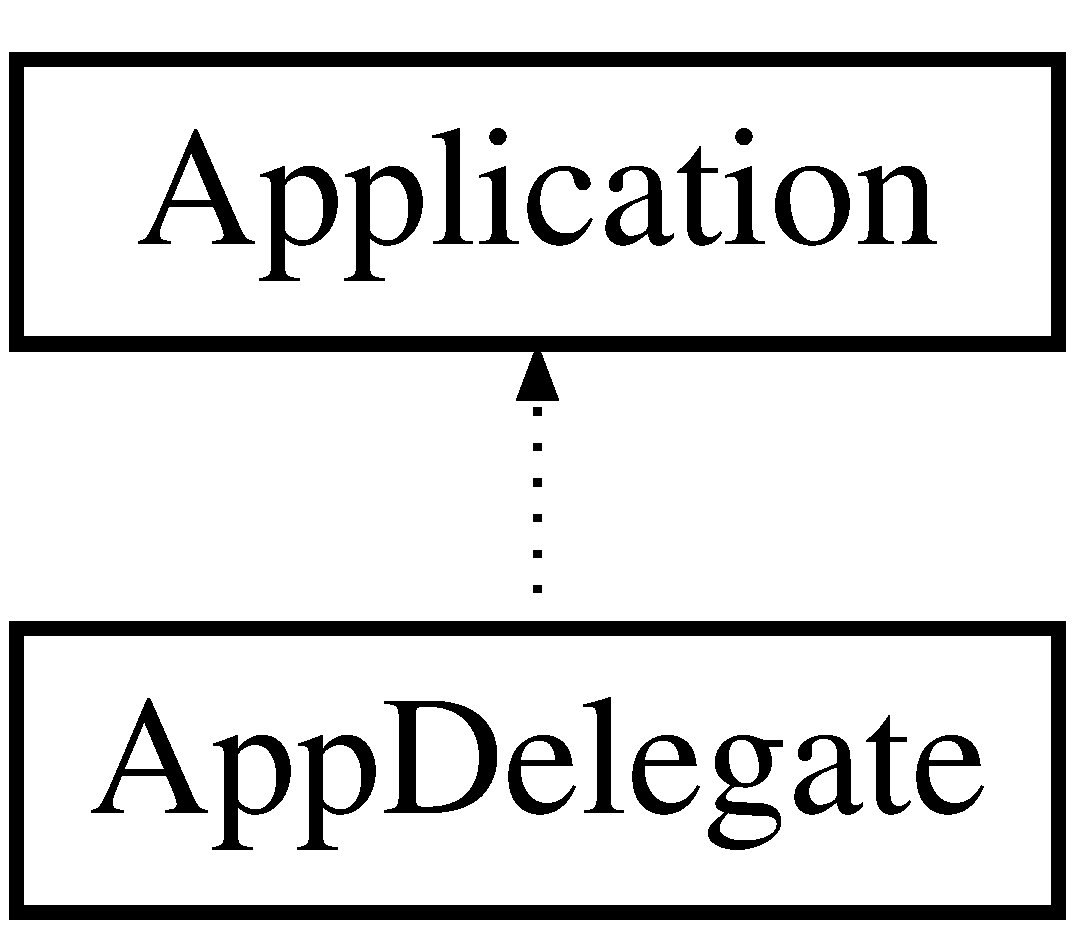
\includegraphics[height=2.000000cm]{classAppDelegate}
\end{center}
\end{figure}
\subsection*{Public Member Functions}
\begin{DoxyCompactItemize}
\item 
\hyperlink{classAppDelegate_a7d26ade6fbc9d35ecc9185792303f82d}{App\-Delegate} ()
\item 
virtual \hyperlink{classAppDelegate_a9f89424b5e296e3668deaa0265fc5ac1}{$\sim$\-App\-Delegate} ()
\item 
virtual void \hyperlink{classAppDelegate_a2de4e8ab7d04bde311684e1d4ceb2c0f}{init\-G\-L\-Context\-Attrs} ()
\item 
virtual bool \hyperlink{classAppDelegate_a68cbaed49edf7581dc59a09d5062fff3}{application\-Did\-Finish\-Launching} ()
\begin{DoxyCompactList}\small\item\em Implement Director and Scene init code here. \end{DoxyCompactList}\item 
virtual void \hyperlink{classAppDelegate_a17cb09777419781698324e0415bffd3a}{application\-Did\-Enter\-Background} ()
\begin{DoxyCompactList}\small\item\em The function be called when the application enter background. \end{DoxyCompactList}\item 
virtual void \hyperlink{classAppDelegate_ac4d653e3f74a91efef5f2def58fe3108}{application\-Will\-Enter\-Foreground} ()
\begin{DoxyCompactList}\small\item\em The function be called when the application enter foreground. \end{DoxyCompactList}\end{DoxyCompactItemize}


\subsection{Detailed Description}
The cocos2d Application. 

The reason for implement as private inheritance is to hide some interface call by Director. 

\subsection{Constructor \& Destructor Documentation}
\hypertarget{classAppDelegate_a7d26ade6fbc9d35ecc9185792303f82d}{\index{App\-Delegate@{App\-Delegate}!App\-Delegate@{App\-Delegate}}
\index{App\-Delegate@{App\-Delegate}!AppDelegate@{App\-Delegate}}
\subsubsection[{App\-Delegate}]{\setlength{\rightskip}{0pt plus 5cm}App\-Delegate\-::\-App\-Delegate (
\begin{DoxyParamCaption}
{}
\end{DoxyParamCaption}
)}}\label{classAppDelegate_a7d26ade6fbc9d35ecc9185792303f82d}
\hypertarget{classAppDelegate_a9f89424b5e296e3668deaa0265fc5ac1}{\index{App\-Delegate@{App\-Delegate}!$\sim$\-App\-Delegate@{$\sim$\-App\-Delegate}}
\index{$\sim$\-App\-Delegate@{$\sim$\-App\-Delegate}!AppDelegate@{App\-Delegate}}
\subsubsection[{$\sim$\-App\-Delegate}]{\setlength{\rightskip}{0pt plus 5cm}App\-Delegate\-::$\sim$\-App\-Delegate (
\begin{DoxyParamCaption}
{}
\end{DoxyParamCaption}
)\hspace{0.3cm}{\ttfamily [virtual]}}}\label{classAppDelegate_a9f89424b5e296e3668deaa0265fc5ac1}


\subsection{Member Function Documentation}
\hypertarget{classAppDelegate_a17cb09777419781698324e0415bffd3a}{\index{App\-Delegate@{App\-Delegate}!application\-Did\-Enter\-Background@{application\-Did\-Enter\-Background}}
\index{application\-Did\-Enter\-Background@{application\-Did\-Enter\-Background}!AppDelegate@{App\-Delegate}}
\subsubsection[{application\-Did\-Enter\-Background}]{\setlength{\rightskip}{0pt plus 5cm}void App\-Delegate\-::application\-Did\-Enter\-Background (
\begin{DoxyParamCaption}
{}
\end{DoxyParamCaption}
)\hspace{0.3cm}{\ttfamily [virtual]}}}\label{classAppDelegate_a17cb09777419781698324e0415bffd3a}


The function be called when the application enter background. 


\begin{DoxyParams}{Parameters}
{\em the} & pointer of the application \\
\hline
\end{DoxyParams}
\hypertarget{classAppDelegate_a68cbaed49edf7581dc59a09d5062fff3}{\index{App\-Delegate@{App\-Delegate}!application\-Did\-Finish\-Launching@{application\-Did\-Finish\-Launching}}
\index{application\-Did\-Finish\-Launching@{application\-Did\-Finish\-Launching}!AppDelegate@{App\-Delegate}}
\subsubsection[{application\-Did\-Finish\-Launching}]{\setlength{\rightskip}{0pt plus 5cm}bool App\-Delegate\-::application\-Did\-Finish\-Launching (
\begin{DoxyParamCaption}
{}
\end{DoxyParamCaption}
)\hspace{0.3cm}{\ttfamily [virtual]}}}\label{classAppDelegate_a68cbaed49edf7581dc59a09d5062fff3}


Implement Director and Scene init code here. 

\begin{DoxyReturn}{Returns}
true Initialize success, app continue. 

false Initialize failed, app terminate. 
\end{DoxyReturn}
\hypertarget{classAppDelegate_ac4d653e3f74a91efef5f2def58fe3108}{\index{App\-Delegate@{App\-Delegate}!application\-Will\-Enter\-Foreground@{application\-Will\-Enter\-Foreground}}
\index{application\-Will\-Enter\-Foreground@{application\-Will\-Enter\-Foreground}!AppDelegate@{App\-Delegate}}
\subsubsection[{application\-Will\-Enter\-Foreground}]{\setlength{\rightskip}{0pt plus 5cm}void App\-Delegate\-::application\-Will\-Enter\-Foreground (
\begin{DoxyParamCaption}
{}
\end{DoxyParamCaption}
)\hspace{0.3cm}{\ttfamily [virtual]}}}\label{classAppDelegate_ac4d653e3f74a91efef5f2def58fe3108}


The function be called when the application enter foreground. 


\begin{DoxyParams}{Parameters}
{\em the} & pointer of the application \\
\hline
\end{DoxyParams}
\hypertarget{classAppDelegate_a2de4e8ab7d04bde311684e1d4ceb2c0f}{\index{App\-Delegate@{App\-Delegate}!init\-G\-L\-Context\-Attrs@{init\-G\-L\-Context\-Attrs}}
\index{init\-G\-L\-Context\-Attrs@{init\-G\-L\-Context\-Attrs}!AppDelegate@{App\-Delegate}}
\subsubsection[{init\-G\-L\-Context\-Attrs}]{\setlength{\rightskip}{0pt plus 5cm}void App\-Delegate\-::init\-G\-L\-Context\-Attrs (
\begin{DoxyParamCaption}
{}
\end{DoxyParamCaption}
)\hspace{0.3cm}{\ttfamily [virtual]}}}\label{classAppDelegate_a2de4e8ab7d04bde311684e1d4ceb2c0f}


The documentation for this class was generated from the following files\-:\begin{DoxyCompactItemize}
\item 
\hyperlink{AppDelegate_8h}{App\-Delegate.\-h}\item 
\hyperlink{AppDelegate_8cpp}{App\-Delegate.\-cpp}\end{DoxyCompactItemize}

\hypertarget{classBase}{\section{Base Class Reference}
\label{classBase}\index{Base@{Base}}
}


All objects which have an I\-D and U\-I\-D inherit from \hyperlink{classBase}{Base}.  




{\ttfamily \#include $<$Base.\-h$>$}

Inheritance diagram for Base\-:\begin{figure}[H]
\begin{center}
\leavevmode
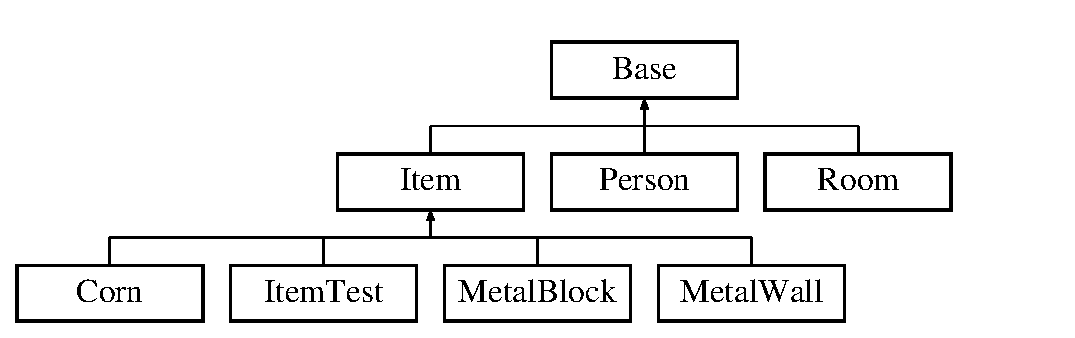
\includegraphics[height=3.000000cm]{classBase}
\end{center}
\end{figure}
\subsection*{Public Member Functions}
\begin{DoxyCompactItemize}
\item 
\hyperlink{classBase_a5ffe0568374d8b9b4c4ec32953fd6453}{Base} ()
\end{DoxyCompactItemize}
\subsection*{Public Attributes}
\begin{DoxyCompactItemize}
\item 
int \hyperlink{classBase_ac25c86b1d7bb8304fc0a81b8bddf7faf}{U\-I\-D}
\begin{DoxyCompactList}\small\item\em Unique I\-D. Often used to find a spesific object. \end{DoxyCompactList}\item 
int \hyperlink{classBase_a1dddc037afe2eae3e1364597e6a3cf46}{I\-D}
\begin{DoxyCompactList}\small\item\em I\-D spesifies the type of the object, useful for casting. \end{DoxyCompactList}\end{DoxyCompactItemize}


\subsection{Detailed Description}
All objects which have an I\-D and U\-I\-D inherit from \hyperlink{classBase}{Base}. 

\subsection{Constructor \& Destructor Documentation}
\hypertarget{classBase_a5ffe0568374d8b9b4c4ec32953fd6453}{\index{Base@{Base}!Base@{Base}}
\index{Base@{Base}!Base@{Base}}
\subsubsection[{Base}]{\setlength{\rightskip}{0pt plus 5cm}Base\-::\-Base (
\begin{DoxyParamCaption}
{}
\end{DoxyParamCaption}
)}}\label{classBase_a5ffe0568374d8b9b4c4ec32953fd6453}


\subsection{Member Data Documentation}
\hypertarget{classBase_a1dddc037afe2eae3e1364597e6a3cf46}{\index{Base@{Base}!I\-D@{I\-D}}
\index{I\-D@{I\-D}!Base@{Base}}
\subsubsection[{I\-D}]{\setlength{\rightskip}{0pt plus 5cm}int Base\-::\-I\-D}}\label{classBase_a1dddc037afe2eae3e1364597e6a3cf46}


I\-D spesifies the type of the object, useful for casting. 

\hypertarget{classBase_ac25c86b1d7bb8304fc0a81b8bddf7faf}{\index{Base@{Base}!U\-I\-D@{U\-I\-D}}
\index{U\-I\-D@{U\-I\-D}!Base@{Base}}
\subsubsection[{U\-I\-D}]{\setlength{\rightskip}{0pt plus 5cm}int Base\-::\-U\-I\-D}}\label{classBase_ac25c86b1d7bb8304fc0a81b8bddf7faf}


Unique I\-D. Often used to find a spesific object. 



The documentation for this class was generated from the following files\-:\begin{DoxyCompactItemize}
\item 
core/\hyperlink{Base_8h}{Base.\-h}\item 
core/\hyperlink{Base_8cpp}{Base.\-cpp}\end{DoxyCompactItemize}

\hypertarget{classCorn}{\section{Corn Class Reference}
\label{classCorn}\index{Corn@{Corn}}
}


{\ttfamily \#include $<$Corn.\-h$>$}

Inheritance diagram for Corn\-:\begin{figure}[H]
\begin{center}
\leavevmode
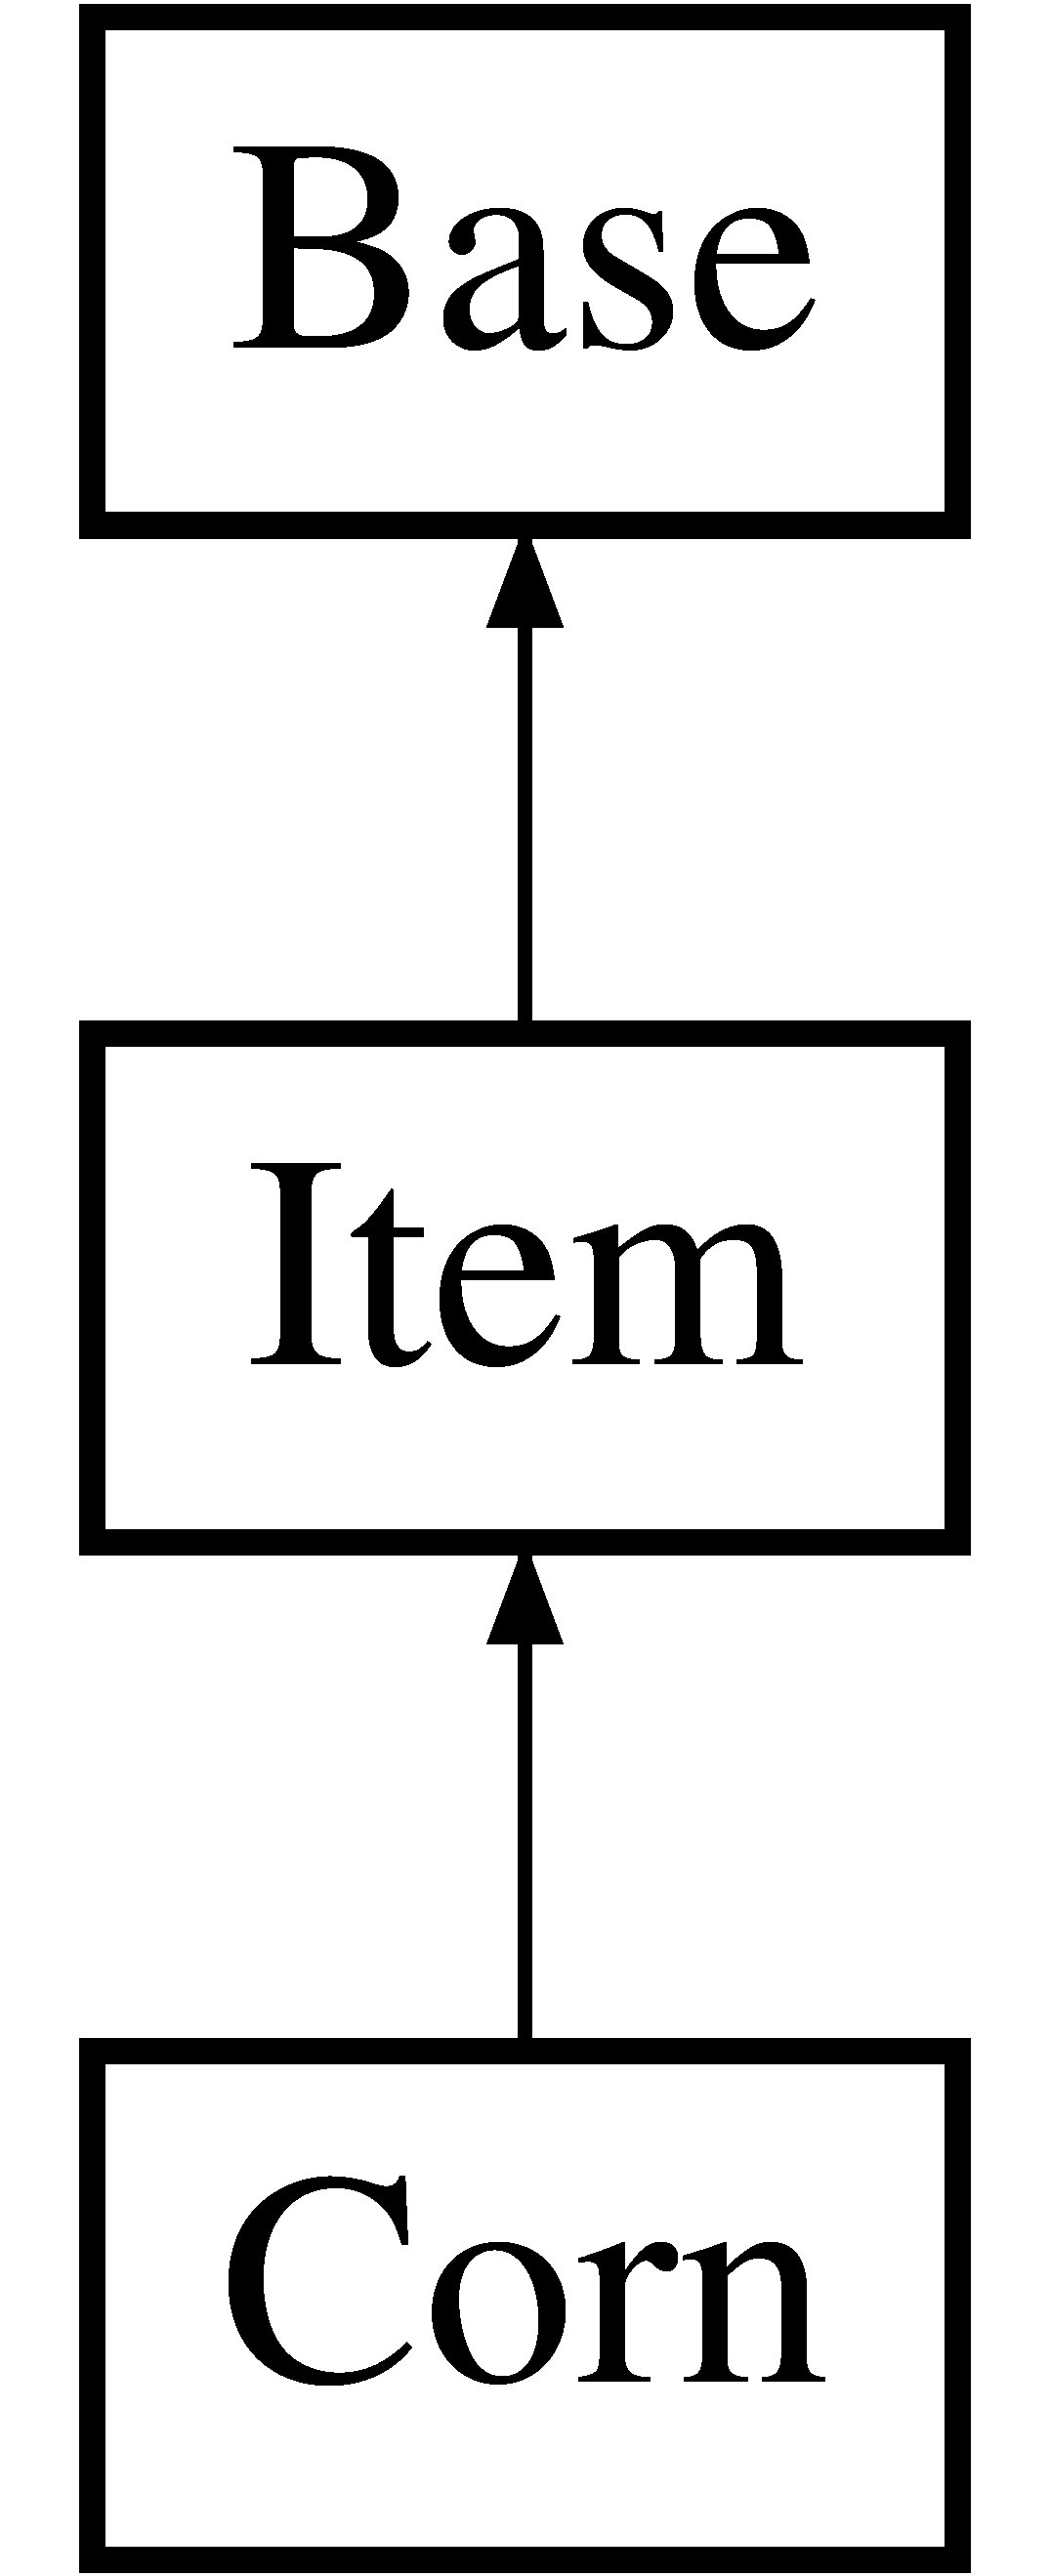
\includegraphics[height=3.000000cm]{classCorn}
\end{center}
\end{figure}
\subsection*{Public Member Functions}
\begin{DoxyCompactItemize}
\item 
\hyperlink{classCorn_a6857f6bbbd53d8eb29a5f7b0a4b438b9}{Corn} ()
\item 
void \hyperlink{classCorn_aa7e9de2a19263681f7a3248ba821321f}{grow} ()
\item 
void \hyperlink{classCorn_a7fdd2972e5d706de8cf64bd6c2eae2a3}{reset} ()
\item 
void \hyperlink{classCorn_ab9eee4022f2efe2142e987c3bed88a43}{update} (\hyperlink{classShipMaster}{Ship\-Master} \&ship)
\item 
int \hyperlink{classCorn_ac0b6aa014ed83b6c488cf8e77b0f7822}{get\-Texture\-I\-D} ()
\item 
void \hyperlink{classCorn_a6113c52b8a1c3d3e49a5a9908b4375a1}{update} ()
\item 
bool \hyperlink{classCorn_aa3aef7eecbd7cb36a85cdb7d5acd9f28}{interact} (\hyperlink{classPerson}{Person} \&person)
\item 
bool \hyperlink{classCorn_a4554f0e4db0d59d303749c76310d4476}{place} (\hyperlink{classPerson}{Person} \&person)
\item 
bool \hyperlink{classCorn_a120e5ee8556cff62e32ad81456a8809f}{can\-Place} (\hyperlink{classPerson}{Person} \&person)
\item 
bool \hyperlink{classCorn_a717e3de78f91990dce16c33743d9c38f}{is\-Finished} ()
\item 
int \hyperlink{classCorn_a77a736dbaaefb04a913ce461a46b4d0c}{get\-Stage} ()
\end{DoxyCompactItemize}
\subsection*{Public Attributes}
\begin{DoxyCompactItemize}
\item 
bool \hyperlink{classCorn_a1b3eeae171a4920a7816acc8e3d15877}{changed}
\item 
int \hyperlink{classCorn_af36e334c7841e04e5e2057e4622efc35}{stage}
\item 
int \hyperlink{classCorn_ae07bb9fe1250f25d9263e15906d05b11}{time}
\end{DoxyCompactItemize}
\subsection*{Static Public Attributes}
\begin{DoxyCompactItemize}
\item 
static const int \hyperlink{classCorn_a06dcd52a729fca8910331e6a2fd59224}{S\-T\-A\-G\-E\-\_\-0} = 5
\item 
static const int \hyperlink{classCorn_ac82c4d495b1f3337e56adcde2d44bdba}{S\-T\-A\-G\-E\-\_\-1} = 10
\item 
static const int \hyperlink{classCorn_a098322daae5849ac79fb71a39475376d}{S\-T\-A\-G\-E\-\_\-2} = 15
\item 
static const int \hyperlink{classCorn_ae27fd5a47e3b83c96f459eb26a9c89d9}{S\-T\-A\-G\-E\-\_\-\-F\-I\-N\-A\-L} = \hyperlink{classCorn_a098322daae5849ac79fb71a39475376d}{S\-T\-A\-G\-E\-\_\-2}
\end{DoxyCompactItemize}
\subsection*{Additional Inherited Members}


\subsection{Constructor \& Destructor Documentation}
\hypertarget{classCorn_a6857f6bbbd53d8eb29a5f7b0a4b438b9}{\index{Corn@{Corn}!Corn@{Corn}}
\index{Corn@{Corn}!Corn@{Corn}}
\subsubsection[{Corn}]{\setlength{\rightskip}{0pt plus 5cm}Corn\-::\-Corn (
\begin{DoxyParamCaption}
{}
\end{DoxyParamCaption}
)}}\label{classCorn_a6857f6bbbd53d8eb29a5f7b0a4b438b9}


\subsection{Member Function Documentation}
\hypertarget{classCorn_a120e5ee8556cff62e32ad81456a8809f}{\index{Corn@{Corn}!can\-Place@{can\-Place}}
\index{can\-Place@{can\-Place}!Corn@{Corn}}
\subsubsection[{can\-Place}]{\setlength{\rightskip}{0pt plus 5cm}bool Corn\-::can\-Place (
\begin{DoxyParamCaption}
\item[{{\bf Person} \&}]{person}
\end{DoxyParamCaption}
)\hspace{0.3cm}{\ttfamily [virtual]}}}\label{classCorn_a120e5ee8556cff62e32ad81456a8809f}


Implements \hyperlink{classItem_afa9967b10984b1886ed6097eab7239e3}{Item}.

\hypertarget{classCorn_a77a736dbaaefb04a913ce461a46b4d0c}{\index{Corn@{Corn}!get\-Stage@{get\-Stage}}
\index{get\-Stage@{get\-Stage}!Corn@{Corn}}
\subsubsection[{get\-Stage}]{\setlength{\rightskip}{0pt plus 5cm}int Corn\-::get\-Stage (
\begin{DoxyParamCaption}
{}
\end{DoxyParamCaption}
)}}\label{classCorn_a77a736dbaaefb04a913ce461a46b4d0c}
\hypertarget{classCorn_ac0b6aa014ed83b6c488cf8e77b0f7822}{\index{Corn@{Corn}!get\-Texture\-I\-D@{get\-Texture\-I\-D}}
\index{get\-Texture\-I\-D@{get\-Texture\-I\-D}!Corn@{Corn}}
\subsubsection[{get\-Texture\-I\-D}]{\setlength{\rightskip}{0pt plus 5cm}int Corn\-::get\-Texture\-I\-D (
\begin{DoxyParamCaption}
{}
\end{DoxyParamCaption}
)\hspace{0.3cm}{\ttfamily [virtual]}}}\label{classCorn_ac0b6aa014ed83b6c488cf8e77b0f7822}


Implements \hyperlink{classItem_a38889163e99a1f5ec9b811b8e64fbc36}{Item}.

\hypertarget{classCorn_aa7e9de2a19263681f7a3248ba821321f}{\index{Corn@{Corn}!grow@{grow}}
\index{grow@{grow}!Corn@{Corn}}
\subsubsection[{grow}]{\setlength{\rightskip}{0pt plus 5cm}void Corn\-::grow (
\begin{DoxyParamCaption}
{}
\end{DoxyParamCaption}
)}}\label{classCorn_aa7e9de2a19263681f7a3248ba821321f}
\hypertarget{classCorn_aa3aef7eecbd7cb36a85cdb7d5acd9f28}{\index{Corn@{Corn}!interact@{interact}}
\index{interact@{interact}!Corn@{Corn}}
\subsubsection[{interact}]{\setlength{\rightskip}{0pt plus 5cm}bool Corn\-::interact (
\begin{DoxyParamCaption}
\item[{{\bf Person} \&}]{person}
\end{DoxyParamCaption}
)\hspace{0.3cm}{\ttfamily [virtual]}}}\label{classCorn_aa3aef7eecbd7cb36a85cdb7d5acd9f28}


Implements \hyperlink{classItem_a65a4d68109b4aa82c62d262ab4786145}{Item}.

\hypertarget{classCorn_a717e3de78f91990dce16c33743d9c38f}{\index{Corn@{Corn}!is\-Finished@{is\-Finished}}
\index{is\-Finished@{is\-Finished}!Corn@{Corn}}
\subsubsection[{is\-Finished}]{\setlength{\rightskip}{0pt plus 5cm}bool Corn\-::is\-Finished (
\begin{DoxyParamCaption}
{}
\end{DoxyParamCaption}
)}}\label{classCorn_a717e3de78f91990dce16c33743d9c38f}
\hypertarget{classCorn_a4554f0e4db0d59d303749c76310d4476}{\index{Corn@{Corn}!place@{place}}
\index{place@{place}!Corn@{Corn}}
\subsubsection[{place}]{\setlength{\rightskip}{0pt plus 5cm}bool Corn\-::place (
\begin{DoxyParamCaption}
\item[{{\bf Person} \&}]{person}
\end{DoxyParamCaption}
)\hspace{0.3cm}{\ttfamily [virtual]}}}\label{classCorn_a4554f0e4db0d59d303749c76310d4476}


Implements \hyperlink{classItem_a2fc04b2fdd729977c419e0a1c5c8fa87}{Item}.

\hypertarget{classCorn_a7fdd2972e5d706de8cf64bd6c2eae2a3}{\index{Corn@{Corn}!reset@{reset}}
\index{reset@{reset}!Corn@{Corn}}
\subsubsection[{reset}]{\setlength{\rightskip}{0pt plus 5cm}void Corn\-::reset (
\begin{DoxyParamCaption}
{}
\end{DoxyParamCaption}
)}}\label{classCorn_a7fdd2972e5d706de8cf64bd6c2eae2a3}
\hypertarget{classCorn_ab9eee4022f2efe2142e987c3bed88a43}{\index{Corn@{Corn}!update@{update}}
\index{update@{update}!Corn@{Corn}}
\subsubsection[{update}]{\setlength{\rightskip}{0pt plus 5cm}void Corn\-::update (
\begin{DoxyParamCaption}
\item[{{\bf Ship\-Master} \&}]{ship}
\end{DoxyParamCaption}
)\hspace{0.3cm}{\ttfamily [virtual]}}}\label{classCorn_ab9eee4022f2efe2142e987c3bed88a43}


Implements \hyperlink{classItem_af7cb35b77955c00a38fc0f952da762f4}{Item}.

\hypertarget{classCorn_a6113c52b8a1c3d3e49a5a9908b4375a1}{\index{Corn@{Corn}!update@{update}}
\index{update@{update}!Corn@{Corn}}
\subsubsection[{update}]{\setlength{\rightskip}{0pt plus 5cm}void Corn\-::update (
\begin{DoxyParamCaption}
{}
\end{DoxyParamCaption}
)}}\label{classCorn_a6113c52b8a1c3d3e49a5a9908b4375a1}


\subsection{Member Data Documentation}
\hypertarget{classCorn_a1b3eeae171a4920a7816acc8e3d15877}{\index{Corn@{Corn}!changed@{changed}}
\index{changed@{changed}!Corn@{Corn}}
\subsubsection[{changed}]{\setlength{\rightskip}{0pt plus 5cm}bool Corn\-::changed}}\label{classCorn_a1b3eeae171a4920a7816acc8e3d15877}
\hypertarget{classCorn_af36e334c7841e04e5e2057e4622efc35}{\index{Corn@{Corn}!stage@{stage}}
\index{stage@{stage}!Corn@{Corn}}
\subsubsection[{stage}]{\setlength{\rightskip}{0pt plus 5cm}int Corn\-::stage}}\label{classCorn_af36e334c7841e04e5e2057e4622efc35}
\hypertarget{classCorn_a06dcd52a729fca8910331e6a2fd59224}{\index{Corn@{Corn}!S\-T\-A\-G\-E\-\_\-0@{S\-T\-A\-G\-E\-\_\-0}}
\index{S\-T\-A\-G\-E\-\_\-0@{S\-T\-A\-G\-E\-\_\-0}!Corn@{Corn}}
\subsubsection[{S\-T\-A\-G\-E\-\_\-0}]{\setlength{\rightskip}{0pt plus 5cm}const int Corn\-::\-S\-T\-A\-G\-E\-\_\-0 = 5\hspace{0.3cm}{\ttfamily [static]}}}\label{classCorn_a06dcd52a729fca8910331e6a2fd59224}
\hypertarget{classCorn_ac82c4d495b1f3337e56adcde2d44bdba}{\index{Corn@{Corn}!S\-T\-A\-G\-E\-\_\-1@{S\-T\-A\-G\-E\-\_\-1}}
\index{S\-T\-A\-G\-E\-\_\-1@{S\-T\-A\-G\-E\-\_\-1}!Corn@{Corn}}
\subsubsection[{S\-T\-A\-G\-E\-\_\-1}]{\setlength{\rightskip}{0pt plus 5cm}const int Corn\-::\-S\-T\-A\-G\-E\-\_\-1 = 10\hspace{0.3cm}{\ttfamily [static]}}}\label{classCorn_ac82c4d495b1f3337e56adcde2d44bdba}
\hypertarget{classCorn_a098322daae5849ac79fb71a39475376d}{\index{Corn@{Corn}!S\-T\-A\-G\-E\-\_\-2@{S\-T\-A\-G\-E\-\_\-2}}
\index{S\-T\-A\-G\-E\-\_\-2@{S\-T\-A\-G\-E\-\_\-2}!Corn@{Corn}}
\subsubsection[{S\-T\-A\-G\-E\-\_\-2}]{\setlength{\rightskip}{0pt plus 5cm}const int Corn\-::\-S\-T\-A\-G\-E\-\_\-2 = 15\hspace{0.3cm}{\ttfamily [static]}}}\label{classCorn_a098322daae5849ac79fb71a39475376d}
\hypertarget{classCorn_ae27fd5a47e3b83c96f459eb26a9c89d9}{\index{Corn@{Corn}!S\-T\-A\-G\-E\-\_\-\-F\-I\-N\-A\-L@{S\-T\-A\-G\-E\-\_\-\-F\-I\-N\-A\-L}}
\index{S\-T\-A\-G\-E\-\_\-\-F\-I\-N\-A\-L@{S\-T\-A\-G\-E\-\_\-\-F\-I\-N\-A\-L}!Corn@{Corn}}
\subsubsection[{S\-T\-A\-G\-E\-\_\-\-F\-I\-N\-A\-L}]{\setlength{\rightskip}{0pt plus 5cm}const int Corn\-::\-S\-T\-A\-G\-E\-\_\-\-F\-I\-N\-A\-L = {\bf S\-T\-A\-G\-E\-\_\-2}\hspace{0.3cm}{\ttfamily [static]}}}\label{classCorn_ae27fd5a47e3b83c96f459eb26a9c89d9}
\hypertarget{classCorn_ae07bb9fe1250f25d9263e15906d05b11}{\index{Corn@{Corn}!time@{time}}
\index{time@{time}!Corn@{Corn}}
\subsubsection[{time}]{\setlength{\rightskip}{0pt plus 5cm}int Corn\-::time}}\label{classCorn_ae07bb9fe1250f25d9263e15906d05b11}


The documentation for this class was generated from the following files\-:\begin{DoxyCompactItemize}
\item 
core/items/\hyperlink{Corn_8h}{Corn.\-h}\item 
core/items/\hyperlink{Corn_8cpp}{Corn.\-cpp}\end{DoxyCompactItemize}

\hypertarget{classHelloWorld}{\section{Hello\-World Class Reference}
\label{classHelloWorld}\index{Hello\-World@{Hello\-World}}
}


{\ttfamily \#include $<$Hello\-World\-Scene.\-h$>$}

Inheritance diagram for Hello\-World\-:\begin{figure}[H]
\begin{center}
\leavevmode
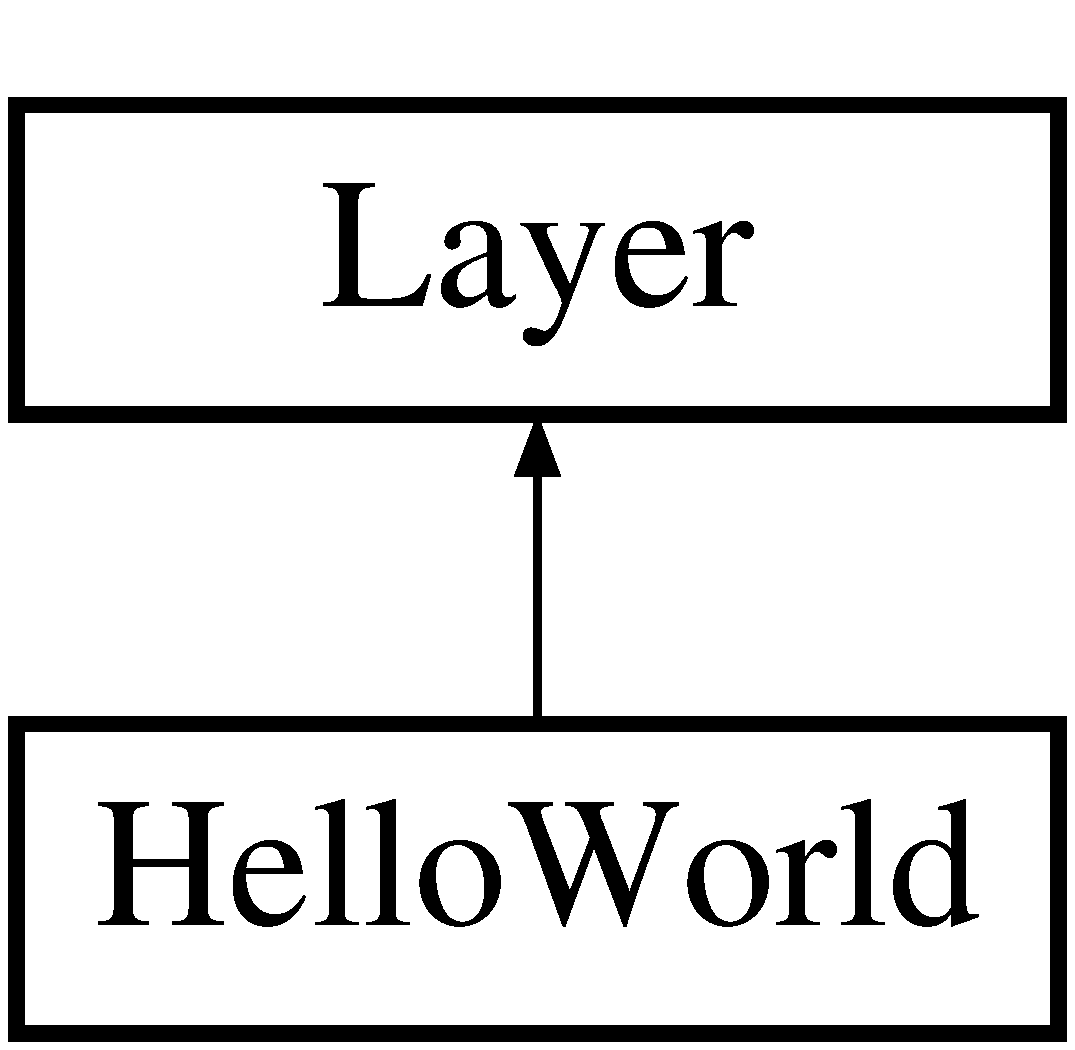
\includegraphics[height=2.000000cm]{classHelloWorld}
\end{center}
\end{figure}
\subsection*{Public Member Functions}
\begin{DoxyCompactItemize}
\item 
virtual bool \hyperlink{classHelloWorld_a65e2b1525051f3690e5a39ca56608a97}{init} ()
\item 
void \hyperlink{classHelloWorld_ac4ab2f5e922e659d4f137591c0f6a9b0}{menu\-Close\-Callback} (cocos2d\-::\-Ref $\ast$p\-Sender)
\item 
void \hyperlink{classHelloWorld_acf5d9777877c1b475a6c4bc1c16fac8a}{update} (float) override
\item 
\hyperlink{classHelloWorld_a857ebfbc49f3a7f81772bee4991d186b}{C\-R\-E\-A\-T\-E\-\_\-\-F\-U\-N\-C} (\hyperlink{classHelloWorld}{Hello\-World})
\end{DoxyCompactItemize}
\subsection*{Static Public Member Functions}
\begin{DoxyCompactItemize}
\item 
static cocos2d\-::\-Scene $\ast$ \hyperlink{classHelloWorld_a1b700f5f9de04271533d3fa099d7b014}{create\-Scene} ()
\end{DoxyCompactItemize}


\subsection{Member Function Documentation}
\hypertarget{classHelloWorld_a857ebfbc49f3a7f81772bee4991d186b}{\index{Hello\-World@{Hello\-World}!C\-R\-E\-A\-T\-E\-\_\-\-F\-U\-N\-C@{C\-R\-E\-A\-T\-E\-\_\-\-F\-U\-N\-C}}
\index{C\-R\-E\-A\-T\-E\-\_\-\-F\-U\-N\-C@{C\-R\-E\-A\-T\-E\-\_\-\-F\-U\-N\-C}!HelloWorld@{Hello\-World}}
\subsubsection[{C\-R\-E\-A\-T\-E\-\_\-\-F\-U\-N\-C}]{\setlength{\rightskip}{0pt plus 5cm}Hello\-World\-::\-C\-R\-E\-A\-T\-E\-\_\-\-F\-U\-N\-C (
\begin{DoxyParamCaption}
\item[{{\bf Hello\-World}}]{}
\end{DoxyParamCaption}
)}}\label{classHelloWorld_a857ebfbc49f3a7f81772bee4991d186b}
\hypertarget{classHelloWorld_a1b700f5f9de04271533d3fa099d7b014}{\index{Hello\-World@{Hello\-World}!create\-Scene@{create\-Scene}}
\index{create\-Scene@{create\-Scene}!HelloWorld@{Hello\-World}}
\subsubsection[{create\-Scene}]{\setlength{\rightskip}{0pt plus 5cm}Scene $\ast$ Hello\-World\-::create\-Scene (
\begin{DoxyParamCaption}
{}
\end{DoxyParamCaption}
)\hspace{0.3cm}{\ttfamily [static]}}}\label{classHelloWorld_a1b700f5f9de04271533d3fa099d7b014}
\hypertarget{classHelloWorld_a65e2b1525051f3690e5a39ca56608a97}{\index{Hello\-World@{Hello\-World}!init@{init}}
\index{init@{init}!HelloWorld@{Hello\-World}}
\subsubsection[{init}]{\setlength{\rightskip}{0pt plus 5cm}bool Hello\-World\-::init (
\begin{DoxyParamCaption}
{}
\end{DoxyParamCaption}
)\hspace{0.3cm}{\ttfamily [virtual]}}}\label{classHelloWorld_a65e2b1525051f3690e5a39ca56608a97}
\hypertarget{classHelloWorld_ac4ab2f5e922e659d4f137591c0f6a9b0}{\index{Hello\-World@{Hello\-World}!menu\-Close\-Callback@{menu\-Close\-Callback}}
\index{menu\-Close\-Callback@{menu\-Close\-Callback}!HelloWorld@{Hello\-World}}
\subsubsection[{menu\-Close\-Callback}]{\setlength{\rightskip}{0pt plus 5cm}void Hello\-World\-::menu\-Close\-Callback (
\begin{DoxyParamCaption}
\item[{cocos2d\-::\-Ref $\ast$}]{p\-Sender}
\end{DoxyParamCaption}
)}}\label{classHelloWorld_ac4ab2f5e922e659d4f137591c0f6a9b0}
\hypertarget{classHelloWorld_acf5d9777877c1b475a6c4bc1c16fac8a}{\index{Hello\-World@{Hello\-World}!update@{update}}
\index{update@{update}!HelloWorld@{Hello\-World}}
\subsubsection[{update}]{\setlength{\rightskip}{0pt plus 5cm}void Hello\-World\-::update (
\begin{DoxyParamCaption}
\item[{float}]{dt}
\end{DoxyParamCaption}
)\hspace{0.3cm}{\ttfamily [override]}}}\label{classHelloWorld_acf5d9777877c1b475a6c4bc1c16fac8a}


The documentation for this class was generated from the following files\-:\begin{DoxyCompactItemize}
\item 
\hyperlink{HelloWorldScene_8h}{Hello\-World\-Scene.\-h}\item 
\hyperlink{HelloWorldScene_8cpp}{Hello\-World\-Scene.\-cpp}\end{DoxyCompactItemize}

\hypertarget{classItem}{\section{Item Class Reference}
\label{classItem}\index{Item@{Item}}
}


{\ttfamily \#include $<$Item.\-h$>$}

Inheritance diagram for Item\-:\begin{figure}[H]
\begin{center}
\leavevmode
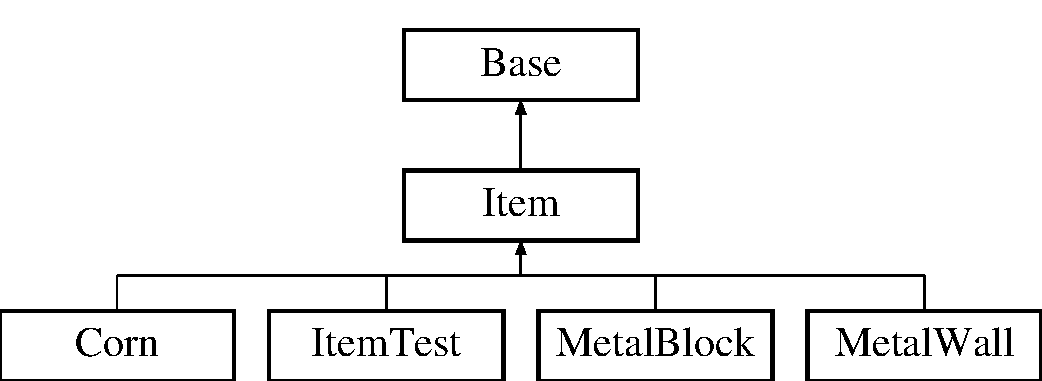
\includegraphics[height=3.000000cm]{classItem}
\end{center}
\end{figure}
\subsection*{Public Member Functions}
\begin{DoxyCompactItemize}
\item 
\hyperlink{classItem_aeccb01d448bffa2c4b89a49d4d39ea6f}{Item} (int \hyperlink{classBase_a1dddc037afe2eae3e1364597e6a3cf46}{I\-D}, int \hyperlink{classItem_adcfbfc3a87d2112c62b812dac2c72993}{slot}, int \hyperlink{classItem_a5166900b24ba9e746a7ad34c00353cdd}{blocking})
\item 
virtual \hyperlink{classItem_a33cc9c0bc556b5a33a9d0d58d37c602b}{$\sim$\-Item} ()
\item 
virtual void \hyperlink{classItem_af7cb35b77955c00a38fc0f952da762f4}{update} (\hyperlink{classShipMaster}{Ship\-Master} \&ship)=0
\item 
virtual bool \hyperlink{classItem_a65a4d68109b4aa82c62d262ab4786145}{interact} (\hyperlink{classPerson}{Person} \&person)=0
\item 
virtual bool \hyperlink{classItem_a2fc04b2fdd729977c419e0a1c5c8fa87}{place} (\hyperlink{classPerson}{Person} \&person)=0
\item 
virtual bool \hyperlink{classItem_afa9967b10984b1886ed6097eab7239e3}{can\-Place} (\hyperlink{classPerson}{Person} \&person)=0
\item 
virtual int \hyperlink{classItem_a38889163e99a1f5ec9b811b8e64fbc36}{get\-Texture\-I\-D} ()=0
\item 
virtual void \hyperlink{classItem_aa4aea30738280ffbc897ed3a9b64362a}{set\-Direction} (int \hyperlink{classItem_a1812b51dc93d2142c0641c536fbef617}{direction})
\item 
void \hyperlink{classItem_ab347bc647966f28266a36e3af34c35cc}{set\-Placed} (bool val)
\item 
bool \hyperlink{classItem_aca2ca239027e41044ce015c14c4feff6}{is\-Placed} ()
\item 
int \hyperlink{classItem_a9f232e560cdaec93805b428349477c68}{get\-Direction} ()
\end{DoxyCompactItemize}
\subsection*{Public Attributes}
\begin{DoxyCompactItemize}
\item 
\hyperlink{structLocation}{Location} \hyperlink{classItem_ade907eeeea58df68fcacde1e5568779b}{loc}
\item 
int \hyperlink{classItem_adcfbfc3a87d2112c62b812dac2c72993}{slot}
\item 
int \hyperlink{classItem_a5166900b24ba9e746a7ad34c00353cdd}{blocking}
\end{DoxyCompactItemize}
\subsection*{Protected Attributes}
\begin{DoxyCompactItemize}
\item 
int \hyperlink{classItem_a1812b51dc93d2142c0641c536fbef617}{direction}
\end{DoxyCompactItemize}


\subsection{Constructor \& Destructor Documentation}
\hypertarget{classItem_aeccb01d448bffa2c4b89a49d4d39ea6f}{\index{Item@{Item}!Item@{Item}}
\index{Item@{Item}!Item@{Item}}
\subsubsection[{Item}]{\setlength{\rightskip}{0pt plus 5cm}Item\-::\-Item (
\begin{DoxyParamCaption}
\item[{int}]{I\-D, }
\item[{int}]{slot, }
\item[{int}]{blocking}
\end{DoxyParamCaption}
)\hspace{0.3cm}{\ttfamily [inline]}}}\label{classItem_aeccb01d448bffa2c4b89a49d4d39ea6f}
\hypertarget{classItem_a33cc9c0bc556b5a33a9d0d58d37c602b}{\index{Item@{Item}!$\sim$\-Item@{$\sim$\-Item}}
\index{$\sim$\-Item@{$\sim$\-Item}!Item@{Item}}
\subsubsection[{$\sim$\-Item}]{\setlength{\rightskip}{0pt plus 5cm}virtual Item\-::$\sim$\-Item (
\begin{DoxyParamCaption}
{}
\end{DoxyParamCaption}
)\hspace{0.3cm}{\ttfamily [inline]}, {\ttfamily [virtual]}}}\label{classItem_a33cc9c0bc556b5a33a9d0d58d37c602b}


\subsection{Member Function Documentation}
\hypertarget{classItem_afa9967b10984b1886ed6097eab7239e3}{\index{Item@{Item}!can\-Place@{can\-Place}}
\index{can\-Place@{can\-Place}!Item@{Item}}
\subsubsection[{can\-Place}]{\setlength{\rightskip}{0pt plus 5cm}virtual bool Item\-::can\-Place (
\begin{DoxyParamCaption}
\item[{{\bf Person} \&}]{person}
\end{DoxyParamCaption}
)\hspace{0.3cm}{\ttfamily [pure virtual]}}}\label{classItem_afa9967b10984b1886ed6097eab7239e3}


Implemented in \hyperlink{structItemTest_a22ad8ab142e30bc5b1d45425ed1d26b5}{Item\-Test}, \hyperlink{classCorn_a120e5ee8556cff62e32ad81456a8809f}{Corn}, \hyperlink{classMetalBlock_a3ebb02bfb392a81c292d8f1fa0e7054e}{Metal\-Block}, and \hyperlink{classMetalWall_acd888cb6afaa418a3a92f14eda27a9a5}{Metal\-Wall}.

\hypertarget{classItem_a9f232e560cdaec93805b428349477c68}{\index{Item@{Item}!get\-Direction@{get\-Direction}}
\index{get\-Direction@{get\-Direction}!Item@{Item}}
\subsubsection[{get\-Direction}]{\setlength{\rightskip}{0pt plus 5cm}int Item\-::get\-Direction (
\begin{DoxyParamCaption}
{}
\end{DoxyParamCaption}
)\hspace{0.3cm}{\ttfamily [inline]}}}\label{classItem_a9f232e560cdaec93805b428349477c68}
\hypertarget{classItem_a38889163e99a1f5ec9b811b8e64fbc36}{\index{Item@{Item}!get\-Texture\-I\-D@{get\-Texture\-I\-D}}
\index{get\-Texture\-I\-D@{get\-Texture\-I\-D}!Item@{Item}}
\subsubsection[{get\-Texture\-I\-D}]{\setlength{\rightskip}{0pt plus 5cm}virtual int Item\-::get\-Texture\-I\-D (
\begin{DoxyParamCaption}
{}
\end{DoxyParamCaption}
)\hspace{0.3cm}{\ttfamily [pure virtual]}}}\label{classItem_a38889163e99a1f5ec9b811b8e64fbc36}


Implemented in \hyperlink{structItemTest_a040963d27bd3bc753664ece6845f9650}{Item\-Test}, \hyperlink{classMetalBlock_aed60769587273b97c098defb6bb19a0f}{Metal\-Block}, \hyperlink{classMetalWall_a2c647de3c51c744da75cae0096e0042d}{Metal\-Wall}, and \hyperlink{classCorn_ac0b6aa014ed83b6c488cf8e77b0f7822}{Corn}.

\hypertarget{classItem_a65a4d68109b4aa82c62d262ab4786145}{\index{Item@{Item}!interact@{interact}}
\index{interact@{interact}!Item@{Item}}
\subsubsection[{interact}]{\setlength{\rightskip}{0pt plus 5cm}virtual bool Item\-::interact (
\begin{DoxyParamCaption}
\item[{{\bf Person} \&}]{person}
\end{DoxyParamCaption}
)\hspace{0.3cm}{\ttfamily [pure virtual]}}}\label{classItem_a65a4d68109b4aa82c62d262ab4786145}


Implemented in \hyperlink{structItemTest_a75e6ddccebab853a259a0957c15407e1}{Item\-Test}, \hyperlink{classCorn_aa3aef7eecbd7cb36a85cdb7d5acd9f28}{Corn}, \hyperlink{classMetalBlock_ae5da009046d9443f292fbf7d955d3dc9}{Metal\-Block}, and \hyperlink{classMetalWall_a6c5791ba1b0f1c4c6b9f064ceb0d217d}{Metal\-Wall}.

\hypertarget{classItem_aca2ca239027e41044ce015c14c4feff6}{\index{Item@{Item}!is\-Placed@{is\-Placed}}
\index{is\-Placed@{is\-Placed}!Item@{Item}}
\subsubsection[{is\-Placed}]{\setlength{\rightskip}{0pt plus 5cm}bool Item\-::is\-Placed (
\begin{DoxyParamCaption}
{}
\end{DoxyParamCaption}
)\hspace{0.3cm}{\ttfamily [inline]}}}\label{classItem_aca2ca239027e41044ce015c14c4feff6}
\hypertarget{classItem_a2fc04b2fdd729977c419e0a1c5c8fa87}{\index{Item@{Item}!place@{place}}
\index{place@{place}!Item@{Item}}
\subsubsection[{place}]{\setlength{\rightskip}{0pt plus 5cm}virtual bool Item\-::place (
\begin{DoxyParamCaption}
\item[{{\bf Person} \&}]{person}
\end{DoxyParamCaption}
)\hspace{0.3cm}{\ttfamily [pure virtual]}}}\label{classItem_a2fc04b2fdd729977c419e0a1c5c8fa87}


Implemented in \hyperlink{structItemTest_ad30228b68d1b22411270e6b304a87249}{Item\-Test}, \hyperlink{classCorn_a4554f0e4db0d59d303749c76310d4476}{Corn}, \hyperlink{classMetalBlock_a58537a96320a39f4c46659994698c394}{Metal\-Block}, and \hyperlink{classMetalWall_abd5c87f2cde822123cecaafb24edddd4}{Metal\-Wall}.

\hypertarget{classItem_aa4aea30738280ffbc897ed3a9b64362a}{\index{Item@{Item}!set\-Direction@{set\-Direction}}
\index{set\-Direction@{set\-Direction}!Item@{Item}}
\subsubsection[{set\-Direction}]{\setlength{\rightskip}{0pt plus 5cm}virtual void Item\-::set\-Direction (
\begin{DoxyParamCaption}
\item[{int}]{direction}
\end{DoxyParamCaption}
)\hspace{0.3cm}{\ttfamily [inline]}, {\ttfamily [virtual]}}}\label{classItem_aa4aea30738280ffbc897ed3a9b64362a}
\hypertarget{classItem_ab347bc647966f28266a36e3af34c35cc}{\index{Item@{Item}!set\-Placed@{set\-Placed}}
\index{set\-Placed@{set\-Placed}!Item@{Item}}
\subsubsection[{set\-Placed}]{\setlength{\rightskip}{0pt plus 5cm}void Item\-::set\-Placed (
\begin{DoxyParamCaption}
\item[{bool}]{val}
\end{DoxyParamCaption}
)\hspace{0.3cm}{\ttfamily [inline]}}}\label{classItem_ab347bc647966f28266a36e3af34c35cc}
\hypertarget{classItem_af7cb35b77955c00a38fc0f952da762f4}{\index{Item@{Item}!update@{update}}
\index{update@{update}!Item@{Item}}
\subsubsection[{update}]{\setlength{\rightskip}{0pt plus 5cm}virtual void Item\-::update (
\begin{DoxyParamCaption}
\item[{{\bf Ship\-Master} \&}]{ship}
\end{DoxyParamCaption}
)\hspace{0.3cm}{\ttfamily [pure virtual]}}}\label{classItem_af7cb35b77955c00a38fc0f952da762f4}


Implemented in \hyperlink{structItemTest_aa5a51547e6dacf11363e439222377b45}{Item\-Test}, \hyperlink{classCorn_ab9eee4022f2efe2142e987c3bed88a43}{Corn}, \hyperlink{classMetalBlock_a3eeed50e628c1b553fa145b0ff3aaa8a}{Metal\-Block}, and \hyperlink{classMetalWall_a1beefd8e4e1e8a12d0f0c97a0286722e}{Metal\-Wall}.



\subsection{Member Data Documentation}
\hypertarget{classItem_a5166900b24ba9e746a7ad34c00353cdd}{\index{Item@{Item}!blocking@{blocking}}
\index{blocking@{blocking}!Item@{Item}}
\subsubsection[{blocking}]{\setlength{\rightskip}{0pt plus 5cm}int Item\-::blocking}}\label{classItem_a5166900b24ba9e746a7ad34c00353cdd}
\hypertarget{classItem_a1812b51dc93d2142c0641c536fbef617}{\index{Item@{Item}!direction@{direction}}
\index{direction@{direction}!Item@{Item}}
\subsubsection[{direction}]{\setlength{\rightskip}{0pt plus 5cm}int Item\-::direction\hspace{0.3cm}{\ttfamily [protected]}}}\label{classItem_a1812b51dc93d2142c0641c536fbef617}
\hypertarget{classItem_ade907eeeea58df68fcacde1e5568779b}{\index{Item@{Item}!loc@{loc}}
\index{loc@{loc}!Item@{Item}}
\subsubsection[{loc}]{\setlength{\rightskip}{0pt plus 5cm}{\bf Location} Item\-::loc}}\label{classItem_ade907eeeea58df68fcacde1e5568779b}
\hypertarget{classItem_adcfbfc3a87d2112c62b812dac2c72993}{\index{Item@{Item}!slot@{slot}}
\index{slot@{slot}!Item@{Item}}
\subsubsection[{slot}]{\setlength{\rightskip}{0pt plus 5cm}int Item\-::slot}}\label{classItem_adcfbfc3a87d2112c62b812dac2c72993}


The documentation for this class was generated from the following file\-:\begin{DoxyCompactItemize}
\item 
core/items/\hyperlink{Item_8h}{Item.\-h}\end{DoxyCompactItemize}

\hypertarget{classItemMatrix}{\section{Item\-Matrix Class Reference}
\label{classItemMatrix}\index{Item\-Matrix@{Item\-Matrix}}
}


{\ttfamily \#include $<$Item\-Matrix.\-h$>$}

\subsection*{Public Member Functions}
\begin{DoxyCompactItemize}
\item 
\hyperlink{classItemMatrix_a68ef432c2980e7c1ce8b683b2ae5c0ab}{Item\-Matrix} ()
\item 
\hyperlink{classItemMatrix_afea08e73553deb9a380f991db13dfb8a}{$\sim$\-Item\-Matrix} ()
\item 
\hyperlink{classItemMatrix_a35f712d777c4bc293435944c57311d81}{Item\-Matrix} (const \hyperlink{classItemMatrix}{Item\-Matrix} \&obj)
\item 
\hyperlink{classItemMatrix_a34829071decf583ec414ccf41776edae}{Item\-Matrix} (int O, int N, int M)
\item 
void \hyperlink{classItemMatrix_a740f6288b3c2df24ecac8243ca7cb9c1}{copy} (const \hyperlink{classItemMatrix}{Item\-Matrix} \&obj)
\item 
\hyperlink{classItemMatrix}{Item\-Matrix} \& \hyperlink{classItemMatrix_a967e74cda2ddfabc9a2de8e01c14bafe}{operator=} (const \hyperlink{classItemMatrix}{Item\-Matrix} \&obj)
\item 
void \hyperlink{classItemMatrix_a335cf037ed4ab6a6c2ee107b17ecff44}{reset} ()
\item 
\hyperlink{classItem}{Item} $\ast$$\ast$$\ast$$\ast$ \hyperlink{classItemMatrix_a94dd13fa054a2233833783636ca9d881}{get\-Matrix} ()
\item 
\hyperlink{classItem}{Item} $\ast$$\ast$ \hyperlink{classItemMatrix_aca0985d456354567b62bb1fbbca1a3bd}{get\-Matrix\-Flat} ()
\item 
int \hyperlink{classItemMatrix_ad20ebddd51c2c597e6fb77ebadddd1a2}{get\-O} ()
\item 
int \hyperlink{classItemMatrix_a62a080689838d80ca501fe492d82a54b}{get\-N} ()
\item 
int \hyperlink{classItemMatrix_ad8f788c29401efd06e9019ff320a765b}{get\-M} ()
\end{DoxyCompactItemize}


\subsection{Constructor \& Destructor Documentation}
\hypertarget{classItemMatrix_a68ef432c2980e7c1ce8b683b2ae5c0ab}{\index{Item\-Matrix@{Item\-Matrix}!Item\-Matrix@{Item\-Matrix}}
\index{Item\-Matrix@{Item\-Matrix}!ItemMatrix@{Item\-Matrix}}
\subsubsection[{Item\-Matrix}]{\setlength{\rightskip}{0pt plus 5cm}Item\-Matrix\-::\-Item\-Matrix (
\begin{DoxyParamCaption}
{}
\end{DoxyParamCaption}
)}}\label{classItemMatrix_a68ef432c2980e7c1ce8b683b2ae5c0ab}
\hypertarget{classItemMatrix_afea08e73553deb9a380f991db13dfb8a}{\index{Item\-Matrix@{Item\-Matrix}!$\sim$\-Item\-Matrix@{$\sim$\-Item\-Matrix}}
\index{$\sim$\-Item\-Matrix@{$\sim$\-Item\-Matrix}!ItemMatrix@{Item\-Matrix}}
\subsubsection[{$\sim$\-Item\-Matrix}]{\setlength{\rightskip}{0pt plus 5cm}Item\-Matrix\-::$\sim$\-Item\-Matrix (
\begin{DoxyParamCaption}
{}
\end{DoxyParamCaption}
)}}\label{classItemMatrix_afea08e73553deb9a380f991db13dfb8a}
\hypertarget{classItemMatrix_a35f712d777c4bc293435944c57311d81}{\index{Item\-Matrix@{Item\-Matrix}!Item\-Matrix@{Item\-Matrix}}
\index{Item\-Matrix@{Item\-Matrix}!ItemMatrix@{Item\-Matrix}}
\subsubsection[{Item\-Matrix}]{\setlength{\rightskip}{0pt plus 5cm}Item\-Matrix\-::\-Item\-Matrix (
\begin{DoxyParamCaption}
\item[{const {\bf Item\-Matrix} \&}]{obj}
\end{DoxyParamCaption}
)}}\label{classItemMatrix_a35f712d777c4bc293435944c57311d81}
\hypertarget{classItemMatrix_a34829071decf583ec414ccf41776edae}{\index{Item\-Matrix@{Item\-Matrix}!Item\-Matrix@{Item\-Matrix}}
\index{Item\-Matrix@{Item\-Matrix}!ItemMatrix@{Item\-Matrix}}
\subsubsection[{Item\-Matrix}]{\setlength{\rightskip}{0pt plus 5cm}Item\-Matrix\-::\-Item\-Matrix (
\begin{DoxyParamCaption}
\item[{int}]{O, }
\item[{int}]{N, }
\item[{int}]{M}
\end{DoxyParamCaption}
)}}\label{classItemMatrix_a34829071decf583ec414ccf41776edae}


\subsection{Member Function Documentation}
\hypertarget{classItemMatrix_a740f6288b3c2df24ecac8243ca7cb9c1}{\index{Item\-Matrix@{Item\-Matrix}!copy@{copy}}
\index{copy@{copy}!ItemMatrix@{Item\-Matrix}}
\subsubsection[{copy}]{\setlength{\rightskip}{0pt plus 5cm}void Item\-Matrix\-::copy (
\begin{DoxyParamCaption}
\item[{const {\bf Item\-Matrix} \&}]{obj}
\end{DoxyParamCaption}
)}}\label{classItemMatrix_a740f6288b3c2df24ecac8243ca7cb9c1}
\hypertarget{classItemMatrix_ad8f788c29401efd06e9019ff320a765b}{\index{Item\-Matrix@{Item\-Matrix}!get\-M@{get\-M}}
\index{get\-M@{get\-M}!ItemMatrix@{Item\-Matrix}}
\subsubsection[{get\-M}]{\setlength{\rightskip}{0pt plus 5cm}int Item\-Matrix\-::get\-M (
\begin{DoxyParamCaption}
{}
\end{DoxyParamCaption}
)}}\label{classItemMatrix_ad8f788c29401efd06e9019ff320a765b}
\hypertarget{classItemMatrix_a94dd13fa054a2233833783636ca9d881}{\index{Item\-Matrix@{Item\-Matrix}!get\-Matrix@{get\-Matrix}}
\index{get\-Matrix@{get\-Matrix}!ItemMatrix@{Item\-Matrix}}
\subsubsection[{get\-Matrix}]{\setlength{\rightskip}{0pt plus 5cm}{\bf Item} $\ast$$\ast$$\ast$$\ast$ Item\-Matrix\-::get\-Matrix (
\begin{DoxyParamCaption}
{}
\end{DoxyParamCaption}
)}}\label{classItemMatrix_a94dd13fa054a2233833783636ca9d881}
\hypertarget{classItemMatrix_aca0985d456354567b62bb1fbbca1a3bd}{\index{Item\-Matrix@{Item\-Matrix}!get\-Matrix\-Flat@{get\-Matrix\-Flat}}
\index{get\-Matrix\-Flat@{get\-Matrix\-Flat}!ItemMatrix@{Item\-Matrix}}
\subsubsection[{get\-Matrix\-Flat}]{\setlength{\rightskip}{0pt plus 5cm}{\bf Item} $\ast$$\ast$ Item\-Matrix\-::get\-Matrix\-Flat (
\begin{DoxyParamCaption}
{}
\end{DoxyParamCaption}
)}}\label{classItemMatrix_aca0985d456354567b62bb1fbbca1a3bd}
\hypertarget{classItemMatrix_a62a080689838d80ca501fe492d82a54b}{\index{Item\-Matrix@{Item\-Matrix}!get\-N@{get\-N}}
\index{get\-N@{get\-N}!ItemMatrix@{Item\-Matrix}}
\subsubsection[{get\-N}]{\setlength{\rightskip}{0pt plus 5cm}int Item\-Matrix\-::get\-N (
\begin{DoxyParamCaption}
{}
\end{DoxyParamCaption}
)}}\label{classItemMatrix_a62a080689838d80ca501fe492d82a54b}
\hypertarget{classItemMatrix_ad20ebddd51c2c597e6fb77ebadddd1a2}{\index{Item\-Matrix@{Item\-Matrix}!get\-O@{get\-O}}
\index{get\-O@{get\-O}!ItemMatrix@{Item\-Matrix}}
\subsubsection[{get\-O}]{\setlength{\rightskip}{0pt plus 5cm}int Item\-Matrix\-::get\-O (
\begin{DoxyParamCaption}
{}
\end{DoxyParamCaption}
)}}\label{classItemMatrix_ad20ebddd51c2c597e6fb77ebadddd1a2}
\hypertarget{classItemMatrix_a967e74cda2ddfabc9a2de8e01c14bafe}{\index{Item\-Matrix@{Item\-Matrix}!operator=@{operator=}}
\index{operator=@{operator=}!ItemMatrix@{Item\-Matrix}}
\subsubsection[{operator=}]{\setlength{\rightskip}{0pt plus 5cm}{\bf Item\-Matrix} \& Item\-Matrix\-::operator= (
\begin{DoxyParamCaption}
\item[{const {\bf Item\-Matrix} \&}]{obj}
\end{DoxyParamCaption}
)}}\label{classItemMatrix_a967e74cda2ddfabc9a2de8e01c14bafe}
\hypertarget{classItemMatrix_a335cf037ed4ab6a6c2ee107b17ecff44}{\index{Item\-Matrix@{Item\-Matrix}!reset@{reset}}
\index{reset@{reset}!ItemMatrix@{Item\-Matrix}}
\subsubsection[{reset}]{\setlength{\rightskip}{0pt plus 5cm}void Item\-Matrix\-::reset (
\begin{DoxyParamCaption}
{}
\end{DoxyParamCaption}
)}}\label{classItemMatrix_a335cf037ed4ab6a6c2ee107b17ecff44}


The documentation for this class was generated from the following files\-:\begin{DoxyCompactItemize}
\item 
core/items/\hyperlink{ItemMatrix_8h}{Item\-Matrix.\-h}\item 
core/items/\hyperlink{ItemMatrix_8cpp}{Item\-Matrix.\-cpp}\end{DoxyCompactItemize}

\hypertarget{structItemTest}{\section{Item\-Test Struct Reference}
\label{structItemTest}\index{Item\-Test@{Item\-Test}}
}


{\ttfamily \#include $<$Item.\-h$>$}

Inheritance diagram for Item\-Test\-:\begin{figure}[H]
\begin{center}
\leavevmode
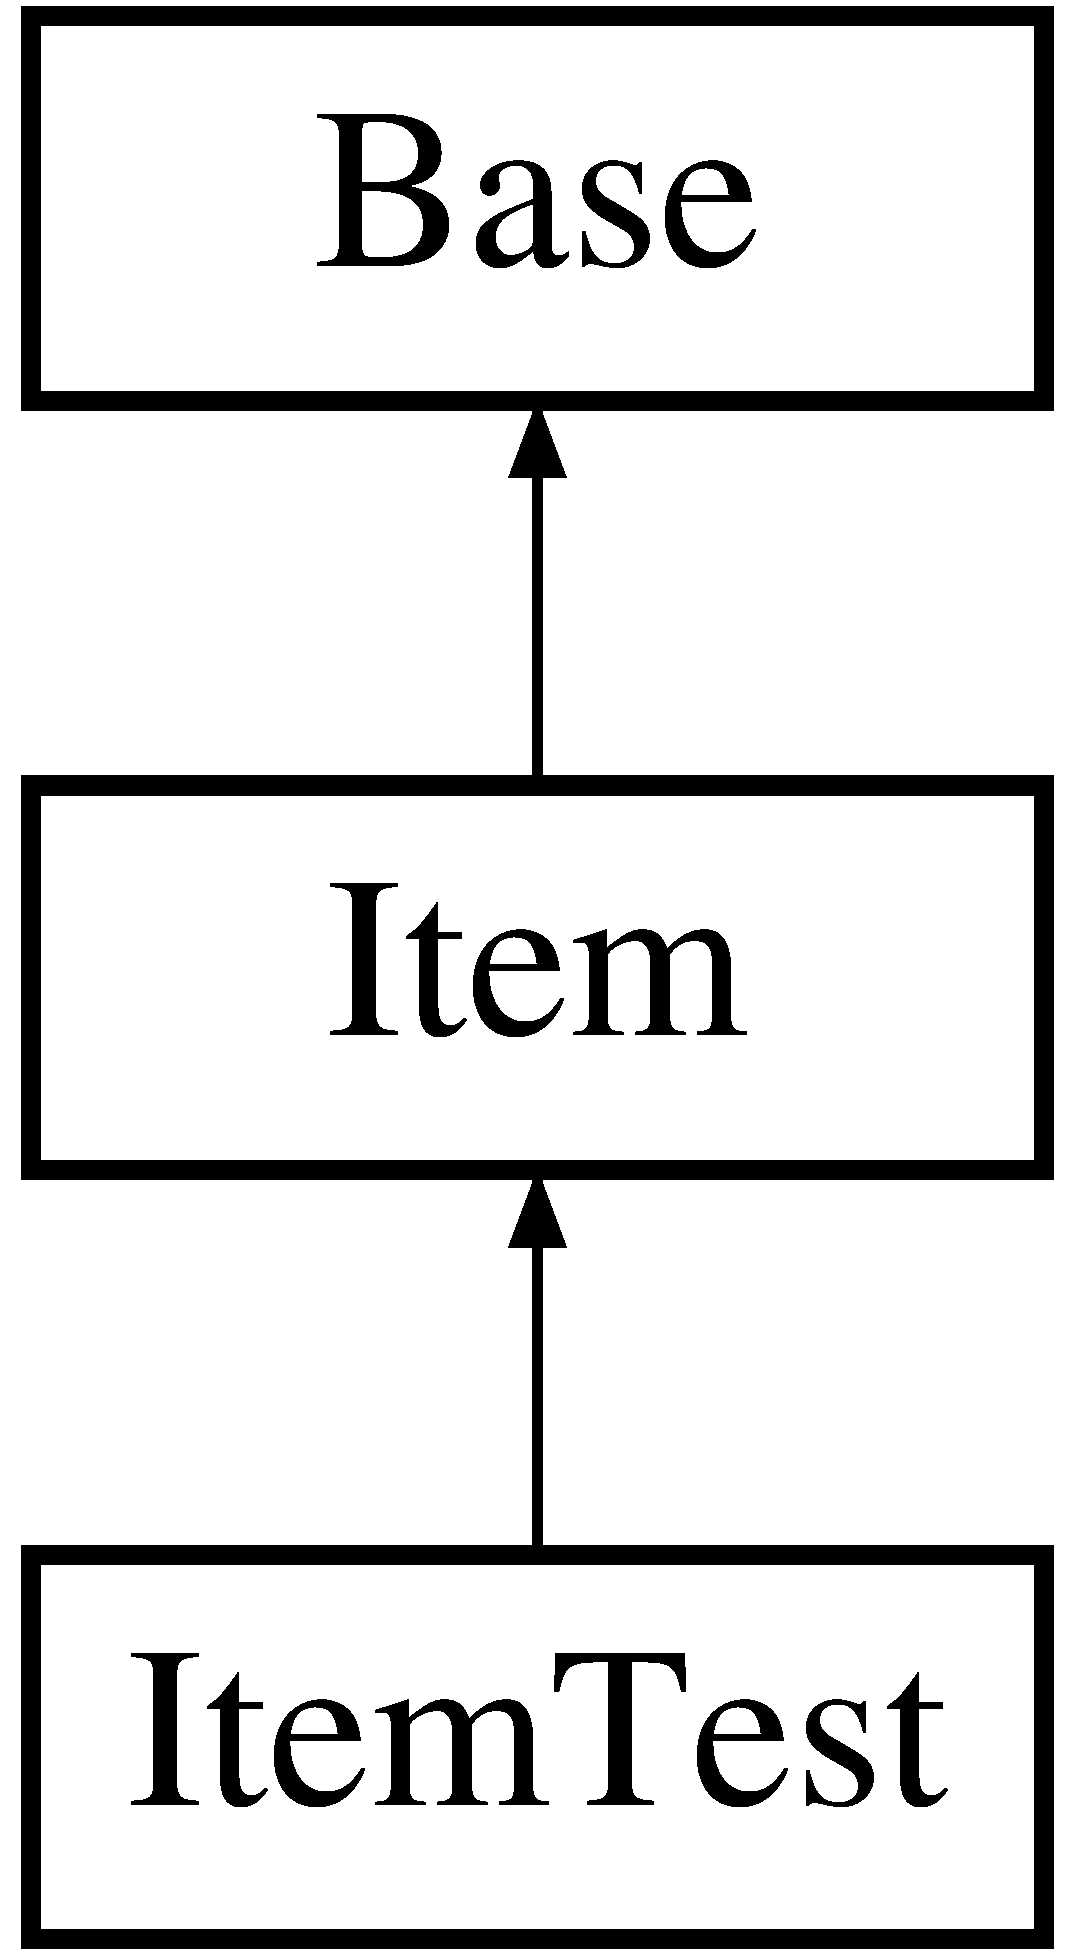
\includegraphics[height=3.000000cm]{structItemTest}
\end{center}
\end{figure}
\subsection*{Public Member Functions}
\begin{DoxyCompactItemize}
\item 
\hyperlink{structItemTest_a310a8cf4a45615e897a3f3cceefc03e8}{Item\-Test} ()
\item 
bool \hyperlink{structItemTest_a75e6ddccebab853a259a0957c15407e1}{interact} (\hyperlink{classPerson}{Person} \&person)
\item 
bool \hyperlink{structItemTest_ad30228b68d1b22411270e6b304a87249}{place} (\hyperlink{classPerson}{Person} \&person)
\item 
bool \hyperlink{structItemTest_a22ad8ab142e30bc5b1d45425ed1d26b5}{can\-Place} (\hyperlink{classPerson}{Person} \&person)
\item 
void \hyperlink{structItemTest_aa5a51547e6dacf11363e439222377b45}{update} (\hyperlink{classShipMaster}{Ship\-Master} \&ship)
\item 
int \hyperlink{structItemTest_a040963d27bd3bc753664ece6845f9650}{get\-Texture\-I\-D} ()
\end{DoxyCompactItemize}
\subsection*{Additional Inherited Members}


\subsection{Constructor \& Destructor Documentation}
\hypertarget{structItemTest_a310a8cf4a45615e897a3f3cceefc03e8}{\index{Item\-Test@{Item\-Test}!Item\-Test@{Item\-Test}}
\index{Item\-Test@{Item\-Test}!ItemTest@{Item\-Test}}
\subsubsection[{Item\-Test}]{\setlength{\rightskip}{0pt plus 5cm}Item\-Test\-::\-Item\-Test (
\begin{DoxyParamCaption}
{}
\end{DoxyParamCaption}
)\hspace{0.3cm}{\ttfamily [inline]}}}\label{structItemTest_a310a8cf4a45615e897a3f3cceefc03e8}


\subsection{Member Function Documentation}
\hypertarget{structItemTest_a22ad8ab142e30bc5b1d45425ed1d26b5}{\index{Item\-Test@{Item\-Test}!can\-Place@{can\-Place}}
\index{can\-Place@{can\-Place}!ItemTest@{Item\-Test}}
\subsubsection[{can\-Place}]{\setlength{\rightskip}{0pt plus 5cm}bool Item\-Test\-::can\-Place (
\begin{DoxyParamCaption}
\item[{{\bf Person} \&}]{person}
\end{DoxyParamCaption}
)\hspace{0.3cm}{\ttfamily [inline]}, {\ttfamily [virtual]}}}\label{structItemTest_a22ad8ab142e30bc5b1d45425ed1d26b5}


Implements \hyperlink{classItem_afa9967b10984b1886ed6097eab7239e3}{Item}.

\hypertarget{structItemTest_a040963d27bd3bc753664ece6845f9650}{\index{Item\-Test@{Item\-Test}!get\-Texture\-I\-D@{get\-Texture\-I\-D}}
\index{get\-Texture\-I\-D@{get\-Texture\-I\-D}!ItemTest@{Item\-Test}}
\subsubsection[{get\-Texture\-I\-D}]{\setlength{\rightskip}{0pt plus 5cm}int Item\-Test\-::get\-Texture\-I\-D (
\begin{DoxyParamCaption}
{}
\end{DoxyParamCaption}
)\hspace{0.3cm}{\ttfamily [inline]}, {\ttfamily [virtual]}}}\label{structItemTest_a040963d27bd3bc753664ece6845f9650}


Implements \hyperlink{classItem_a38889163e99a1f5ec9b811b8e64fbc36}{Item}.

\hypertarget{structItemTest_a75e6ddccebab853a259a0957c15407e1}{\index{Item\-Test@{Item\-Test}!interact@{interact}}
\index{interact@{interact}!ItemTest@{Item\-Test}}
\subsubsection[{interact}]{\setlength{\rightskip}{0pt plus 5cm}bool Item\-Test\-::interact (
\begin{DoxyParamCaption}
\item[{{\bf Person} \&}]{person}
\end{DoxyParamCaption}
)\hspace{0.3cm}{\ttfamily [inline]}, {\ttfamily [virtual]}}}\label{structItemTest_a75e6ddccebab853a259a0957c15407e1}


Implements \hyperlink{classItem_a65a4d68109b4aa82c62d262ab4786145}{Item}.

\hypertarget{structItemTest_ad30228b68d1b22411270e6b304a87249}{\index{Item\-Test@{Item\-Test}!place@{place}}
\index{place@{place}!ItemTest@{Item\-Test}}
\subsubsection[{place}]{\setlength{\rightskip}{0pt plus 5cm}bool Item\-Test\-::place (
\begin{DoxyParamCaption}
\item[{{\bf Person} \&}]{person}
\end{DoxyParamCaption}
)\hspace{0.3cm}{\ttfamily [inline]}, {\ttfamily [virtual]}}}\label{structItemTest_ad30228b68d1b22411270e6b304a87249}


Implements \hyperlink{classItem_a2fc04b2fdd729977c419e0a1c5c8fa87}{Item}.

\hypertarget{structItemTest_aa5a51547e6dacf11363e439222377b45}{\index{Item\-Test@{Item\-Test}!update@{update}}
\index{update@{update}!ItemTest@{Item\-Test}}
\subsubsection[{update}]{\setlength{\rightskip}{0pt plus 5cm}void Item\-Test\-::update (
\begin{DoxyParamCaption}
\item[{{\bf Ship\-Master} \&}]{ship}
\end{DoxyParamCaption}
)\hspace{0.3cm}{\ttfamily [inline]}, {\ttfamily [virtual]}}}\label{structItemTest_aa5a51547e6dacf11363e439222377b45}


Implements \hyperlink{classItem_af7cb35b77955c00a38fc0f952da762f4}{Item}.



The documentation for this struct was generated from the following file\-:\begin{DoxyCompactItemize}
\item 
core/items/\hyperlink{Item_8h}{Item.\-h}\end{DoxyCompactItemize}

\hypertarget{classJob}{\section{Job Class Reference}
\label{classJob}\index{Job@{Job}}
}


{\ttfamily \#include $<$Job.\-h$>$}

Inheritance diagram for Job\-:\begin{figure}[H]
\begin{center}
\leavevmode
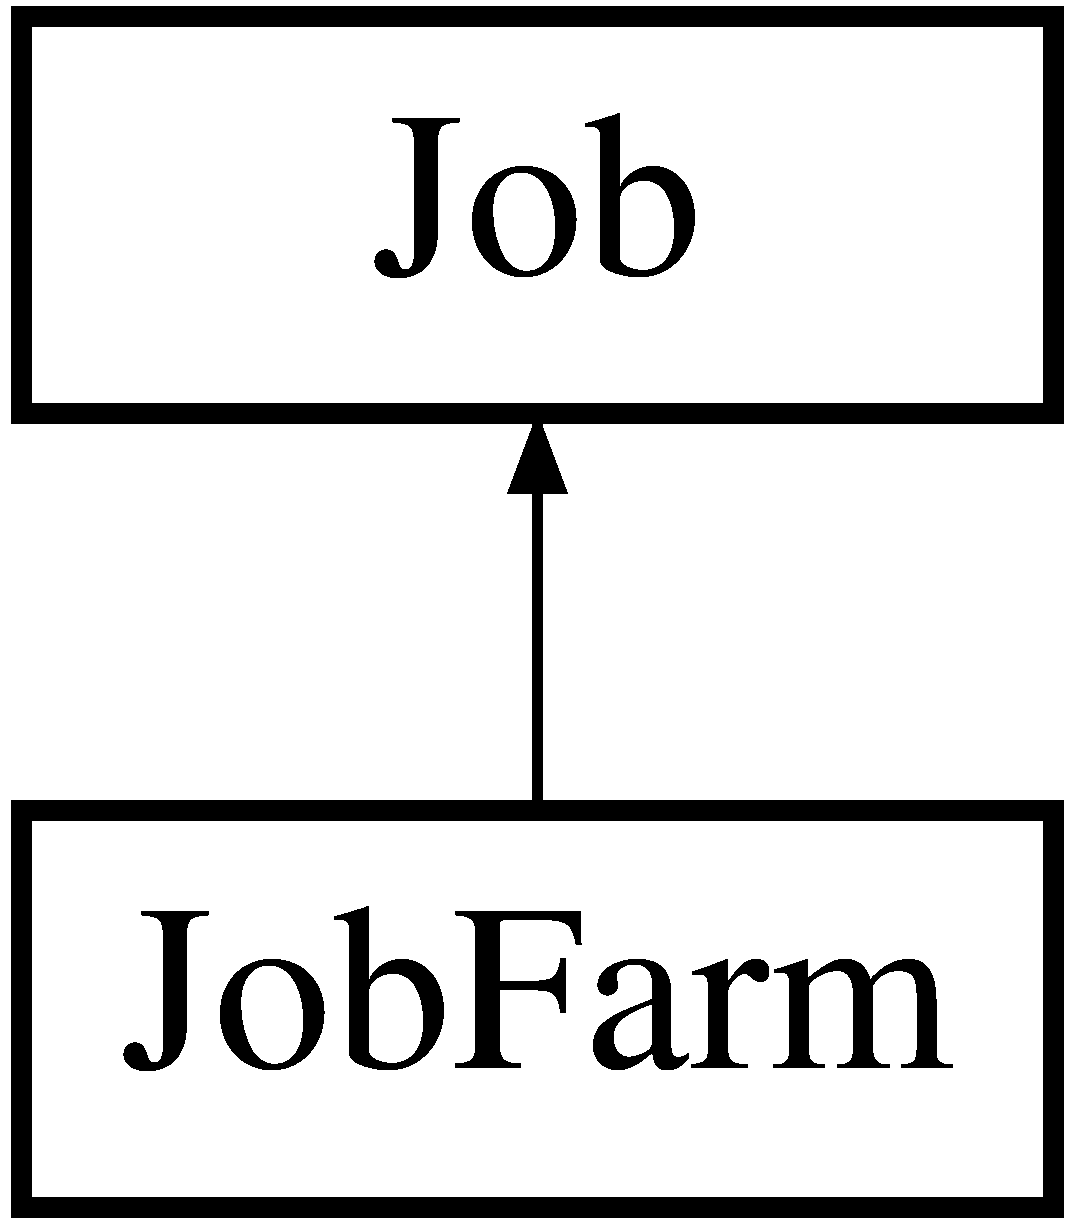
\includegraphics[height=2.000000cm]{classJob}
\end{center}
\end{figure}
\subsection*{Public Member Functions}
\begin{DoxyCompactItemize}
\item 
\hyperlink{classJob_a8929b57c85aabbd16ef7d763b155a4d4}{Job} (\hyperlink{classShipMaster}{Ship\-Master} \&\hyperlink{classJob_a728d3562b81cde6fbf5217c2ad002359}{ship})
\item 
virtual \hyperlink{classJob_ab1eef87bf28ea5930582e26faea83269}{$\sim$\-Job} ()
\item 
void \hyperlink{classJob_aa03d408ece696fa802e833b37b315742}{set\-Ship\-Master} (\hyperlink{classShipMaster}{Ship\-Master} \&\hyperlink{classJob_a728d3562b81cde6fbf5217c2ad002359}{ship})
\item 
virtual bool \hyperlink{classJob_a46715fd9c16a0c9855132d7a1925b0c4}{deligate\-Task} (\hyperlink{classPerson}{Person} \&person)=0
\end{DoxyCompactItemize}
\subsection*{Public Attributes}
\begin{DoxyCompactItemize}
\item 
\hyperlink{classShipMaster}{Ship\-Master} \& \hyperlink{classJob_a728d3562b81cde6fbf5217c2ad002359}{ship}
\end{DoxyCompactItemize}


\subsection{Constructor \& Destructor Documentation}
\hypertarget{classJob_a8929b57c85aabbd16ef7d763b155a4d4}{\index{Job@{Job}!Job@{Job}}
\index{Job@{Job}!Job@{Job}}
\subsubsection[{Job}]{\setlength{\rightskip}{0pt plus 5cm}Job\-::\-Job (
\begin{DoxyParamCaption}
\item[{{\bf Ship\-Master} \&}]{ship}
\end{DoxyParamCaption}
)}}\label{classJob_a8929b57c85aabbd16ef7d763b155a4d4}
\hypertarget{classJob_ab1eef87bf28ea5930582e26faea83269}{\index{Job@{Job}!$\sim$\-Job@{$\sim$\-Job}}
\index{$\sim$\-Job@{$\sim$\-Job}!Job@{Job}}
\subsubsection[{$\sim$\-Job}]{\setlength{\rightskip}{0pt plus 5cm}virtual Job\-::$\sim$\-Job (
\begin{DoxyParamCaption}
{}
\end{DoxyParamCaption}
)\hspace{0.3cm}{\ttfamily [inline]}, {\ttfamily [virtual]}}}\label{classJob_ab1eef87bf28ea5930582e26faea83269}


\subsection{Member Function Documentation}
\hypertarget{classJob_a46715fd9c16a0c9855132d7a1925b0c4}{\index{Job@{Job}!deligate\-Task@{deligate\-Task}}
\index{deligate\-Task@{deligate\-Task}!Job@{Job}}
\subsubsection[{deligate\-Task}]{\setlength{\rightskip}{0pt plus 5cm}virtual bool Job\-::deligate\-Task (
\begin{DoxyParamCaption}
\item[{{\bf Person} \&}]{person}
\end{DoxyParamCaption}
)\hspace{0.3cm}{\ttfamily [pure virtual]}}}\label{classJob_a46715fd9c16a0c9855132d7a1925b0c4}


Implemented in \hyperlink{classJobFarm_a9475d189e9d4e7dc86d5833e74b6a58d}{Job\-Farm}.

\hypertarget{classJob_aa03d408ece696fa802e833b37b315742}{\index{Job@{Job}!set\-Ship\-Master@{set\-Ship\-Master}}
\index{set\-Ship\-Master@{set\-Ship\-Master}!Job@{Job}}
\subsubsection[{set\-Ship\-Master}]{\setlength{\rightskip}{0pt plus 5cm}void Job\-::set\-Ship\-Master (
\begin{DoxyParamCaption}
\item[{{\bf Ship\-Master} \&}]{ship}
\end{DoxyParamCaption}
)}}\label{classJob_aa03d408ece696fa802e833b37b315742}


\subsection{Member Data Documentation}
\hypertarget{classJob_a728d3562b81cde6fbf5217c2ad002359}{\index{Job@{Job}!ship@{ship}}
\index{ship@{ship}!Job@{Job}}
\subsubsection[{ship}]{\setlength{\rightskip}{0pt plus 5cm}{\bf Ship\-Master}\& Job\-::ship}}\label{classJob_a728d3562b81cde6fbf5217c2ad002359}


The documentation for this class was generated from the following files\-:\begin{DoxyCompactItemize}
\item 
core/jobs/\hyperlink{Job_8h}{Job.\-h}\item 
core/jobs/\hyperlink{Job_8cpp}{Job.\-cpp}\end{DoxyCompactItemize}

\hypertarget{classJobFarm}{\section{Job\-Farm Class Reference}
\label{classJobFarm}\index{Job\-Farm@{Job\-Farm}}
}


{\ttfamily \#include $<$Job\-Farm.\-h$>$}

Inheritance diagram for Job\-Farm\-:\begin{figure}[H]
\begin{center}
\leavevmode
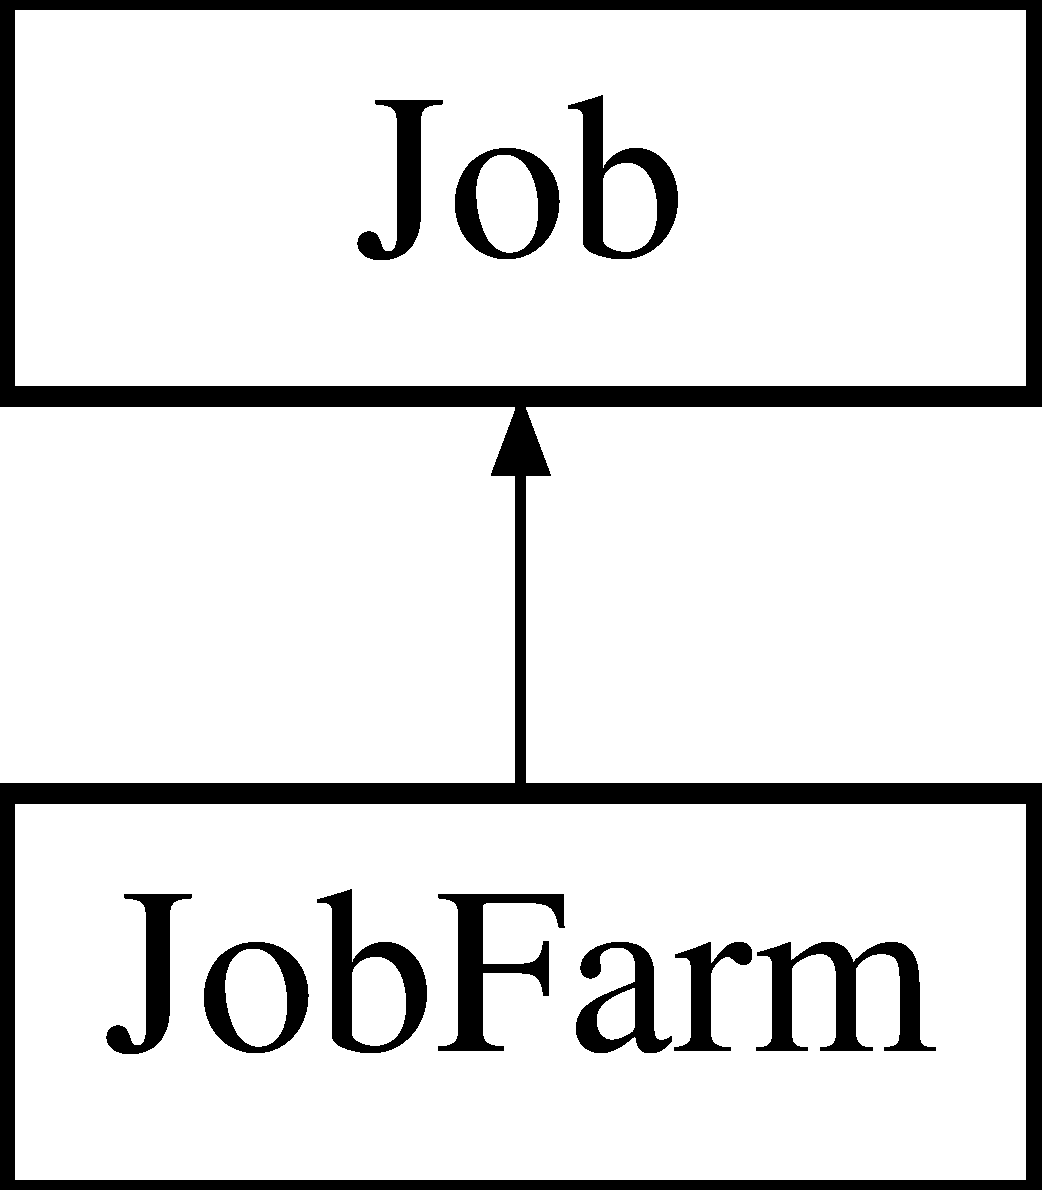
\includegraphics[height=2.000000cm]{classJobFarm}
\end{center}
\end{figure}
\subsection*{Public Member Functions}
\begin{DoxyCompactItemize}
\item 
\hyperlink{classJobFarm_a89aa0fdf534fcb44d4174d81b78b2fb3}{Job\-Farm} (\hyperlink{classShipMaster}{Ship\-Master} \&\hyperlink{classJob_a728d3562b81cde6fbf5217c2ad002359}{ship})
\item 
bool \hyperlink{classJobFarm_a9475d189e9d4e7dc86d5833e74b6a58d}{deligate\-Task} (\hyperlink{classPerson}{Person} \&person)
\item 
bool \hyperlink{classJobFarm_a0cd80871d36c25083c07238115921d17}{gather} (\hyperlink{classPerson}{Person} \&person)
\item 
bool \hyperlink{classJobFarm_ae8b519a68bc3213bd07481bbd26e034e}{sow} (\hyperlink{classPerson}{Person} \&person)
\item 
bool \hyperlink{classJobFarm_a6ed344d38f7ea5e7723e4742fff0fdf2}{has\-Seeds} (\hyperlink{classPerson}{Person} \&person)
\item 
bool \hyperlink{classJobFarm_a460c287b1516e5f78d6ab777e8d217f3}{grown\-Crops} ()
\end{DoxyCompactItemize}
\subsection*{Additional Inherited Members}


\subsection{Constructor \& Destructor Documentation}
\hypertarget{classJobFarm_a89aa0fdf534fcb44d4174d81b78b2fb3}{\index{Job\-Farm@{Job\-Farm}!Job\-Farm@{Job\-Farm}}
\index{Job\-Farm@{Job\-Farm}!JobFarm@{Job\-Farm}}
\subsubsection[{Job\-Farm}]{\setlength{\rightskip}{0pt plus 5cm}Job\-Farm\-::\-Job\-Farm (
\begin{DoxyParamCaption}
\item[{{\bf Ship\-Master} \&}]{ship}
\end{DoxyParamCaption}
)}}\label{classJobFarm_a89aa0fdf534fcb44d4174d81b78b2fb3}


\subsection{Member Function Documentation}
\hypertarget{classJobFarm_a9475d189e9d4e7dc86d5833e74b6a58d}{\index{Job\-Farm@{Job\-Farm}!deligate\-Task@{deligate\-Task}}
\index{deligate\-Task@{deligate\-Task}!JobFarm@{Job\-Farm}}
\subsubsection[{deligate\-Task}]{\setlength{\rightskip}{0pt plus 5cm}bool Job\-Farm\-::deligate\-Task (
\begin{DoxyParamCaption}
\item[{{\bf Person} \&}]{person}
\end{DoxyParamCaption}
)\hspace{0.3cm}{\ttfamily [virtual]}}}\label{classJobFarm_a9475d189e9d4e7dc86d5833e74b6a58d}


Implements \hyperlink{classJob_a46715fd9c16a0c9855132d7a1925b0c4}{Job}.

\hypertarget{classJobFarm_a0cd80871d36c25083c07238115921d17}{\index{Job\-Farm@{Job\-Farm}!gather@{gather}}
\index{gather@{gather}!JobFarm@{Job\-Farm}}
\subsubsection[{gather}]{\setlength{\rightskip}{0pt plus 5cm}bool Job\-Farm\-::gather (
\begin{DoxyParamCaption}
\item[{{\bf Person} \&}]{person}
\end{DoxyParamCaption}
)}}\label{classJobFarm_a0cd80871d36c25083c07238115921d17}
\hypertarget{classJobFarm_a460c287b1516e5f78d6ab777e8d217f3}{\index{Job\-Farm@{Job\-Farm}!grown\-Crops@{grown\-Crops}}
\index{grown\-Crops@{grown\-Crops}!JobFarm@{Job\-Farm}}
\subsubsection[{grown\-Crops}]{\setlength{\rightskip}{0pt plus 5cm}bool Job\-Farm\-::grown\-Crops (
\begin{DoxyParamCaption}
{}
\end{DoxyParamCaption}
)}}\label{classJobFarm_a460c287b1516e5f78d6ab777e8d217f3}
\hypertarget{classJobFarm_a6ed344d38f7ea5e7723e4742fff0fdf2}{\index{Job\-Farm@{Job\-Farm}!has\-Seeds@{has\-Seeds}}
\index{has\-Seeds@{has\-Seeds}!JobFarm@{Job\-Farm}}
\subsubsection[{has\-Seeds}]{\setlength{\rightskip}{0pt plus 5cm}bool Job\-Farm\-::has\-Seeds (
\begin{DoxyParamCaption}
\item[{{\bf Person} \&}]{person}
\end{DoxyParamCaption}
)}}\label{classJobFarm_a6ed344d38f7ea5e7723e4742fff0fdf2}
\hypertarget{classJobFarm_ae8b519a68bc3213bd07481bbd26e034e}{\index{Job\-Farm@{Job\-Farm}!sow@{sow}}
\index{sow@{sow}!JobFarm@{Job\-Farm}}
\subsubsection[{sow}]{\setlength{\rightskip}{0pt plus 5cm}bool Job\-Farm\-::sow (
\begin{DoxyParamCaption}
\item[{{\bf Person} \&}]{person}
\end{DoxyParamCaption}
)}}\label{classJobFarm_ae8b519a68bc3213bd07481bbd26e034e}


The documentation for this class was generated from the following files\-:\begin{DoxyCompactItemize}
\item 
core/jobs/\hyperlink{JobFarm_8h}{Job\-Farm.\-h}\item 
core/jobs/\hyperlink{JobFarm_8cpp}{Job\-Farm.\-cpp}\end{DoxyCompactItemize}

\hypertarget{classLinkedList}{\section{Linked\-List Class Reference}
\label{classLinkedList}\index{Linked\-List@{Linked\-List}}
}


{\ttfamily \#include $<$Linked\-List.\-h$>$}

\subsection*{Public Member Functions}
\begin{DoxyCompactItemize}
\item 
\hyperlink{classLinkedList_afe7f78983e173f8018927cf2ad11a5aa}{Linked\-List} ()
\item 
\hyperlink{classLinkedList_a35811ed58ff0d8d9cc9b309b8d8f5111}{$\sim$\-Linked\-List} ()
\item 
void \hyperlink{classLinkedList_a78172a81bf60fbbd33e65305826d028b}{add} (\hyperlink{classItem}{Item} $\ast$val)
\item 
bool \hyperlink{classLinkedList_a03ff22f881325da2d37f640ab2380bf2}{is\-Empty} ()
\item 
int \hyperlink{classLinkedList_a92bb5271734b51ab089d75bf52aee919}{get\-Length} ()
\item 
void \hyperlink{classLinkedList_ae973d79346684a26166c539896d2d1b7}{update} (\hyperlink{classShipMaster}{Ship\-Master} \&ship)
\item 
void \hyperlink{classLinkedList_a261977565e78dd74f288d47ba5865242}{clear} ()
\item 
\hyperlink{classItem}{Item} $\ast$ \hyperlink{classLinkedList_a52c070ab08f67e26ec260412024fb20e}{find\-With\-U\-I\-D} (int U\-I\-D)
\item 
\hyperlink{classItem}{Item} $\ast$ \hyperlink{classLinkedList_ae051024e7e6ba32002ba0f40a7843f0d}{find\-With\-I\-D} (int I\-D)
\item 
\hyperlink{classItem}{Item} $\ast$ \hyperlink{classLinkedList_ab7bc50ad1c97b0559d00e5a6e2da78cd}{find\-With\-Index} (int i)
\item 
\hyperlink{classItem}{Item} $\ast$ \hyperlink{classLinkedList_abfe92bb8d0e4ab6072a09a74a515111e}{pop\-With\-U\-I\-D} (int U\-I\-D)
\item 
\hyperlink{classItem}{Item} $\ast$ \hyperlink{classLinkedList_a181a5fd6df446be45690966536aaf3c6}{pop\-With\-I\-D} (int I\-D)
\item 
\hyperlink{classItem}{Item} $\ast$ \hyperlink{classLinkedList_a30b300a0ad095ac7c19717cb3894ddb2}{pop} ()
\item 
\hyperlink{classItem}{Item} $\ast$ \hyperlink{classLinkedList_a7106d9f9335485f9f4bc6945d25d9804}{next} ()
\item 
void \hyperlink{classLinkedList_aa97c4254d7eacee2b33ce306c3162b61}{reset\-Iterator} ()
\end{DoxyCompactItemize}


\subsection{Constructor \& Destructor Documentation}
\hypertarget{classLinkedList_afe7f78983e173f8018927cf2ad11a5aa}{\index{Linked\-List@{Linked\-List}!Linked\-List@{Linked\-List}}
\index{Linked\-List@{Linked\-List}!LinkedList@{Linked\-List}}
\subsubsection[{Linked\-List}]{\setlength{\rightskip}{0pt plus 5cm}Linked\-List\-::\-Linked\-List (
\begin{DoxyParamCaption}
{}
\end{DoxyParamCaption}
)}}\label{classLinkedList_afe7f78983e173f8018927cf2ad11a5aa}
\hypertarget{classLinkedList_a35811ed58ff0d8d9cc9b309b8d8f5111}{\index{Linked\-List@{Linked\-List}!$\sim$\-Linked\-List@{$\sim$\-Linked\-List}}
\index{$\sim$\-Linked\-List@{$\sim$\-Linked\-List}!LinkedList@{Linked\-List}}
\subsubsection[{$\sim$\-Linked\-List}]{\setlength{\rightskip}{0pt plus 5cm}Linked\-List\-::$\sim$\-Linked\-List (
\begin{DoxyParamCaption}
{}
\end{DoxyParamCaption}
)}}\label{classLinkedList_a35811ed58ff0d8d9cc9b309b8d8f5111}


\subsection{Member Function Documentation}
\hypertarget{classLinkedList_a78172a81bf60fbbd33e65305826d028b}{\index{Linked\-List@{Linked\-List}!add@{add}}
\index{add@{add}!LinkedList@{Linked\-List}}
\subsubsection[{add}]{\setlength{\rightskip}{0pt plus 5cm}void Linked\-List\-::add (
\begin{DoxyParamCaption}
\item[{{\bf Item} $\ast$}]{val}
\end{DoxyParamCaption}
)}}\label{classLinkedList_a78172a81bf60fbbd33e65305826d028b}
\hypertarget{classLinkedList_a261977565e78dd74f288d47ba5865242}{\index{Linked\-List@{Linked\-List}!clear@{clear}}
\index{clear@{clear}!LinkedList@{Linked\-List}}
\subsubsection[{clear}]{\setlength{\rightskip}{0pt plus 5cm}void Linked\-List\-::clear (
\begin{DoxyParamCaption}
{}
\end{DoxyParamCaption}
)}}\label{classLinkedList_a261977565e78dd74f288d47ba5865242}
\hypertarget{classLinkedList_ae051024e7e6ba32002ba0f40a7843f0d}{\index{Linked\-List@{Linked\-List}!find\-With\-I\-D@{find\-With\-I\-D}}
\index{find\-With\-I\-D@{find\-With\-I\-D}!LinkedList@{Linked\-List}}
\subsubsection[{find\-With\-I\-D}]{\setlength{\rightskip}{0pt plus 5cm}{\bf Item} $\ast$ Linked\-List\-::find\-With\-I\-D (
\begin{DoxyParamCaption}
\item[{int}]{I\-D}
\end{DoxyParamCaption}
)}}\label{classLinkedList_ae051024e7e6ba32002ba0f40a7843f0d}
\hypertarget{classLinkedList_ab7bc50ad1c97b0559d00e5a6e2da78cd}{\index{Linked\-List@{Linked\-List}!find\-With\-Index@{find\-With\-Index}}
\index{find\-With\-Index@{find\-With\-Index}!LinkedList@{Linked\-List}}
\subsubsection[{find\-With\-Index}]{\setlength{\rightskip}{0pt plus 5cm}{\bf Item} $\ast$ Linked\-List\-::find\-With\-Index (
\begin{DoxyParamCaption}
\item[{int}]{i}
\end{DoxyParamCaption}
)}}\label{classLinkedList_ab7bc50ad1c97b0559d00e5a6e2da78cd}
\hypertarget{classLinkedList_a52c070ab08f67e26ec260412024fb20e}{\index{Linked\-List@{Linked\-List}!find\-With\-U\-I\-D@{find\-With\-U\-I\-D}}
\index{find\-With\-U\-I\-D@{find\-With\-U\-I\-D}!LinkedList@{Linked\-List}}
\subsubsection[{find\-With\-U\-I\-D}]{\setlength{\rightskip}{0pt plus 5cm}{\bf Item} $\ast$ Linked\-List\-::find\-With\-U\-I\-D (
\begin{DoxyParamCaption}
\item[{int}]{U\-I\-D}
\end{DoxyParamCaption}
)}}\label{classLinkedList_a52c070ab08f67e26ec260412024fb20e}
\hypertarget{classLinkedList_a92bb5271734b51ab089d75bf52aee919}{\index{Linked\-List@{Linked\-List}!get\-Length@{get\-Length}}
\index{get\-Length@{get\-Length}!LinkedList@{Linked\-List}}
\subsubsection[{get\-Length}]{\setlength{\rightskip}{0pt plus 5cm}int Linked\-List\-::get\-Length (
\begin{DoxyParamCaption}
{}
\end{DoxyParamCaption}
)}}\label{classLinkedList_a92bb5271734b51ab089d75bf52aee919}
\hypertarget{classLinkedList_a03ff22f881325da2d37f640ab2380bf2}{\index{Linked\-List@{Linked\-List}!is\-Empty@{is\-Empty}}
\index{is\-Empty@{is\-Empty}!LinkedList@{Linked\-List}}
\subsubsection[{is\-Empty}]{\setlength{\rightskip}{0pt plus 5cm}bool Linked\-List\-::is\-Empty (
\begin{DoxyParamCaption}
{}
\end{DoxyParamCaption}
)}}\label{classLinkedList_a03ff22f881325da2d37f640ab2380bf2}
\hypertarget{classLinkedList_a7106d9f9335485f9f4bc6945d25d9804}{\index{Linked\-List@{Linked\-List}!next@{next}}
\index{next@{next}!LinkedList@{Linked\-List}}
\subsubsection[{next}]{\setlength{\rightskip}{0pt plus 5cm}{\bf Item} $\ast$ Linked\-List\-::next (
\begin{DoxyParamCaption}
{}
\end{DoxyParamCaption}
)}}\label{classLinkedList_a7106d9f9335485f9f4bc6945d25d9804}
\hypertarget{classLinkedList_a30b300a0ad095ac7c19717cb3894ddb2}{\index{Linked\-List@{Linked\-List}!pop@{pop}}
\index{pop@{pop}!LinkedList@{Linked\-List}}
\subsubsection[{pop}]{\setlength{\rightskip}{0pt plus 5cm}{\bf Item} $\ast$ Linked\-List\-::pop (
\begin{DoxyParamCaption}
{}
\end{DoxyParamCaption}
)}}\label{classLinkedList_a30b300a0ad095ac7c19717cb3894ddb2}
\hypertarget{classLinkedList_a181a5fd6df446be45690966536aaf3c6}{\index{Linked\-List@{Linked\-List}!pop\-With\-I\-D@{pop\-With\-I\-D}}
\index{pop\-With\-I\-D@{pop\-With\-I\-D}!LinkedList@{Linked\-List}}
\subsubsection[{pop\-With\-I\-D}]{\setlength{\rightskip}{0pt plus 5cm}{\bf Item} $\ast$ Linked\-List\-::pop\-With\-I\-D (
\begin{DoxyParamCaption}
\item[{int}]{I\-D}
\end{DoxyParamCaption}
)}}\label{classLinkedList_a181a5fd6df446be45690966536aaf3c6}
\hypertarget{classLinkedList_abfe92bb8d0e4ab6072a09a74a515111e}{\index{Linked\-List@{Linked\-List}!pop\-With\-U\-I\-D@{pop\-With\-U\-I\-D}}
\index{pop\-With\-U\-I\-D@{pop\-With\-U\-I\-D}!LinkedList@{Linked\-List}}
\subsubsection[{pop\-With\-U\-I\-D}]{\setlength{\rightskip}{0pt plus 5cm}{\bf Item} $\ast$ Linked\-List\-::pop\-With\-U\-I\-D (
\begin{DoxyParamCaption}
\item[{int}]{U\-I\-D}
\end{DoxyParamCaption}
)}}\label{classLinkedList_abfe92bb8d0e4ab6072a09a74a515111e}
\hypertarget{classLinkedList_aa97c4254d7eacee2b33ce306c3162b61}{\index{Linked\-List@{Linked\-List}!reset\-Iterator@{reset\-Iterator}}
\index{reset\-Iterator@{reset\-Iterator}!LinkedList@{Linked\-List}}
\subsubsection[{reset\-Iterator}]{\setlength{\rightskip}{0pt plus 5cm}void Linked\-List\-::reset\-Iterator (
\begin{DoxyParamCaption}
{}
\end{DoxyParamCaption}
)}}\label{classLinkedList_aa97c4254d7eacee2b33ce306c3162b61}
\hypertarget{classLinkedList_ae973d79346684a26166c539896d2d1b7}{\index{Linked\-List@{Linked\-List}!update@{update}}
\index{update@{update}!LinkedList@{Linked\-List}}
\subsubsection[{update}]{\setlength{\rightskip}{0pt plus 5cm}void Linked\-List\-::update (
\begin{DoxyParamCaption}
\item[{{\bf Ship\-Master} \&}]{ship}
\end{DoxyParamCaption}
)}}\label{classLinkedList_ae973d79346684a26166c539896d2d1b7}


The documentation for this class was generated from the following files\-:\begin{DoxyCompactItemize}
\item 
core/items/\hyperlink{LinkedList_8h}{Linked\-List.\-h}\item 
core/items/\hyperlink{LinkedList_8cpp}{Linked\-List.\-cpp}\end{DoxyCompactItemize}

\hypertarget{structLocation}{\section{Location Struct Reference}
\label{structLocation}\index{Location@{Location}}
}


Custom, simple location class.  




{\ttfamily \#include $<$Location.\-h$>$}

\subsection*{Public Member Functions}
\begin{DoxyCompactItemize}
\item 
\hyperlink{structLocation_a87790c14997fd8cdd12080c78c9794bb}{Location} ()
\item 
\hyperlink{structLocation_a02b70305fcef2e7913e5282bbafe7833}{Location} (const \hyperlink{structLocation}{Location} \&obj)
\item 
\hyperlink{structLocation_ada7ef731cfa1f39a6512b3e6eecf434d}{Location} (int \hyperlink{structLocation_aea76eebc474e30c04c53e5f03c6749e3}{x}, int \hyperlink{structLocation_a307809776b981810147af56d9304e273}{y}, int \hyperlink{structLocation_ad46e606795ee67a3775a53da49b37284}{z})
\item 
\hyperlink{structLocation}{Location} \& \hyperlink{structLocation_a4872cfb218bcb4c430a020f9e152866a}{operator=} (const \hyperlink{structLocation}{Location} \&obj)
\item 
void \hyperlink{structLocation_a4779c67a789befcb983db6d815ae9812}{copy} (const \hyperlink{structLocation}{Location} \&obj)
\end{DoxyCompactItemize}
\subsection*{Public Attributes}
\begin{DoxyCompactItemize}
\item 
int \hyperlink{structLocation_aea76eebc474e30c04c53e5f03c6749e3}{x}
\item 
int \hyperlink{structLocation_a307809776b981810147af56d9304e273}{y}
\item 
int \hyperlink{structLocation_ad46e606795ee67a3775a53da49b37284}{z}
\end{DoxyCompactItemize}


\subsection{Detailed Description}
Custom, simple location class. 

\subsection{Constructor \& Destructor Documentation}
\hypertarget{structLocation_a87790c14997fd8cdd12080c78c9794bb}{\index{Location@{Location}!Location@{Location}}
\index{Location@{Location}!Location@{Location}}
\subsubsection[{Location}]{\setlength{\rightskip}{0pt plus 5cm}Location\-::\-Location (
\begin{DoxyParamCaption}
{}
\end{DoxyParamCaption}
)\hspace{0.3cm}{\ttfamily [inline]}}}\label{structLocation_a87790c14997fd8cdd12080c78c9794bb}
\hypertarget{structLocation_a02b70305fcef2e7913e5282bbafe7833}{\index{Location@{Location}!Location@{Location}}
\index{Location@{Location}!Location@{Location}}
\subsubsection[{Location}]{\setlength{\rightskip}{0pt plus 5cm}Location\-::\-Location (
\begin{DoxyParamCaption}
\item[{const {\bf Location} \&}]{obj}
\end{DoxyParamCaption}
)\hspace{0.3cm}{\ttfamily [inline]}}}\label{structLocation_a02b70305fcef2e7913e5282bbafe7833}
\hypertarget{structLocation_ada7ef731cfa1f39a6512b3e6eecf434d}{\index{Location@{Location}!Location@{Location}}
\index{Location@{Location}!Location@{Location}}
\subsubsection[{Location}]{\setlength{\rightskip}{0pt plus 5cm}Location\-::\-Location (
\begin{DoxyParamCaption}
\item[{int}]{x, }
\item[{int}]{y, }
\item[{int}]{z}
\end{DoxyParamCaption}
)\hspace{0.3cm}{\ttfamily [inline]}}}\label{structLocation_ada7ef731cfa1f39a6512b3e6eecf434d}


\subsection{Member Function Documentation}
\hypertarget{structLocation_a4779c67a789befcb983db6d815ae9812}{\index{Location@{Location}!copy@{copy}}
\index{copy@{copy}!Location@{Location}}
\subsubsection[{copy}]{\setlength{\rightskip}{0pt plus 5cm}void Location\-::copy (
\begin{DoxyParamCaption}
\item[{const {\bf Location} \&}]{obj}
\end{DoxyParamCaption}
)\hspace{0.3cm}{\ttfamily [inline]}}}\label{structLocation_a4779c67a789befcb983db6d815ae9812}
\hypertarget{structLocation_a4872cfb218bcb4c430a020f9e152866a}{\index{Location@{Location}!operator=@{operator=}}
\index{operator=@{operator=}!Location@{Location}}
\subsubsection[{operator=}]{\setlength{\rightskip}{0pt plus 5cm}{\bf Location}\& Location\-::operator= (
\begin{DoxyParamCaption}
\item[{const {\bf Location} \&}]{obj}
\end{DoxyParamCaption}
)\hspace{0.3cm}{\ttfamily [inline]}}}\label{structLocation_a4872cfb218bcb4c430a020f9e152866a}


\subsection{Member Data Documentation}
\hypertarget{structLocation_aea76eebc474e30c04c53e5f03c6749e3}{\index{Location@{Location}!x@{x}}
\index{x@{x}!Location@{Location}}
\subsubsection[{x}]{\setlength{\rightskip}{0pt plus 5cm}int Location\-::x}}\label{structLocation_aea76eebc474e30c04c53e5f03c6749e3}
\hypertarget{structLocation_a307809776b981810147af56d9304e273}{\index{Location@{Location}!y@{y}}
\index{y@{y}!Location@{Location}}
\subsubsection[{y}]{\setlength{\rightskip}{0pt plus 5cm}int Location\-::y}}\label{structLocation_a307809776b981810147af56d9304e273}
\hypertarget{structLocation_ad46e606795ee67a3775a53da49b37284}{\index{Location@{Location}!z@{z}}
\index{z@{z}!Location@{Location}}
\subsubsection[{z}]{\setlength{\rightskip}{0pt plus 5cm}int Location\-::z}}\label{structLocation_ad46e606795ee67a3775a53da49b37284}


The documentation for this struct was generated from the following file\-:\begin{DoxyCompactItemize}
\item 
core/map/\hyperlink{Location_8h}{Location.\-h}\end{DoxyCompactItemize}

\hypertarget{classMapVisualizer}{\section{Map\-Visualizer Class Reference}
\label{classMapVisualizer}\index{Map\-Visualizer@{Map\-Visualizer}}
}


{\ttfamily \#include $<$Map\-Visualizer.\-h$>$}

\subsection*{Public Member Functions}
\begin{DoxyCompactItemize}
\item 
\hyperlink{classMapVisualizer_aa19d7369375404748df5c67d87f7bea2}{Map\-Visualizer} (\hyperlink{classShipMaster}{Ship\-Master} $\ast$\hyperlink{classMapVisualizer_aae41754a661628c88a957589e48b7b9e}{ship}, T\-M\-X\-Tiled\-Map $\ast$\hyperlink{classMapVisualizer_a8178bb6206e1d4f7eded58480e43d92c}{map\-Tiled}, Layer $\ast$\hyperlink{classMapVisualizer_a7fde95f09d1c8ef52b79e6d65d7c0b0c}{scene})
\item 
\hyperlink{classMapVisualizer_a0e1710c52a3cc31b1d7a173d522dce4a}{$\sim$\-Map\-Visualizer} ()
\item 
void \hyperlink{classMapVisualizer_ae5e795271c74d55aec34319a133c271c}{update} ()
\item 
void \hyperlink{classMapVisualizer_a5185365b1153687db34722d59ee380d2}{add\-Crew\-Texture} (int amount)
\end{DoxyCompactItemize}
\subsection*{Public Attributes}
\begin{DoxyCompactItemize}
\item 
int \hyperlink{classMapVisualizer_a6e43275dd163342cea857a167c030279}{width}
\item 
int \hyperlink{classMapVisualizer_a8188730e44205bff9042b5188a8da27f}{height}
\item 
\hyperlink{classShipMaster}{Ship\-Master} $\ast$ \hyperlink{classMapVisualizer_aae41754a661628c88a957589e48b7b9e}{ship}
\item 
\hyperlink{classLinkedList}{Linked\-List} \& \hyperlink{classMapVisualizer_a73722302b4056efd5a43d633c8590b21}{items\-To\-Draw}
\item 
T\-M\-X\-Tiled\-Map $\ast$ \hyperlink{classMapVisualizer_a8178bb6206e1d4f7eded58480e43d92c}{map\-Tiled}
\item 
Layer $\ast$ \hyperlink{classMapVisualizer_a7fde95f09d1c8ef52b79e6d65d7c0b0c}{scene}
\item 
T\-M\-X\-Layer $\ast$ \hyperlink{classMapVisualizer_acb9dfe2f29396a1938df1303612b6704}{layer1}
\item 
int \hyperlink{classMapVisualizer_aee1be87aff3988b22df7af13202f3aeb}{crew\-Count}
\item 
\hyperlink{classPerson}{Person} $\ast$$\ast$ \hyperlink{classMapVisualizer_a918c6dda3581d5541f4106bfdb16e7f6}{crew}
\item 
Sprite $\ast$$\ast$ \hyperlink{classMapVisualizer_a888b3918b38bb1f9cbbf9e28478de1bb}{crew\-Sprites}
\end{DoxyCompactItemize}


\subsection{Constructor \& Destructor Documentation}
\hypertarget{classMapVisualizer_aa19d7369375404748df5c67d87f7bea2}{\index{Map\-Visualizer@{Map\-Visualizer}!Map\-Visualizer@{Map\-Visualizer}}
\index{Map\-Visualizer@{Map\-Visualizer}!MapVisualizer@{Map\-Visualizer}}
\subsubsection[{Map\-Visualizer}]{\setlength{\rightskip}{0pt plus 5cm}Map\-Visualizer\-::\-Map\-Visualizer (
\begin{DoxyParamCaption}
\item[{{\bf Ship\-Master} $\ast$}]{ship, }
\item[{T\-M\-X\-Tiled\-Map $\ast$}]{map\-Tiled, }
\item[{Layer $\ast$}]{scene}
\end{DoxyParamCaption}
)}}\label{classMapVisualizer_aa19d7369375404748df5c67d87f7bea2}
\hypertarget{classMapVisualizer_a0e1710c52a3cc31b1d7a173d522dce4a}{\index{Map\-Visualizer@{Map\-Visualizer}!$\sim$\-Map\-Visualizer@{$\sim$\-Map\-Visualizer}}
\index{$\sim$\-Map\-Visualizer@{$\sim$\-Map\-Visualizer}!MapVisualizer@{Map\-Visualizer}}
\subsubsection[{$\sim$\-Map\-Visualizer}]{\setlength{\rightskip}{0pt plus 5cm}Map\-Visualizer\-::$\sim$\-Map\-Visualizer (
\begin{DoxyParamCaption}
{}
\end{DoxyParamCaption}
)}}\label{classMapVisualizer_a0e1710c52a3cc31b1d7a173d522dce4a}


\subsection{Member Function Documentation}
\hypertarget{classMapVisualizer_a5185365b1153687db34722d59ee380d2}{\index{Map\-Visualizer@{Map\-Visualizer}!add\-Crew\-Texture@{add\-Crew\-Texture}}
\index{add\-Crew\-Texture@{add\-Crew\-Texture}!MapVisualizer@{Map\-Visualizer}}
\subsubsection[{add\-Crew\-Texture}]{\setlength{\rightskip}{0pt plus 5cm}void Map\-Visualizer\-::add\-Crew\-Texture (
\begin{DoxyParamCaption}
\item[{int}]{amount}
\end{DoxyParamCaption}
)}}\label{classMapVisualizer_a5185365b1153687db34722d59ee380d2}
\hypertarget{classMapVisualizer_ae5e795271c74d55aec34319a133c271c}{\index{Map\-Visualizer@{Map\-Visualizer}!update@{update}}
\index{update@{update}!MapVisualizer@{Map\-Visualizer}}
\subsubsection[{update}]{\setlength{\rightskip}{0pt plus 5cm}void Map\-Visualizer\-::update (
\begin{DoxyParamCaption}
{}
\end{DoxyParamCaption}
)}}\label{classMapVisualizer_ae5e795271c74d55aec34319a133c271c}


\subsection{Member Data Documentation}
\hypertarget{classMapVisualizer_a918c6dda3581d5541f4106bfdb16e7f6}{\index{Map\-Visualizer@{Map\-Visualizer}!crew@{crew}}
\index{crew@{crew}!MapVisualizer@{Map\-Visualizer}}
\subsubsection[{crew}]{\setlength{\rightskip}{0pt plus 5cm}{\bf Person}$\ast$$\ast$ Map\-Visualizer\-::crew}}\label{classMapVisualizer_a918c6dda3581d5541f4106bfdb16e7f6}
\hypertarget{classMapVisualizer_aee1be87aff3988b22df7af13202f3aeb}{\index{Map\-Visualizer@{Map\-Visualizer}!crew\-Count@{crew\-Count}}
\index{crew\-Count@{crew\-Count}!MapVisualizer@{Map\-Visualizer}}
\subsubsection[{crew\-Count}]{\setlength{\rightskip}{0pt plus 5cm}int Map\-Visualizer\-::crew\-Count}}\label{classMapVisualizer_aee1be87aff3988b22df7af13202f3aeb}
\hypertarget{classMapVisualizer_a888b3918b38bb1f9cbbf9e28478de1bb}{\index{Map\-Visualizer@{Map\-Visualizer}!crew\-Sprites@{crew\-Sprites}}
\index{crew\-Sprites@{crew\-Sprites}!MapVisualizer@{Map\-Visualizer}}
\subsubsection[{crew\-Sprites}]{\setlength{\rightskip}{0pt plus 5cm}Sprite$\ast$$\ast$ Map\-Visualizer\-::crew\-Sprites}}\label{classMapVisualizer_a888b3918b38bb1f9cbbf9e28478de1bb}
\hypertarget{classMapVisualizer_a8188730e44205bff9042b5188a8da27f}{\index{Map\-Visualizer@{Map\-Visualizer}!height@{height}}
\index{height@{height}!MapVisualizer@{Map\-Visualizer}}
\subsubsection[{height}]{\setlength{\rightskip}{0pt plus 5cm}int Map\-Visualizer\-::height}}\label{classMapVisualizer_a8188730e44205bff9042b5188a8da27f}
\hypertarget{classMapVisualizer_a73722302b4056efd5a43d633c8590b21}{\index{Map\-Visualizer@{Map\-Visualizer}!items\-To\-Draw@{items\-To\-Draw}}
\index{items\-To\-Draw@{items\-To\-Draw}!MapVisualizer@{Map\-Visualizer}}
\subsubsection[{items\-To\-Draw}]{\setlength{\rightskip}{0pt plus 5cm}{\bf Linked\-List}\& Map\-Visualizer\-::items\-To\-Draw}}\label{classMapVisualizer_a73722302b4056efd5a43d633c8590b21}
\hypertarget{classMapVisualizer_acb9dfe2f29396a1938df1303612b6704}{\index{Map\-Visualizer@{Map\-Visualizer}!layer1@{layer1}}
\index{layer1@{layer1}!MapVisualizer@{Map\-Visualizer}}
\subsubsection[{layer1}]{\setlength{\rightskip}{0pt plus 5cm}T\-M\-X\-Layer$\ast$ Map\-Visualizer\-::layer1}}\label{classMapVisualizer_acb9dfe2f29396a1938df1303612b6704}
\hypertarget{classMapVisualizer_a8178bb6206e1d4f7eded58480e43d92c}{\index{Map\-Visualizer@{Map\-Visualizer}!map\-Tiled@{map\-Tiled}}
\index{map\-Tiled@{map\-Tiled}!MapVisualizer@{Map\-Visualizer}}
\subsubsection[{map\-Tiled}]{\setlength{\rightskip}{0pt plus 5cm}T\-M\-X\-Tiled\-Map$\ast$ Map\-Visualizer\-::map\-Tiled}}\label{classMapVisualizer_a8178bb6206e1d4f7eded58480e43d92c}
\hypertarget{classMapVisualizer_a7fde95f09d1c8ef52b79e6d65d7c0b0c}{\index{Map\-Visualizer@{Map\-Visualizer}!scene@{scene}}
\index{scene@{scene}!MapVisualizer@{Map\-Visualizer}}
\subsubsection[{scene}]{\setlength{\rightskip}{0pt plus 5cm}Layer$\ast$ Map\-Visualizer\-::scene}}\label{classMapVisualizer_a7fde95f09d1c8ef52b79e6d65d7c0b0c}
\hypertarget{classMapVisualizer_aae41754a661628c88a957589e48b7b9e}{\index{Map\-Visualizer@{Map\-Visualizer}!ship@{ship}}
\index{ship@{ship}!MapVisualizer@{Map\-Visualizer}}
\subsubsection[{ship}]{\setlength{\rightskip}{0pt plus 5cm}{\bf Ship\-Master}$\ast$ Map\-Visualizer\-::ship}}\label{classMapVisualizer_aae41754a661628c88a957589e48b7b9e}
\hypertarget{classMapVisualizer_a6e43275dd163342cea857a167c030279}{\index{Map\-Visualizer@{Map\-Visualizer}!width@{width}}
\index{width@{width}!MapVisualizer@{Map\-Visualizer}}
\subsubsection[{width}]{\setlength{\rightskip}{0pt plus 5cm}int Map\-Visualizer\-::width}}\label{classMapVisualizer_a6e43275dd163342cea857a167c030279}


The documentation for this class was generated from the following files\-:\begin{DoxyCompactItemize}
\item 
\hyperlink{MapVisualizer_8h}{Map\-Visualizer.\-h}\item 
\hyperlink{MapVisualizer_8cpp}{Map\-Visualizer.\-cpp}\end{DoxyCompactItemize}

\hypertarget{classMatrix3D}{\section{Matrix3\-D Class Reference}
\label{classMatrix3D}\index{Matrix3\-D@{Matrix3\-D}}
}


{\ttfamily \#include $<$Matrix3\-D.\-h$>$}

\subsection*{Public Member Functions}
\begin{DoxyCompactItemize}
\item 
\hyperlink{classMatrix3D_afe9c6b7abe858fe9f6aea8f0607a00a7}{Matrix3\-D} ()
\item 
\hyperlink{classMatrix3D_a67ebf80ff62e71d327066491811401af}{$\sim$\-Matrix3\-D} ()
\item 
\hyperlink{classMatrix3D_a51455404cc25fe88aeaaca00ed84c9ee}{Matrix3\-D} (const \hyperlink{classMatrix3D}{Matrix3\-D} \&obj)
\item 
\hyperlink{classMatrix3D_a3c37d27fa112e9d658a12e0f9316465c}{Matrix3\-D} (int O, int N, int M)
\item 
void \hyperlink{classMatrix3D_a8e59f8086014545c9903c19285e1633c}{copy} (const \hyperlink{classMatrix3D}{Matrix3\-D} \&obj)
\item 
\hyperlink{classMatrix3D}{Matrix3\-D} \& \hyperlink{classMatrix3D_a6fdf8e427536d117728ebaa553299536}{operator=} (const \hyperlink{classMatrix3D}{Matrix3\-D} \&obj)
\item 
void \hyperlink{classMatrix3D_ac33fc82014b8044fca2d2a0c66198af7}{reset} ()
\item 
unsigned int $\ast$$\ast$$\ast$ \hyperlink{classMatrix3D_add08639722074b7937673ec3c32244a0}{get\-Matrix} ()
\item 
unsigned int $\ast$ \hyperlink{classMatrix3D_a50c9ddd36d2bb1c04c6439990f0770da}{get\-Matrix\-Flat} ()
\item 
int \hyperlink{classMatrix3D_aeae51b36ac95e7776c59d2055eea33b1}{get\-O} ()
\item 
int \hyperlink{classMatrix3D_aa3c40df02838ee04d18ae40c6c4c5e3f}{get\-N} ()
\item 
int \hyperlink{classMatrix3D_af0071aecbd9d8af56d2d30c92f9d970e}{get\-M} ()
\end{DoxyCompactItemize}


\subsection{Constructor \& Destructor Documentation}
\hypertarget{classMatrix3D_afe9c6b7abe858fe9f6aea8f0607a00a7}{\index{Matrix3\-D@{Matrix3\-D}!Matrix3\-D@{Matrix3\-D}}
\index{Matrix3\-D@{Matrix3\-D}!Matrix3D@{Matrix3\-D}}
\subsubsection[{Matrix3\-D}]{\setlength{\rightskip}{0pt plus 5cm}Matrix3\-D\-::\-Matrix3\-D (
\begin{DoxyParamCaption}
{}
\end{DoxyParamCaption}
)}}\label{classMatrix3D_afe9c6b7abe858fe9f6aea8f0607a00a7}
\hypertarget{classMatrix3D_a67ebf80ff62e71d327066491811401af}{\index{Matrix3\-D@{Matrix3\-D}!$\sim$\-Matrix3\-D@{$\sim$\-Matrix3\-D}}
\index{$\sim$\-Matrix3\-D@{$\sim$\-Matrix3\-D}!Matrix3D@{Matrix3\-D}}
\subsubsection[{$\sim$\-Matrix3\-D}]{\setlength{\rightskip}{0pt plus 5cm}Matrix3\-D\-::$\sim$\-Matrix3\-D (
\begin{DoxyParamCaption}
{}
\end{DoxyParamCaption}
)}}\label{classMatrix3D_a67ebf80ff62e71d327066491811401af}
\hypertarget{classMatrix3D_a51455404cc25fe88aeaaca00ed84c9ee}{\index{Matrix3\-D@{Matrix3\-D}!Matrix3\-D@{Matrix3\-D}}
\index{Matrix3\-D@{Matrix3\-D}!Matrix3D@{Matrix3\-D}}
\subsubsection[{Matrix3\-D}]{\setlength{\rightskip}{0pt plus 5cm}Matrix3\-D\-::\-Matrix3\-D (
\begin{DoxyParamCaption}
\item[{const {\bf Matrix3\-D} \&}]{obj}
\end{DoxyParamCaption}
)}}\label{classMatrix3D_a51455404cc25fe88aeaaca00ed84c9ee}
\hypertarget{classMatrix3D_a3c37d27fa112e9d658a12e0f9316465c}{\index{Matrix3\-D@{Matrix3\-D}!Matrix3\-D@{Matrix3\-D}}
\index{Matrix3\-D@{Matrix3\-D}!Matrix3D@{Matrix3\-D}}
\subsubsection[{Matrix3\-D}]{\setlength{\rightskip}{0pt plus 5cm}Matrix3\-D\-::\-Matrix3\-D (
\begin{DoxyParamCaption}
\item[{int}]{O, }
\item[{int}]{N, }
\item[{int}]{M}
\end{DoxyParamCaption}
)}}\label{classMatrix3D_a3c37d27fa112e9d658a12e0f9316465c}


\subsection{Member Function Documentation}
\hypertarget{classMatrix3D_a8e59f8086014545c9903c19285e1633c}{\index{Matrix3\-D@{Matrix3\-D}!copy@{copy}}
\index{copy@{copy}!Matrix3D@{Matrix3\-D}}
\subsubsection[{copy}]{\setlength{\rightskip}{0pt plus 5cm}void Matrix3\-D\-::copy (
\begin{DoxyParamCaption}
\item[{const {\bf Matrix3\-D} \&}]{obj}
\end{DoxyParamCaption}
)}}\label{classMatrix3D_a8e59f8086014545c9903c19285e1633c}
\hypertarget{classMatrix3D_af0071aecbd9d8af56d2d30c92f9d970e}{\index{Matrix3\-D@{Matrix3\-D}!get\-M@{get\-M}}
\index{get\-M@{get\-M}!Matrix3D@{Matrix3\-D}}
\subsubsection[{get\-M}]{\setlength{\rightskip}{0pt plus 5cm}int Matrix3\-D\-::get\-M (
\begin{DoxyParamCaption}
{}
\end{DoxyParamCaption}
)}}\label{classMatrix3D_af0071aecbd9d8af56d2d30c92f9d970e}
\hypertarget{classMatrix3D_add08639722074b7937673ec3c32244a0}{\index{Matrix3\-D@{Matrix3\-D}!get\-Matrix@{get\-Matrix}}
\index{get\-Matrix@{get\-Matrix}!Matrix3D@{Matrix3\-D}}
\subsubsection[{get\-Matrix}]{\setlength{\rightskip}{0pt plus 5cm}unsigned int $\ast$$\ast$$\ast$ Matrix3\-D\-::get\-Matrix (
\begin{DoxyParamCaption}
{}
\end{DoxyParamCaption}
)}}\label{classMatrix3D_add08639722074b7937673ec3c32244a0}
\hypertarget{classMatrix3D_a50c9ddd36d2bb1c04c6439990f0770da}{\index{Matrix3\-D@{Matrix3\-D}!get\-Matrix\-Flat@{get\-Matrix\-Flat}}
\index{get\-Matrix\-Flat@{get\-Matrix\-Flat}!Matrix3D@{Matrix3\-D}}
\subsubsection[{get\-Matrix\-Flat}]{\setlength{\rightskip}{0pt plus 5cm}unsigned int $\ast$ Matrix3\-D\-::get\-Matrix\-Flat (
\begin{DoxyParamCaption}
{}
\end{DoxyParamCaption}
)}}\label{classMatrix3D_a50c9ddd36d2bb1c04c6439990f0770da}
\hypertarget{classMatrix3D_aa3c40df02838ee04d18ae40c6c4c5e3f}{\index{Matrix3\-D@{Matrix3\-D}!get\-N@{get\-N}}
\index{get\-N@{get\-N}!Matrix3D@{Matrix3\-D}}
\subsubsection[{get\-N}]{\setlength{\rightskip}{0pt plus 5cm}int Matrix3\-D\-::get\-N (
\begin{DoxyParamCaption}
{}
\end{DoxyParamCaption}
)}}\label{classMatrix3D_aa3c40df02838ee04d18ae40c6c4c5e3f}
\hypertarget{classMatrix3D_aeae51b36ac95e7776c59d2055eea33b1}{\index{Matrix3\-D@{Matrix3\-D}!get\-O@{get\-O}}
\index{get\-O@{get\-O}!Matrix3D@{Matrix3\-D}}
\subsubsection[{get\-O}]{\setlength{\rightskip}{0pt plus 5cm}int Matrix3\-D\-::get\-O (
\begin{DoxyParamCaption}
{}
\end{DoxyParamCaption}
)}}\label{classMatrix3D_aeae51b36ac95e7776c59d2055eea33b1}
\hypertarget{classMatrix3D_a6fdf8e427536d117728ebaa553299536}{\index{Matrix3\-D@{Matrix3\-D}!operator=@{operator=}}
\index{operator=@{operator=}!Matrix3D@{Matrix3\-D}}
\subsubsection[{operator=}]{\setlength{\rightskip}{0pt plus 5cm}{\bf Matrix3\-D} \& Matrix3\-D\-::operator= (
\begin{DoxyParamCaption}
\item[{const {\bf Matrix3\-D} \&}]{obj}
\end{DoxyParamCaption}
)}}\label{classMatrix3D_a6fdf8e427536d117728ebaa553299536}
\hypertarget{classMatrix3D_ac33fc82014b8044fca2d2a0c66198af7}{\index{Matrix3\-D@{Matrix3\-D}!reset@{reset}}
\index{reset@{reset}!Matrix3D@{Matrix3\-D}}
\subsubsection[{reset}]{\setlength{\rightskip}{0pt plus 5cm}void Matrix3\-D\-::reset (
\begin{DoxyParamCaption}
{}
\end{DoxyParamCaption}
)}}\label{classMatrix3D_ac33fc82014b8044fca2d2a0c66198af7}


The documentation for this class was generated from the following files\-:\begin{DoxyCompactItemize}
\item 
core/map/\hyperlink{Matrix3D_8h}{Matrix3\-D.\-h}\item 
core/map/\hyperlink{Matrix3D_8cpp}{Matrix3\-D.\-cpp}\end{DoxyCompactItemize}

\hypertarget{classMetalBlock}{\section{Metal\-Block Class Reference}
\label{classMetalBlock}\index{Metal\-Block@{Metal\-Block}}
}


{\ttfamily \#include $<$Metal\-Block.\-h$>$}

Inheritance diagram for Metal\-Block\-:\begin{figure}[H]
\begin{center}
\leavevmode
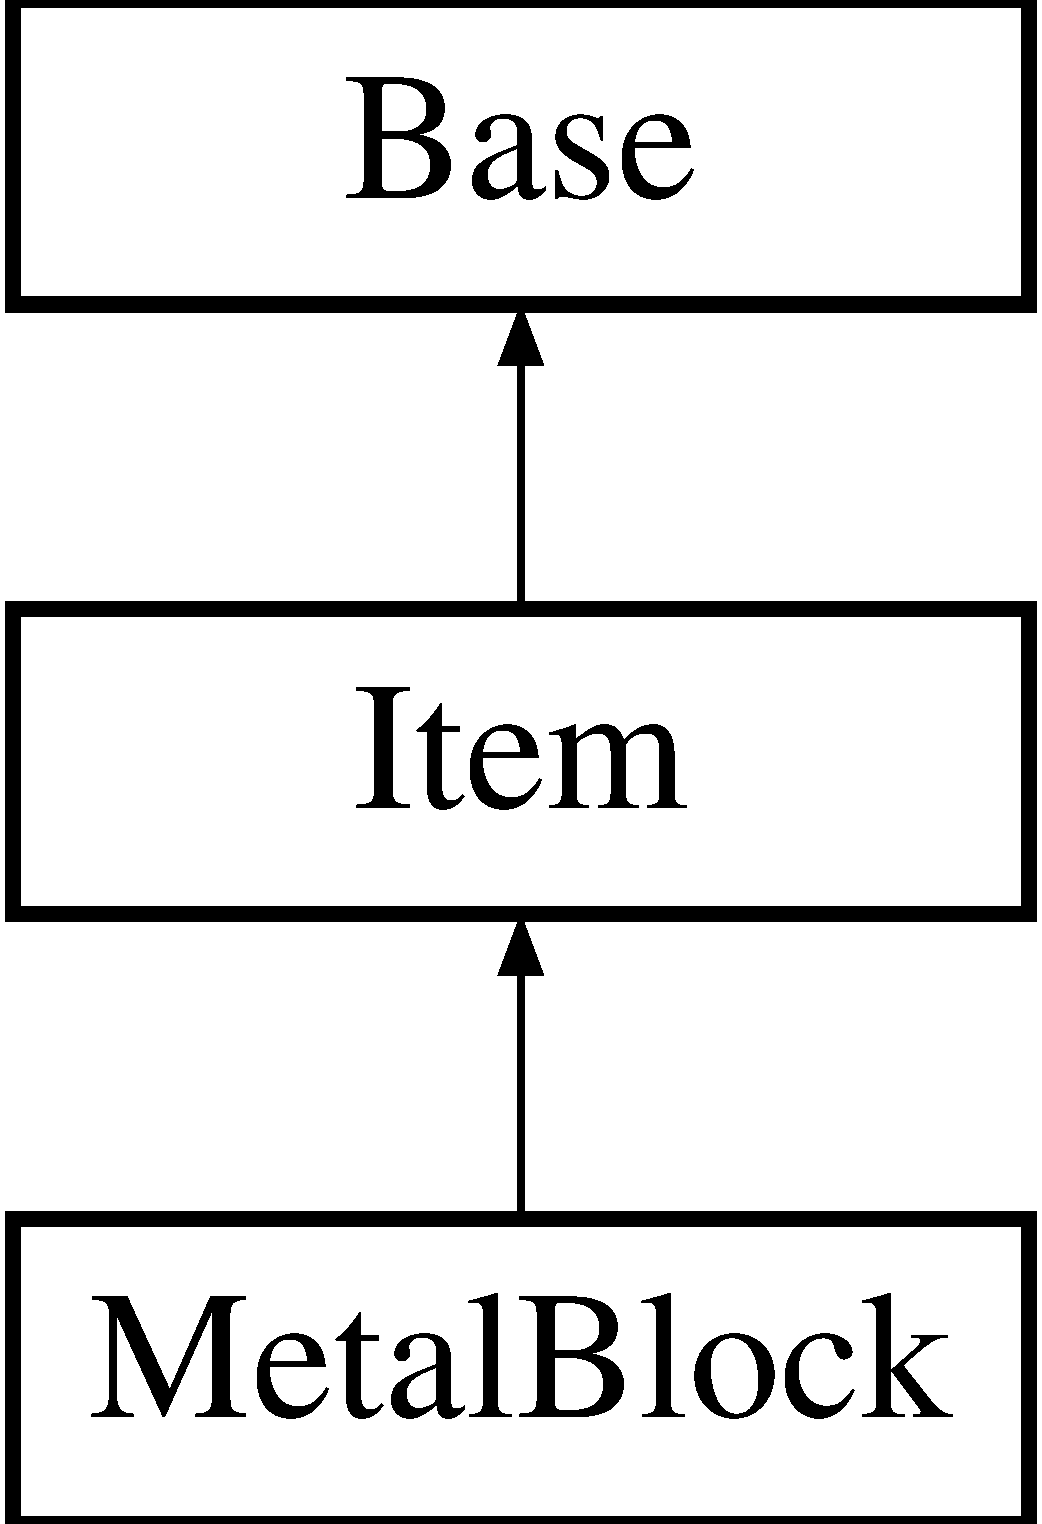
\includegraphics[height=3.000000cm]{classMetalBlock}
\end{center}
\end{figure}
\subsection*{Public Member Functions}
\begin{DoxyCompactItemize}
\item 
\hyperlink{classMetalBlock_a7798c893e774be284f76ed6093ac0144}{Metal\-Block} ()
\item 
void \hyperlink{classMetalBlock_a3eeed50e628c1b553fa145b0ff3aaa8a}{update} (\hyperlink{classShipMaster}{Ship\-Master} \&ship)
\item 
bool \hyperlink{classMetalBlock_ae5da009046d9443f292fbf7d955d3dc9}{interact} (\hyperlink{classPerson}{Person} \&person)
\item 
bool \hyperlink{classMetalBlock_a58537a96320a39f4c46659994698c394}{place} (\hyperlink{classPerson}{Person} \&person)
\item 
bool \hyperlink{classMetalBlock_a3ebb02bfb392a81c292d8f1fa0e7054e}{can\-Place} (\hyperlink{classPerson}{Person} \&person)
\item 
int \hyperlink{classMetalBlock_aed60769587273b97c098defb6bb19a0f}{get\-Texture\-I\-D} ()
\end{DoxyCompactItemize}
\subsection*{Additional Inherited Members}


\subsection{Constructor \& Destructor Documentation}
\hypertarget{classMetalBlock_a7798c893e774be284f76ed6093ac0144}{\index{Metal\-Block@{Metal\-Block}!Metal\-Block@{Metal\-Block}}
\index{Metal\-Block@{Metal\-Block}!MetalBlock@{Metal\-Block}}
\subsubsection[{Metal\-Block}]{\setlength{\rightskip}{0pt plus 5cm}Metal\-Block\-::\-Metal\-Block (
\begin{DoxyParamCaption}
{}
\end{DoxyParamCaption}
)}}\label{classMetalBlock_a7798c893e774be284f76ed6093ac0144}


\subsection{Member Function Documentation}
\hypertarget{classMetalBlock_a3ebb02bfb392a81c292d8f1fa0e7054e}{\index{Metal\-Block@{Metal\-Block}!can\-Place@{can\-Place}}
\index{can\-Place@{can\-Place}!MetalBlock@{Metal\-Block}}
\subsubsection[{can\-Place}]{\setlength{\rightskip}{0pt plus 5cm}bool Metal\-Block\-::can\-Place (
\begin{DoxyParamCaption}
\item[{{\bf Person} \&}]{person}
\end{DoxyParamCaption}
)\hspace{0.3cm}{\ttfamily [virtual]}}}\label{classMetalBlock_a3ebb02bfb392a81c292d8f1fa0e7054e}


Implements \hyperlink{classItem_afa9967b10984b1886ed6097eab7239e3}{Item}.

\hypertarget{classMetalBlock_aed60769587273b97c098defb6bb19a0f}{\index{Metal\-Block@{Metal\-Block}!get\-Texture\-I\-D@{get\-Texture\-I\-D}}
\index{get\-Texture\-I\-D@{get\-Texture\-I\-D}!MetalBlock@{Metal\-Block}}
\subsubsection[{get\-Texture\-I\-D}]{\setlength{\rightskip}{0pt plus 5cm}int Metal\-Block\-::get\-Texture\-I\-D (
\begin{DoxyParamCaption}
{}
\end{DoxyParamCaption}
)\hspace{0.3cm}{\ttfamily [virtual]}}}\label{classMetalBlock_aed60769587273b97c098defb6bb19a0f}


Implements \hyperlink{classItem_a38889163e99a1f5ec9b811b8e64fbc36}{Item}.

\hypertarget{classMetalBlock_ae5da009046d9443f292fbf7d955d3dc9}{\index{Metal\-Block@{Metal\-Block}!interact@{interact}}
\index{interact@{interact}!MetalBlock@{Metal\-Block}}
\subsubsection[{interact}]{\setlength{\rightskip}{0pt plus 5cm}bool Metal\-Block\-::interact (
\begin{DoxyParamCaption}
\item[{{\bf Person} \&}]{person}
\end{DoxyParamCaption}
)\hspace{0.3cm}{\ttfamily [virtual]}}}\label{classMetalBlock_ae5da009046d9443f292fbf7d955d3dc9}


Implements \hyperlink{classItem_a65a4d68109b4aa82c62d262ab4786145}{Item}.

\hypertarget{classMetalBlock_a58537a96320a39f4c46659994698c394}{\index{Metal\-Block@{Metal\-Block}!place@{place}}
\index{place@{place}!MetalBlock@{Metal\-Block}}
\subsubsection[{place}]{\setlength{\rightskip}{0pt plus 5cm}bool Metal\-Block\-::place (
\begin{DoxyParamCaption}
\item[{{\bf Person} \&}]{person}
\end{DoxyParamCaption}
)\hspace{0.3cm}{\ttfamily [virtual]}}}\label{classMetalBlock_a58537a96320a39f4c46659994698c394}


Implements \hyperlink{classItem_a2fc04b2fdd729977c419e0a1c5c8fa87}{Item}.

\hypertarget{classMetalBlock_a3eeed50e628c1b553fa145b0ff3aaa8a}{\index{Metal\-Block@{Metal\-Block}!update@{update}}
\index{update@{update}!MetalBlock@{Metal\-Block}}
\subsubsection[{update}]{\setlength{\rightskip}{0pt plus 5cm}void Metal\-Block\-::update (
\begin{DoxyParamCaption}
\item[{{\bf Ship\-Master} \&}]{ship}
\end{DoxyParamCaption}
)\hspace{0.3cm}{\ttfamily [virtual]}}}\label{classMetalBlock_a3eeed50e628c1b553fa145b0ff3aaa8a}


Implements \hyperlink{classItem_af7cb35b77955c00a38fc0f952da762f4}{Item}.



The documentation for this class was generated from the following files\-:\begin{DoxyCompactItemize}
\item 
core/items/\hyperlink{MetalBlock_8h}{Metal\-Block.\-h}\item 
core/items/\hyperlink{MetalBlock_8cpp}{Metal\-Block.\-cpp}\end{DoxyCompactItemize}

\hypertarget{classMetalWall}{\section{Metal\-Wall Class Reference}
\label{classMetalWall}\index{Metal\-Wall@{Metal\-Wall}}
}


{\ttfamily \#include $<$Metal\-Wall.\-h$>$}

Inheritance diagram for Metal\-Wall\-:\begin{figure}[H]
\begin{center}
\leavevmode
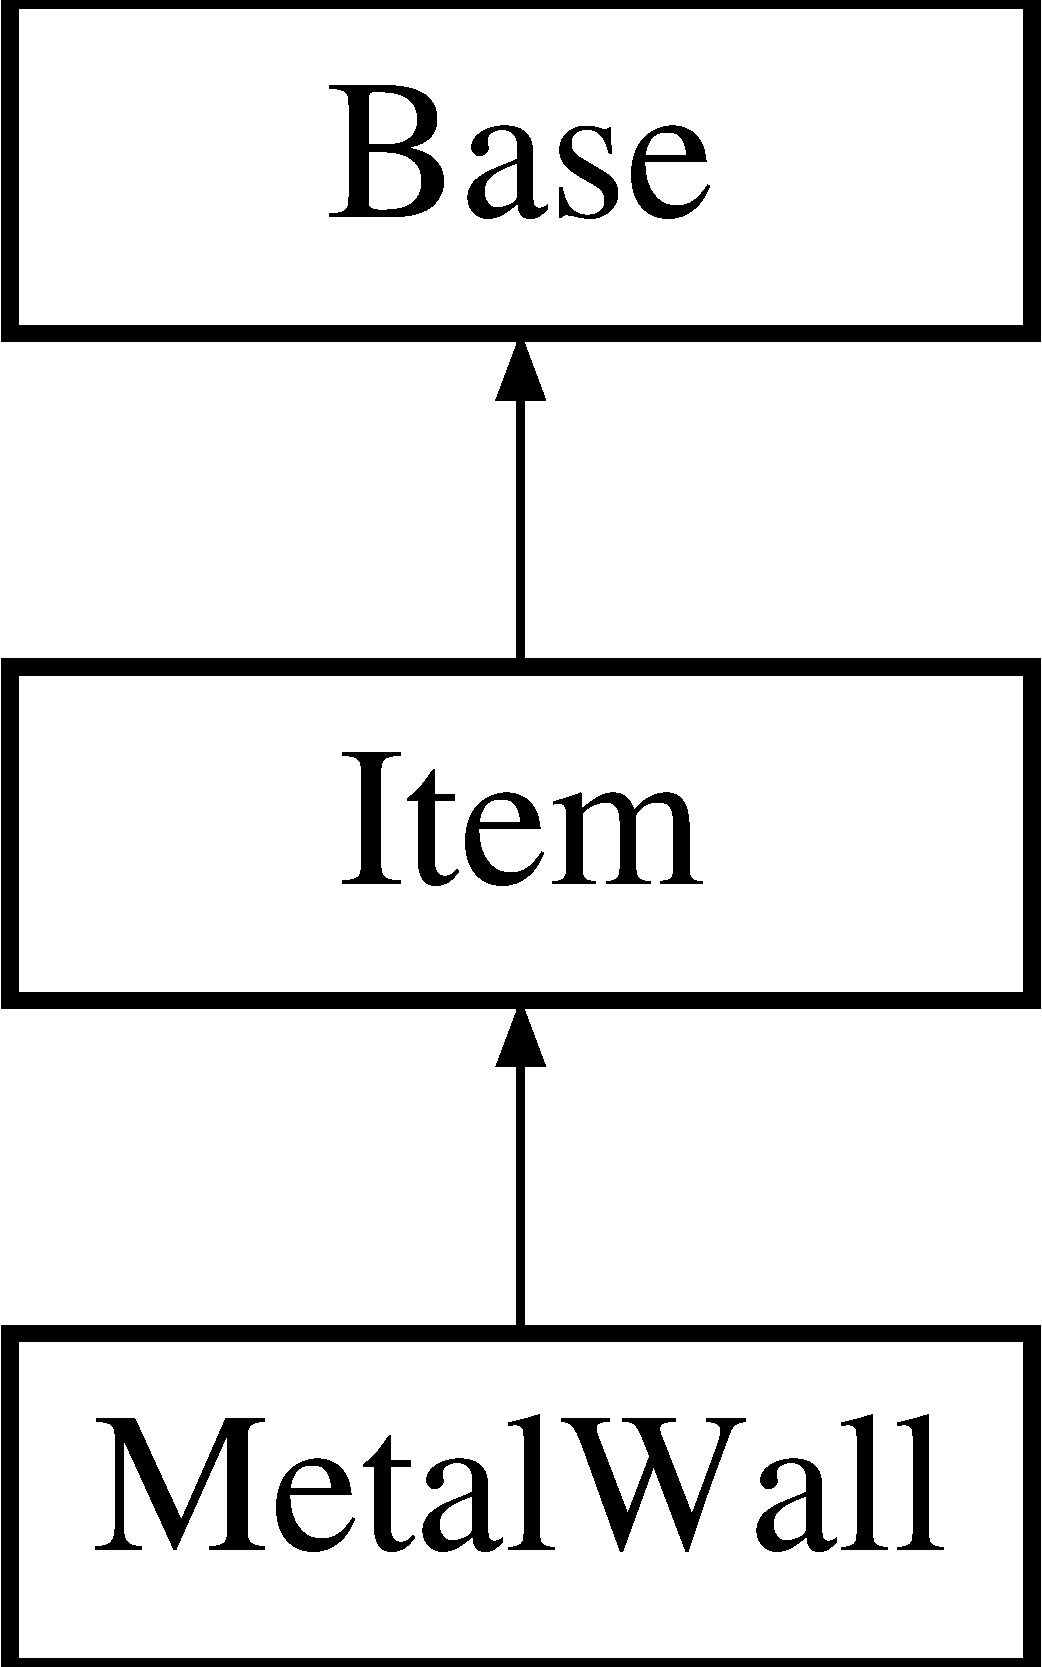
\includegraphics[height=3.000000cm]{classMetalWall}
\end{center}
\end{figure}
\subsection*{Public Member Functions}
\begin{DoxyCompactItemize}
\item 
\hyperlink{classMetalWall_af8274cdad365bb892c0f8c6eb23a86bd}{Metal\-Wall} ()
\item 
void \hyperlink{classMetalWall_a1beefd8e4e1e8a12d0f0c97a0286722e}{update} (\hyperlink{classShipMaster}{Ship\-Master} \&ship)
\item 
bool \hyperlink{classMetalWall_a6c5791ba1b0f1c4c6b9f064ceb0d217d}{interact} (\hyperlink{classPerson}{Person} \&person)
\item 
bool \hyperlink{classMetalWall_abd5c87f2cde822123cecaafb24edddd4}{place} (\hyperlink{classPerson}{Person} \&person)
\item 
bool \hyperlink{classMetalWall_acd888cb6afaa418a3a92f14eda27a9a5}{can\-Place} (\hyperlink{classPerson}{Person} \&person)
\item 
int \hyperlink{classMetalWall_a2c647de3c51c744da75cae0096e0042d}{get\-Texture\-I\-D} ()
\end{DoxyCompactItemize}
\subsection*{Additional Inherited Members}


\subsection{Constructor \& Destructor Documentation}
\hypertarget{classMetalWall_af8274cdad365bb892c0f8c6eb23a86bd}{\index{Metal\-Wall@{Metal\-Wall}!Metal\-Wall@{Metal\-Wall}}
\index{Metal\-Wall@{Metal\-Wall}!MetalWall@{Metal\-Wall}}
\subsubsection[{Metal\-Wall}]{\setlength{\rightskip}{0pt plus 5cm}Metal\-Wall\-::\-Metal\-Wall (
\begin{DoxyParamCaption}
{}
\end{DoxyParamCaption}
)}}\label{classMetalWall_af8274cdad365bb892c0f8c6eb23a86bd}


\subsection{Member Function Documentation}
\hypertarget{classMetalWall_acd888cb6afaa418a3a92f14eda27a9a5}{\index{Metal\-Wall@{Metal\-Wall}!can\-Place@{can\-Place}}
\index{can\-Place@{can\-Place}!MetalWall@{Metal\-Wall}}
\subsubsection[{can\-Place}]{\setlength{\rightskip}{0pt plus 5cm}bool Metal\-Wall\-::can\-Place (
\begin{DoxyParamCaption}
\item[{{\bf Person} \&}]{person}
\end{DoxyParamCaption}
)\hspace{0.3cm}{\ttfamily [virtual]}}}\label{classMetalWall_acd888cb6afaa418a3a92f14eda27a9a5}


Implements \hyperlink{classItem_afa9967b10984b1886ed6097eab7239e3}{Item}.

\hypertarget{classMetalWall_a2c647de3c51c744da75cae0096e0042d}{\index{Metal\-Wall@{Metal\-Wall}!get\-Texture\-I\-D@{get\-Texture\-I\-D}}
\index{get\-Texture\-I\-D@{get\-Texture\-I\-D}!MetalWall@{Metal\-Wall}}
\subsubsection[{get\-Texture\-I\-D}]{\setlength{\rightskip}{0pt plus 5cm}int Metal\-Wall\-::get\-Texture\-I\-D (
\begin{DoxyParamCaption}
{}
\end{DoxyParamCaption}
)\hspace{0.3cm}{\ttfamily [virtual]}}}\label{classMetalWall_a2c647de3c51c744da75cae0096e0042d}


Implements \hyperlink{classItem_a38889163e99a1f5ec9b811b8e64fbc36}{Item}.

\hypertarget{classMetalWall_a6c5791ba1b0f1c4c6b9f064ceb0d217d}{\index{Metal\-Wall@{Metal\-Wall}!interact@{interact}}
\index{interact@{interact}!MetalWall@{Metal\-Wall}}
\subsubsection[{interact}]{\setlength{\rightskip}{0pt plus 5cm}bool Metal\-Wall\-::interact (
\begin{DoxyParamCaption}
\item[{{\bf Person} \&}]{person}
\end{DoxyParamCaption}
)\hspace{0.3cm}{\ttfamily [virtual]}}}\label{classMetalWall_a6c5791ba1b0f1c4c6b9f064ceb0d217d}


Implements \hyperlink{classItem_a65a4d68109b4aa82c62d262ab4786145}{Item}.

\hypertarget{classMetalWall_abd5c87f2cde822123cecaafb24edddd4}{\index{Metal\-Wall@{Metal\-Wall}!place@{place}}
\index{place@{place}!MetalWall@{Metal\-Wall}}
\subsubsection[{place}]{\setlength{\rightskip}{0pt plus 5cm}bool Metal\-Wall\-::place (
\begin{DoxyParamCaption}
\item[{{\bf Person} \&}]{person}
\end{DoxyParamCaption}
)\hspace{0.3cm}{\ttfamily [virtual]}}}\label{classMetalWall_abd5c87f2cde822123cecaafb24edddd4}


Implements \hyperlink{classItem_a2fc04b2fdd729977c419e0a1c5c8fa87}{Item}.

\hypertarget{classMetalWall_a1beefd8e4e1e8a12d0f0c97a0286722e}{\index{Metal\-Wall@{Metal\-Wall}!update@{update}}
\index{update@{update}!MetalWall@{Metal\-Wall}}
\subsubsection[{update}]{\setlength{\rightskip}{0pt plus 5cm}void Metal\-Wall\-::update (
\begin{DoxyParamCaption}
\item[{{\bf Ship\-Master} \&}]{ship}
\end{DoxyParamCaption}
)\hspace{0.3cm}{\ttfamily [virtual]}}}\label{classMetalWall_a1beefd8e4e1e8a12d0f0c97a0286722e}


Implements \hyperlink{classItem_af7cb35b77955c00a38fc0f952da762f4}{Item}.



The documentation for this class was generated from the following files\-:\begin{DoxyCompactItemize}
\item 
core/items/\hyperlink{MetalWall_8h}{Metal\-Wall.\-h}\item 
core/items/\hyperlink{MetalWall_8cpp}{Metal\-Wall.\-cpp}\end{DoxyCompactItemize}

\hypertarget{classPath}{\section{Path Class Reference}
\label{classPath}\index{Path@{Path}}
}


Contains a path, usually from a pathfinding algorithm.  




{\ttfamily \#include $<$Path.\-h$>$}

\subsection*{Public Member Functions}
\begin{DoxyCompactItemize}
\item 
\hyperlink{classPath_af26cfab021ddf49af73da3b2beca85ac}{Path} ()
\item 
\hyperlink{classPath_ab3bdc2d36faec392cee7036599cac1e8}{Path} (unsigned int $\ast$\hyperlink{classPath_a15e858fcafd08883c9aa4460e9a63961}{path}, int \hyperlink{classPath_a899a5337cfcdac6fb6ff020dd7b4cf7d}{length})
\begin{DoxyCompactList}\small\item\em Constructor. \end{DoxyCompactList}\item 
\hyperlink{classPath_a141da9ff89c85e0ba410b5a73864c267}{$\sim$\-Path} ()
\item 
\hyperlink{classPath_a7e773507a877600083364271852ed19f}{Path} (const \hyperlink{classPath}{Path} \&obj)
\item 
\hyperlink{classPath}{Path} \& \hyperlink{classPath_a8fed62e1c09866defe99985648111462}{operator=} (const \hyperlink{classPath}{Path} \&obj)
\item 
void \hyperlink{classPath_ab9976c0fbf9ef118d8fb321aa904afbc}{copy} (const \hyperlink{classPath}{Path} \&obj)
\item 
unsigned int \hyperlink{classPath_a03ca062f08b780af43c39e27f02425c9}{get\-Next\-Direction} ()
\begin{DoxyCompactList}\small\item\em Get the next direction. \end{DoxyCompactList}\item 
bool \hyperlink{classPath_a025d58fe0a4ba7e2e525ac39f2e42d48}{is\-Complete} ()
\item 
bool \hyperlink{classPath_ab164e32a921ddff93de3206fbc9223ab}{has\-Path} ()
\item 
int \hyperlink{classPath_adf15aa16c75bdf6a02b9a52af0264a54}{get\-Length} ()
\end{DoxyCompactItemize}
\subsection*{Public Attributes}
\begin{DoxyCompactItemize}
\item 
unsigned int $\ast$ \hyperlink{classPath_a15e858fcafd08883c9aa4460e9a63961}{path}
\item 
int \hyperlink{classPath_a899a5337cfcdac6fb6ff020dd7b4cf7d}{length}
\item 
int \hyperlink{classPath_a2519662bb0102f3b02af7a739d55add7}{index}
\end{DoxyCompactItemize}


\subsection{Detailed Description}
Contains a path, usually from a pathfinding algorithm. 

\subsection{Constructor \& Destructor Documentation}
\hypertarget{classPath_af26cfab021ddf49af73da3b2beca85ac}{\index{Path@{Path}!Path@{Path}}
\index{Path@{Path}!Path@{Path}}
\subsubsection[{Path}]{\setlength{\rightskip}{0pt plus 5cm}Path\-::\-Path (
\begin{DoxyParamCaption}
{}
\end{DoxyParamCaption}
)}}\label{classPath_af26cfab021ddf49af73da3b2beca85ac}
\hypertarget{classPath_ab3bdc2d36faec392cee7036599cac1e8}{\index{Path@{Path}!Path@{Path}}
\index{Path@{Path}!Path@{Path}}
\subsubsection[{Path}]{\setlength{\rightskip}{0pt plus 5cm}Path\-::\-Path (
\begin{DoxyParamCaption}
\item[{unsigned int $\ast$}]{path, }
\item[{int}]{length}
\end{DoxyParamCaption}
)}}\label{classPath_ab3bdc2d36faec392cee7036599cac1e8}


Constructor. 

The length of path can be longer than length. 
\begin{DoxyParams}{Parameters}
{\em path} & Unsigned int array of directions. \\
\hline
{\em length} & Length of the array. \\
\hline
\end{DoxyParams}
\hypertarget{classPath_a141da9ff89c85e0ba410b5a73864c267}{\index{Path@{Path}!$\sim$\-Path@{$\sim$\-Path}}
\index{$\sim$\-Path@{$\sim$\-Path}!Path@{Path}}
\subsubsection[{$\sim$\-Path}]{\setlength{\rightskip}{0pt plus 5cm}Path\-::$\sim$\-Path (
\begin{DoxyParamCaption}
{}
\end{DoxyParamCaption}
)}}\label{classPath_a141da9ff89c85e0ba410b5a73864c267}
\hypertarget{classPath_a7e773507a877600083364271852ed19f}{\index{Path@{Path}!Path@{Path}}
\index{Path@{Path}!Path@{Path}}
\subsubsection[{Path}]{\setlength{\rightskip}{0pt plus 5cm}Path\-::\-Path (
\begin{DoxyParamCaption}
\item[{const {\bf Path} \&}]{obj}
\end{DoxyParamCaption}
)}}\label{classPath_a7e773507a877600083364271852ed19f}


\subsection{Member Function Documentation}
\hypertarget{classPath_ab9976c0fbf9ef118d8fb321aa904afbc}{\index{Path@{Path}!copy@{copy}}
\index{copy@{copy}!Path@{Path}}
\subsubsection[{copy}]{\setlength{\rightskip}{0pt plus 5cm}void Path\-::copy (
\begin{DoxyParamCaption}
\item[{const {\bf Path} \&}]{obj}
\end{DoxyParamCaption}
)}}\label{classPath_ab9976c0fbf9ef118d8fb321aa904afbc}
\hypertarget{classPath_adf15aa16c75bdf6a02b9a52af0264a54}{\index{Path@{Path}!get\-Length@{get\-Length}}
\index{get\-Length@{get\-Length}!Path@{Path}}
\subsubsection[{get\-Length}]{\setlength{\rightskip}{0pt plus 5cm}int Path\-::get\-Length (
\begin{DoxyParamCaption}
{}
\end{DoxyParamCaption}
)}}\label{classPath_adf15aa16c75bdf6a02b9a52af0264a54}
Get the length of the path. \hypertarget{classPath_a03ca062f08b780af43c39e27f02425c9}{\index{Path@{Path}!get\-Next\-Direction@{get\-Next\-Direction}}
\index{get\-Next\-Direction@{get\-Next\-Direction}!Path@{Path}}
\subsubsection[{get\-Next\-Direction}]{\setlength{\rightskip}{0pt plus 5cm}unsigned int Path\-::get\-Next\-Direction (
\begin{DoxyParamCaption}
{}
\end{DoxyParamCaption}
)}}\label{classPath_a03ca062f08b780af43c39e27f02425c9}


Get the next direction. 

\begin{DoxySeeAlso}{See Also}
\hyperlink{namespacedirections}{directions}. 
\end{DoxySeeAlso}
\hypertarget{classPath_ab164e32a921ddff93de3206fbc9223ab}{\index{Path@{Path}!has\-Path@{has\-Path}}
\index{has\-Path@{has\-Path}!Path@{Path}}
\subsubsection[{has\-Path}]{\setlength{\rightskip}{0pt plus 5cm}bool Path\-::has\-Path (
\begin{DoxyParamCaption}
{}
\end{DoxyParamCaption}
)}}\label{classPath_ab164e32a921ddff93de3206fbc9223ab}
Check if a path has been assigned to the object. \hypertarget{classPath_a025d58fe0a4ba7e2e525ac39f2e42d48}{\index{Path@{Path}!is\-Complete@{is\-Complete}}
\index{is\-Complete@{is\-Complete}!Path@{Path}}
\subsubsection[{is\-Complete}]{\setlength{\rightskip}{0pt plus 5cm}bool Path\-::is\-Complete (
\begin{DoxyParamCaption}
{}
\end{DoxyParamCaption}
)}}\label{classPath_a025d58fe0a4ba7e2e525ac39f2e42d48}
Check if the path has given it last direction. \hypertarget{classPath_a8fed62e1c09866defe99985648111462}{\index{Path@{Path}!operator=@{operator=}}
\index{operator=@{operator=}!Path@{Path}}
\subsubsection[{operator=}]{\setlength{\rightskip}{0pt plus 5cm}{\bf Path} \& Path\-::operator= (
\begin{DoxyParamCaption}
\item[{const {\bf Path} \&}]{obj}
\end{DoxyParamCaption}
)}}\label{classPath_a8fed62e1c09866defe99985648111462}


\subsection{Member Data Documentation}
\hypertarget{classPath_a2519662bb0102f3b02af7a739d55add7}{\index{Path@{Path}!index@{index}}
\index{index@{index}!Path@{Path}}
\subsubsection[{index}]{\setlength{\rightskip}{0pt plus 5cm}int Path\-::index}}\label{classPath_a2519662bb0102f3b02af7a739d55add7}
\hypertarget{classPath_a899a5337cfcdac6fb6ff020dd7b4cf7d}{\index{Path@{Path}!length@{length}}
\index{length@{length}!Path@{Path}}
\subsubsection[{length}]{\setlength{\rightskip}{0pt plus 5cm}int Path\-::length}}\label{classPath_a899a5337cfcdac6fb6ff020dd7b4cf7d}
\hypertarget{classPath_a15e858fcafd08883c9aa4460e9a63961}{\index{Path@{Path}!path@{path}}
\index{path@{path}!Path@{Path}}
\subsubsection[{path}]{\setlength{\rightskip}{0pt plus 5cm}unsigned int$\ast$ Path\-::path}}\label{classPath_a15e858fcafd08883c9aa4460e9a63961}


The documentation for this class was generated from the following files\-:\begin{DoxyCompactItemize}
\item 
core/map/\hyperlink{Path_8h}{Path.\-h}\item 
core/map/\hyperlink{Path_8cpp}{Path.\-cpp}\end{DoxyCompactItemize}

\hypertarget{classPathfinder}{\section{Pathfinder Class Reference}
\label{classPathfinder}\index{Pathfinder@{Pathfinder}}
}


Pathfinding algorithm object.  




{\ttfamily \#include $<$Pathfinder.\-h$>$}

\subsection*{Public Member Functions}
\begin{DoxyCompactItemize}
\item 
\hyperlink{classPathfinder_af562d840858cf2b369fcee51f5069456}{Pathfinder} ()
\begin{DoxyCompactList}\small\item\em Empty constructor. \end{DoxyCompactList}\item 
\hyperlink{classPathfinder_a52ace2447eb20a8736c9b6eecb2a39e4}{Pathfinder} (\hyperlink{classMatrix3D}{Matrix3\-D} \&map)
\begin{DoxyCompactList}\small\item\em Initialize the pathfinde with a local world map.  map Local world. \end{DoxyCompactList}\item 
\hyperlink{classPathfinder_a5b39561ad7375cfdc493d58cbb9fdc1b}{$\sim$\-Pathfinder} ()
\item 
\hyperlink{classPathfinder_ace22f0efc61b22a923f0c01fdcea0fb1}{Pathfinder} (const \hyperlink{classPathfinder}{Pathfinder} \&obj)
\item 
\hyperlink{classPathfinder}{Pathfinder} \& \hyperlink{classPathfinder_a7d1e82ebc1cf7c5f36a418f61721c61c}{operator=} (const \hyperlink{classPathfinder}{Pathfinder} \&obj)
\item 
void \hyperlink{classPathfinder_a2760969261a397539e0be0ec0ad25267}{copy} (const \hyperlink{classPathfinder}{Pathfinder} \&obj)
\begin{DoxyCompactList}\small\item\em Copy function. \end{DoxyCompactList}\item 
void \hyperlink{classPathfinder_aa92e55229fec296527e2975889fed2bd}{free\-Memory} ()
\begin{DoxyCompactList}\small\item\em Frees internal memory. \end{DoxyCompactList}\item 
void \hyperlink{classPathfinder_a20c13e5c6e005825b7536834867440b6}{free\-Path\-Nodes} ()
\begin{DoxyCompactList}\small\item\em Frees memory of node\-Hooks. \end{DoxyCompactList}\item 
void \hyperlink{classPathfinder_a3486c2d2a08f4b34ca76433dedda2642}{set\-Map} (\hyperlink{classMatrix3D}{Matrix3\-D} \&map)
\begin{DoxyCompactList}\small\item\em Assigned a different local world to the pathfinding object. \end{DoxyCompactList}\item 
\hyperlink{classPath}{Path} \hyperlink{classPathfinder_a211525380e7534f4721588e698b7a889}{find\-Path} (\hyperlink{structLocation}{Location} start, \hyperlink{structLocation}{Location} goal)
\begin{DoxyCompactList}\small\item\em Finds a path from start to goal. \end{DoxyCompactList}\end{DoxyCompactItemize}


\subsection{Detailed Description}
Pathfinding algorithm object. 

\begin{DoxySeeAlso}{See Also}
\hyperlink{classPathfinder_a211525380e7534f4721588e698b7a889}{find\-Path} 
\end{DoxySeeAlso}


\subsection{Constructor \& Destructor Documentation}
\hypertarget{classPathfinder_af562d840858cf2b369fcee51f5069456}{\index{Pathfinder@{Pathfinder}!Pathfinder@{Pathfinder}}
\index{Pathfinder@{Pathfinder}!Pathfinder@{Pathfinder}}
\subsubsection[{Pathfinder}]{\setlength{\rightskip}{0pt plus 5cm}Pathfinder\-::\-Pathfinder (
\begin{DoxyParamCaption}
{}
\end{DoxyParamCaption}
)}}\label{classPathfinder_af562d840858cf2b369fcee51f5069456}


Empty constructor. 

\hypertarget{classPathfinder_a52ace2447eb20a8736c9b6eecb2a39e4}{\index{Pathfinder@{Pathfinder}!Pathfinder@{Pathfinder}}
\index{Pathfinder@{Pathfinder}!Pathfinder@{Pathfinder}}
\subsubsection[{Pathfinder}]{\setlength{\rightskip}{0pt plus 5cm}Pathfinder\-::\-Pathfinder (
\begin{DoxyParamCaption}
\item[{{\bf Matrix3\-D} \&}]{map}
\end{DoxyParamCaption}
)}}\label{classPathfinder_a52ace2447eb20a8736c9b6eecb2a39e4}


Initialize the pathfinde with a local world map.  map Local world. 

\hypertarget{classPathfinder_a5b39561ad7375cfdc493d58cbb9fdc1b}{\index{Pathfinder@{Pathfinder}!$\sim$\-Pathfinder@{$\sim$\-Pathfinder}}
\index{$\sim$\-Pathfinder@{$\sim$\-Pathfinder}!Pathfinder@{Pathfinder}}
\subsubsection[{$\sim$\-Pathfinder}]{\setlength{\rightskip}{0pt plus 5cm}Pathfinder\-::$\sim$\-Pathfinder (
\begin{DoxyParamCaption}
{}
\end{DoxyParamCaption}
)}}\label{classPathfinder_a5b39561ad7375cfdc493d58cbb9fdc1b}
\hypertarget{classPathfinder_ace22f0efc61b22a923f0c01fdcea0fb1}{\index{Pathfinder@{Pathfinder}!Pathfinder@{Pathfinder}}
\index{Pathfinder@{Pathfinder}!Pathfinder@{Pathfinder}}
\subsubsection[{Pathfinder}]{\setlength{\rightskip}{0pt plus 5cm}Pathfinder\-::\-Pathfinder (
\begin{DoxyParamCaption}
\item[{const {\bf Pathfinder} \&}]{obj}
\end{DoxyParamCaption}
)}}\label{classPathfinder_ace22f0efc61b22a923f0c01fdcea0fb1}


\subsection{Member Function Documentation}
\hypertarget{classPathfinder_a2760969261a397539e0be0ec0ad25267}{\index{Pathfinder@{Pathfinder}!copy@{copy}}
\index{copy@{copy}!Pathfinder@{Pathfinder}}
\subsubsection[{copy}]{\setlength{\rightskip}{0pt plus 5cm}void Pathfinder\-::copy (
\begin{DoxyParamCaption}
\item[{const {\bf Pathfinder} \&}]{obj}
\end{DoxyParamCaption}
)}}\label{classPathfinder_a2760969261a397539e0be0ec0ad25267}


Copy function. 


\begin{DoxyParams}{Parameters}
{\em obj} & \hyperlink{classPathfinder}{Pathfinder} to copy. \\
\hline
\end{DoxyParams}
\hypertarget{classPathfinder_a211525380e7534f4721588e698b7a889}{\index{Pathfinder@{Pathfinder}!find\-Path@{find\-Path}}
\index{find\-Path@{find\-Path}!Pathfinder@{Pathfinder}}
\subsubsection[{find\-Path}]{\setlength{\rightskip}{0pt plus 5cm}{\bf Path} Pathfinder\-::find\-Path (
\begin{DoxyParamCaption}
\item[{{\bf Location}}]{start, }
\item[{{\bf Location}}]{goal}
\end{DoxyParamCaption}
)}}\label{classPathfinder_a211525380e7534f4721588e698b7a889}


Finds a path from start to goal. 


\begin{DoxyParams}{Parameters}
{\em start} & \hyperlink{structLocation}{Location} of start. \\
\hline
{\em goal} & \hyperlink{structLocation}{Location} of goal. \\
\hline
\end{DoxyParams}
\begin{DoxyReturn}{Returns}
A path object containg the path. 
\end{DoxyReturn}
\hypertarget{classPathfinder_aa92e55229fec296527e2975889fed2bd}{\index{Pathfinder@{Pathfinder}!free\-Memory@{free\-Memory}}
\index{free\-Memory@{free\-Memory}!Pathfinder@{Pathfinder}}
\subsubsection[{free\-Memory}]{\setlength{\rightskip}{0pt plus 5cm}void Pathfinder\-::free\-Memory (
\begin{DoxyParamCaption}
{}
\end{DoxyParamCaption}
)}}\label{classPathfinder_aa92e55229fec296527e2975889fed2bd}


Frees internal memory. 

\hypertarget{classPathfinder_a20c13e5c6e005825b7536834867440b6}{\index{Pathfinder@{Pathfinder}!free\-Path\-Nodes@{free\-Path\-Nodes}}
\index{free\-Path\-Nodes@{free\-Path\-Nodes}!Pathfinder@{Pathfinder}}
\subsubsection[{free\-Path\-Nodes}]{\setlength{\rightskip}{0pt plus 5cm}void Pathfinder\-::free\-Path\-Nodes (
\begin{DoxyParamCaption}
{}
\end{DoxyParamCaption}
)}}\label{classPathfinder_a20c13e5c6e005825b7536834867440b6}


Frees memory of node\-Hooks. 

\hypertarget{classPathfinder_a7d1e82ebc1cf7c5f36a418f61721c61c}{\index{Pathfinder@{Pathfinder}!operator=@{operator=}}
\index{operator=@{operator=}!Pathfinder@{Pathfinder}}
\subsubsection[{operator=}]{\setlength{\rightskip}{0pt plus 5cm}{\bf Pathfinder} \& Pathfinder\-::operator= (
\begin{DoxyParamCaption}
\item[{const {\bf Pathfinder} \&}]{obj}
\end{DoxyParamCaption}
)}}\label{classPathfinder_a7d1e82ebc1cf7c5f36a418f61721c61c}
\hypertarget{classPathfinder_a3486c2d2a08f4b34ca76433dedda2642}{\index{Pathfinder@{Pathfinder}!set\-Map@{set\-Map}}
\index{set\-Map@{set\-Map}!Pathfinder@{Pathfinder}}
\subsubsection[{set\-Map}]{\setlength{\rightskip}{0pt plus 5cm}void Pathfinder\-::set\-Map (
\begin{DoxyParamCaption}
\item[{{\bf Matrix3\-D} \&}]{map}
\end{DoxyParamCaption}
)}}\label{classPathfinder_a3486c2d2a08f4b34ca76433dedda2642}


Assigned a different local world to the pathfinding object. 


\begin{DoxyParams}{Parameters}
{\em map} & New local world. \\
\hline
\end{DoxyParams}


The documentation for this class was generated from the following files\-:\begin{DoxyCompactItemize}
\item 
core/map/\hyperlink{Pathfinder_8h}{Pathfinder.\-h}\item 
core/map/\hyperlink{Pathfinder_8cpp}{Pathfinder.\-cpp}\end{DoxyCompactItemize}

\hypertarget{structPathNode}{\section{Path\-Node Struct Reference}
\label{structPathNode}\index{Path\-Node@{Path\-Node}}
}


{\ttfamily \#include $<$Path\-Node.\-h$>$}

\subsection*{Public Member Functions}
\begin{DoxyCompactItemize}
\item 
\hyperlink{structPathNode_a8407a02423706e133bfea2b4c872289a}{Path\-Node} ()
\item 
\hyperlink{structPathNode_ab9bb9c07aad81a089e4cff8b2ba3f62b}{Path\-Node} (\hyperlink{structLocation}{Location} loc)
\item 
\hyperlink{structPathNode_a5cd5eedf94ada788f49d53350142f4f5}{Path\-Node} (int \hyperlink{structPathNode_a261418246914f0b5161419061859afb8}{x}, int \hyperlink{structPathNode_a1dba178e234b0a1e499e408985400107}{y}, int \hyperlink{structPathNode_ada356a6ae5e9463c3bf730a161639937}{z})
\item 
\hyperlink{structPathNode_a89625776708f7c5df719e07460c8ff4b}{Path\-Node} (const \hyperlink{structPathNode}{Path\-Node} \&obj)
\item 
\hyperlink{structPathNode}{Path\-Node} \& \hyperlink{structPathNode_a5b90811f20a6905e6e690ea43a441f3e}{operator=} (const \hyperlink{structPathNode}{Path\-Node} \&obj)
\item 
void \hyperlink{structPathNode_a2bd6a3ca0e38adeb9524d3b706b70b2b}{copy} (const \hyperlink{structPathNode}{Path\-Node} \&obj)
\end{DoxyCompactItemize}
\subsection*{Public Attributes}
\begin{DoxyCompactItemize}
\item 
int \hyperlink{structPathNode_a261418246914f0b5161419061859afb8}{x}
\item 
int \hyperlink{structPathNode_a1dba178e234b0a1e499e408985400107}{y}
\item 
int \hyperlink{structPathNode_ada356a6ae5e9463c3bf730a161639937}{z}
\item 
int \hyperlink{structPathNode_a6599b3700d0500aa34acf196649bce51}{f\-Value}
\item 
int \hyperlink{structPathNode_a90b21e2f0cf6142db81e7753f582b1cc}{g\-Value}
\end{DoxyCompactItemize}


\subsection{Constructor \& Destructor Documentation}
\hypertarget{structPathNode_a8407a02423706e133bfea2b4c872289a}{\index{Path\-Node@{Path\-Node}!Path\-Node@{Path\-Node}}
\index{Path\-Node@{Path\-Node}!PathNode@{Path\-Node}}
\subsubsection[{Path\-Node}]{\setlength{\rightskip}{0pt plus 5cm}Path\-Node\-::\-Path\-Node (
\begin{DoxyParamCaption}
{}
\end{DoxyParamCaption}
)\hspace{0.3cm}{\ttfamily [inline]}}}\label{structPathNode_a8407a02423706e133bfea2b4c872289a}
\hypertarget{structPathNode_ab9bb9c07aad81a089e4cff8b2ba3f62b}{\index{Path\-Node@{Path\-Node}!Path\-Node@{Path\-Node}}
\index{Path\-Node@{Path\-Node}!PathNode@{Path\-Node}}
\subsubsection[{Path\-Node}]{\setlength{\rightskip}{0pt plus 5cm}Path\-Node\-::\-Path\-Node (
\begin{DoxyParamCaption}
\item[{{\bf Location}}]{loc}
\end{DoxyParamCaption}
)\hspace{0.3cm}{\ttfamily [inline]}}}\label{structPathNode_ab9bb9c07aad81a089e4cff8b2ba3f62b}
\hypertarget{structPathNode_a5cd5eedf94ada788f49d53350142f4f5}{\index{Path\-Node@{Path\-Node}!Path\-Node@{Path\-Node}}
\index{Path\-Node@{Path\-Node}!PathNode@{Path\-Node}}
\subsubsection[{Path\-Node}]{\setlength{\rightskip}{0pt plus 5cm}Path\-Node\-::\-Path\-Node (
\begin{DoxyParamCaption}
\item[{int}]{x, }
\item[{int}]{y, }
\item[{int}]{z}
\end{DoxyParamCaption}
)\hspace{0.3cm}{\ttfamily [inline]}}}\label{structPathNode_a5cd5eedf94ada788f49d53350142f4f5}
\hypertarget{structPathNode_a89625776708f7c5df719e07460c8ff4b}{\index{Path\-Node@{Path\-Node}!Path\-Node@{Path\-Node}}
\index{Path\-Node@{Path\-Node}!PathNode@{Path\-Node}}
\subsubsection[{Path\-Node}]{\setlength{\rightskip}{0pt plus 5cm}Path\-Node\-::\-Path\-Node (
\begin{DoxyParamCaption}
\item[{const {\bf Path\-Node} \&}]{obj}
\end{DoxyParamCaption}
)\hspace{0.3cm}{\ttfamily [inline]}}}\label{structPathNode_a89625776708f7c5df719e07460c8ff4b}


\subsection{Member Function Documentation}
\hypertarget{structPathNode_a2bd6a3ca0e38adeb9524d3b706b70b2b}{\index{Path\-Node@{Path\-Node}!copy@{copy}}
\index{copy@{copy}!PathNode@{Path\-Node}}
\subsubsection[{copy}]{\setlength{\rightskip}{0pt plus 5cm}void Path\-Node\-::copy (
\begin{DoxyParamCaption}
\item[{const {\bf Path\-Node} \&}]{obj}
\end{DoxyParamCaption}
)\hspace{0.3cm}{\ttfamily [inline]}}}\label{structPathNode_a2bd6a3ca0e38adeb9524d3b706b70b2b}
\hypertarget{structPathNode_a5b90811f20a6905e6e690ea43a441f3e}{\index{Path\-Node@{Path\-Node}!operator=@{operator=}}
\index{operator=@{operator=}!PathNode@{Path\-Node}}
\subsubsection[{operator=}]{\setlength{\rightskip}{0pt plus 5cm}{\bf Path\-Node}\& Path\-Node\-::operator= (
\begin{DoxyParamCaption}
\item[{const {\bf Path\-Node} \&}]{obj}
\end{DoxyParamCaption}
)\hspace{0.3cm}{\ttfamily [inline]}}}\label{structPathNode_a5b90811f20a6905e6e690ea43a441f3e}


\subsection{Member Data Documentation}
\hypertarget{structPathNode_a6599b3700d0500aa34acf196649bce51}{\index{Path\-Node@{Path\-Node}!f\-Value@{f\-Value}}
\index{f\-Value@{f\-Value}!PathNode@{Path\-Node}}
\subsubsection[{f\-Value}]{\setlength{\rightskip}{0pt plus 5cm}int Path\-Node\-::f\-Value}}\label{structPathNode_a6599b3700d0500aa34acf196649bce51}
\hypertarget{structPathNode_a90b21e2f0cf6142db81e7753f582b1cc}{\index{Path\-Node@{Path\-Node}!g\-Value@{g\-Value}}
\index{g\-Value@{g\-Value}!PathNode@{Path\-Node}}
\subsubsection[{g\-Value}]{\setlength{\rightskip}{0pt plus 5cm}int Path\-Node\-::g\-Value}}\label{structPathNode_a90b21e2f0cf6142db81e7753f582b1cc}
\hypertarget{structPathNode_a261418246914f0b5161419061859afb8}{\index{Path\-Node@{Path\-Node}!x@{x}}
\index{x@{x}!PathNode@{Path\-Node}}
\subsubsection[{x}]{\setlength{\rightskip}{0pt plus 5cm}int Path\-Node\-::x}}\label{structPathNode_a261418246914f0b5161419061859afb8}
\hypertarget{structPathNode_a1dba178e234b0a1e499e408985400107}{\index{Path\-Node@{Path\-Node}!y@{y}}
\index{y@{y}!PathNode@{Path\-Node}}
\subsubsection[{y}]{\setlength{\rightskip}{0pt plus 5cm}int Path\-Node\-::y}}\label{structPathNode_a1dba178e234b0a1e499e408985400107}
\hypertarget{structPathNode_ada356a6ae5e9463c3bf730a161639937}{\index{Path\-Node@{Path\-Node}!z@{z}}
\index{z@{z}!PathNode@{Path\-Node}}
\subsubsection[{z}]{\setlength{\rightskip}{0pt plus 5cm}int Path\-Node\-::z}}\label{structPathNode_ada356a6ae5e9463c3bf730a161639937}


The documentation for this struct was generated from the following file\-:\begin{DoxyCompactItemize}
\item 
core/map/\hyperlink{PathNode_8h}{Path\-Node.\-h}\end{DoxyCompactItemize}

\hypertarget{classPerson}{\section{Person Class Reference}
\label{classPerson}\index{Person@{Person}}
}


{\ttfamily \#include $<$Person.\-h$>$}

Inheritance diagram for Person\-:\begin{figure}[H]
\begin{center}
\leavevmode
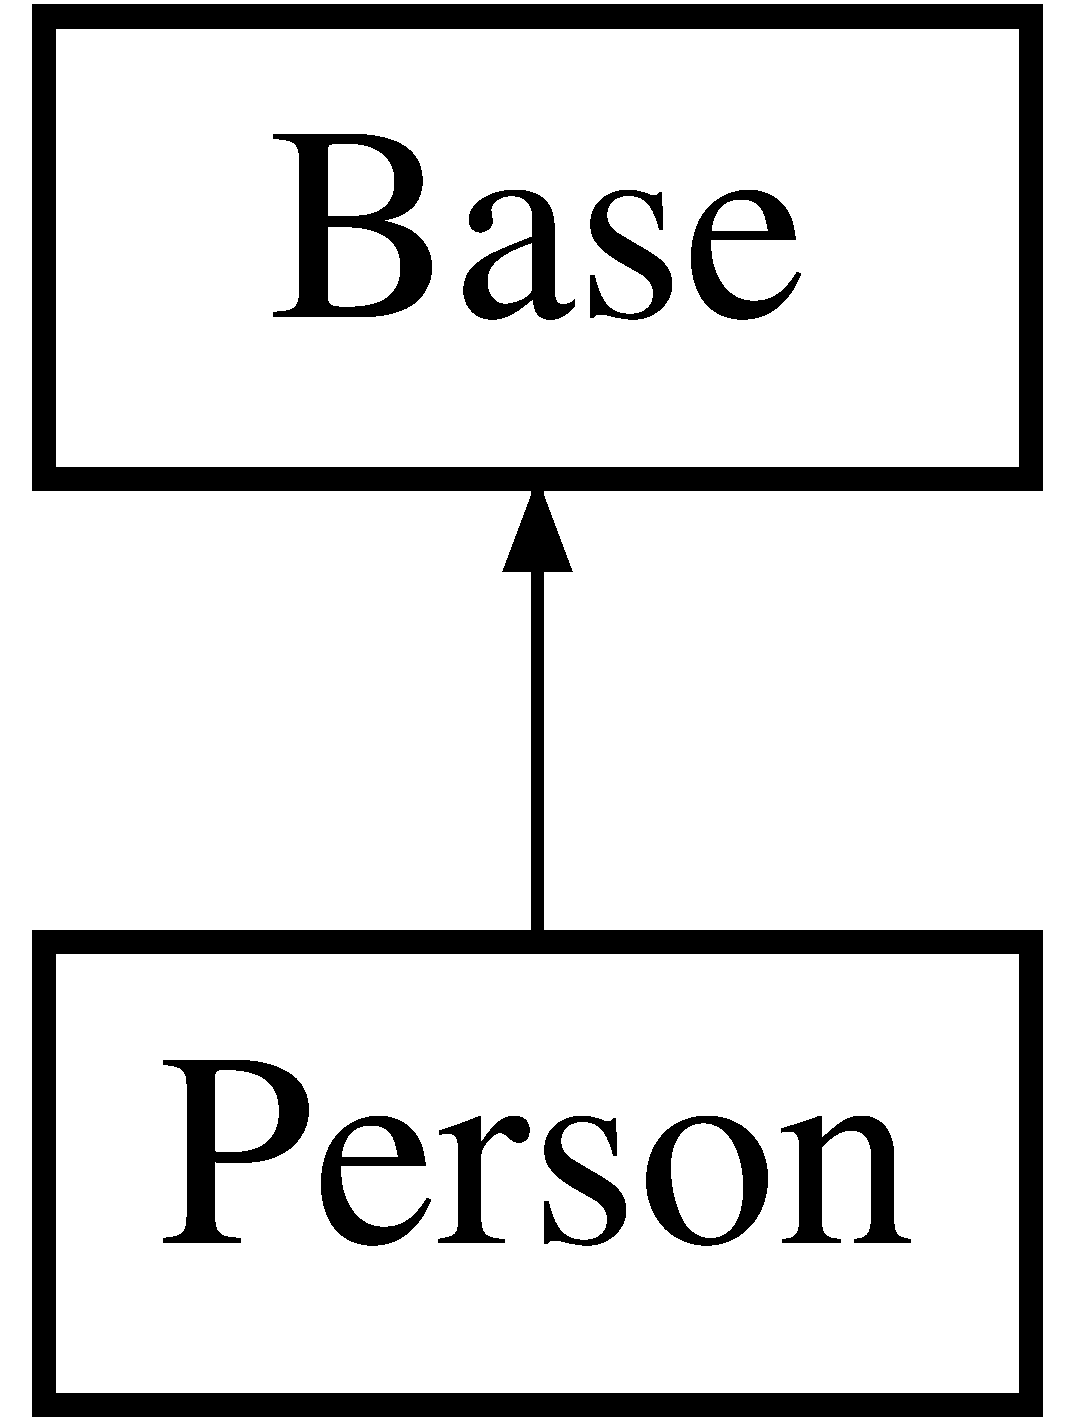
\includegraphics[height=2.000000cm]{classPerson}
\end{center}
\end{figure}
\subsection*{Public Member Functions}
\begin{DoxyCompactItemize}
\item 
\hyperlink{classPerson_a0397c6f89fafc12e738923f612bc41a3}{Person} ()
\item 
\hyperlink{classPerson_a700ffd693321c5fe6880262acf43d4da}{$\sim$\-Person} ()
\item 
void \hyperlink{classPerson_ae88c0a708c6a5c58fd76b305255c584e}{set\-Task} (\hyperlink{classTask}{Task} $\ast$\hyperlink{classPerson_a944dd7acfce7fb981e4c315f94b08ad9}{task})
\item 
bool \hyperlink{classPerson_a74924761363e651fbcde4aa0efb248f6}{has\-Task} ()
\item 
void \hyperlink{classPerson_ab895684028fe0d6a7bc23aec98ef8b0c}{update} ()
\item 
bool \hyperlink{classPerson_a0ce447d0c011c1060e9d5909f7621221}{add\-To\-Inventory} (int \hyperlink{classBase_a1dddc037afe2eae3e1364597e6a3cf46}{I\-D}, int amount)
\item 
bool \hyperlink{classPerson_ad266dba5486c59b07826bc2a78a2bc3e}{has\-In\-Inventory} (int \hyperlink{classBase_a1dddc037afe2eae3e1364597e6a3cf46}{I\-D}, int amount)
\item 
bool \hyperlink{classPerson_a7767ab0d8b5cdfc9cc69ce7739bf7be1}{take\-From\-Inventory} (int \hyperlink{classBase_a1dddc037afe2eae3e1364597e6a3cf46}{I\-D}, int amount)
\item 
int \hyperlink{classPerson_a9e7ac8aed6fa10fc1bba46e55779d7eb}{amount\-In\-Inventory} (int \hyperlink{classBase_a1dddc037afe2eae3e1364597e6a3cf46}{I\-D})
\end{DoxyCompactItemize}
\subsection*{Public Attributes}
\begin{DoxyCompactItemize}
\item 
\hyperlink{structLocation}{Location} \hyperlink{classPerson_a04c52986c5a7d61cb8a92e7069b22c11}{loc}
\item 
\hyperlink{classTask}{Task} $\ast$ \hyperlink{classPerson_a944dd7acfce7fb981e4c315f94b08ad9}{task}
\item 
unsigned int \hyperlink{classPerson_a26f2cf2da357f14c2185c218ca5c215c}{inventory} \mbox{[}\hyperlink{classPerson_a5d6040a07a5745a1dc62c6d6d540cca8}{I\-N\-V\-E\-N\-T\-O\-R\-Y\-\_\-\-S\-P\-A\-C\-E}\mbox{]}
\item 
unsigned int \hyperlink{classPerson_a98efc22a6f7c7f5fc099aa4fb7e70451}{inventory\-Amount} \mbox{[}\hyperlink{classPerson_a5d6040a07a5745a1dc62c6d6d540cca8}{I\-N\-V\-E\-N\-T\-O\-R\-Y\-\_\-\-S\-P\-A\-C\-E}\mbox{]}
\end{DoxyCompactItemize}
\subsection*{Static Public Attributes}
\begin{DoxyCompactItemize}
\item 
static const int \hyperlink{classPerson_a5d6040a07a5745a1dc62c6d6d540cca8}{I\-N\-V\-E\-N\-T\-O\-R\-Y\-\_\-\-S\-P\-A\-C\-E} = 5
\end{DoxyCompactItemize}


\subsection{Constructor \& Destructor Documentation}
\hypertarget{classPerson_a0397c6f89fafc12e738923f612bc41a3}{\index{Person@{Person}!Person@{Person}}
\index{Person@{Person}!Person@{Person}}
\subsubsection[{Person}]{\setlength{\rightskip}{0pt plus 5cm}Person\-::\-Person (
\begin{DoxyParamCaption}
{}
\end{DoxyParamCaption}
)}}\label{classPerson_a0397c6f89fafc12e738923f612bc41a3}
\hypertarget{classPerson_a700ffd693321c5fe6880262acf43d4da}{\index{Person@{Person}!$\sim$\-Person@{$\sim$\-Person}}
\index{$\sim$\-Person@{$\sim$\-Person}!Person@{Person}}
\subsubsection[{$\sim$\-Person}]{\setlength{\rightskip}{0pt plus 5cm}Person\-::$\sim$\-Person (
\begin{DoxyParamCaption}
{}
\end{DoxyParamCaption}
)}}\label{classPerson_a700ffd693321c5fe6880262acf43d4da}


\subsection{Member Function Documentation}
\hypertarget{classPerson_a0ce447d0c011c1060e9d5909f7621221}{\index{Person@{Person}!add\-To\-Inventory@{add\-To\-Inventory}}
\index{add\-To\-Inventory@{add\-To\-Inventory}!Person@{Person}}
\subsubsection[{add\-To\-Inventory}]{\setlength{\rightskip}{0pt plus 5cm}bool Person\-::add\-To\-Inventory (
\begin{DoxyParamCaption}
\item[{int}]{I\-D, }
\item[{int}]{amount}
\end{DoxyParamCaption}
)}}\label{classPerson_a0ce447d0c011c1060e9d5909f7621221}
\hypertarget{classPerson_a9e7ac8aed6fa10fc1bba46e55779d7eb}{\index{Person@{Person}!amount\-In\-Inventory@{amount\-In\-Inventory}}
\index{amount\-In\-Inventory@{amount\-In\-Inventory}!Person@{Person}}
\subsubsection[{amount\-In\-Inventory}]{\setlength{\rightskip}{0pt plus 5cm}int Person\-::amount\-In\-Inventory (
\begin{DoxyParamCaption}
\item[{int}]{I\-D}
\end{DoxyParamCaption}
)}}\label{classPerson_a9e7ac8aed6fa10fc1bba46e55779d7eb}
\hypertarget{classPerson_ad266dba5486c59b07826bc2a78a2bc3e}{\index{Person@{Person}!has\-In\-Inventory@{has\-In\-Inventory}}
\index{has\-In\-Inventory@{has\-In\-Inventory}!Person@{Person}}
\subsubsection[{has\-In\-Inventory}]{\setlength{\rightskip}{0pt plus 5cm}bool Person\-::has\-In\-Inventory (
\begin{DoxyParamCaption}
\item[{int}]{I\-D, }
\item[{int}]{amount}
\end{DoxyParamCaption}
)}}\label{classPerson_ad266dba5486c59b07826bc2a78a2bc3e}
\hypertarget{classPerson_a74924761363e651fbcde4aa0efb248f6}{\index{Person@{Person}!has\-Task@{has\-Task}}
\index{has\-Task@{has\-Task}!Person@{Person}}
\subsubsection[{has\-Task}]{\setlength{\rightskip}{0pt plus 5cm}bool Person\-::has\-Task (
\begin{DoxyParamCaption}
{}
\end{DoxyParamCaption}
)}}\label{classPerson_a74924761363e651fbcde4aa0efb248f6}
\hypertarget{classPerson_ae88c0a708c6a5c58fd76b305255c584e}{\index{Person@{Person}!set\-Task@{set\-Task}}
\index{set\-Task@{set\-Task}!Person@{Person}}
\subsubsection[{set\-Task}]{\setlength{\rightskip}{0pt plus 5cm}void Person\-::set\-Task (
\begin{DoxyParamCaption}
\item[{{\bf Task} $\ast$}]{task}
\end{DoxyParamCaption}
)}}\label{classPerson_ae88c0a708c6a5c58fd76b305255c584e}
\hypertarget{classPerson_a7767ab0d8b5cdfc9cc69ce7739bf7be1}{\index{Person@{Person}!take\-From\-Inventory@{take\-From\-Inventory}}
\index{take\-From\-Inventory@{take\-From\-Inventory}!Person@{Person}}
\subsubsection[{take\-From\-Inventory}]{\setlength{\rightskip}{0pt plus 5cm}bool Person\-::take\-From\-Inventory (
\begin{DoxyParamCaption}
\item[{int}]{I\-D, }
\item[{int}]{amount}
\end{DoxyParamCaption}
)}}\label{classPerson_a7767ab0d8b5cdfc9cc69ce7739bf7be1}
\hypertarget{classPerson_ab895684028fe0d6a7bc23aec98ef8b0c}{\index{Person@{Person}!update@{update}}
\index{update@{update}!Person@{Person}}
\subsubsection[{update}]{\setlength{\rightskip}{0pt plus 5cm}void Person\-::update (
\begin{DoxyParamCaption}
{}
\end{DoxyParamCaption}
)}}\label{classPerson_ab895684028fe0d6a7bc23aec98ef8b0c}


\subsection{Member Data Documentation}
\hypertarget{classPerson_a26f2cf2da357f14c2185c218ca5c215c}{\index{Person@{Person}!inventory@{inventory}}
\index{inventory@{inventory}!Person@{Person}}
\subsubsection[{inventory}]{\setlength{\rightskip}{0pt plus 5cm}unsigned int Person\-::inventory\mbox{[}{\bf I\-N\-V\-E\-N\-T\-O\-R\-Y\-\_\-\-S\-P\-A\-C\-E}\mbox{]}}}\label{classPerson_a26f2cf2da357f14c2185c218ca5c215c}
\hypertarget{classPerson_a5d6040a07a5745a1dc62c6d6d540cca8}{\index{Person@{Person}!I\-N\-V\-E\-N\-T\-O\-R\-Y\-\_\-\-S\-P\-A\-C\-E@{I\-N\-V\-E\-N\-T\-O\-R\-Y\-\_\-\-S\-P\-A\-C\-E}}
\index{I\-N\-V\-E\-N\-T\-O\-R\-Y\-\_\-\-S\-P\-A\-C\-E@{I\-N\-V\-E\-N\-T\-O\-R\-Y\-\_\-\-S\-P\-A\-C\-E}!Person@{Person}}
\subsubsection[{I\-N\-V\-E\-N\-T\-O\-R\-Y\-\_\-\-S\-P\-A\-C\-E}]{\setlength{\rightskip}{0pt plus 5cm}const int Person\-::\-I\-N\-V\-E\-N\-T\-O\-R\-Y\-\_\-\-S\-P\-A\-C\-E = 5\hspace{0.3cm}{\ttfamily [static]}}}\label{classPerson_a5d6040a07a5745a1dc62c6d6d540cca8}
\hypertarget{classPerson_a98efc22a6f7c7f5fc099aa4fb7e70451}{\index{Person@{Person}!inventory\-Amount@{inventory\-Amount}}
\index{inventory\-Amount@{inventory\-Amount}!Person@{Person}}
\subsubsection[{inventory\-Amount}]{\setlength{\rightskip}{0pt plus 5cm}unsigned int Person\-::inventory\-Amount\mbox{[}{\bf I\-N\-V\-E\-N\-T\-O\-R\-Y\-\_\-\-S\-P\-A\-C\-E}\mbox{]}}}\label{classPerson_a98efc22a6f7c7f5fc099aa4fb7e70451}
\hypertarget{classPerson_a04c52986c5a7d61cb8a92e7069b22c11}{\index{Person@{Person}!loc@{loc}}
\index{loc@{loc}!Person@{Person}}
\subsubsection[{loc}]{\setlength{\rightskip}{0pt plus 5cm}{\bf Location} Person\-::loc}}\label{classPerson_a04c52986c5a7d61cb8a92e7069b22c11}
\hypertarget{classPerson_a944dd7acfce7fb981e4c315f94b08ad9}{\index{Person@{Person}!task@{task}}
\index{task@{task}!Person@{Person}}
\subsubsection[{task}]{\setlength{\rightskip}{0pt plus 5cm}{\bf Task}$\ast$ Person\-::task}}\label{classPerson_a944dd7acfce7fb981e4c315f94b08ad9}


The documentation for this class was generated from the following files\-:\begin{DoxyCompactItemize}
\item 
core/enteties/\hyperlink{Person_8h}{Person.\-h}\item 
core/enteties/\hyperlink{Person_8cpp}{Person.\-cpp}\end{DoxyCompactItemize}

\hypertarget{structPriorityNode}{\section{Priority\-Node Struct Reference}
\label{structPriorityNode}\index{Priority\-Node@{Priority\-Node}}
}


{\ttfamily \#include $<$Priority\-Queue.\-h$>$}

\subsection*{Public Member Functions}
\begin{DoxyCompactItemize}
\item 
\hyperlink{structPriorityNode_aa2b185a2342809d7299cf8ba5e973363}{Priority\-Node} ()
\end{DoxyCompactItemize}
\subsection*{Public Attributes}
\begin{DoxyCompactItemize}
\item 
\hyperlink{structPriorityNode}{Priority\-Node} $\ast$ \hyperlink{structPriorityNode_a14b07ac4aa2d34e510f5183447698cc8}{link}
\item 
\hyperlink{structPathNode}{Path\-Node} $\ast$ \hyperlink{structPriorityNode_a4db59d39e0c8c22f7dc1bb15039dd717}{item}
\end{DoxyCompactItemize}


\subsection{Constructor \& Destructor Documentation}
\hypertarget{structPriorityNode_aa2b185a2342809d7299cf8ba5e973363}{\index{Priority\-Node@{Priority\-Node}!Priority\-Node@{Priority\-Node}}
\index{Priority\-Node@{Priority\-Node}!PriorityNode@{Priority\-Node}}
\subsubsection[{Priority\-Node}]{\setlength{\rightskip}{0pt plus 5cm}Priority\-Node\-::\-Priority\-Node (
\begin{DoxyParamCaption}
{}
\end{DoxyParamCaption}
)\hspace{0.3cm}{\ttfamily [inline]}}}\label{structPriorityNode_aa2b185a2342809d7299cf8ba5e973363}


\subsection{Member Data Documentation}
\hypertarget{structPriorityNode_a4db59d39e0c8c22f7dc1bb15039dd717}{\index{Priority\-Node@{Priority\-Node}!item@{item}}
\index{item@{item}!PriorityNode@{Priority\-Node}}
\subsubsection[{item}]{\setlength{\rightskip}{0pt plus 5cm}{\bf Path\-Node}$\ast$ Priority\-Node\-::item}}\label{structPriorityNode_a4db59d39e0c8c22f7dc1bb15039dd717}
\hypertarget{structPriorityNode_a14b07ac4aa2d34e510f5183447698cc8}{\index{Priority\-Node@{Priority\-Node}!link@{link}}
\index{link@{link}!PriorityNode@{Priority\-Node}}
\subsubsection[{link}]{\setlength{\rightskip}{0pt plus 5cm}{\bf Priority\-Node}$\ast$ Priority\-Node\-::link}}\label{structPriorityNode_a14b07ac4aa2d34e510f5183447698cc8}


The documentation for this struct was generated from the following file\-:\begin{DoxyCompactItemize}
\item 
core/map/\hyperlink{PriorityQueue_8h}{Priority\-Queue.\-h}\end{DoxyCompactItemize}

\hypertarget{classPriorityQueue}{\section{Priority\-Queue Class Reference}
\label{classPriorityQueue}\index{Priority\-Queue@{Priority\-Queue}}
}


{\ttfamily \#include $<$Priority\-Queue.\-h$>$}

\subsection*{Public Member Functions}
\begin{DoxyCompactItemize}
\item 
\hyperlink{classPriorityQueue_a43c56db471bb26fc2ae0f2ad90d81256}{Priority\-Queue} ()
\item 
\hyperlink{classPriorityQueue_a69b8f6b5ad108e9db66ac4db46c628d7}{$\sim$\-Priority\-Queue} ()
\item 
void \hyperlink{classPriorityQueue_ac4b66b5e38519272280b7c642b6e33cd}{push} (\hyperlink{structPathNode}{Path\-Node} $\ast$node)
\item 
\hyperlink{structPathNode}{Path\-Node} $\ast$ \hyperlink{classPriorityQueue_a6a32975106abaadce005966e21fa088d}{top} ()
\item 
bool \hyperlink{classPriorityQueue_ad3a482624abc3d4a87f74b1404ff201a}{has} (\hyperlink{structPathNode}{Path\-Node} $\ast$node)
\item 
void \hyperlink{classPriorityQueue_a9395579e928d279a1fc7c9302a130a29}{pop} ()
\item 
void \hyperlink{classPriorityQueue_a1d25b05db6d11496d3923fbf0d5d9acd}{clear} ()
\item 
bool \hyperlink{classPriorityQueue_a39f863f0a358df2a14a6388f3e347010}{empty} ()
\item 
int \hyperlink{classPriorityQueue_a9e739f490c722aa98a7d7560d46b8a51}{size} ()
\end{DoxyCompactItemize}


\subsection{Constructor \& Destructor Documentation}
\hypertarget{classPriorityQueue_a43c56db471bb26fc2ae0f2ad90d81256}{\index{Priority\-Queue@{Priority\-Queue}!Priority\-Queue@{Priority\-Queue}}
\index{Priority\-Queue@{Priority\-Queue}!PriorityQueue@{Priority\-Queue}}
\subsubsection[{Priority\-Queue}]{\setlength{\rightskip}{0pt plus 5cm}Priority\-Queue\-::\-Priority\-Queue (
\begin{DoxyParamCaption}
{}
\end{DoxyParamCaption}
)}}\label{classPriorityQueue_a43c56db471bb26fc2ae0f2ad90d81256}
\hypertarget{classPriorityQueue_a69b8f6b5ad108e9db66ac4db46c628d7}{\index{Priority\-Queue@{Priority\-Queue}!$\sim$\-Priority\-Queue@{$\sim$\-Priority\-Queue}}
\index{$\sim$\-Priority\-Queue@{$\sim$\-Priority\-Queue}!PriorityQueue@{Priority\-Queue}}
\subsubsection[{$\sim$\-Priority\-Queue}]{\setlength{\rightskip}{0pt plus 5cm}Priority\-Queue\-::$\sim$\-Priority\-Queue (
\begin{DoxyParamCaption}
{}
\end{DoxyParamCaption}
)}}\label{classPriorityQueue_a69b8f6b5ad108e9db66ac4db46c628d7}


\subsection{Member Function Documentation}
\hypertarget{classPriorityQueue_a1d25b05db6d11496d3923fbf0d5d9acd}{\index{Priority\-Queue@{Priority\-Queue}!clear@{clear}}
\index{clear@{clear}!PriorityQueue@{Priority\-Queue}}
\subsubsection[{clear}]{\setlength{\rightskip}{0pt plus 5cm}void Priority\-Queue\-::clear (
\begin{DoxyParamCaption}
{}
\end{DoxyParamCaption}
)}}\label{classPriorityQueue_a1d25b05db6d11496d3923fbf0d5d9acd}
\hypertarget{classPriorityQueue_a39f863f0a358df2a14a6388f3e347010}{\index{Priority\-Queue@{Priority\-Queue}!empty@{empty}}
\index{empty@{empty}!PriorityQueue@{Priority\-Queue}}
\subsubsection[{empty}]{\setlength{\rightskip}{0pt plus 5cm}bool Priority\-Queue\-::empty (
\begin{DoxyParamCaption}
{}
\end{DoxyParamCaption}
)}}\label{classPriorityQueue_a39f863f0a358df2a14a6388f3e347010}
\hypertarget{classPriorityQueue_ad3a482624abc3d4a87f74b1404ff201a}{\index{Priority\-Queue@{Priority\-Queue}!has@{has}}
\index{has@{has}!PriorityQueue@{Priority\-Queue}}
\subsubsection[{has}]{\setlength{\rightskip}{0pt plus 5cm}bool Priority\-Queue\-::has (
\begin{DoxyParamCaption}
\item[{{\bf Path\-Node} $\ast$}]{node}
\end{DoxyParamCaption}
)}}\label{classPriorityQueue_ad3a482624abc3d4a87f74b1404ff201a}
\hypertarget{classPriorityQueue_a9395579e928d279a1fc7c9302a130a29}{\index{Priority\-Queue@{Priority\-Queue}!pop@{pop}}
\index{pop@{pop}!PriorityQueue@{Priority\-Queue}}
\subsubsection[{pop}]{\setlength{\rightskip}{0pt plus 5cm}void Priority\-Queue\-::pop (
\begin{DoxyParamCaption}
{}
\end{DoxyParamCaption}
)}}\label{classPriorityQueue_a9395579e928d279a1fc7c9302a130a29}
\hypertarget{classPriorityQueue_ac4b66b5e38519272280b7c642b6e33cd}{\index{Priority\-Queue@{Priority\-Queue}!push@{push}}
\index{push@{push}!PriorityQueue@{Priority\-Queue}}
\subsubsection[{push}]{\setlength{\rightskip}{0pt plus 5cm}void Priority\-Queue\-::push (
\begin{DoxyParamCaption}
\item[{{\bf Path\-Node} $\ast$}]{node}
\end{DoxyParamCaption}
)}}\label{classPriorityQueue_ac4b66b5e38519272280b7c642b6e33cd}
\hypertarget{classPriorityQueue_a9e739f490c722aa98a7d7560d46b8a51}{\index{Priority\-Queue@{Priority\-Queue}!size@{size}}
\index{size@{size}!PriorityQueue@{Priority\-Queue}}
\subsubsection[{size}]{\setlength{\rightskip}{0pt plus 5cm}int Priority\-Queue\-::size (
\begin{DoxyParamCaption}
{}
\end{DoxyParamCaption}
)}}\label{classPriorityQueue_a9e739f490c722aa98a7d7560d46b8a51}
\hypertarget{classPriorityQueue_a6a32975106abaadce005966e21fa088d}{\index{Priority\-Queue@{Priority\-Queue}!top@{top}}
\index{top@{top}!PriorityQueue@{Priority\-Queue}}
\subsubsection[{top}]{\setlength{\rightskip}{0pt plus 5cm}{\bf Path\-Node} $\ast$ Priority\-Queue\-::top (
\begin{DoxyParamCaption}
{}
\end{DoxyParamCaption}
)}}\label{classPriorityQueue_a6a32975106abaadce005966e21fa088d}


The documentation for this class was generated from the following files\-:\begin{DoxyCompactItemize}
\item 
core/map/\hyperlink{PriorityQueue_8h}{Priority\-Queue.\-h}\item 
core/map/\hyperlink{PriorityQueue_8cpp}{Priority\-Queue.\-cpp}\end{DoxyCompactItemize}

\hypertarget{classRoom}{\section{Room Class Reference}
\label{classRoom}\index{Room@{Room}}
}


{\ttfamily \#include $<$Room.\-h$>$}

Inheritance diagram for Room\-:\begin{figure}[H]
\begin{center}
\leavevmode
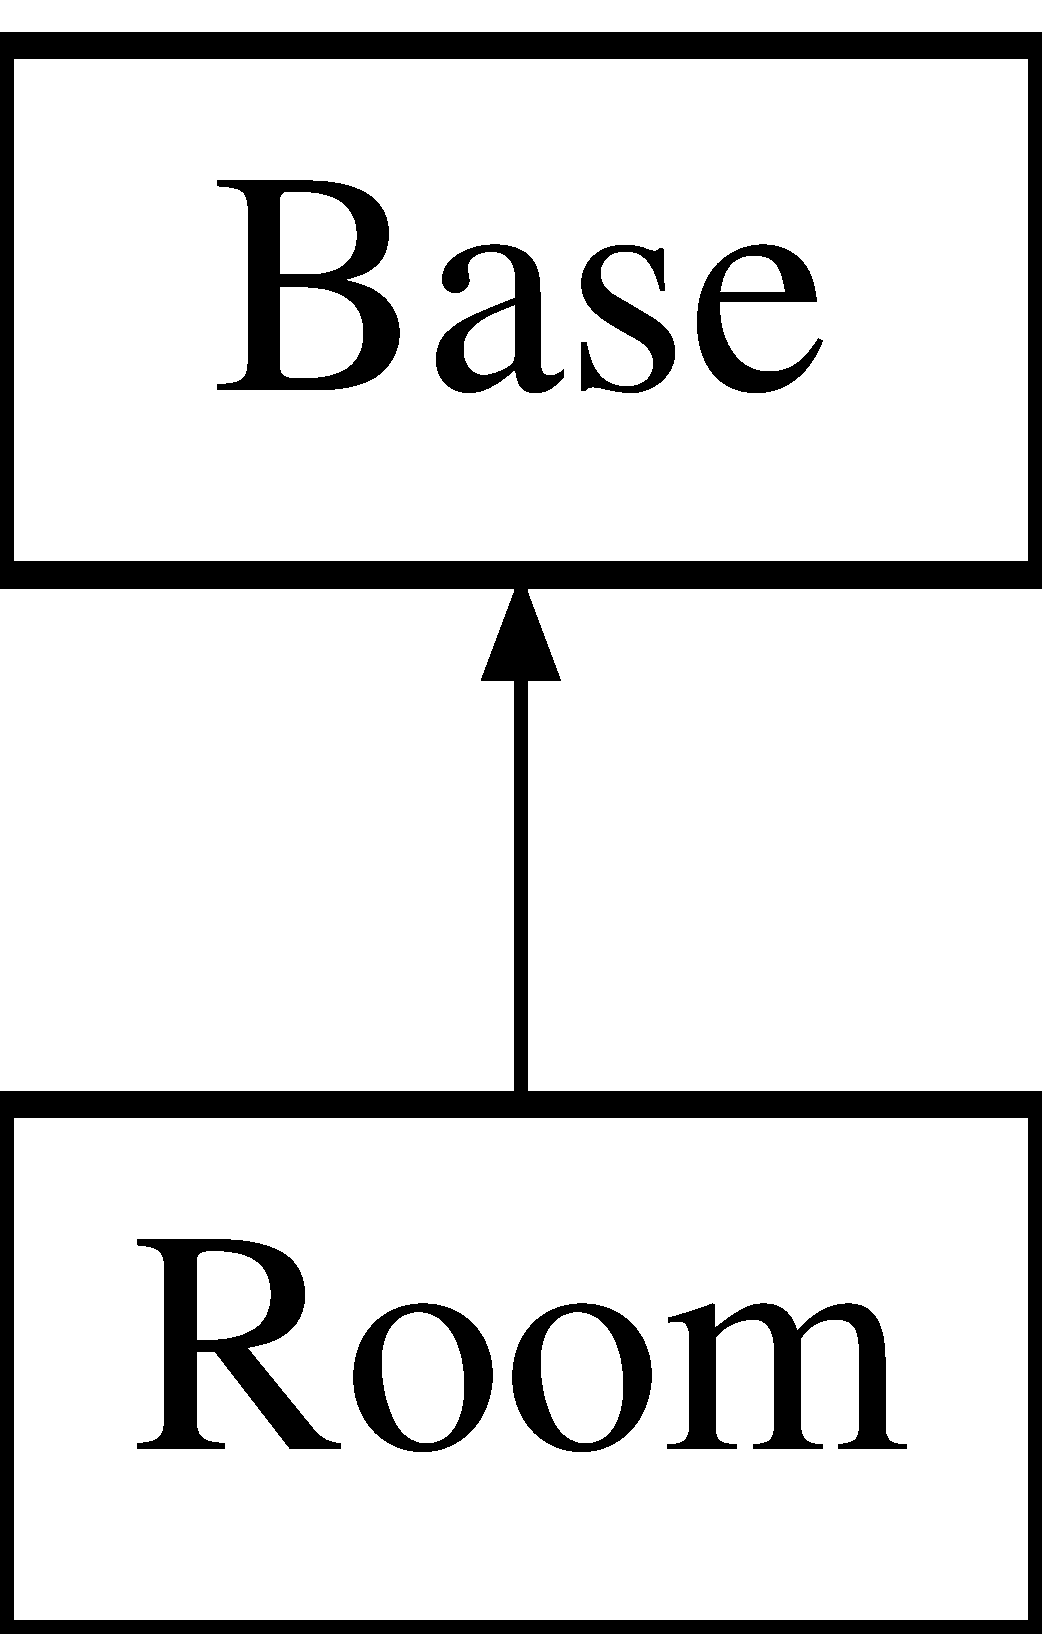
\includegraphics[height=2.000000cm]{classRoom}
\end{center}
\end{figure}
\subsection*{Public Member Functions}
\begin{DoxyCompactItemize}
\item 
\hyperlink{classRoom_ac6ef93a7d9c3e1d624e025058d5f16ff}{Room} ()
\item 
void \hyperlink{classRoom_af96fc605a002ba3d936a593bffed5d66}{add\-Item} (\hyperlink{classItem}{Item} $\ast$object)
\item 
\hyperlink{classItem}{Item} $\ast$ \hyperlink{classRoom_a3f3d6443a0050a9558bc9445012a2fc3}{get\-Item\-With\-U\-I\-D} (int \hyperlink{classBase_ac25c86b1d7bb8304fc0a81b8bddf7faf}{U\-I\-D}, bool remove)
\item 
int \hyperlink{classRoom_a1b59f0d10039c8f2683ecab81320887b}{get\-Item\-Cnt} ()
\item 
\hyperlink{classItem}{Item} $\ast$ \hyperlink{classRoom_a83a1e3f11cbe4ff4914bee88e920814e}{remove\-With\-U\-I\-D} (int \hyperlink{classBase_ac25c86b1d7bb8304fc0a81b8bddf7faf}{U\-I\-D})
\end{DoxyCompactItemize}
\subsection*{Public Attributes}
\begin{DoxyCompactItemize}
\item 
\hyperlink{structLocation}{Location} \hyperlink{classRoom_a160f390cd743ed1287815a41221a448b}{center}
\item 
\hyperlink{classLinkedList}{Linked\-List} \hyperlink{classRoom_a8e642143950831f3b9aa1faefff15b36}{objects}
\end{DoxyCompactItemize}


\subsection{Constructor \& Destructor Documentation}
\hypertarget{classRoom_ac6ef93a7d9c3e1d624e025058d5f16ff}{\index{Room@{Room}!Room@{Room}}
\index{Room@{Room}!Room@{Room}}
\subsubsection[{Room}]{\setlength{\rightskip}{0pt plus 5cm}Room\-::\-Room (
\begin{DoxyParamCaption}
{}
\end{DoxyParamCaption}
)}}\label{classRoom_ac6ef93a7d9c3e1d624e025058d5f16ff}


\subsection{Member Function Documentation}
\hypertarget{classRoom_af96fc605a002ba3d936a593bffed5d66}{\index{Room@{Room}!add\-Item@{add\-Item}}
\index{add\-Item@{add\-Item}!Room@{Room}}
\subsubsection[{add\-Item}]{\setlength{\rightskip}{0pt plus 5cm}void Room\-::add\-Item (
\begin{DoxyParamCaption}
\item[{{\bf Item} $\ast$}]{object}
\end{DoxyParamCaption}
)}}\label{classRoom_af96fc605a002ba3d936a593bffed5d66}
\hypertarget{classRoom_a1b59f0d10039c8f2683ecab81320887b}{\index{Room@{Room}!get\-Item\-Cnt@{get\-Item\-Cnt}}
\index{get\-Item\-Cnt@{get\-Item\-Cnt}!Room@{Room}}
\subsubsection[{get\-Item\-Cnt}]{\setlength{\rightskip}{0pt plus 5cm}int Room\-::get\-Item\-Cnt (
\begin{DoxyParamCaption}
{}
\end{DoxyParamCaption}
)}}\label{classRoom_a1b59f0d10039c8f2683ecab81320887b}
\hypertarget{classRoom_a3f3d6443a0050a9558bc9445012a2fc3}{\index{Room@{Room}!get\-Item\-With\-U\-I\-D@{get\-Item\-With\-U\-I\-D}}
\index{get\-Item\-With\-U\-I\-D@{get\-Item\-With\-U\-I\-D}!Room@{Room}}
\subsubsection[{get\-Item\-With\-U\-I\-D}]{\setlength{\rightskip}{0pt plus 5cm}{\bf Item} $\ast$ Room\-::get\-Item\-With\-U\-I\-D (
\begin{DoxyParamCaption}
\item[{int}]{U\-I\-D, }
\item[{bool}]{remove}
\end{DoxyParamCaption}
)}}\label{classRoom_a3f3d6443a0050a9558bc9445012a2fc3}
\hypertarget{classRoom_a83a1e3f11cbe4ff4914bee88e920814e}{\index{Room@{Room}!remove\-With\-U\-I\-D@{remove\-With\-U\-I\-D}}
\index{remove\-With\-U\-I\-D@{remove\-With\-U\-I\-D}!Room@{Room}}
\subsubsection[{remove\-With\-U\-I\-D}]{\setlength{\rightskip}{0pt plus 5cm}{\bf Item}$\ast$ Room\-::remove\-With\-U\-I\-D (
\begin{DoxyParamCaption}
\item[{int}]{U\-I\-D}
\end{DoxyParamCaption}
)}}\label{classRoom_a83a1e3f11cbe4ff4914bee88e920814e}


\subsection{Member Data Documentation}
\hypertarget{classRoom_a160f390cd743ed1287815a41221a448b}{\index{Room@{Room}!center@{center}}
\index{center@{center}!Room@{Room}}
\subsubsection[{center}]{\setlength{\rightskip}{0pt plus 5cm}{\bf Location} Room\-::center}}\label{classRoom_a160f390cd743ed1287815a41221a448b}
\hypertarget{classRoom_a8e642143950831f3b9aa1faefff15b36}{\index{Room@{Room}!objects@{objects}}
\index{objects@{objects}!Room@{Room}}
\subsubsection[{objects}]{\setlength{\rightskip}{0pt plus 5cm}{\bf Linked\-List} Room\-::objects}}\label{classRoom_a8e642143950831f3b9aa1faefff15b36}


The documentation for this class was generated from the following files\-:\begin{DoxyCompactItemize}
\item 
core/rooms/\hyperlink{Room_8h}{Room.\-h}\item 
core/rooms/\hyperlink{Room_8cpp}{Room.\-cpp}\end{DoxyCompactItemize}

\hypertarget{classShipCrew}{\section{Ship\-Crew Class Reference}
\label{classShipCrew}\index{Ship\-Crew@{Ship\-Crew}}
}


{\ttfamily \#include $<$Ship\-Crew.\-h$>$}

\subsection*{Public Member Functions}
\begin{DoxyCompactItemize}
\item 
\hyperlink{classShipCrew_a09256cf7b653e02e695947aa6a502021}{Ship\-Crew} ()
\item 
\hyperlink{classShipCrew_a8103bf86507ab0a53144cc130ea7017a}{$\sim$\-Ship\-Crew} ()
\item 
int \hyperlink{classShipCrew_adfcbfe662d0d9eafc7377c3e57848ca5}{get\-Crew\-Count} ()
\item 
\hyperlink{classPerson}{Person} $\ast$ \hyperlink{classShipCrew_a030e3995d99e3c8ca05595ecb6803ee9}{get\-Crew\-From\-Index} (int i)
\item 
\hyperlink{classPerson}{Person} $\ast$ \hyperlink{classShipCrew_a4eda642a62a32bf2e673e40adf3b4961}{create\-Crew\-Member} (int I\-D, \hyperlink{structLocation}{Location} loc)
\item 
\hyperlink{classPerson}{Person} $\ast$$\ast$ \hyperlink{classShipCrew_a70e2c2aacf48a0a673e167531f0c4f7e}{get\-Crew} ()
\item 
void \hyperlink{classShipCrew_ada9b840371438fccc3fa7b5023e1ff46}{update} (\hyperlink{classShipMaster}{Ship\-Master} \&ship)
\end{DoxyCompactItemize}
\subsection*{Public Attributes}
\begin{DoxyCompactItemize}
\item 
int \hyperlink{classShipCrew_acb418bcac20c237b52e992950480ced3}{cnt\-Crew}
\item 
\hyperlink{classPerson}{Person} $\ast$$\ast$ \hyperlink{classShipCrew_add436cb1633b1163196048997c525083}{crew}
\end{DoxyCompactItemize}


\subsection{Constructor \& Destructor Documentation}
\hypertarget{classShipCrew_a09256cf7b653e02e695947aa6a502021}{\index{Ship\-Crew@{Ship\-Crew}!Ship\-Crew@{Ship\-Crew}}
\index{Ship\-Crew@{Ship\-Crew}!ShipCrew@{Ship\-Crew}}
\subsubsection[{Ship\-Crew}]{\setlength{\rightskip}{0pt plus 5cm}Ship\-Crew\-::\-Ship\-Crew (
\begin{DoxyParamCaption}
{}
\end{DoxyParamCaption}
)}}\label{classShipCrew_a09256cf7b653e02e695947aa6a502021}
\hypertarget{classShipCrew_a8103bf86507ab0a53144cc130ea7017a}{\index{Ship\-Crew@{Ship\-Crew}!$\sim$\-Ship\-Crew@{$\sim$\-Ship\-Crew}}
\index{$\sim$\-Ship\-Crew@{$\sim$\-Ship\-Crew}!ShipCrew@{Ship\-Crew}}
\subsubsection[{$\sim$\-Ship\-Crew}]{\setlength{\rightskip}{0pt plus 5cm}Ship\-Crew\-::$\sim$\-Ship\-Crew (
\begin{DoxyParamCaption}
{}
\end{DoxyParamCaption}
)}}\label{classShipCrew_a8103bf86507ab0a53144cc130ea7017a}


\subsection{Member Function Documentation}
\hypertarget{classShipCrew_a4eda642a62a32bf2e673e40adf3b4961}{\index{Ship\-Crew@{Ship\-Crew}!create\-Crew\-Member@{create\-Crew\-Member}}
\index{create\-Crew\-Member@{create\-Crew\-Member}!ShipCrew@{Ship\-Crew}}
\subsubsection[{create\-Crew\-Member}]{\setlength{\rightskip}{0pt plus 5cm}{\bf Person} $\ast$ Ship\-Crew\-::create\-Crew\-Member (
\begin{DoxyParamCaption}
\item[{int}]{I\-D, }
\item[{{\bf Location}}]{loc}
\end{DoxyParamCaption}
)}}\label{classShipCrew_a4eda642a62a32bf2e673e40adf3b4961}
\hypertarget{classShipCrew_a70e2c2aacf48a0a673e167531f0c4f7e}{\index{Ship\-Crew@{Ship\-Crew}!get\-Crew@{get\-Crew}}
\index{get\-Crew@{get\-Crew}!ShipCrew@{Ship\-Crew}}
\subsubsection[{get\-Crew}]{\setlength{\rightskip}{0pt plus 5cm}{\bf Person} $\ast$$\ast$ Ship\-Crew\-::get\-Crew (
\begin{DoxyParamCaption}
{}
\end{DoxyParamCaption}
)}}\label{classShipCrew_a70e2c2aacf48a0a673e167531f0c4f7e}
\hypertarget{classShipCrew_adfcbfe662d0d9eafc7377c3e57848ca5}{\index{Ship\-Crew@{Ship\-Crew}!get\-Crew\-Count@{get\-Crew\-Count}}
\index{get\-Crew\-Count@{get\-Crew\-Count}!ShipCrew@{Ship\-Crew}}
\subsubsection[{get\-Crew\-Count}]{\setlength{\rightskip}{0pt plus 5cm}int Ship\-Crew\-::get\-Crew\-Count (
\begin{DoxyParamCaption}
{}
\end{DoxyParamCaption}
)}}\label{classShipCrew_adfcbfe662d0d9eafc7377c3e57848ca5}
\hypertarget{classShipCrew_a030e3995d99e3c8ca05595ecb6803ee9}{\index{Ship\-Crew@{Ship\-Crew}!get\-Crew\-From\-Index@{get\-Crew\-From\-Index}}
\index{get\-Crew\-From\-Index@{get\-Crew\-From\-Index}!ShipCrew@{Ship\-Crew}}
\subsubsection[{get\-Crew\-From\-Index}]{\setlength{\rightskip}{0pt plus 5cm}{\bf Person} $\ast$ Ship\-Crew\-::get\-Crew\-From\-Index (
\begin{DoxyParamCaption}
\item[{int}]{i}
\end{DoxyParamCaption}
)}}\label{classShipCrew_a030e3995d99e3c8ca05595ecb6803ee9}
\hypertarget{classShipCrew_ada9b840371438fccc3fa7b5023e1ff46}{\index{Ship\-Crew@{Ship\-Crew}!update@{update}}
\index{update@{update}!ShipCrew@{Ship\-Crew}}
\subsubsection[{update}]{\setlength{\rightskip}{0pt plus 5cm}void Ship\-Crew\-::update (
\begin{DoxyParamCaption}
\item[{{\bf Ship\-Master} \&}]{ship}
\end{DoxyParamCaption}
)}}\label{classShipCrew_ada9b840371438fccc3fa7b5023e1ff46}


\subsection{Member Data Documentation}
\hypertarget{classShipCrew_acb418bcac20c237b52e992950480ced3}{\index{Ship\-Crew@{Ship\-Crew}!cnt\-Crew@{cnt\-Crew}}
\index{cnt\-Crew@{cnt\-Crew}!ShipCrew@{Ship\-Crew}}
\subsubsection[{cnt\-Crew}]{\setlength{\rightskip}{0pt plus 5cm}int Ship\-Crew\-::cnt\-Crew}}\label{classShipCrew_acb418bcac20c237b52e992950480ced3}
\hypertarget{classShipCrew_add436cb1633b1163196048997c525083}{\index{Ship\-Crew@{Ship\-Crew}!crew@{crew}}
\index{crew@{crew}!ShipCrew@{Ship\-Crew}}
\subsubsection[{crew}]{\setlength{\rightskip}{0pt plus 5cm}{\bf Person}$\ast$$\ast$ Ship\-Crew\-::crew}}\label{classShipCrew_add436cb1633b1163196048997c525083}


The documentation for this class was generated from the following files\-:\begin{DoxyCompactItemize}
\item 
core/main/\hyperlink{ShipCrew_8h}{Ship\-Crew.\-h}\item 
core/main/\hyperlink{ShipCrew_8cpp}{Ship\-Crew.\-cpp}\end{DoxyCompactItemize}

\hypertarget{classShipItems}{\section{Ship\-Items Class Reference}
\label{classShipItems}\index{Ship\-Items@{Ship\-Items}}
}


{\ttfamily \#include $<$Ship\-Items.\-h$>$}

\subsection*{Public Member Functions}
\begin{DoxyCompactItemize}
\item 
\hyperlink{classShipItems_adc14b59e747ba46333bdd33b864392c6}{Ship\-Items} ()
\item 
\hyperlink{classShipItems_ae0d1231017d6e1c4b586a8c0bc398af7}{Ship\-Items} (int O, int N, int M)
\item 
\hyperlink{classShipItems_a41194d8cb17bfaa10a5cd6abb80ba78b}{$\sim$\-Ship\-Items} ()
\item 
void \hyperlink{classShipItems_a3a5ab7ad8035ae1b3b6da0483f5ce792}{update} (\hyperlink{classShipMaster}{Ship\-Master} \&ship)
\item 
\hyperlink{classItem}{Item} $\ast$ \hyperlink{classShipItems_a49cdd4419f853d178c0cc1afd105121a}{create\-Item} (int I\-D, int U\-I\-D, \hyperlink{structLocation}{Location} loc)
\item 
\hyperlink{classItem}{Item} $\ast$ \hyperlink{classShipItems_a61bdf01e758998d328b172e241aa816a}{create\-Item} (int I\-D, int U\-I\-D, \hyperlink{structLocation}{Location} loc, unsigned int direction)
\item 
bool \hyperlink{classShipItems_a838f560346a9d7b0f1bb128aaf93b1c7}{place\-Item} (\hyperlink{classItem}{Item} $\ast$obj)
\begin{DoxyCompactList}\small\item\em Place an item on the map, usually \char`\"{}activates\char`\"{} the item. \end{DoxyCompactList}\item 
\hyperlink{classLinkedList}{Linked\-List} \& \hyperlink{classShipItems_adf57cc0e0699cb38bdb29e8d45b1243d}{get\-Items} ()
\item 
\hyperlink{classLinkedList}{Linked\-List} \& \hyperlink{classShipItems_ac77750d78a0d268e330940a73961238f}{get\-Items\-Pending} ()
\item 
\hyperlink{classLinkedList}{Linked\-List} \& \hyperlink{classShipItems_a00f9e60d91680092094a012aa9bc7fc6}{get\-Items\-Weaponry} ()
\item 
\hyperlink{classLinkedList}{Linked\-List} \& \hyperlink{classShipItems_ae6e53eb02579b4e64ad640ba56fe3759}{get\-Texture\-List} ()
\item 
\hyperlink{classItem}{Item} $\ast$ \hyperlink{classShipItems_aaebf0d993affd21ec619233e0e654ae7}{get\-Item\-Placed\-From\-I\-D} (int I\-D)
\item 
\hyperlink{classItem}{Item} $\ast$ \hyperlink{classShipItems_a7204e19a3782177c271deddcd437af77}{get\-Item\-Placed\-From\-U\-I\-D} (int U\-I\-D)
\item 
\hyperlink{classItem}{Item} $\ast$ \hyperlink{classShipItems_a1e716d983b99a8e8c7ca730c9159e1ab}{get\-Item\-Placed\-From\-Index} (int i)
\item 
\hyperlink{classItem}{Item} $\ast$ \hyperlink{classShipItems_aa79604b85e2271567b30926eecedeb53}{get\-Item\-Pending\-From\-I\-D} (int I\-D)
\item 
\hyperlink{classItem}{Item} $\ast$ \hyperlink{classShipItems_aa30ae0f1bb8b3fc8201906fd031e78ec}{get\-Item\-Pending\-From\-U\-I\-D} (int U\-I\-D)
\item 
\hyperlink{classItem}{Item} $\ast$ \hyperlink{classShipItems_abb26bb09017b5f331f990833e959924b}{get\-Item\-Pending\-From\-Index} (int i)
\item 
int \hyperlink{classShipItems_ad48bad514797b873e253cf21a7d40288}{get\-Item\-Placed\-Count} ()
\item 
int \hyperlink{classShipItems_a9473269de6b8e8f7bdd41236ea294c1b}{get\-Item\-Pending\-Count} ()
\end{DoxyCompactItemize}
\subsection*{Public Attributes}
\begin{DoxyCompactItemize}
\item 
\hyperlink{classItemMatrix}{Item\-Matrix} \hyperlink{classShipItems_a465b928e53ec914789735aee07a7a719}{items\-Map\-Container}
\item 
\hyperlink{classLinkedList}{Linked\-List} \hyperlink{classShipItems_a3e71d1f18d3eee132394a9c524cb43e4}{items\-Placed}
\item 
\hyperlink{classLinkedList}{Linked\-List} \hyperlink{classShipItems_a4549ab087c77cf3bfade68ddec7ef8ee}{items\-Pending}
\item 
\hyperlink{classLinkedList}{Linked\-List} \hyperlink{classShipItems_afaec48b1818b5083c7d471ddce4430b3}{items\-Weaponry}
\item 
\hyperlink{classLinkedList}{Linked\-List} \hyperlink{classShipItems_adb0d04e59dc21442a04199a6d0043011}{texture\-List}
\item 
\hyperlink{classLinkedList}{Linked\-List} \hyperlink{classShipItems_ab9b7f9dcb3f50c2d724e150d5fa54cb4}{list\-Update}
\item 
\hyperlink{classLinkedList}{Linked\-List} $\ast$$\ast$$\ast$ \hyperlink{classShipItems_aaaa5d8305486800e29cdbf40861cda65}{items\-Map}
\end{DoxyCompactItemize}


\subsection{Constructor \& Destructor Documentation}
\hypertarget{classShipItems_adc14b59e747ba46333bdd33b864392c6}{\index{Ship\-Items@{Ship\-Items}!Ship\-Items@{Ship\-Items}}
\index{Ship\-Items@{Ship\-Items}!ShipItems@{Ship\-Items}}
\subsubsection[{Ship\-Items}]{\setlength{\rightskip}{0pt plus 5cm}Ship\-Items\-::\-Ship\-Items (
\begin{DoxyParamCaption}
{}
\end{DoxyParamCaption}
)}}\label{classShipItems_adc14b59e747ba46333bdd33b864392c6}
\hypertarget{classShipItems_ae0d1231017d6e1c4b586a8c0bc398af7}{\index{Ship\-Items@{Ship\-Items}!Ship\-Items@{Ship\-Items}}
\index{Ship\-Items@{Ship\-Items}!ShipItems@{Ship\-Items}}
\subsubsection[{Ship\-Items}]{\setlength{\rightskip}{0pt plus 5cm}Ship\-Items\-::\-Ship\-Items (
\begin{DoxyParamCaption}
\item[{int}]{O, }
\item[{int}]{N, }
\item[{int}]{M}
\end{DoxyParamCaption}
)}}\label{classShipItems_ae0d1231017d6e1c4b586a8c0bc398af7}
\hypertarget{classShipItems_a41194d8cb17bfaa10a5cd6abb80ba78b}{\index{Ship\-Items@{Ship\-Items}!$\sim$\-Ship\-Items@{$\sim$\-Ship\-Items}}
\index{$\sim$\-Ship\-Items@{$\sim$\-Ship\-Items}!ShipItems@{Ship\-Items}}
\subsubsection[{$\sim$\-Ship\-Items}]{\setlength{\rightskip}{0pt plus 5cm}Ship\-Items\-::$\sim$\-Ship\-Items (
\begin{DoxyParamCaption}
{}
\end{DoxyParamCaption}
)}}\label{classShipItems_a41194d8cb17bfaa10a5cd6abb80ba78b}


\subsection{Member Function Documentation}
\hypertarget{classShipItems_a49cdd4419f853d178c0cc1afd105121a}{\index{Ship\-Items@{Ship\-Items}!create\-Item@{create\-Item}}
\index{create\-Item@{create\-Item}!ShipItems@{Ship\-Items}}
\subsubsection[{create\-Item}]{\setlength{\rightskip}{0pt plus 5cm}{\bf Item} $\ast$ Ship\-Items\-::create\-Item (
\begin{DoxyParamCaption}
\item[{int}]{I\-D, }
\item[{int}]{U\-I\-D, }
\item[{{\bf Location}}]{loc}
\end{DoxyParamCaption}
)}}\label{classShipItems_a49cdd4419f853d178c0cc1afd105121a}
\hypertarget{classShipItems_a61bdf01e758998d328b172e241aa816a}{\index{Ship\-Items@{Ship\-Items}!create\-Item@{create\-Item}}
\index{create\-Item@{create\-Item}!ShipItems@{Ship\-Items}}
\subsubsection[{create\-Item}]{\setlength{\rightskip}{0pt plus 5cm}{\bf Item} $\ast$ Ship\-Items\-::create\-Item (
\begin{DoxyParamCaption}
\item[{int}]{I\-D, }
\item[{int}]{U\-I\-D, }
\item[{{\bf Location}}]{loc, }
\item[{unsigned int}]{direction}
\end{DoxyParamCaption}
)}}\label{classShipItems_a61bdf01e758998d328b172e241aa816a}
\hypertarget{classShipItems_a9473269de6b8e8f7bdd41236ea294c1b}{\index{Ship\-Items@{Ship\-Items}!get\-Item\-Pending\-Count@{get\-Item\-Pending\-Count}}
\index{get\-Item\-Pending\-Count@{get\-Item\-Pending\-Count}!ShipItems@{Ship\-Items}}
\subsubsection[{get\-Item\-Pending\-Count}]{\setlength{\rightskip}{0pt plus 5cm}int Ship\-Items\-::get\-Item\-Pending\-Count (
\begin{DoxyParamCaption}
{}
\end{DoxyParamCaption}
)}}\label{classShipItems_a9473269de6b8e8f7bdd41236ea294c1b}
\hypertarget{classShipItems_aa79604b85e2271567b30926eecedeb53}{\index{Ship\-Items@{Ship\-Items}!get\-Item\-Pending\-From\-I\-D@{get\-Item\-Pending\-From\-I\-D}}
\index{get\-Item\-Pending\-From\-I\-D@{get\-Item\-Pending\-From\-I\-D}!ShipItems@{Ship\-Items}}
\subsubsection[{get\-Item\-Pending\-From\-I\-D}]{\setlength{\rightskip}{0pt plus 5cm}{\bf Item} $\ast$ Ship\-Items\-::get\-Item\-Pending\-From\-I\-D (
\begin{DoxyParamCaption}
\item[{int}]{I\-D}
\end{DoxyParamCaption}
)}}\label{classShipItems_aa79604b85e2271567b30926eecedeb53}
\hypertarget{classShipItems_abb26bb09017b5f331f990833e959924b}{\index{Ship\-Items@{Ship\-Items}!get\-Item\-Pending\-From\-Index@{get\-Item\-Pending\-From\-Index}}
\index{get\-Item\-Pending\-From\-Index@{get\-Item\-Pending\-From\-Index}!ShipItems@{Ship\-Items}}
\subsubsection[{get\-Item\-Pending\-From\-Index}]{\setlength{\rightskip}{0pt plus 5cm}{\bf Item}$\ast$ Ship\-Items\-::get\-Item\-Pending\-From\-Index (
\begin{DoxyParamCaption}
\item[{int}]{i}
\end{DoxyParamCaption}
)}}\label{classShipItems_abb26bb09017b5f331f990833e959924b}
\hypertarget{classShipItems_aa30ae0f1bb8b3fc8201906fd031e78ec}{\index{Ship\-Items@{Ship\-Items}!get\-Item\-Pending\-From\-U\-I\-D@{get\-Item\-Pending\-From\-U\-I\-D}}
\index{get\-Item\-Pending\-From\-U\-I\-D@{get\-Item\-Pending\-From\-U\-I\-D}!ShipItems@{Ship\-Items}}
\subsubsection[{get\-Item\-Pending\-From\-U\-I\-D}]{\setlength{\rightskip}{0pt plus 5cm}{\bf Item} $\ast$ Ship\-Items\-::get\-Item\-Pending\-From\-U\-I\-D (
\begin{DoxyParamCaption}
\item[{int}]{U\-I\-D}
\end{DoxyParamCaption}
)}}\label{classShipItems_aa30ae0f1bb8b3fc8201906fd031e78ec}
\hypertarget{classShipItems_ad48bad514797b873e253cf21a7d40288}{\index{Ship\-Items@{Ship\-Items}!get\-Item\-Placed\-Count@{get\-Item\-Placed\-Count}}
\index{get\-Item\-Placed\-Count@{get\-Item\-Placed\-Count}!ShipItems@{Ship\-Items}}
\subsubsection[{get\-Item\-Placed\-Count}]{\setlength{\rightskip}{0pt plus 5cm}int Ship\-Items\-::get\-Item\-Placed\-Count (
\begin{DoxyParamCaption}
{}
\end{DoxyParamCaption}
)}}\label{classShipItems_ad48bad514797b873e253cf21a7d40288}
\hypertarget{classShipItems_aaebf0d993affd21ec619233e0e654ae7}{\index{Ship\-Items@{Ship\-Items}!get\-Item\-Placed\-From\-I\-D@{get\-Item\-Placed\-From\-I\-D}}
\index{get\-Item\-Placed\-From\-I\-D@{get\-Item\-Placed\-From\-I\-D}!ShipItems@{Ship\-Items}}
\subsubsection[{get\-Item\-Placed\-From\-I\-D}]{\setlength{\rightskip}{0pt plus 5cm}{\bf Item} $\ast$ Ship\-Items\-::get\-Item\-Placed\-From\-I\-D (
\begin{DoxyParamCaption}
\item[{int}]{I\-D}
\end{DoxyParamCaption}
)}}\label{classShipItems_aaebf0d993affd21ec619233e0e654ae7}
\hypertarget{classShipItems_a1e716d983b99a8e8c7ca730c9159e1ab}{\index{Ship\-Items@{Ship\-Items}!get\-Item\-Placed\-From\-Index@{get\-Item\-Placed\-From\-Index}}
\index{get\-Item\-Placed\-From\-Index@{get\-Item\-Placed\-From\-Index}!ShipItems@{Ship\-Items}}
\subsubsection[{get\-Item\-Placed\-From\-Index}]{\setlength{\rightskip}{0pt plus 5cm}{\bf Item}$\ast$ Ship\-Items\-::get\-Item\-Placed\-From\-Index (
\begin{DoxyParamCaption}
\item[{int}]{i}
\end{DoxyParamCaption}
)}}\label{classShipItems_a1e716d983b99a8e8c7ca730c9159e1ab}
\hypertarget{classShipItems_a7204e19a3782177c271deddcd437af77}{\index{Ship\-Items@{Ship\-Items}!get\-Item\-Placed\-From\-U\-I\-D@{get\-Item\-Placed\-From\-U\-I\-D}}
\index{get\-Item\-Placed\-From\-U\-I\-D@{get\-Item\-Placed\-From\-U\-I\-D}!ShipItems@{Ship\-Items}}
\subsubsection[{get\-Item\-Placed\-From\-U\-I\-D}]{\setlength{\rightskip}{0pt plus 5cm}{\bf Item} $\ast$ Ship\-Items\-::get\-Item\-Placed\-From\-U\-I\-D (
\begin{DoxyParamCaption}
\item[{int}]{U\-I\-D}
\end{DoxyParamCaption}
)}}\label{classShipItems_a7204e19a3782177c271deddcd437af77}
\hypertarget{classShipItems_adf57cc0e0699cb38bdb29e8d45b1243d}{\index{Ship\-Items@{Ship\-Items}!get\-Items@{get\-Items}}
\index{get\-Items@{get\-Items}!ShipItems@{Ship\-Items}}
\subsubsection[{get\-Items}]{\setlength{\rightskip}{0pt plus 5cm}{\bf Linked\-List} \& Ship\-Items\-::get\-Items (
\begin{DoxyParamCaption}
{}
\end{DoxyParamCaption}
)}}\label{classShipItems_adf57cc0e0699cb38bdb29e8d45b1243d}
\hypertarget{classShipItems_ac77750d78a0d268e330940a73961238f}{\index{Ship\-Items@{Ship\-Items}!get\-Items\-Pending@{get\-Items\-Pending}}
\index{get\-Items\-Pending@{get\-Items\-Pending}!ShipItems@{Ship\-Items}}
\subsubsection[{get\-Items\-Pending}]{\setlength{\rightskip}{0pt plus 5cm}{\bf Linked\-List} \& Ship\-Items\-::get\-Items\-Pending (
\begin{DoxyParamCaption}
{}
\end{DoxyParamCaption}
)}}\label{classShipItems_ac77750d78a0d268e330940a73961238f}
\hypertarget{classShipItems_a00f9e60d91680092094a012aa9bc7fc6}{\index{Ship\-Items@{Ship\-Items}!get\-Items\-Weaponry@{get\-Items\-Weaponry}}
\index{get\-Items\-Weaponry@{get\-Items\-Weaponry}!ShipItems@{Ship\-Items}}
\subsubsection[{get\-Items\-Weaponry}]{\setlength{\rightskip}{0pt plus 5cm}{\bf Linked\-List}\& Ship\-Items\-::get\-Items\-Weaponry (
\begin{DoxyParamCaption}
{}
\end{DoxyParamCaption}
)}}\label{classShipItems_a00f9e60d91680092094a012aa9bc7fc6}
\hypertarget{classShipItems_ae6e53eb02579b4e64ad640ba56fe3759}{\index{Ship\-Items@{Ship\-Items}!get\-Texture\-List@{get\-Texture\-List}}
\index{get\-Texture\-List@{get\-Texture\-List}!ShipItems@{Ship\-Items}}
\subsubsection[{get\-Texture\-List}]{\setlength{\rightskip}{0pt plus 5cm}{\bf Linked\-List} \& Ship\-Items\-::get\-Texture\-List (
\begin{DoxyParamCaption}
{}
\end{DoxyParamCaption}
)}}\label{classShipItems_ae6e53eb02579b4e64ad640ba56fe3759}
\hypertarget{classShipItems_a838f560346a9d7b0f1bb128aaf93b1c7}{\index{Ship\-Items@{Ship\-Items}!place\-Item@{place\-Item}}
\index{place\-Item@{place\-Item}!ShipItems@{Ship\-Items}}
\subsubsection[{place\-Item}]{\setlength{\rightskip}{0pt plus 5cm}bool Ship\-Items\-::place\-Item (
\begin{DoxyParamCaption}
\item[{{\bf Item} $\ast$}]{obj}
\end{DoxyParamCaption}
)}}\label{classShipItems_a838f560346a9d7b0f1bb128aaf93b1c7}


Place an item on the map, usually \char`\"{}activates\char`\"{} the item. 

Used when an object has finished construction and is thus ready to be interacted with. This places the item in the corresponding lists it needs to placed in and will be used to block movement, get the placed variable set to true, and other things connected to being placed. \hypertarget{classShipItems_a3a5ab7ad8035ae1b3b6da0483f5ce792}{\index{Ship\-Items@{Ship\-Items}!update@{update}}
\index{update@{update}!ShipItems@{Ship\-Items}}
\subsubsection[{update}]{\setlength{\rightskip}{0pt plus 5cm}void Ship\-Items\-::update (
\begin{DoxyParamCaption}
\item[{{\bf Ship\-Master} \&}]{ship}
\end{DoxyParamCaption}
)}}\label{classShipItems_a3a5ab7ad8035ae1b3b6da0483f5ce792}


\subsection{Member Data Documentation}
\hypertarget{classShipItems_aaaa5d8305486800e29cdbf40861cda65}{\index{Ship\-Items@{Ship\-Items}!items\-Map@{items\-Map}}
\index{items\-Map@{items\-Map}!ShipItems@{Ship\-Items}}
\subsubsection[{items\-Map}]{\setlength{\rightskip}{0pt plus 5cm}{\bf Linked\-List}$\ast$$\ast$$\ast$ Ship\-Items\-::items\-Map}}\label{classShipItems_aaaa5d8305486800e29cdbf40861cda65}
\hypertarget{classShipItems_a465b928e53ec914789735aee07a7a719}{\index{Ship\-Items@{Ship\-Items}!items\-Map\-Container@{items\-Map\-Container}}
\index{items\-Map\-Container@{items\-Map\-Container}!ShipItems@{Ship\-Items}}
\subsubsection[{items\-Map\-Container}]{\setlength{\rightskip}{0pt plus 5cm}{\bf Item\-Matrix} Ship\-Items\-::items\-Map\-Container}}\label{classShipItems_a465b928e53ec914789735aee07a7a719}
\hypertarget{classShipItems_a4549ab087c77cf3bfade68ddec7ef8ee}{\index{Ship\-Items@{Ship\-Items}!items\-Pending@{items\-Pending}}
\index{items\-Pending@{items\-Pending}!ShipItems@{Ship\-Items}}
\subsubsection[{items\-Pending}]{\setlength{\rightskip}{0pt plus 5cm}{\bf Linked\-List} Ship\-Items\-::items\-Pending}}\label{classShipItems_a4549ab087c77cf3bfade68ddec7ef8ee}
\hypertarget{classShipItems_a3e71d1f18d3eee132394a9c524cb43e4}{\index{Ship\-Items@{Ship\-Items}!items\-Placed@{items\-Placed}}
\index{items\-Placed@{items\-Placed}!ShipItems@{Ship\-Items}}
\subsubsection[{items\-Placed}]{\setlength{\rightskip}{0pt plus 5cm}{\bf Linked\-List} Ship\-Items\-::items\-Placed}}\label{classShipItems_a3e71d1f18d3eee132394a9c524cb43e4}
\hypertarget{classShipItems_afaec48b1818b5083c7d471ddce4430b3}{\index{Ship\-Items@{Ship\-Items}!items\-Weaponry@{items\-Weaponry}}
\index{items\-Weaponry@{items\-Weaponry}!ShipItems@{Ship\-Items}}
\subsubsection[{items\-Weaponry}]{\setlength{\rightskip}{0pt plus 5cm}{\bf Linked\-List} Ship\-Items\-::items\-Weaponry}}\label{classShipItems_afaec48b1818b5083c7d471ddce4430b3}
\hypertarget{classShipItems_ab9b7f9dcb3f50c2d724e150d5fa54cb4}{\index{Ship\-Items@{Ship\-Items}!list\-Update@{list\-Update}}
\index{list\-Update@{list\-Update}!ShipItems@{Ship\-Items}}
\subsubsection[{list\-Update}]{\setlength{\rightskip}{0pt plus 5cm}{\bf Linked\-List} Ship\-Items\-::list\-Update}}\label{classShipItems_ab9b7f9dcb3f50c2d724e150d5fa54cb4}
\hypertarget{classShipItems_adb0d04e59dc21442a04199a6d0043011}{\index{Ship\-Items@{Ship\-Items}!texture\-List@{texture\-List}}
\index{texture\-List@{texture\-List}!ShipItems@{Ship\-Items}}
\subsubsection[{texture\-List}]{\setlength{\rightskip}{0pt plus 5cm}{\bf Linked\-List} Ship\-Items\-::texture\-List}}\label{classShipItems_adb0d04e59dc21442a04199a6d0043011}


The documentation for this class was generated from the following files\-:\begin{DoxyCompactItemize}
\item 
core/main/\hyperlink{ShipItems_8h}{Ship\-Items.\-h}\item 
core/main/\hyperlink{ShipItems_8cpp}{Ship\-Items.\-cpp}\end{DoxyCompactItemize}

\hypertarget{classShipJobs}{\section{Ship\-Jobs Class Reference}
\label{classShipJobs}\index{Ship\-Jobs@{Ship\-Jobs}}
}


{\ttfamily \#include $<$Ship\-Jobs.\-h$>$}

\subsection*{Public Member Functions}
\begin{DoxyCompactItemize}
\item 
\hyperlink{classShipJobs_a3e94b6c233e66a65038c21ce63cc6f26}{Ship\-Jobs} (\hyperlink{classShipMaster}{Ship\-Master} \&\hyperlink{classShipJobs_a2112b563f2d3a78fbab5fd4e12c03fc0}{ship})
\item 
\hyperlink{classShipJobs_ac9e1fa1e5a50b89d17deddb5b870339a}{$\sim$\-Ship\-Jobs} ()
\item 
void \hyperlink{classShipJobs_a0505283b53093e81c21f0d8c7021b726}{update} (\hyperlink{classShipMaster}{Ship\-Master} \&\hyperlink{classShipJobs_a2112b563f2d3a78fbab5fd4e12c03fc0}{ship})
\end{DoxyCompactItemize}
\subsection*{Public Attributes}
\begin{DoxyCompactItemize}
\item 
\hyperlink{classShipMaster}{Ship\-Master} \& \hyperlink{classShipJobs_a2112b563f2d3a78fbab5fd4e12c03fc0}{ship}
\item 
\hyperlink{classJobFarm}{Job\-Farm} $\ast$ \hyperlink{classShipJobs_ac9319906c1485fe075283f56a635937a}{job\-Farm}
\end{DoxyCompactItemize}


\subsection{Constructor \& Destructor Documentation}
\hypertarget{classShipJobs_a3e94b6c233e66a65038c21ce63cc6f26}{\index{Ship\-Jobs@{Ship\-Jobs}!Ship\-Jobs@{Ship\-Jobs}}
\index{Ship\-Jobs@{Ship\-Jobs}!ShipJobs@{Ship\-Jobs}}
\subsubsection[{Ship\-Jobs}]{\setlength{\rightskip}{0pt plus 5cm}Ship\-Jobs\-::\-Ship\-Jobs (
\begin{DoxyParamCaption}
\item[{{\bf Ship\-Master} \&}]{ship}
\end{DoxyParamCaption}
)}}\label{classShipJobs_a3e94b6c233e66a65038c21ce63cc6f26}
\hypertarget{classShipJobs_ac9e1fa1e5a50b89d17deddb5b870339a}{\index{Ship\-Jobs@{Ship\-Jobs}!$\sim$\-Ship\-Jobs@{$\sim$\-Ship\-Jobs}}
\index{$\sim$\-Ship\-Jobs@{$\sim$\-Ship\-Jobs}!ShipJobs@{Ship\-Jobs}}
\subsubsection[{$\sim$\-Ship\-Jobs}]{\setlength{\rightskip}{0pt plus 5cm}Ship\-Jobs\-::$\sim$\-Ship\-Jobs (
\begin{DoxyParamCaption}
{}
\end{DoxyParamCaption}
)}}\label{classShipJobs_ac9e1fa1e5a50b89d17deddb5b870339a}


\subsection{Member Function Documentation}
\hypertarget{classShipJobs_a0505283b53093e81c21f0d8c7021b726}{\index{Ship\-Jobs@{Ship\-Jobs}!update@{update}}
\index{update@{update}!ShipJobs@{Ship\-Jobs}}
\subsubsection[{update}]{\setlength{\rightskip}{0pt plus 5cm}void Ship\-Jobs\-::update (
\begin{DoxyParamCaption}
\item[{{\bf Ship\-Master} \&}]{ship}
\end{DoxyParamCaption}
)}}\label{classShipJobs_a0505283b53093e81c21f0d8c7021b726}


\subsection{Member Data Documentation}
\hypertarget{classShipJobs_ac9319906c1485fe075283f56a635937a}{\index{Ship\-Jobs@{Ship\-Jobs}!job\-Farm@{job\-Farm}}
\index{job\-Farm@{job\-Farm}!ShipJobs@{Ship\-Jobs}}
\subsubsection[{job\-Farm}]{\setlength{\rightskip}{0pt plus 5cm}{\bf Job\-Farm}$\ast$ Ship\-Jobs\-::job\-Farm}}\label{classShipJobs_ac9319906c1485fe075283f56a635937a}
\hypertarget{classShipJobs_a2112b563f2d3a78fbab5fd4e12c03fc0}{\index{Ship\-Jobs@{Ship\-Jobs}!ship@{ship}}
\index{ship@{ship}!ShipJobs@{Ship\-Jobs}}
\subsubsection[{ship}]{\setlength{\rightskip}{0pt plus 5cm}{\bf Ship\-Master}\& Ship\-Jobs\-::ship}}\label{classShipJobs_a2112b563f2d3a78fbab5fd4e12c03fc0}


The documentation for this class was generated from the following files\-:\begin{DoxyCompactItemize}
\item 
core/main/\hyperlink{ShipJobs_8h}{Ship\-Jobs.\-h}\item 
core/main/\hyperlink{ShipJobs_8cpp}{Ship\-Jobs.\-cpp}\end{DoxyCompactItemize}

\hypertarget{classShipMap}{\section{Ship\-Map Class Reference}
\label{classShipMap}\index{Ship\-Map@{Ship\-Map}}
}


Contains the local world.  




{\ttfamily \#include $<$Ship\-Map.\-h$>$}

\subsection*{Public Member Functions}
\begin{DoxyCompactItemize}
\item 
\hyperlink{classShipMap_af52a69332839e08c8f4c6e24758f32da}{Ship\-Map} ()
\item 
\hyperlink{classShipMap_a0c3e21f65831db22a2c276f54b2584f7}{Ship\-Map} (int O, int N, int M)
\item 
\hyperlink{classShipMap_a82afc59f9e7ed5b8d208de36bab9236c}{$\sim$\-Ship\-Map} ()
\item 
void \hyperlink{classShipMap_a7c66418320a5bb788dbbe3a122e76cd7}{update\-Map\-Access} (\hyperlink{classShipMaster}{Ship\-Master} \&ship)
\item 
void \hyperlink{classShipMap_a2ff8a4864984373340f94eaed37debe7}{simplify\-Locations} (\hyperlink{structLocation}{Location} \&loc1, \hyperlink{structLocation}{Location} \&loc2)
\begin{DoxyCompactList}\small\item\em Makes all coordinates of loc1 less than loc2. \end{DoxyCompactList}\item 
bool \hyperlink{classShipMap_a6817875f83a1ae67fe9124823b80b4b1}{within\-Bounds} (\hyperlink{structLocation}{Location} loc)
\item 
void \hyperlink{classShipMap_a01d56312b189102d019a1da898957b73}{place\-Texture} (unsigned int I\-D, \hyperlink{structLocation}{Location} loc)
\item 
int \hyperlink{classShipMap_ae3df616ce12eb77874e27ae82331e131}{get\-Room\-Uid\-From\-Loc} (\hyperlink{structLocation}{Location} loc)
\item 
void \hyperlink{classShipMap_a7d2147c38abb30590644e2dbc3af94ea}{place\-Item} (int U\-I\-D, \hyperlink{structLocation}{Location} loc)
\item 
void \hyperlink{classShipMap_aa9c0f0f672b58f5ce32e2052432d5145}{place\-Room} (\hyperlink{structLocation}{Location} $\ast$locations, int N, int U\-I\-D)
\item 
bool \hyperlink{classShipMap_af80dd87cdd6c203a0870c3cbdb498418}{is\-Vacant} (int x, int y, int z)
\item 
bool \hyperlink{classShipMap_a0c89267eede90614d46a33cd7129b1d0}{is\-Vacant} (\hyperlink{structLocation}{Location} loc)
\item 
\hyperlink{classPath}{Path} \hyperlink{classShipMap_ac66dd983ca92d5e3d0696f2a25da90e1}{find\-Path} (\hyperlink{structLocation}{Location} start, \hyperlink{structLocation}{Location} end)
\item 
unsigned int $\ast$$\ast$$\ast$ \hyperlink{classShipMap_a2281c139f8f1d4a9023cbfc7a8ebc5f9}{get\-Map\-Access} ()
\item 
unsigned int $\ast$$\ast$$\ast$ \hyperlink{classShipMap_abde984e7f9b9172965e58157981857ae}{get\-Map} ()
\item 
unsigned int $\ast$$\ast$$\ast$ \hyperlink{classShipMap_a5ab9f1b8d8a8efb91dbc1555ddd835da}{get\-Map\-Floor} ()
\item 
unsigned int $\ast$$\ast$$\ast$ \hyperlink{classShipMap_a2272771cebf1ad7459d87108bcce9fa8}{get\-Map\-East\-Walls} ()
\item 
unsigned int $\ast$$\ast$$\ast$ \hyperlink{classShipMap_a85804cf36ce82bbcc1722732deaea2f5}{get\-Map\-North\-Walls} ()
\item 
unsigned int $\ast$$\ast$$\ast$ \hyperlink{classShipMap_a96d0a84da234e73df2d0a44531da71e7}{get\-Map\-Rooms} ()
\item 
unsigned int $\ast$$\ast$$\ast$ \hyperlink{classShipMap_a4de11bdb01a85083627dc41016967bce}{get\-Map\-Textures} ()
\item 
unsigned int $\ast$$\ast$$\ast$ \hyperlink{classShipMap_a3701cc7e75f89719e2c137203b3ada7f}{get\-Map\-Textures\-Floor} ()
\item 
unsigned int $\ast$$\ast$$\ast$ \hyperlink{classShipMap_a6b16ec5869e5cb347d847c975b3fd01f}{get\-Map\-Textures\-East\-Walls} ()
\item 
unsigned int $\ast$$\ast$$\ast$ \hyperlink{classShipMap_aecdbc1ca649c823dc139aefcce416ebb}{get\-Map\-Textures\-North\-Walls} ()
\end{DoxyCompactItemize}


\subsection{Detailed Description}
Contains the local world. 



\subsection{Constructor \& Destructor Documentation}
\hypertarget{classShipMap_af52a69332839e08c8f4c6e24758f32da}{\index{Ship\-Map@{Ship\-Map}!Ship\-Map@{Ship\-Map}}
\index{Ship\-Map@{Ship\-Map}!ShipMap@{Ship\-Map}}
\subsubsection[{Ship\-Map}]{\setlength{\rightskip}{0pt plus 5cm}Ship\-Map\-::\-Ship\-Map (
\begin{DoxyParamCaption}
{}
\end{DoxyParamCaption}
)}}\label{classShipMap_af52a69332839e08c8f4c6e24758f32da}
\hypertarget{classShipMap_a0c3e21f65831db22a2c276f54b2584f7}{\index{Ship\-Map@{Ship\-Map}!Ship\-Map@{Ship\-Map}}
\index{Ship\-Map@{Ship\-Map}!ShipMap@{Ship\-Map}}
\subsubsection[{Ship\-Map}]{\setlength{\rightskip}{0pt plus 5cm}Ship\-Map\-::\-Ship\-Map (
\begin{DoxyParamCaption}
\item[{int}]{O, }
\item[{int}]{N, }
\item[{int}]{M}
\end{DoxyParamCaption}
)}}\label{classShipMap_a0c3e21f65831db22a2c276f54b2584f7}
\hypertarget{classShipMap_a82afc59f9e7ed5b8d208de36bab9236c}{\index{Ship\-Map@{Ship\-Map}!$\sim$\-Ship\-Map@{$\sim$\-Ship\-Map}}
\index{$\sim$\-Ship\-Map@{$\sim$\-Ship\-Map}!ShipMap@{Ship\-Map}}
\subsubsection[{$\sim$\-Ship\-Map}]{\setlength{\rightskip}{0pt plus 5cm}Ship\-Map\-::$\sim$\-Ship\-Map (
\begin{DoxyParamCaption}
{}
\end{DoxyParamCaption}
)}}\label{classShipMap_a82afc59f9e7ed5b8d208de36bab9236c}


\subsection{Member Function Documentation}
\hypertarget{classShipMap_ac66dd983ca92d5e3d0696f2a25da90e1}{\index{Ship\-Map@{Ship\-Map}!find\-Path@{find\-Path}}
\index{find\-Path@{find\-Path}!ShipMap@{Ship\-Map}}
\subsubsection[{find\-Path}]{\setlength{\rightskip}{0pt plus 5cm}{\bf Path} Ship\-Map\-::find\-Path (
\begin{DoxyParamCaption}
\item[{{\bf Location}}]{start, }
\item[{{\bf Location}}]{end}
\end{DoxyParamCaption}
)}}\label{classShipMap_ac66dd983ca92d5e3d0696f2a25da90e1}
\hypertarget{classShipMap_abde984e7f9b9172965e58157981857ae}{\index{Ship\-Map@{Ship\-Map}!get\-Map@{get\-Map}}
\index{get\-Map@{get\-Map}!ShipMap@{Ship\-Map}}
\subsubsection[{get\-Map}]{\setlength{\rightskip}{0pt plus 5cm}unsigned int $\ast$$\ast$$\ast$ Ship\-Map\-::get\-Map (
\begin{DoxyParamCaption}
{}
\end{DoxyParamCaption}
)}}\label{classShipMap_abde984e7f9b9172965e58157981857ae}
\hypertarget{classShipMap_a2281c139f8f1d4a9023cbfc7a8ebc5f9}{\index{Ship\-Map@{Ship\-Map}!get\-Map\-Access@{get\-Map\-Access}}
\index{get\-Map\-Access@{get\-Map\-Access}!ShipMap@{Ship\-Map}}
\subsubsection[{get\-Map\-Access}]{\setlength{\rightskip}{0pt plus 5cm}unsigned int $\ast$$\ast$$\ast$ Ship\-Map\-::get\-Map\-Access (
\begin{DoxyParamCaption}
{}
\end{DoxyParamCaption}
)}}\label{classShipMap_a2281c139f8f1d4a9023cbfc7a8ebc5f9}
\hypertarget{classShipMap_a2272771cebf1ad7459d87108bcce9fa8}{\index{Ship\-Map@{Ship\-Map}!get\-Map\-East\-Walls@{get\-Map\-East\-Walls}}
\index{get\-Map\-East\-Walls@{get\-Map\-East\-Walls}!ShipMap@{Ship\-Map}}
\subsubsection[{get\-Map\-East\-Walls}]{\setlength{\rightskip}{0pt plus 5cm}unsigned int $\ast$$\ast$$\ast$ Ship\-Map\-::get\-Map\-East\-Walls (
\begin{DoxyParamCaption}
{}
\end{DoxyParamCaption}
)}}\label{classShipMap_a2272771cebf1ad7459d87108bcce9fa8}
\hypertarget{classShipMap_a5ab9f1b8d8a8efb91dbc1555ddd835da}{\index{Ship\-Map@{Ship\-Map}!get\-Map\-Floor@{get\-Map\-Floor}}
\index{get\-Map\-Floor@{get\-Map\-Floor}!ShipMap@{Ship\-Map}}
\subsubsection[{get\-Map\-Floor}]{\setlength{\rightskip}{0pt plus 5cm}unsigned int $\ast$$\ast$$\ast$ Ship\-Map\-::get\-Map\-Floor (
\begin{DoxyParamCaption}
{}
\end{DoxyParamCaption}
)}}\label{classShipMap_a5ab9f1b8d8a8efb91dbc1555ddd835da}
\hypertarget{classShipMap_a85804cf36ce82bbcc1722732deaea2f5}{\index{Ship\-Map@{Ship\-Map}!get\-Map\-North\-Walls@{get\-Map\-North\-Walls}}
\index{get\-Map\-North\-Walls@{get\-Map\-North\-Walls}!ShipMap@{Ship\-Map}}
\subsubsection[{get\-Map\-North\-Walls}]{\setlength{\rightskip}{0pt plus 5cm}unsigned int $\ast$$\ast$$\ast$ Ship\-Map\-::get\-Map\-North\-Walls (
\begin{DoxyParamCaption}
{}
\end{DoxyParamCaption}
)}}\label{classShipMap_a85804cf36ce82bbcc1722732deaea2f5}
\hypertarget{classShipMap_a96d0a84da234e73df2d0a44531da71e7}{\index{Ship\-Map@{Ship\-Map}!get\-Map\-Rooms@{get\-Map\-Rooms}}
\index{get\-Map\-Rooms@{get\-Map\-Rooms}!ShipMap@{Ship\-Map}}
\subsubsection[{get\-Map\-Rooms}]{\setlength{\rightskip}{0pt plus 5cm}unsigned int $\ast$$\ast$$\ast$ Ship\-Map\-::get\-Map\-Rooms (
\begin{DoxyParamCaption}
{}
\end{DoxyParamCaption}
)}}\label{classShipMap_a96d0a84da234e73df2d0a44531da71e7}
\hypertarget{classShipMap_a4de11bdb01a85083627dc41016967bce}{\index{Ship\-Map@{Ship\-Map}!get\-Map\-Textures@{get\-Map\-Textures}}
\index{get\-Map\-Textures@{get\-Map\-Textures}!ShipMap@{Ship\-Map}}
\subsubsection[{get\-Map\-Textures}]{\setlength{\rightskip}{0pt plus 5cm}unsigned int $\ast$$\ast$$\ast$ Ship\-Map\-::get\-Map\-Textures (
\begin{DoxyParamCaption}
{}
\end{DoxyParamCaption}
)}}\label{classShipMap_a4de11bdb01a85083627dc41016967bce}
\hypertarget{classShipMap_a6b16ec5869e5cb347d847c975b3fd01f}{\index{Ship\-Map@{Ship\-Map}!get\-Map\-Textures\-East\-Walls@{get\-Map\-Textures\-East\-Walls}}
\index{get\-Map\-Textures\-East\-Walls@{get\-Map\-Textures\-East\-Walls}!ShipMap@{Ship\-Map}}
\subsubsection[{get\-Map\-Textures\-East\-Walls}]{\setlength{\rightskip}{0pt plus 5cm}unsigned int$\ast$$\ast$$\ast$ Ship\-Map\-::get\-Map\-Textures\-East\-Walls (
\begin{DoxyParamCaption}
{}
\end{DoxyParamCaption}
)}}\label{classShipMap_a6b16ec5869e5cb347d847c975b3fd01f}
\hypertarget{classShipMap_a3701cc7e75f89719e2c137203b3ada7f}{\index{Ship\-Map@{Ship\-Map}!get\-Map\-Textures\-Floor@{get\-Map\-Textures\-Floor}}
\index{get\-Map\-Textures\-Floor@{get\-Map\-Textures\-Floor}!ShipMap@{Ship\-Map}}
\subsubsection[{get\-Map\-Textures\-Floor}]{\setlength{\rightskip}{0pt plus 5cm}unsigned int$\ast$$\ast$$\ast$ Ship\-Map\-::get\-Map\-Textures\-Floor (
\begin{DoxyParamCaption}
{}
\end{DoxyParamCaption}
)}}\label{classShipMap_a3701cc7e75f89719e2c137203b3ada7f}
\hypertarget{classShipMap_aecdbc1ca649c823dc139aefcce416ebb}{\index{Ship\-Map@{Ship\-Map}!get\-Map\-Textures\-North\-Walls@{get\-Map\-Textures\-North\-Walls}}
\index{get\-Map\-Textures\-North\-Walls@{get\-Map\-Textures\-North\-Walls}!ShipMap@{Ship\-Map}}
\subsubsection[{get\-Map\-Textures\-North\-Walls}]{\setlength{\rightskip}{0pt plus 5cm}unsigned int$\ast$$\ast$$\ast$ Ship\-Map\-::get\-Map\-Textures\-North\-Walls (
\begin{DoxyParamCaption}
{}
\end{DoxyParamCaption}
)}}\label{classShipMap_aecdbc1ca649c823dc139aefcce416ebb}
\hypertarget{classShipMap_ae3df616ce12eb77874e27ae82331e131}{\index{Ship\-Map@{Ship\-Map}!get\-Room\-Uid\-From\-Loc@{get\-Room\-Uid\-From\-Loc}}
\index{get\-Room\-Uid\-From\-Loc@{get\-Room\-Uid\-From\-Loc}!ShipMap@{Ship\-Map}}
\subsubsection[{get\-Room\-Uid\-From\-Loc}]{\setlength{\rightskip}{0pt plus 5cm}int Ship\-Map\-::get\-Room\-Uid\-From\-Loc (
\begin{DoxyParamCaption}
\item[{{\bf Location}}]{loc}
\end{DoxyParamCaption}
)}}\label{classShipMap_ae3df616ce12eb77874e27ae82331e131}
\hypertarget{classShipMap_af80dd87cdd6c203a0870c3cbdb498418}{\index{Ship\-Map@{Ship\-Map}!is\-Vacant@{is\-Vacant}}
\index{is\-Vacant@{is\-Vacant}!ShipMap@{Ship\-Map}}
\subsubsection[{is\-Vacant}]{\setlength{\rightskip}{0pt plus 5cm}bool Ship\-Map\-::is\-Vacant (
\begin{DoxyParamCaption}
\item[{int}]{x, }
\item[{int}]{y, }
\item[{int}]{z}
\end{DoxyParamCaption}
)}}\label{classShipMap_af80dd87cdd6c203a0870c3cbdb498418}
\hypertarget{classShipMap_a0c89267eede90614d46a33cd7129b1d0}{\index{Ship\-Map@{Ship\-Map}!is\-Vacant@{is\-Vacant}}
\index{is\-Vacant@{is\-Vacant}!ShipMap@{Ship\-Map}}
\subsubsection[{is\-Vacant}]{\setlength{\rightskip}{0pt plus 5cm}bool Ship\-Map\-::is\-Vacant (
\begin{DoxyParamCaption}
\item[{{\bf Location}}]{loc}
\end{DoxyParamCaption}
)}}\label{classShipMap_a0c89267eede90614d46a33cd7129b1d0}
\hypertarget{classShipMap_a7d2147c38abb30590644e2dbc3af94ea}{\index{Ship\-Map@{Ship\-Map}!place\-Item@{place\-Item}}
\index{place\-Item@{place\-Item}!ShipMap@{Ship\-Map}}
\subsubsection[{place\-Item}]{\setlength{\rightskip}{0pt plus 5cm}void Ship\-Map\-::place\-Item (
\begin{DoxyParamCaption}
\item[{int}]{U\-I\-D, }
\item[{{\bf Location}}]{loc}
\end{DoxyParamCaption}
)}}\label{classShipMap_a7d2147c38abb30590644e2dbc3af94ea}
\hypertarget{classShipMap_aa9c0f0f672b58f5ce32e2052432d5145}{\index{Ship\-Map@{Ship\-Map}!place\-Room@{place\-Room}}
\index{place\-Room@{place\-Room}!ShipMap@{Ship\-Map}}
\subsubsection[{place\-Room}]{\setlength{\rightskip}{0pt plus 5cm}void Ship\-Map\-::place\-Room (
\begin{DoxyParamCaption}
\item[{{\bf Location} $\ast$}]{locations, }
\item[{int}]{N, }
\item[{int}]{U\-I\-D}
\end{DoxyParamCaption}
)}}\label{classShipMap_aa9c0f0f672b58f5ce32e2052432d5145}
\hypertarget{classShipMap_a01d56312b189102d019a1da898957b73}{\index{Ship\-Map@{Ship\-Map}!place\-Texture@{place\-Texture}}
\index{place\-Texture@{place\-Texture}!ShipMap@{Ship\-Map}}
\subsubsection[{place\-Texture}]{\setlength{\rightskip}{0pt plus 5cm}void Ship\-Map\-::place\-Texture (
\begin{DoxyParamCaption}
\item[{unsigned int}]{I\-D, }
\item[{{\bf Location}}]{loc}
\end{DoxyParamCaption}
)}}\label{classShipMap_a01d56312b189102d019a1da898957b73}
\hypertarget{classShipMap_a2ff8a4864984373340f94eaed37debe7}{\index{Ship\-Map@{Ship\-Map}!simplify\-Locations@{simplify\-Locations}}
\index{simplify\-Locations@{simplify\-Locations}!ShipMap@{Ship\-Map}}
\subsubsection[{simplify\-Locations}]{\setlength{\rightskip}{0pt plus 5cm}void Ship\-Map\-::simplify\-Locations (
\begin{DoxyParamCaption}
\item[{{\bf Location} \&}]{loc1, }
\item[{{\bf Location} \&}]{loc2}
\end{DoxyParamCaption}
)\hspace{0.3cm}{\ttfamily [inline]}}}\label{classShipMap_a2ff8a4864984373340f94eaed37debe7}


Makes all coordinates of loc1 less than loc2. 


\begin{DoxyParams}{Parameters}
{\em loc1} & \hyperlink{structLocation}{Location} 1. \\
\hline
{\em loc2} & \hyperlink{structLocation}{Location} 2. \\
\hline
\end{DoxyParams}
\hypertarget{classShipMap_a7c66418320a5bb788dbbe3a122e76cd7}{\index{Ship\-Map@{Ship\-Map}!update\-Map\-Access@{update\-Map\-Access}}
\index{update\-Map\-Access@{update\-Map\-Access}!ShipMap@{Ship\-Map}}
\subsubsection[{update\-Map\-Access}]{\setlength{\rightskip}{0pt plus 5cm}void Ship\-Map\-::update\-Map\-Access (
\begin{DoxyParamCaption}
\item[{{\bf Ship\-Master} \&}]{ship}
\end{DoxyParamCaption}
)}}\label{classShipMap_a7c66418320a5bb788dbbe3a122e76cd7}
\hypertarget{classShipMap_a6817875f83a1ae67fe9124823b80b4b1}{\index{Ship\-Map@{Ship\-Map}!within\-Bounds@{within\-Bounds}}
\index{within\-Bounds@{within\-Bounds}!ShipMap@{Ship\-Map}}
\subsubsection[{within\-Bounds}]{\setlength{\rightskip}{0pt plus 5cm}bool Ship\-Map\-::within\-Bounds (
\begin{DoxyParamCaption}
\item[{{\bf Location}}]{loc}
\end{DoxyParamCaption}
)}}\label{classShipMap_a6817875f83a1ae67fe9124823b80b4b1}


The documentation for this class was generated from the following files\-:\begin{DoxyCompactItemize}
\item 
core/main/\hyperlink{ShipMap_8h}{Ship\-Map.\-h}\item 
core/main/\hyperlink{ShipMap_8cpp}{Ship\-Map.\-cpp}\end{DoxyCompactItemize}

\hypertarget{classShipMaster}{\section{Ship\-Master Class Reference}
\label{classShipMaster}\index{Ship\-Master@{Ship\-Master}}
}


Main access point for interacting with the game system.  




{\ttfamily \#include $<$Ship\-Master.\-h$>$}

\subsection*{Public Member Functions}
\begin{DoxyCompactItemize}
\item 
\hyperlink{classShipMaster_a607690189ed059378e939c9500909c9a}{Ship\-Master} ()
\item 
\hyperlink{classShipMaster_aad717c55623a33a03bab50381e0386e1}{Ship\-Master} (int O, int N, int M)
\item 
\hyperlink{classShipMaster_a1000b9a0ab83b8984a3d1e72f9db621e}{$\sim$\-Ship\-Master} ()
\item 
void \hyperlink{classShipMaster_a2e1b2737d8c4ab6ff0c64b046d437718}{update} ()
\begin{DoxyCompactList}\small\item\em Update method called from cocos2d's update. \end{DoxyCompactList}\end{DoxyCompactItemize}
\begin{Indent}{\bf Local\-World methods.}\par
{\em \begin{DoxySeeAlso}{See Also}
\hyperlink{classShipMap}{Ship\-Map} 
\end{DoxySeeAlso}
}\begin{DoxyCompactItemize}
\item 
bool \hyperlink{classShipMaster_a2225b60d05aa9229f93856ad7b916b58}{is\-Vacant} (int x, int y, int z)
\item 
bool \hyperlink{classShipMaster_ae2f8c7068a577e8cddabc28583be8cf8}{is\-Vacant} (\hyperlink{structLocation}{Location} loc)
\item 
\hyperlink{classPath}{Path} \hyperlink{classShipMaster_aa5c31f505493362afdef36a00ba94956}{find\-Path} (\hyperlink{structLocation}{Location} start, \hyperlink{structLocation}{Location} end)
\item 
unsigned int $\ast$$\ast$$\ast$ \hyperlink{classShipMaster_a334be261a5e3d9c50caa7506f0b2609c}{get\-Map\-Access} ()
\item 
void \hyperlink{classShipMaster_a73b87519cbfc8289f9628695ebcc0cdb}{update\-Map\-Access} ()
\item 
void \hyperlink{classShipMaster_ae90bf5dd5fa1cbf24a4ddbd7b84e3446}{place\-Texture} (unsigned int I\-D, \hyperlink{structLocation}{Location} loc)
\item 
unsigned int $\ast$$\ast$$\ast$ \hyperlink{classShipMaster_a59892b34be3b803dc72ab332b783ad2c}{get\-Map\-Rooms} ()
\end{DoxyCompactItemize}
\end{Indent}
\begin{Indent}{\bf Item methods.}\par
{\em \begin{DoxySeeAlso}{See Also}
\hyperlink{classShipItems}{Ship\-Items} 
\end{DoxySeeAlso}
}\begin{DoxyCompactItemize}
\item 
bool \hyperlink{classShipMaster_aa9e9c11a116929e94bee491ab8dacf49}{place\-Item} (\hyperlink{classItem}{Item} $\ast$obj)
\item 
\hyperlink{classItem}{Item} $\ast$ \hyperlink{classShipMaster_a0e90a2352a439464d922d3fda25d71ca}{create\-Item} (int I\-D, \hyperlink{structLocation}{Location} loc)
\item 
\hyperlink{classItem}{Item} $\ast$ \hyperlink{classShipMaster_a07e5d7b5b90d5c5efc405175a3e93c3b}{create\-Item} (int I\-D, \hyperlink{structLocation}{Location} loc, unsigned int direction)
\item 
void \hyperlink{classShipMaster_ab378e743c7200449d2ac6d3b2c6c8f63}{draw\-Item} (\hyperlink{classItem}{Item} $\ast$obj)
\item 
\hyperlink{classLinkedList}{Linked\-List} \& \hyperlink{classShipMaster_a627afea5fc5988ad18c8a2dc4dcc7d91}{get\-Items} ()
\item 
\hyperlink{classLinkedList}{Linked\-List} \& \hyperlink{classShipMaster_a28b969e9befa8df4df7fcf253aa3a119}{get\-Items\-Pending} ()
\item 
\hyperlink{classLinkedList}{Linked\-List} \& \hyperlink{classShipMaster_a4095febdcd811f31f8af7e512cc30962}{get\-Texture\-List} ()
\item 
\hyperlink{classItem}{Item} $\ast$ \hyperlink{classShipMaster_a4e343f85e8732b670e37eb10793b9da5}{get\-Item\-Placed\-From\-I\-D} (int I\-D)
\item 
\hyperlink{classItem}{Item} $\ast$ \hyperlink{classShipMaster_aa6014ba22783d814119df0b8a45f4a3b}{get\-Item\-Placed\-From\-U\-I\-D} (int U\-I\-D)
\item 
\hyperlink{classItem}{Item} $\ast$ \hyperlink{classShipMaster_a49034c4d14496165dafa091998f9ed92}{get\-Item\-Pending\-From\-I\-D} (int I\-D)
\item 
\hyperlink{classItem}{Item} $\ast$ \hyperlink{classShipMaster_af65799a876a14901fdb2e385a35b32b2}{get\-Item\-Pending\-From\-U\-I\-D} (int U\-I\-D)
\item 
int \hyperlink{classShipMaster_a46e23864a829801068f1e1a9fca0ef82}{get\-Item\-Placed\-Count} ()
\item 
int \hyperlink{classShipMaster_a3581bacb31233e22e0ae5c372b4bdb7c}{get\-Item\-Pending\-Count} ()
\end{DoxyCompactItemize}
\end{Indent}
\begin{Indent}{\bf Room methods.}\par
{\em Should probably be buildning methods. \begin{DoxySeeAlso}{See Also}
\hyperlink{classShipRooms}{Ship\-Rooms} 
\end{DoxySeeAlso}
}\begin{DoxyCompactItemize}
\item 
\hyperlink{classRoom}{Room} $\ast$ \hyperlink{classShipMaster_a8e920cb8c50c68d858d2d90d9b8b377a}{create\-Room} (\hyperlink{structLocation}{Location} $\ast$locations, int N, int I\-D)
\item 
void \hyperlink{classShipMaster_aceb6ebe9dc8112ad8bcec3598b83b0e9}{place\-Room} (\hyperlink{structLocation}{Location} $\ast$locations, int N, int U\-I\-D)
\item 
\hyperlink{classPath}{Path} \hyperlink{classShipMaster_acd0cd7045dc4852607f50c13b3780a94}{get\-Path\-To\-Room} (int U\-I\-D, \hyperlink{structLocation}{Location} start)
\item 
\hyperlink{classRoom}{Room} $\ast$ \hyperlink{classShipMaster_a2418804a9b994f7a3c18b8d2edc77aed}{get\-Room} (\hyperlink{structLocation}{Location} loc)
\end{DoxyCompactItemize}
\end{Indent}
\begin{Indent}{\bf Actor (person) methods.}\par
{\em \begin{DoxySeeAlso}{See Also}
\hyperlink{classShipCrew}{Ship\-Crew} 
\end{DoxySeeAlso}
}\begin{DoxyCompactItemize}
\item 
\hyperlink{classPerson}{Person} $\ast$ \hyperlink{classShipMaster_af1e9d8713eb387b216cc80e11728ce4d}{create\-Crew\-Member} (int I\-D, \hyperlink{structLocation}{Location} loc)
\item 
int \hyperlink{classShipMaster_a49b39499c31975773052fa6c162000ed}{get\-Crew\-Count} ()
\item 
\hyperlink{classPerson}{Person} $\ast$ \hyperlink{classShipMaster_a0fa00005b82784c63799552a3a29bdb0}{get\-Crew\-From\-Index} (int i)
\item 
\hyperlink{classPerson}{Person} $\ast$$\ast$ \hyperlink{classShipMaster_a99b6b1f1035358b6083b3df3c7e52024}{get\-Crew} ()
\end{DoxyCompactItemize}
\end{Indent}
\subsection*{Public Attributes}
\begin{DoxyCompactItemize}
\item 
\hyperlink{classShipCrew}{Ship\-Crew} $\ast$ \hyperlink{classShipMaster_a7f0c72b72e582c85dd582a1ffdceabdb}{ship\-Crew}
\item 
\hyperlink{classShipMap}{Ship\-Map} $\ast$ \hyperlink{classShipMaster_ad9033bf87a43b439646616bbc92dfe03}{ship\-Map}
\item 
\hyperlink{classShipItems}{Ship\-Items} $\ast$ \hyperlink{classShipMaster_a9eedfb4e38a7b7db557ce2d1330bfe4e}{ship\-Items}
\item 
\hyperlink{classShipJobs}{Ship\-Jobs} $\ast$ \hyperlink{classShipMaster_a1a204eb61598354bc650c3322d132a33}{ship\-Jobs}
\item 
\hyperlink{classShipRooms}{Ship\-Rooms} $\ast$ \hyperlink{classShipMaster_a8a39f20c1107f8d6f6c081817e40dbfd}{ship\-Rooms}
\end{DoxyCompactItemize}


\subsection{Detailed Description}
Main access point for interacting with the game system. 

Everything that is contained in the local world should call methods through this class. Here one can search for a path or create new items for instance. 

\subsection{Constructor \& Destructor Documentation}
\hypertarget{classShipMaster_a607690189ed059378e939c9500909c9a}{\index{Ship\-Master@{Ship\-Master}!Ship\-Master@{Ship\-Master}}
\index{Ship\-Master@{Ship\-Master}!ShipMaster@{Ship\-Master}}
\subsubsection[{Ship\-Master}]{\setlength{\rightskip}{0pt plus 5cm}Ship\-Master\-::\-Ship\-Master (
\begin{DoxyParamCaption}
{}
\end{DoxyParamCaption}
)}}\label{classShipMaster_a607690189ed059378e939c9500909c9a}
\hypertarget{classShipMaster_aad717c55623a33a03bab50381e0386e1}{\index{Ship\-Master@{Ship\-Master}!Ship\-Master@{Ship\-Master}}
\index{Ship\-Master@{Ship\-Master}!ShipMaster@{Ship\-Master}}
\subsubsection[{Ship\-Master}]{\setlength{\rightskip}{0pt plus 5cm}Ship\-Master\-::\-Ship\-Master (
\begin{DoxyParamCaption}
\item[{int}]{O, }
\item[{int}]{N, }
\item[{int}]{M}
\end{DoxyParamCaption}
)}}\label{classShipMaster_aad717c55623a33a03bab50381e0386e1}
\hypertarget{classShipMaster_a1000b9a0ab83b8984a3d1e72f9db621e}{\index{Ship\-Master@{Ship\-Master}!$\sim$\-Ship\-Master@{$\sim$\-Ship\-Master}}
\index{$\sim$\-Ship\-Master@{$\sim$\-Ship\-Master}!ShipMaster@{Ship\-Master}}
\subsubsection[{$\sim$\-Ship\-Master}]{\setlength{\rightskip}{0pt plus 5cm}Ship\-Master\-::$\sim$\-Ship\-Master (
\begin{DoxyParamCaption}
{}
\end{DoxyParamCaption}
)}}\label{classShipMaster_a1000b9a0ab83b8984a3d1e72f9db621e}


\subsection{Member Function Documentation}
\hypertarget{classShipMaster_af1e9d8713eb387b216cc80e11728ce4d}{\index{Ship\-Master@{Ship\-Master}!create\-Crew\-Member@{create\-Crew\-Member}}
\index{create\-Crew\-Member@{create\-Crew\-Member}!ShipMaster@{Ship\-Master}}
\subsubsection[{create\-Crew\-Member}]{\setlength{\rightskip}{0pt plus 5cm}{\bf Person} $\ast$ Ship\-Master\-::create\-Crew\-Member (
\begin{DoxyParamCaption}
\item[{int}]{I\-D, }
\item[{{\bf Location}}]{loc}
\end{DoxyParamCaption}
)}}\label{classShipMaster_af1e9d8713eb387b216cc80e11728ce4d}
\hypertarget{classShipMaster_a0e90a2352a439464d922d3fda25d71ca}{\index{Ship\-Master@{Ship\-Master}!create\-Item@{create\-Item}}
\index{create\-Item@{create\-Item}!ShipMaster@{Ship\-Master}}
\subsubsection[{create\-Item}]{\setlength{\rightskip}{0pt plus 5cm}{\bf Item} $\ast$ Ship\-Master\-::create\-Item (
\begin{DoxyParamCaption}
\item[{int}]{I\-D, }
\item[{{\bf Location}}]{loc}
\end{DoxyParamCaption}
)}}\label{classShipMaster_a0e90a2352a439464d922d3fda25d71ca}
\hypertarget{classShipMaster_a07e5d7b5b90d5c5efc405175a3e93c3b}{\index{Ship\-Master@{Ship\-Master}!create\-Item@{create\-Item}}
\index{create\-Item@{create\-Item}!ShipMaster@{Ship\-Master}}
\subsubsection[{create\-Item}]{\setlength{\rightskip}{0pt plus 5cm}{\bf Item} $\ast$ Ship\-Master\-::create\-Item (
\begin{DoxyParamCaption}
\item[{int}]{I\-D, }
\item[{{\bf Location}}]{loc, }
\item[{unsigned int}]{direction}
\end{DoxyParamCaption}
)}}\label{classShipMaster_a07e5d7b5b90d5c5efc405175a3e93c3b}
\hypertarget{classShipMaster_a8e920cb8c50c68d858d2d90d9b8b377a}{\index{Ship\-Master@{Ship\-Master}!create\-Room@{create\-Room}}
\index{create\-Room@{create\-Room}!ShipMaster@{Ship\-Master}}
\subsubsection[{create\-Room}]{\setlength{\rightskip}{0pt plus 5cm}{\bf Room} $\ast$ Ship\-Master\-::create\-Room (
\begin{DoxyParamCaption}
\item[{{\bf Location} $\ast$}]{locations, }
\item[{int}]{N, }
\item[{int}]{I\-D}
\end{DoxyParamCaption}
)}}\label{classShipMaster_a8e920cb8c50c68d858d2d90d9b8b377a}
\hypertarget{classShipMaster_ab378e743c7200449d2ac6d3b2c6c8f63}{\index{Ship\-Master@{Ship\-Master}!draw\-Item@{draw\-Item}}
\index{draw\-Item@{draw\-Item}!ShipMaster@{Ship\-Master}}
\subsubsection[{draw\-Item}]{\setlength{\rightskip}{0pt plus 5cm}void Ship\-Master\-::draw\-Item (
\begin{DoxyParamCaption}
\item[{{\bf Item} $\ast$}]{obj}
\end{DoxyParamCaption}
)}}\label{classShipMaster_ab378e743c7200449d2ac6d3b2c6c8f63}
\hypertarget{classShipMaster_aa5c31f505493362afdef36a00ba94956}{\index{Ship\-Master@{Ship\-Master}!find\-Path@{find\-Path}}
\index{find\-Path@{find\-Path}!ShipMaster@{Ship\-Master}}
\subsubsection[{find\-Path}]{\setlength{\rightskip}{0pt plus 5cm}{\bf Path} Ship\-Master\-::find\-Path (
\begin{DoxyParamCaption}
\item[{{\bf Location}}]{start, }
\item[{{\bf Location}}]{end}
\end{DoxyParamCaption}
)}}\label{classShipMaster_aa5c31f505493362afdef36a00ba94956}
\hypertarget{classShipMaster_a99b6b1f1035358b6083b3df3c7e52024}{\index{Ship\-Master@{Ship\-Master}!get\-Crew@{get\-Crew}}
\index{get\-Crew@{get\-Crew}!ShipMaster@{Ship\-Master}}
\subsubsection[{get\-Crew}]{\setlength{\rightskip}{0pt plus 5cm}{\bf Person} $\ast$$\ast$ Ship\-Master\-::get\-Crew (
\begin{DoxyParamCaption}
{}
\end{DoxyParamCaption}
)}}\label{classShipMaster_a99b6b1f1035358b6083b3df3c7e52024}
\hypertarget{classShipMaster_a49b39499c31975773052fa6c162000ed}{\index{Ship\-Master@{Ship\-Master}!get\-Crew\-Count@{get\-Crew\-Count}}
\index{get\-Crew\-Count@{get\-Crew\-Count}!ShipMaster@{Ship\-Master}}
\subsubsection[{get\-Crew\-Count}]{\setlength{\rightskip}{0pt plus 5cm}int Ship\-Master\-::get\-Crew\-Count (
\begin{DoxyParamCaption}
{}
\end{DoxyParamCaption}
)}}\label{classShipMaster_a49b39499c31975773052fa6c162000ed}
\hypertarget{classShipMaster_a0fa00005b82784c63799552a3a29bdb0}{\index{Ship\-Master@{Ship\-Master}!get\-Crew\-From\-Index@{get\-Crew\-From\-Index}}
\index{get\-Crew\-From\-Index@{get\-Crew\-From\-Index}!ShipMaster@{Ship\-Master}}
\subsubsection[{get\-Crew\-From\-Index}]{\setlength{\rightskip}{0pt plus 5cm}{\bf Person} $\ast$ Ship\-Master\-::get\-Crew\-From\-Index (
\begin{DoxyParamCaption}
\item[{int}]{i}
\end{DoxyParamCaption}
)}}\label{classShipMaster_a0fa00005b82784c63799552a3a29bdb0}
\hypertarget{classShipMaster_a3581bacb31233e22e0ae5c372b4bdb7c}{\index{Ship\-Master@{Ship\-Master}!get\-Item\-Pending\-Count@{get\-Item\-Pending\-Count}}
\index{get\-Item\-Pending\-Count@{get\-Item\-Pending\-Count}!ShipMaster@{Ship\-Master}}
\subsubsection[{get\-Item\-Pending\-Count}]{\setlength{\rightskip}{0pt plus 5cm}int Ship\-Master\-::get\-Item\-Pending\-Count (
\begin{DoxyParamCaption}
{}
\end{DoxyParamCaption}
)}}\label{classShipMaster_a3581bacb31233e22e0ae5c372b4bdb7c}
\hypertarget{classShipMaster_a49034c4d14496165dafa091998f9ed92}{\index{Ship\-Master@{Ship\-Master}!get\-Item\-Pending\-From\-I\-D@{get\-Item\-Pending\-From\-I\-D}}
\index{get\-Item\-Pending\-From\-I\-D@{get\-Item\-Pending\-From\-I\-D}!ShipMaster@{Ship\-Master}}
\subsubsection[{get\-Item\-Pending\-From\-I\-D}]{\setlength{\rightskip}{0pt plus 5cm}{\bf Item} $\ast$ Ship\-Master\-::get\-Item\-Pending\-From\-I\-D (
\begin{DoxyParamCaption}
\item[{int}]{I\-D}
\end{DoxyParamCaption}
)}}\label{classShipMaster_a49034c4d14496165dafa091998f9ed92}
\hypertarget{classShipMaster_af65799a876a14901fdb2e385a35b32b2}{\index{Ship\-Master@{Ship\-Master}!get\-Item\-Pending\-From\-U\-I\-D@{get\-Item\-Pending\-From\-U\-I\-D}}
\index{get\-Item\-Pending\-From\-U\-I\-D@{get\-Item\-Pending\-From\-U\-I\-D}!ShipMaster@{Ship\-Master}}
\subsubsection[{get\-Item\-Pending\-From\-U\-I\-D}]{\setlength{\rightskip}{0pt plus 5cm}{\bf Item} $\ast$ Ship\-Master\-::get\-Item\-Pending\-From\-U\-I\-D (
\begin{DoxyParamCaption}
\item[{int}]{U\-I\-D}
\end{DoxyParamCaption}
)}}\label{classShipMaster_af65799a876a14901fdb2e385a35b32b2}
\hypertarget{classShipMaster_a46e23864a829801068f1e1a9fca0ef82}{\index{Ship\-Master@{Ship\-Master}!get\-Item\-Placed\-Count@{get\-Item\-Placed\-Count}}
\index{get\-Item\-Placed\-Count@{get\-Item\-Placed\-Count}!ShipMaster@{Ship\-Master}}
\subsubsection[{get\-Item\-Placed\-Count}]{\setlength{\rightskip}{0pt plus 5cm}int Ship\-Master\-::get\-Item\-Placed\-Count (
\begin{DoxyParamCaption}
{}
\end{DoxyParamCaption}
)}}\label{classShipMaster_a46e23864a829801068f1e1a9fca0ef82}
\hypertarget{classShipMaster_a4e343f85e8732b670e37eb10793b9da5}{\index{Ship\-Master@{Ship\-Master}!get\-Item\-Placed\-From\-I\-D@{get\-Item\-Placed\-From\-I\-D}}
\index{get\-Item\-Placed\-From\-I\-D@{get\-Item\-Placed\-From\-I\-D}!ShipMaster@{Ship\-Master}}
\subsubsection[{get\-Item\-Placed\-From\-I\-D}]{\setlength{\rightskip}{0pt plus 5cm}{\bf Item} $\ast$ Ship\-Master\-::get\-Item\-Placed\-From\-I\-D (
\begin{DoxyParamCaption}
\item[{int}]{I\-D}
\end{DoxyParamCaption}
)}}\label{classShipMaster_a4e343f85e8732b670e37eb10793b9da5}
\hypertarget{classShipMaster_aa6014ba22783d814119df0b8a45f4a3b}{\index{Ship\-Master@{Ship\-Master}!get\-Item\-Placed\-From\-U\-I\-D@{get\-Item\-Placed\-From\-U\-I\-D}}
\index{get\-Item\-Placed\-From\-U\-I\-D@{get\-Item\-Placed\-From\-U\-I\-D}!ShipMaster@{Ship\-Master}}
\subsubsection[{get\-Item\-Placed\-From\-U\-I\-D}]{\setlength{\rightskip}{0pt plus 5cm}{\bf Item} $\ast$ Ship\-Master\-::get\-Item\-Placed\-From\-U\-I\-D (
\begin{DoxyParamCaption}
\item[{int}]{U\-I\-D}
\end{DoxyParamCaption}
)}}\label{classShipMaster_aa6014ba22783d814119df0b8a45f4a3b}
\hypertarget{classShipMaster_a627afea5fc5988ad18c8a2dc4dcc7d91}{\index{Ship\-Master@{Ship\-Master}!get\-Items@{get\-Items}}
\index{get\-Items@{get\-Items}!ShipMaster@{Ship\-Master}}
\subsubsection[{get\-Items}]{\setlength{\rightskip}{0pt plus 5cm}{\bf Linked\-List} \& Ship\-Master\-::get\-Items (
\begin{DoxyParamCaption}
{}
\end{DoxyParamCaption}
)}}\label{classShipMaster_a627afea5fc5988ad18c8a2dc4dcc7d91}
\hypertarget{classShipMaster_a28b969e9befa8df4df7fcf253aa3a119}{\index{Ship\-Master@{Ship\-Master}!get\-Items\-Pending@{get\-Items\-Pending}}
\index{get\-Items\-Pending@{get\-Items\-Pending}!ShipMaster@{Ship\-Master}}
\subsubsection[{get\-Items\-Pending}]{\setlength{\rightskip}{0pt plus 5cm}{\bf Linked\-List} \& Ship\-Master\-::get\-Items\-Pending (
\begin{DoxyParamCaption}
{}
\end{DoxyParamCaption}
)}}\label{classShipMaster_a28b969e9befa8df4df7fcf253aa3a119}
\hypertarget{classShipMaster_a334be261a5e3d9c50caa7506f0b2609c}{\index{Ship\-Master@{Ship\-Master}!get\-Map\-Access@{get\-Map\-Access}}
\index{get\-Map\-Access@{get\-Map\-Access}!ShipMaster@{Ship\-Master}}
\subsubsection[{get\-Map\-Access}]{\setlength{\rightskip}{0pt plus 5cm}unsigned int $\ast$$\ast$$\ast$ Ship\-Master\-::get\-Map\-Access (
\begin{DoxyParamCaption}
{}
\end{DoxyParamCaption}
)}}\label{classShipMaster_a334be261a5e3d9c50caa7506f0b2609c}
\hypertarget{classShipMaster_a59892b34be3b803dc72ab332b783ad2c}{\index{Ship\-Master@{Ship\-Master}!get\-Map\-Rooms@{get\-Map\-Rooms}}
\index{get\-Map\-Rooms@{get\-Map\-Rooms}!ShipMaster@{Ship\-Master}}
\subsubsection[{get\-Map\-Rooms}]{\setlength{\rightskip}{0pt plus 5cm}unsigned int $\ast$$\ast$$\ast$ Ship\-Master\-::get\-Map\-Rooms (
\begin{DoxyParamCaption}
{}
\end{DoxyParamCaption}
)}}\label{classShipMaster_a59892b34be3b803dc72ab332b783ad2c}
\hypertarget{classShipMaster_acd0cd7045dc4852607f50c13b3780a94}{\index{Ship\-Master@{Ship\-Master}!get\-Path\-To\-Room@{get\-Path\-To\-Room}}
\index{get\-Path\-To\-Room@{get\-Path\-To\-Room}!ShipMaster@{Ship\-Master}}
\subsubsection[{get\-Path\-To\-Room}]{\setlength{\rightskip}{0pt plus 5cm}{\bf Path} Ship\-Master\-::get\-Path\-To\-Room (
\begin{DoxyParamCaption}
\item[{int}]{U\-I\-D, }
\item[{{\bf Location}}]{start}
\end{DoxyParamCaption}
)}}\label{classShipMaster_acd0cd7045dc4852607f50c13b3780a94}
\hypertarget{classShipMaster_a2418804a9b994f7a3c18b8d2edc77aed}{\index{Ship\-Master@{Ship\-Master}!get\-Room@{get\-Room}}
\index{get\-Room@{get\-Room}!ShipMaster@{Ship\-Master}}
\subsubsection[{get\-Room}]{\setlength{\rightskip}{0pt plus 5cm}{\bf Room} $\ast$ Ship\-Master\-::get\-Room (
\begin{DoxyParamCaption}
\item[{{\bf Location}}]{loc}
\end{DoxyParamCaption}
)}}\label{classShipMaster_a2418804a9b994f7a3c18b8d2edc77aed}
\hypertarget{classShipMaster_a4095febdcd811f31f8af7e512cc30962}{\index{Ship\-Master@{Ship\-Master}!get\-Texture\-List@{get\-Texture\-List}}
\index{get\-Texture\-List@{get\-Texture\-List}!ShipMaster@{Ship\-Master}}
\subsubsection[{get\-Texture\-List}]{\setlength{\rightskip}{0pt plus 5cm}{\bf Linked\-List} \& Ship\-Master\-::get\-Texture\-List (
\begin{DoxyParamCaption}
{}
\end{DoxyParamCaption}
)}}\label{classShipMaster_a4095febdcd811f31f8af7e512cc30962}
\hypertarget{classShipMaster_a2225b60d05aa9229f93856ad7b916b58}{\index{Ship\-Master@{Ship\-Master}!is\-Vacant@{is\-Vacant}}
\index{is\-Vacant@{is\-Vacant}!ShipMaster@{Ship\-Master}}
\subsubsection[{is\-Vacant}]{\setlength{\rightskip}{0pt plus 5cm}bool Ship\-Master\-::is\-Vacant (
\begin{DoxyParamCaption}
\item[{int}]{x, }
\item[{int}]{y, }
\item[{int}]{z}
\end{DoxyParamCaption}
)}}\label{classShipMaster_a2225b60d05aa9229f93856ad7b916b58}
\hypertarget{classShipMaster_ae2f8c7068a577e8cddabc28583be8cf8}{\index{Ship\-Master@{Ship\-Master}!is\-Vacant@{is\-Vacant}}
\index{is\-Vacant@{is\-Vacant}!ShipMaster@{Ship\-Master}}
\subsubsection[{is\-Vacant}]{\setlength{\rightskip}{0pt plus 5cm}bool Ship\-Master\-::is\-Vacant (
\begin{DoxyParamCaption}
\item[{{\bf Location}}]{loc}
\end{DoxyParamCaption}
)}}\label{classShipMaster_ae2f8c7068a577e8cddabc28583be8cf8}
\hypertarget{classShipMaster_aa9e9c11a116929e94bee491ab8dacf49}{\index{Ship\-Master@{Ship\-Master}!place\-Item@{place\-Item}}
\index{place\-Item@{place\-Item}!ShipMaster@{Ship\-Master}}
\subsubsection[{place\-Item}]{\setlength{\rightskip}{0pt plus 5cm}bool Ship\-Master\-::place\-Item (
\begin{DoxyParamCaption}
\item[{{\bf Item} $\ast$}]{obj}
\end{DoxyParamCaption}
)}}\label{classShipMaster_aa9e9c11a116929e94bee491ab8dacf49}
\hypertarget{classShipMaster_aceb6ebe9dc8112ad8bcec3598b83b0e9}{\index{Ship\-Master@{Ship\-Master}!place\-Room@{place\-Room}}
\index{place\-Room@{place\-Room}!ShipMaster@{Ship\-Master}}
\subsubsection[{place\-Room}]{\setlength{\rightskip}{0pt plus 5cm}void Ship\-Master\-::place\-Room (
\begin{DoxyParamCaption}
\item[{{\bf Location} $\ast$}]{locations, }
\item[{int}]{N, }
\item[{int}]{U\-I\-D}
\end{DoxyParamCaption}
)}}\label{classShipMaster_aceb6ebe9dc8112ad8bcec3598b83b0e9}
\hypertarget{classShipMaster_ae90bf5dd5fa1cbf24a4ddbd7b84e3446}{\index{Ship\-Master@{Ship\-Master}!place\-Texture@{place\-Texture}}
\index{place\-Texture@{place\-Texture}!ShipMaster@{Ship\-Master}}
\subsubsection[{place\-Texture}]{\setlength{\rightskip}{0pt plus 5cm}void Ship\-Master\-::place\-Texture (
\begin{DoxyParamCaption}
\item[{unsigned int}]{I\-D, }
\item[{{\bf Location}}]{loc}
\end{DoxyParamCaption}
)}}\label{classShipMaster_ae90bf5dd5fa1cbf24a4ddbd7b84e3446}
\hypertarget{classShipMaster_a2e1b2737d8c4ab6ff0c64b046d437718}{\index{Ship\-Master@{Ship\-Master}!update@{update}}
\index{update@{update}!ShipMaster@{Ship\-Master}}
\subsubsection[{update}]{\setlength{\rightskip}{0pt plus 5cm}void Ship\-Master\-::update (
\begin{DoxyParamCaption}
{}
\end{DoxyParamCaption}
)}}\label{classShipMaster_a2e1b2737d8c4ab6ff0c64b046d437718}


Update method called from cocos2d's update. 

\hypertarget{classShipMaster_a73b87519cbfc8289f9628695ebcc0cdb}{\index{Ship\-Master@{Ship\-Master}!update\-Map\-Access@{update\-Map\-Access}}
\index{update\-Map\-Access@{update\-Map\-Access}!ShipMaster@{Ship\-Master}}
\subsubsection[{update\-Map\-Access}]{\setlength{\rightskip}{0pt plus 5cm}void Ship\-Master\-::update\-Map\-Access (
\begin{DoxyParamCaption}
{}
\end{DoxyParamCaption}
)}}\label{classShipMaster_a73b87519cbfc8289f9628695ebcc0cdb}


\subsection{Member Data Documentation}
\hypertarget{classShipMaster_a7f0c72b72e582c85dd582a1ffdceabdb}{\index{Ship\-Master@{Ship\-Master}!ship\-Crew@{ship\-Crew}}
\index{ship\-Crew@{ship\-Crew}!ShipMaster@{Ship\-Master}}
\subsubsection[{ship\-Crew}]{\setlength{\rightskip}{0pt plus 5cm}{\bf Ship\-Crew}$\ast$ Ship\-Master\-::ship\-Crew}}\label{classShipMaster_a7f0c72b72e582c85dd582a1ffdceabdb}
\hypertarget{classShipMaster_a9eedfb4e38a7b7db557ce2d1330bfe4e}{\index{Ship\-Master@{Ship\-Master}!ship\-Items@{ship\-Items}}
\index{ship\-Items@{ship\-Items}!ShipMaster@{Ship\-Master}}
\subsubsection[{ship\-Items}]{\setlength{\rightskip}{0pt plus 5cm}{\bf Ship\-Items}$\ast$ Ship\-Master\-::ship\-Items}}\label{classShipMaster_a9eedfb4e38a7b7db557ce2d1330bfe4e}
\hypertarget{classShipMaster_a1a204eb61598354bc650c3322d132a33}{\index{Ship\-Master@{Ship\-Master}!ship\-Jobs@{ship\-Jobs}}
\index{ship\-Jobs@{ship\-Jobs}!ShipMaster@{Ship\-Master}}
\subsubsection[{ship\-Jobs}]{\setlength{\rightskip}{0pt plus 5cm}{\bf Ship\-Jobs}$\ast$ Ship\-Master\-::ship\-Jobs}}\label{classShipMaster_a1a204eb61598354bc650c3322d132a33}
\hypertarget{classShipMaster_ad9033bf87a43b439646616bbc92dfe03}{\index{Ship\-Master@{Ship\-Master}!ship\-Map@{ship\-Map}}
\index{ship\-Map@{ship\-Map}!ShipMaster@{Ship\-Master}}
\subsubsection[{ship\-Map}]{\setlength{\rightskip}{0pt plus 5cm}{\bf Ship\-Map}$\ast$ Ship\-Master\-::ship\-Map}}\label{classShipMaster_ad9033bf87a43b439646616bbc92dfe03}
\hypertarget{classShipMaster_a8a39f20c1107f8d6f6c081817e40dbfd}{\index{Ship\-Master@{Ship\-Master}!ship\-Rooms@{ship\-Rooms}}
\index{ship\-Rooms@{ship\-Rooms}!ShipMaster@{Ship\-Master}}
\subsubsection[{ship\-Rooms}]{\setlength{\rightskip}{0pt plus 5cm}{\bf Ship\-Rooms}$\ast$ Ship\-Master\-::ship\-Rooms}}\label{classShipMaster_a8a39f20c1107f8d6f6c081817e40dbfd}


The documentation for this class was generated from the following files\-:\begin{DoxyCompactItemize}
\item 
core/main/\hyperlink{ShipMaster_8h}{Ship\-Master.\-h}\item 
core/main/\hyperlink{ShipMaster_8cpp}{Ship\-Master.\-cpp}\end{DoxyCompactItemize}

\hypertarget{classShipRooms}{\section{Ship\-Rooms Class Reference}
\label{classShipRooms}\index{Ship\-Rooms@{Ship\-Rooms}}
}


Handles the differnt buildings in the local world.  




{\ttfamily \#include $<$Ship\-Rooms.\-h$>$}

\subsection*{Public Member Functions}
\begin{DoxyCompactItemize}
\item 
\hyperlink{classShipRooms_ae299a6bbd005215c8658477a7b597145}{Ship\-Rooms} ()
\item 
\hyperlink{classShipRooms_a91ffe6717a8fe8111221214b60a2a58e}{$\sim$\-Ship\-Rooms} ()
\item 
\hyperlink{classRoom}{Room} $\ast$ \hyperlink{classShipRooms_ac12f32192d9d412ed326ece60b9d4546}{create\-Room} (\hyperlink{structLocation}{Location} locations, int I\-D, int U\-I\-D)
\begin{DoxyCompactList}\small\item\em Create a room at the locations, not finished. \end{DoxyCompactList}\item 
\hyperlink{classRoom}{Room} $\ast$ \hyperlink{classShipRooms_a8b495f2e403bbcf1662a8cf0b7ee0ca8}{get\-Room} (int U\-I\-D)
\begin{DoxyCompactList}\small\item\em Get a room with the given U\-I\-D. \end{DoxyCompactList}\item 
int \hyperlink{classShipRooms_a75d0e81e4a6c2377bcfb76a015b1585e}{get\-Room\-Count} ()
\begin{DoxyCompactList}\small\item\em Get number of buildings. \end{DoxyCompactList}\item 
bool \hyperlink{classShipRooms_a7ef60080c85ae4495e9ff4dc7fd74818}{is\-Full} ()
\begin{DoxyCompactList}\small\item\em See if the array is full of buildings. \end{DoxyCompactList}\end{DoxyCompactItemize}
\subsection*{Public Attributes}
\begin{DoxyCompactItemize}
\item 
int \hyperlink{classShipRooms_abfd5908b44d8d104c0357035db2a11a0}{cnt\-Rooms}
\begin{DoxyCompactList}\small\item\em Index of the last building in the array + 1. \end{DoxyCompactList}\item 
\hyperlink{classRoom}{Room} $\ast$ \hyperlink{classShipRooms_a52ced61edb73b269c13ad86c37d58678}{rooms} \mbox{[}\hyperlink{classShipRooms_a4c6a08678ec28bde999016e8980b7493}{M\-A\-X\-\_\-\-R\-O\-O\-M\-S}\mbox{]}
\begin{DoxyCompactList}\small\item\em Array of buildings. \end{DoxyCompactList}\end{DoxyCompactItemize}
\subsection*{Static Public Attributes}
\begin{DoxyCompactItemize}
\item 
static const int \hyperlink{classShipRooms_a4c6a08678ec28bde999016e8980b7493}{M\-A\-X\-\_\-\-R\-O\-O\-M\-S} = 20
\begin{DoxyCompactList}\small\item\em Maximum number of rooms. \end{DoxyCompactList}\end{DoxyCompactItemize}


\subsection{Detailed Description}
Handles the differnt buildings in the local world. 

\begin{DoxySeeAlso}{See Also}
\hyperlink{classRoom}{Room} 
\end{DoxySeeAlso}


\subsection{Constructor \& Destructor Documentation}
\hypertarget{classShipRooms_ae299a6bbd005215c8658477a7b597145}{\index{Ship\-Rooms@{Ship\-Rooms}!Ship\-Rooms@{Ship\-Rooms}}
\index{Ship\-Rooms@{Ship\-Rooms}!ShipRooms@{Ship\-Rooms}}
\subsubsection[{Ship\-Rooms}]{\setlength{\rightskip}{0pt plus 5cm}Ship\-Rooms\-::\-Ship\-Rooms (
\begin{DoxyParamCaption}
{}
\end{DoxyParamCaption}
)}}\label{classShipRooms_ae299a6bbd005215c8658477a7b597145}
\hypertarget{classShipRooms_a91ffe6717a8fe8111221214b60a2a58e}{\index{Ship\-Rooms@{Ship\-Rooms}!$\sim$\-Ship\-Rooms@{$\sim$\-Ship\-Rooms}}
\index{$\sim$\-Ship\-Rooms@{$\sim$\-Ship\-Rooms}!ShipRooms@{Ship\-Rooms}}
\subsubsection[{$\sim$\-Ship\-Rooms}]{\setlength{\rightskip}{0pt plus 5cm}Ship\-Rooms\-::$\sim$\-Ship\-Rooms (
\begin{DoxyParamCaption}
{}
\end{DoxyParamCaption}
)}}\label{classShipRooms_a91ffe6717a8fe8111221214b60a2a58e}


\subsection{Member Function Documentation}
\hypertarget{classShipRooms_ac12f32192d9d412ed326ece60b9d4546}{\index{Ship\-Rooms@{Ship\-Rooms}!create\-Room@{create\-Room}}
\index{create\-Room@{create\-Room}!ShipRooms@{Ship\-Rooms}}
\subsubsection[{create\-Room}]{\setlength{\rightskip}{0pt plus 5cm}{\bf Room} $\ast$ Ship\-Rooms\-::create\-Room (
\begin{DoxyParamCaption}
\item[{{\bf Location}}]{locations, }
\item[{int}]{I\-D, }
\item[{int}]{U\-I\-D}
\end{DoxyParamCaption}
)}}\label{classShipRooms_ac12f32192d9d412ed326ece60b9d4546}


Create a room at the locations, not finished. 

Can only create a room with a single location but should obviously be changed to take an array of locations. \hypertarget{classShipRooms_a8b495f2e403bbcf1662a8cf0b7ee0ca8}{\index{Ship\-Rooms@{Ship\-Rooms}!get\-Room@{get\-Room}}
\index{get\-Room@{get\-Room}!ShipRooms@{Ship\-Rooms}}
\subsubsection[{get\-Room}]{\setlength{\rightskip}{0pt plus 5cm}{\bf Room} $\ast$ Ship\-Rooms\-::get\-Room (
\begin{DoxyParamCaption}
\item[{int}]{U\-I\-D}
\end{DoxyParamCaption}
)}}\label{classShipRooms_a8b495f2e403bbcf1662a8cf0b7ee0ca8}


Get a room with the given U\-I\-D. 

\hypertarget{classShipRooms_a75d0e81e4a6c2377bcfb76a015b1585e}{\index{Ship\-Rooms@{Ship\-Rooms}!get\-Room\-Count@{get\-Room\-Count}}
\index{get\-Room\-Count@{get\-Room\-Count}!ShipRooms@{Ship\-Rooms}}
\subsubsection[{get\-Room\-Count}]{\setlength{\rightskip}{0pt plus 5cm}int Ship\-Rooms\-::get\-Room\-Count (
\begin{DoxyParamCaption}
{}
\end{DoxyParamCaption}
)}}\label{classShipRooms_a75d0e81e4a6c2377bcfb76a015b1585e}


Get number of buildings. 

\hypertarget{classShipRooms_a7ef60080c85ae4495e9ff4dc7fd74818}{\index{Ship\-Rooms@{Ship\-Rooms}!is\-Full@{is\-Full}}
\index{is\-Full@{is\-Full}!ShipRooms@{Ship\-Rooms}}
\subsubsection[{is\-Full}]{\setlength{\rightskip}{0pt plus 5cm}bool Ship\-Rooms\-::is\-Full (
\begin{DoxyParamCaption}
{}
\end{DoxyParamCaption}
)}}\label{classShipRooms_a7ef60080c85ae4495e9ff4dc7fd74818}


See if the array is full of buildings. 



\subsection{Member Data Documentation}
\hypertarget{classShipRooms_abfd5908b44d8d104c0357035db2a11a0}{\index{Ship\-Rooms@{Ship\-Rooms}!cnt\-Rooms@{cnt\-Rooms}}
\index{cnt\-Rooms@{cnt\-Rooms}!ShipRooms@{Ship\-Rooms}}
\subsubsection[{cnt\-Rooms}]{\setlength{\rightskip}{0pt plus 5cm}int Ship\-Rooms\-::cnt\-Rooms}}\label{classShipRooms_abfd5908b44d8d104c0357035db2a11a0}


Index of the last building in the array + 1. 

\hypertarget{classShipRooms_a4c6a08678ec28bde999016e8980b7493}{\index{Ship\-Rooms@{Ship\-Rooms}!M\-A\-X\-\_\-\-R\-O\-O\-M\-S@{M\-A\-X\-\_\-\-R\-O\-O\-M\-S}}
\index{M\-A\-X\-\_\-\-R\-O\-O\-M\-S@{M\-A\-X\-\_\-\-R\-O\-O\-M\-S}!ShipRooms@{Ship\-Rooms}}
\subsubsection[{M\-A\-X\-\_\-\-R\-O\-O\-M\-S}]{\setlength{\rightskip}{0pt plus 5cm}const int Ship\-Rooms\-::\-M\-A\-X\-\_\-\-R\-O\-O\-M\-S = 20\hspace{0.3cm}{\ttfamily [static]}}}\label{classShipRooms_a4c6a08678ec28bde999016e8980b7493}


Maximum number of rooms. 

\hypertarget{classShipRooms_a52ced61edb73b269c13ad86c37d58678}{\index{Ship\-Rooms@{Ship\-Rooms}!rooms@{rooms}}
\index{rooms@{rooms}!ShipRooms@{Ship\-Rooms}}
\subsubsection[{rooms}]{\setlength{\rightskip}{0pt plus 5cm}{\bf Room}$\ast$ Ship\-Rooms\-::rooms\mbox{[}{\bf M\-A\-X\-\_\-\-R\-O\-O\-M\-S}\mbox{]}}}\label{classShipRooms_a52ced61edb73b269c13ad86c37d58678}


Array of buildings. 



The documentation for this class was generated from the following files\-:\begin{DoxyCompactItemize}
\item 
core/main/\hyperlink{ShipRooms_8h}{Ship\-Rooms.\-h}\item 
core/main/\hyperlink{ShipRooms_8cpp}{Ship\-Rooms.\-cpp}\end{DoxyCompactItemize}

\hypertarget{classShipWeapons}{\section{Ship\-Weapons Class Reference}
\label{classShipWeapons}\index{Ship\-Weapons@{Ship\-Weapons}}
}


System that resolves firing from one ship at an other.  




{\ttfamily \#include $<$Ship\-Weapons.\-h$>$}

\subsection*{Public Member Functions}
\begin{DoxyCompactItemize}
\item 
\hyperlink{classShipWeapons_a3f54e78543b8a76d095ac401b338cec0}{Ship\-Weapons} ()
\item 
void \hyperlink{classShipWeapons_a34f64cad92d6bfde6f5013e6d819c016}{fire} (\hyperlink{classItem}{Item} $\ast$weapon)
\item 
void \hyperlink{classShipWeapons_a0545919bc45a47c20b240886b40253dd}{fire\-At\-Ship} (\hyperlink{classShipMaster}{Ship\-Master} target\-Ship)
\end{DoxyCompactItemize}
\subsection*{Public Attributes}
\begin{DoxyCompactItemize}
\item 
\hyperlink{classLinkedList}{Linked\-List} \hyperlink{classShipWeapons_a9a443981bc70bf02a67be7f85106ae8a}{weapons}
\begin{DoxyCompactList}\small\item\em List of weapons that will be fired by this object. \end{DoxyCompactList}\end{DoxyCompactItemize}


\subsection{Detailed Description}
System that resolves firing from one ship at an other. 

When a weapon (\hyperlink{classItem}{Item}) is ready to fire, it will call the fire method in \hyperlink{classShipMaster}{Ship\-Master}, which will in turn put that item in a list of weapons that are pending to be resolved. \hyperlink{classShipWeapons}{Ship\-Weapons} will then resolve the firing when the \hyperlink{classShipWeapons_a0545919bc45a47c20b240886b40253dd}{fire\-At\-Ship()} method is called. 

\subsection{Constructor \& Destructor Documentation}
\hypertarget{classShipWeapons_a3f54e78543b8a76d095ac401b338cec0}{\index{Ship\-Weapons@{Ship\-Weapons}!Ship\-Weapons@{Ship\-Weapons}}
\index{Ship\-Weapons@{Ship\-Weapons}!ShipWeapons@{Ship\-Weapons}}
\subsubsection[{Ship\-Weapons}]{\setlength{\rightskip}{0pt plus 5cm}Ship\-Weapons\-::\-Ship\-Weapons (
\begin{DoxyParamCaption}
{}
\end{DoxyParamCaption}
)}}\label{classShipWeapons_a3f54e78543b8a76d095ac401b338cec0}


\subsection{Member Function Documentation}
\hypertarget{classShipWeapons_a34f64cad92d6bfde6f5013e6d819c016}{\index{Ship\-Weapons@{Ship\-Weapons}!fire@{fire}}
\index{fire@{fire}!ShipWeapons@{Ship\-Weapons}}
\subsubsection[{fire}]{\setlength{\rightskip}{0pt plus 5cm}void Ship\-Weapons\-::fire (
\begin{DoxyParamCaption}
\item[{{\bf Item} $\ast$}]{weapon}
\end{DoxyParamCaption}
)}}\label{classShipWeapons_a34f64cad92d6bfde6f5013e6d819c016}
\hypertarget{classShipWeapons_a0545919bc45a47c20b240886b40253dd}{\index{Ship\-Weapons@{Ship\-Weapons}!fire\-At\-Ship@{fire\-At\-Ship}}
\index{fire\-At\-Ship@{fire\-At\-Ship}!ShipWeapons@{Ship\-Weapons}}
\subsubsection[{fire\-At\-Ship}]{\setlength{\rightskip}{0pt plus 5cm}void Ship\-Weapons\-::fire\-At\-Ship (
\begin{DoxyParamCaption}
\item[{{\bf Ship\-Master}}]{target\-Ship}
\end{DoxyParamCaption}
)}}\label{classShipWeapons_a0545919bc45a47c20b240886b40253dd}


\subsection{Member Data Documentation}
\hypertarget{classShipWeapons_a9a443981bc70bf02a67be7f85106ae8a}{\index{Ship\-Weapons@{Ship\-Weapons}!weapons@{weapons}}
\index{weapons@{weapons}!ShipWeapons@{Ship\-Weapons}}
\subsubsection[{weapons}]{\setlength{\rightskip}{0pt plus 5cm}{\bf Linked\-List} Ship\-Weapons\-::weapons}}\label{classShipWeapons_a9a443981bc70bf02a67be7f85106ae8a}


List of weapons that will be fired by this object. 



The documentation for this class was generated from the following file\-:\begin{DoxyCompactItemize}
\item 
core/main/\hyperlink{ShipWeapons_8h}{Ship\-Weapons.\-h}\end{DoxyCompactItemize}

\hypertarget{classTask}{\section{Task Class Reference}
\label{classTask}\index{Task@{Task}}
}


{\ttfamily \#include $<$Task.\-h$>$}

Inheritance diagram for Task\-:\begin{figure}[H]
\begin{center}
\leavevmode
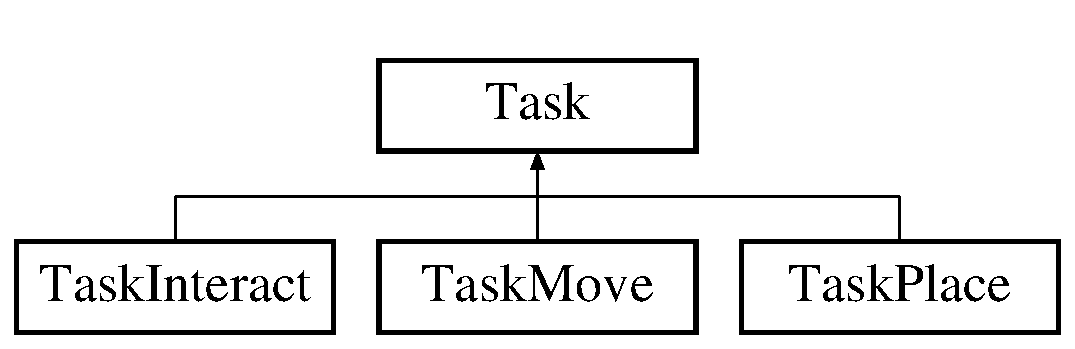
\includegraphics[height=2.000000cm]{classTask}
\end{center}
\end{figure}
\subsection*{Public Member Functions}
\begin{DoxyCompactItemize}
\item 
\hyperlink{classTask_abf784be50708a30e505f06e95205b326}{Task} (\hyperlink{classShipMaster}{Ship\-Master} \&\hyperlink{classTask_af765f4e3eab35d064f5cf18506b7c9a2}{ship})
\item 
virtual void \hyperlink{classTask_a186a7a8e9fa7d9bbd8c9fd3bf742250f}{do\-Task} (\hyperlink{classPerson}{Person} \&person)=0
\item 
bool \hyperlink{classTask_ae74007e9c8f09fea6504fd7c18550b9a}{walk\-One\-Step} (\hyperlink{classPerson}{Person} \&person)
\item 
void \hyperlink{classTask_a4090ed9b1ff941f0e284df65007a0dbc}{set\-Path} (\hyperlink{classPath}{Path} \hyperlink{classTask_a31352b3b35827e5898ceb39332fb1d77}{path})
\item 
void \hyperlink{classTask_a488b0f976e503b6af2dcc8cbfedbe6d8}{set\-Finished} (bool val)
\item 
bool \hyperlink{classTask_aa8013289fde3086e1c8816f65ed9298e}{is\-Finished} ()
\item 
bool \hyperlink{classTask_a096a6563f747c3b5f62bc4cf55efa37d}{has\-Path} ()
\end{DoxyCompactItemize}
\subsection*{Public Attributes}
\begin{DoxyCompactItemize}
\item 
bool \hyperlink{classTask_a81aa161cc48dc53e86b3d8dfa9d5dfe7}{finished}
\item 
\hyperlink{classPath}{Path} \hyperlink{classTask_a31352b3b35827e5898ceb39332fb1d77}{path}
\item 
\hyperlink{classShipMaster}{Ship\-Master} \& \hyperlink{classTask_af765f4e3eab35d064f5cf18506b7c9a2}{ship}
\end{DoxyCompactItemize}


\subsection{Constructor \& Destructor Documentation}
\hypertarget{classTask_abf784be50708a30e505f06e95205b326}{\index{Task@{Task}!Task@{Task}}
\index{Task@{Task}!Task@{Task}}
\subsubsection[{Task}]{\setlength{\rightskip}{0pt plus 5cm}Task\-::\-Task (
\begin{DoxyParamCaption}
\item[{{\bf Ship\-Master} \&}]{ship}
\end{DoxyParamCaption}
)\hspace{0.3cm}{\ttfamily [inline]}}}\label{classTask_abf784be50708a30e505f06e95205b326}


\subsection{Member Function Documentation}
\hypertarget{classTask_a186a7a8e9fa7d9bbd8c9fd3bf742250f}{\index{Task@{Task}!do\-Task@{do\-Task}}
\index{do\-Task@{do\-Task}!Task@{Task}}
\subsubsection[{do\-Task}]{\setlength{\rightskip}{0pt plus 5cm}virtual void Task\-::do\-Task (
\begin{DoxyParamCaption}
\item[{{\bf Person} \&}]{person}
\end{DoxyParamCaption}
)\hspace{0.3cm}{\ttfamily [pure virtual]}}}\label{classTask_a186a7a8e9fa7d9bbd8c9fd3bf742250f}


Implemented in \hyperlink{classTaskInteract_ae70faf65b992b6d6d6a32597b3b2ecec}{Task\-Interact}, \hyperlink{classTaskPlace_ac5edec0398ebab6ec06908a5d45162ef}{Task\-Place}, and \hyperlink{classTaskMove_a89ecbe18c5db0ba78a375cd0fda9daf8}{Task\-Move}.

\hypertarget{classTask_a096a6563f747c3b5f62bc4cf55efa37d}{\index{Task@{Task}!has\-Path@{has\-Path}}
\index{has\-Path@{has\-Path}!Task@{Task}}
\subsubsection[{has\-Path}]{\setlength{\rightskip}{0pt plus 5cm}bool Task\-::has\-Path (
\begin{DoxyParamCaption}
{}
\end{DoxyParamCaption}
)}}\label{classTask_a096a6563f747c3b5f62bc4cf55efa37d}
\hypertarget{classTask_aa8013289fde3086e1c8816f65ed9298e}{\index{Task@{Task}!is\-Finished@{is\-Finished}}
\index{is\-Finished@{is\-Finished}!Task@{Task}}
\subsubsection[{is\-Finished}]{\setlength{\rightskip}{0pt plus 5cm}bool Task\-::is\-Finished (
\begin{DoxyParamCaption}
{}
\end{DoxyParamCaption}
)}}\label{classTask_aa8013289fde3086e1c8816f65ed9298e}
\hypertarget{classTask_a488b0f976e503b6af2dcc8cbfedbe6d8}{\index{Task@{Task}!set\-Finished@{set\-Finished}}
\index{set\-Finished@{set\-Finished}!Task@{Task}}
\subsubsection[{set\-Finished}]{\setlength{\rightskip}{0pt plus 5cm}void Task\-::set\-Finished (
\begin{DoxyParamCaption}
\item[{bool}]{val}
\end{DoxyParamCaption}
)}}\label{classTask_a488b0f976e503b6af2dcc8cbfedbe6d8}
\hypertarget{classTask_a4090ed9b1ff941f0e284df65007a0dbc}{\index{Task@{Task}!set\-Path@{set\-Path}}
\index{set\-Path@{set\-Path}!Task@{Task}}
\subsubsection[{set\-Path}]{\setlength{\rightskip}{0pt plus 5cm}void Task\-::set\-Path (
\begin{DoxyParamCaption}
\item[{{\bf Path}}]{path}
\end{DoxyParamCaption}
)}}\label{classTask_a4090ed9b1ff941f0e284df65007a0dbc}
\hypertarget{classTask_ae74007e9c8f09fea6504fd7c18550b9a}{\index{Task@{Task}!walk\-One\-Step@{walk\-One\-Step}}
\index{walk\-One\-Step@{walk\-One\-Step}!Task@{Task}}
\subsubsection[{walk\-One\-Step}]{\setlength{\rightskip}{0pt plus 5cm}bool Task\-::walk\-One\-Step (
\begin{DoxyParamCaption}
\item[{{\bf Person} \&}]{person}
\end{DoxyParamCaption}
)}}\label{classTask_ae74007e9c8f09fea6504fd7c18550b9a}


\subsection{Member Data Documentation}
\hypertarget{classTask_a81aa161cc48dc53e86b3d8dfa9d5dfe7}{\index{Task@{Task}!finished@{finished}}
\index{finished@{finished}!Task@{Task}}
\subsubsection[{finished}]{\setlength{\rightskip}{0pt plus 5cm}bool Task\-::finished}}\label{classTask_a81aa161cc48dc53e86b3d8dfa9d5dfe7}
\hypertarget{classTask_a31352b3b35827e5898ceb39332fb1d77}{\index{Task@{Task}!path@{path}}
\index{path@{path}!Task@{Task}}
\subsubsection[{path}]{\setlength{\rightskip}{0pt plus 5cm}{\bf Path} Task\-::path}}\label{classTask_a31352b3b35827e5898ceb39332fb1d77}
\hypertarget{classTask_af765f4e3eab35d064f5cf18506b7c9a2}{\index{Task@{Task}!ship@{ship}}
\index{ship@{ship}!Task@{Task}}
\subsubsection[{ship}]{\setlength{\rightskip}{0pt plus 5cm}{\bf Ship\-Master}\& Task\-::ship}}\label{classTask_af765f4e3eab35d064f5cf18506b7c9a2}


The documentation for this class was generated from the following files\-:\begin{DoxyCompactItemize}
\item 
core/jobs/\hyperlink{Task_8h}{Task.\-h}\item 
core/jobs/\hyperlink{Task_8cpp}{Task.\-cpp}\end{DoxyCompactItemize}

\hypertarget{classTaskInteract}{\section{Task\-Interact Class Reference}
\label{classTaskInteract}\index{Task\-Interact@{Task\-Interact}}
}


{\ttfamily \#include $<$Task\-Interact.\-h$>$}

Inheritance diagram for Task\-Interact\-:\begin{figure}[H]
\begin{center}
\leavevmode
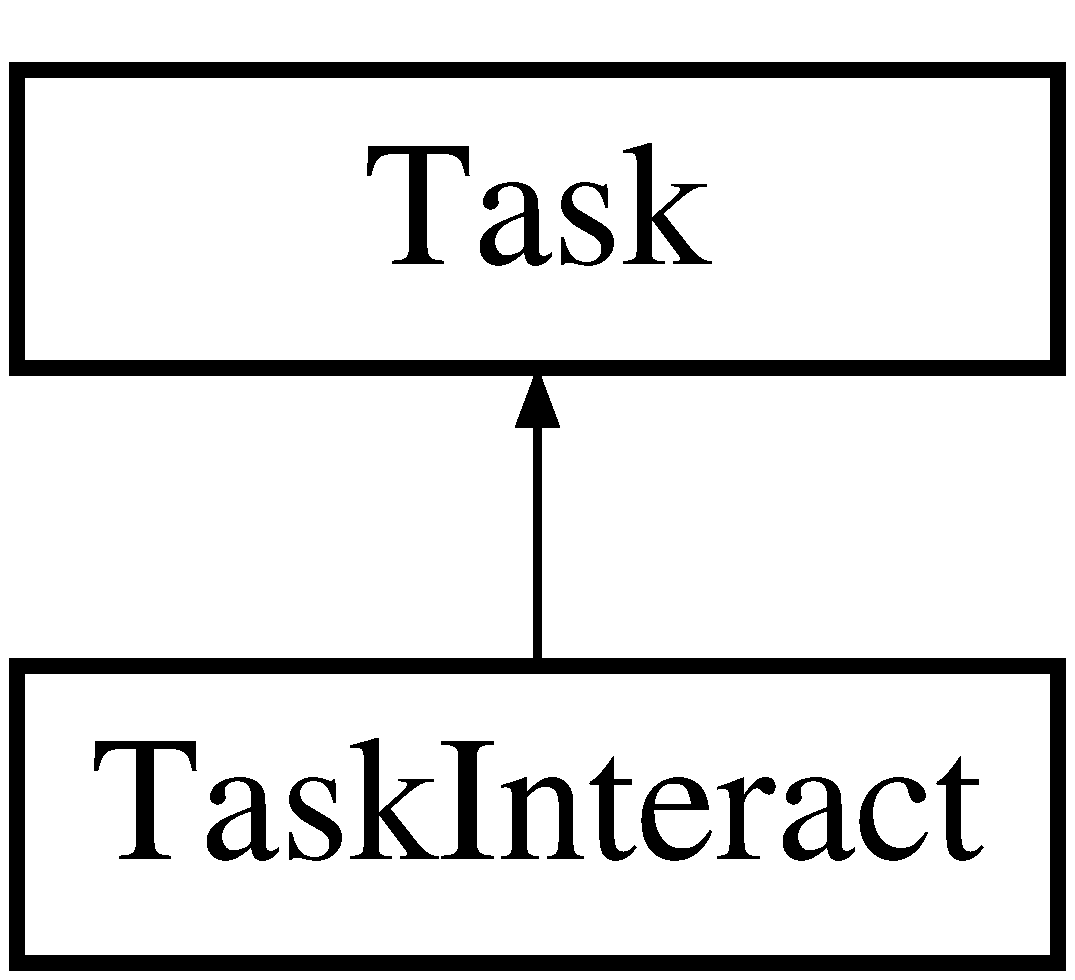
\includegraphics[height=2.000000cm]{classTaskInteract}
\end{center}
\end{figure}
\subsection*{Public Member Functions}
\begin{DoxyCompactItemize}
\item 
\hyperlink{classTaskInteract_a4c3bd10b67882eca11b6d60d77441d78}{Task\-Interact} (\hyperlink{classItem}{Item} $\ast$obj, \hyperlink{classShipMaster}{Ship\-Master} \&\hyperlink{classTask_af765f4e3eab35d064f5cf18506b7c9a2}{ship}, \hyperlink{structLocation}{Location} current\-Pos)
\item 
void \hyperlink{classTaskInteract_ae70faf65b992b6d6d6a32597b3b2ecec}{do\-Task} (\hyperlink{classPerson}{Person} \&person)
\item 
void \hyperlink{classTaskInteract_ad628c33366242e400734bddd4b120104}{set\-Item} (\hyperlink{classItem}{Item} $\ast$object)
\end{DoxyCompactItemize}
\subsection*{Public Attributes}
\begin{DoxyCompactItemize}
\item 
\hyperlink{classItem}{Item} $\ast$ \hyperlink{classTaskInteract_ab84e9122334cfd0e1a32eac3bbba2e2d}{target}
\end{DoxyCompactItemize}


\subsection{Constructor \& Destructor Documentation}
\hypertarget{classTaskInteract_a4c3bd10b67882eca11b6d60d77441d78}{\index{Task\-Interact@{Task\-Interact}!Task\-Interact@{Task\-Interact}}
\index{Task\-Interact@{Task\-Interact}!TaskInteract@{Task\-Interact}}
\subsubsection[{Task\-Interact}]{\setlength{\rightskip}{0pt plus 5cm}Task\-Interact\-::\-Task\-Interact (
\begin{DoxyParamCaption}
\item[{{\bf Item} $\ast$}]{obj, }
\item[{{\bf Ship\-Master} \&}]{ship, }
\item[{{\bf Location}}]{current\-Pos}
\end{DoxyParamCaption}
)}}\label{classTaskInteract_a4c3bd10b67882eca11b6d60d77441d78}


\subsection{Member Function Documentation}
\hypertarget{classTaskInteract_ae70faf65b992b6d6d6a32597b3b2ecec}{\index{Task\-Interact@{Task\-Interact}!do\-Task@{do\-Task}}
\index{do\-Task@{do\-Task}!TaskInteract@{Task\-Interact}}
\subsubsection[{do\-Task}]{\setlength{\rightskip}{0pt plus 5cm}void Task\-Interact\-::do\-Task (
\begin{DoxyParamCaption}
\item[{{\bf Person} \&}]{person}
\end{DoxyParamCaption}
)\hspace{0.3cm}{\ttfamily [virtual]}}}\label{classTaskInteract_ae70faf65b992b6d6d6a32597b3b2ecec}


Implements \hyperlink{classTask_a186a7a8e9fa7d9bbd8c9fd3bf742250f}{Task}.

\hypertarget{classTaskInteract_ad628c33366242e400734bddd4b120104}{\index{Task\-Interact@{Task\-Interact}!set\-Item@{set\-Item}}
\index{set\-Item@{set\-Item}!TaskInteract@{Task\-Interact}}
\subsubsection[{set\-Item}]{\setlength{\rightskip}{0pt plus 5cm}void Task\-Interact\-::set\-Item (
\begin{DoxyParamCaption}
\item[{{\bf Item} $\ast$}]{object}
\end{DoxyParamCaption}
)}}\label{classTaskInteract_ad628c33366242e400734bddd4b120104}


\subsection{Member Data Documentation}
\hypertarget{classTaskInteract_ab84e9122334cfd0e1a32eac3bbba2e2d}{\index{Task\-Interact@{Task\-Interact}!target@{target}}
\index{target@{target}!TaskInteract@{Task\-Interact}}
\subsubsection[{target}]{\setlength{\rightskip}{0pt plus 5cm}{\bf Item}$\ast$ Task\-Interact\-::target}}\label{classTaskInteract_ab84e9122334cfd0e1a32eac3bbba2e2d}


The documentation for this class was generated from the following files\-:\begin{DoxyCompactItemize}
\item 
core/jobs/\hyperlink{TaskInteract_8h}{Task\-Interact.\-h}\item 
core/jobs/\hyperlink{TaskInteract_8cpp}{Task\-Interact.\-cpp}\end{DoxyCompactItemize}

\hypertarget{classTaskMove}{\section{Task\-Move Class Reference}
\label{classTaskMove}\index{Task\-Move@{Task\-Move}}
}


{\ttfamily \#include $<$Task\-Move.\-h$>$}

Inheritance diagram for Task\-Move\-:\begin{figure}[H]
\begin{center}
\leavevmode
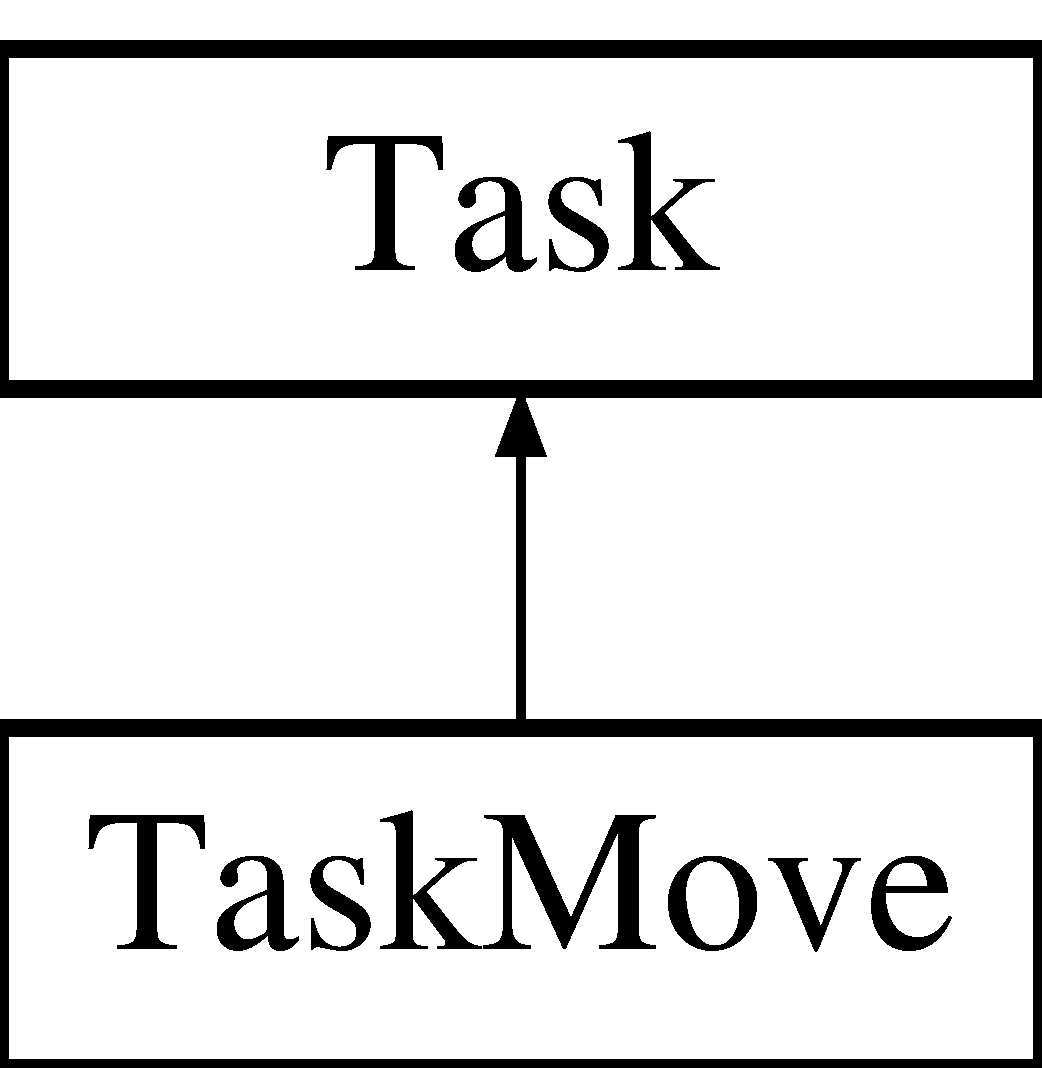
\includegraphics[height=2.000000cm]{classTaskMove}
\end{center}
\end{figure}
\subsection*{Public Member Functions}
\begin{DoxyCompactItemize}
\item 
\hyperlink{classTaskMove_abb70657171621a529de87daf5ca740cb}{Task\-Move} (\hyperlink{classShipMaster}{Ship\-Master} \&\hyperlink{classTask_af765f4e3eab35d064f5cf18506b7c9a2}{ship}, \hyperlink{structLocation}{Location} current\-Pos, \hyperlink{structLocation}{Location} end)
\item 
void \hyperlink{classTaskMove_a89ecbe18c5db0ba78a375cd0fda9daf8}{do\-Task} (\hyperlink{classPerson}{Person} \&person)
\end{DoxyCompactItemize}
\subsection*{Additional Inherited Members}


\subsection{Constructor \& Destructor Documentation}
\hypertarget{classTaskMove_abb70657171621a529de87daf5ca740cb}{\index{Task\-Move@{Task\-Move}!Task\-Move@{Task\-Move}}
\index{Task\-Move@{Task\-Move}!TaskMove@{Task\-Move}}
\subsubsection[{Task\-Move}]{\setlength{\rightskip}{0pt plus 5cm}Task\-Move\-::\-Task\-Move (
\begin{DoxyParamCaption}
\item[{{\bf Ship\-Master} \&}]{ship, }
\item[{{\bf Location}}]{current\-Pos, }
\item[{{\bf Location}}]{end}
\end{DoxyParamCaption}
)}}\label{classTaskMove_abb70657171621a529de87daf5ca740cb}


\subsection{Member Function Documentation}
\hypertarget{classTaskMove_a89ecbe18c5db0ba78a375cd0fda9daf8}{\index{Task\-Move@{Task\-Move}!do\-Task@{do\-Task}}
\index{do\-Task@{do\-Task}!TaskMove@{Task\-Move}}
\subsubsection[{do\-Task}]{\setlength{\rightskip}{0pt plus 5cm}void Task\-Move\-::do\-Task (
\begin{DoxyParamCaption}
\item[{{\bf Person} \&}]{person}
\end{DoxyParamCaption}
)\hspace{0.3cm}{\ttfamily [virtual]}}}\label{classTaskMove_a89ecbe18c5db0ba78a375cd0fda9daf8}


Implements \hyperlink{classTask_a186a7a8e9fa7d9bbd8c9fd3bf742250f}{Task}.



The documentation for this class was generated from the following files\-:\begin{DoxyCompactItemize}
\item 
core/jobs/\hyperlink{TaskMove_8h}{Task\-Move.\-h}\item 
core/jobs/\hyperlink{TaskMove_8cpp}{Task\-Move.\-cpp}\end{DoxyCompactItemize}

\hypertarget{classTaskPlace}{\section{Task\-Place Class Reference}
\label{classTaskPlace}\index{Task\-Place@{Task\-Place}}
}


{\ttfamily \#include $<$Task\-Place.\-h$>$}

Inheritance diagram for Task\-Place\-:\begin{figure}[H]
\begin{center}
\leavevmode
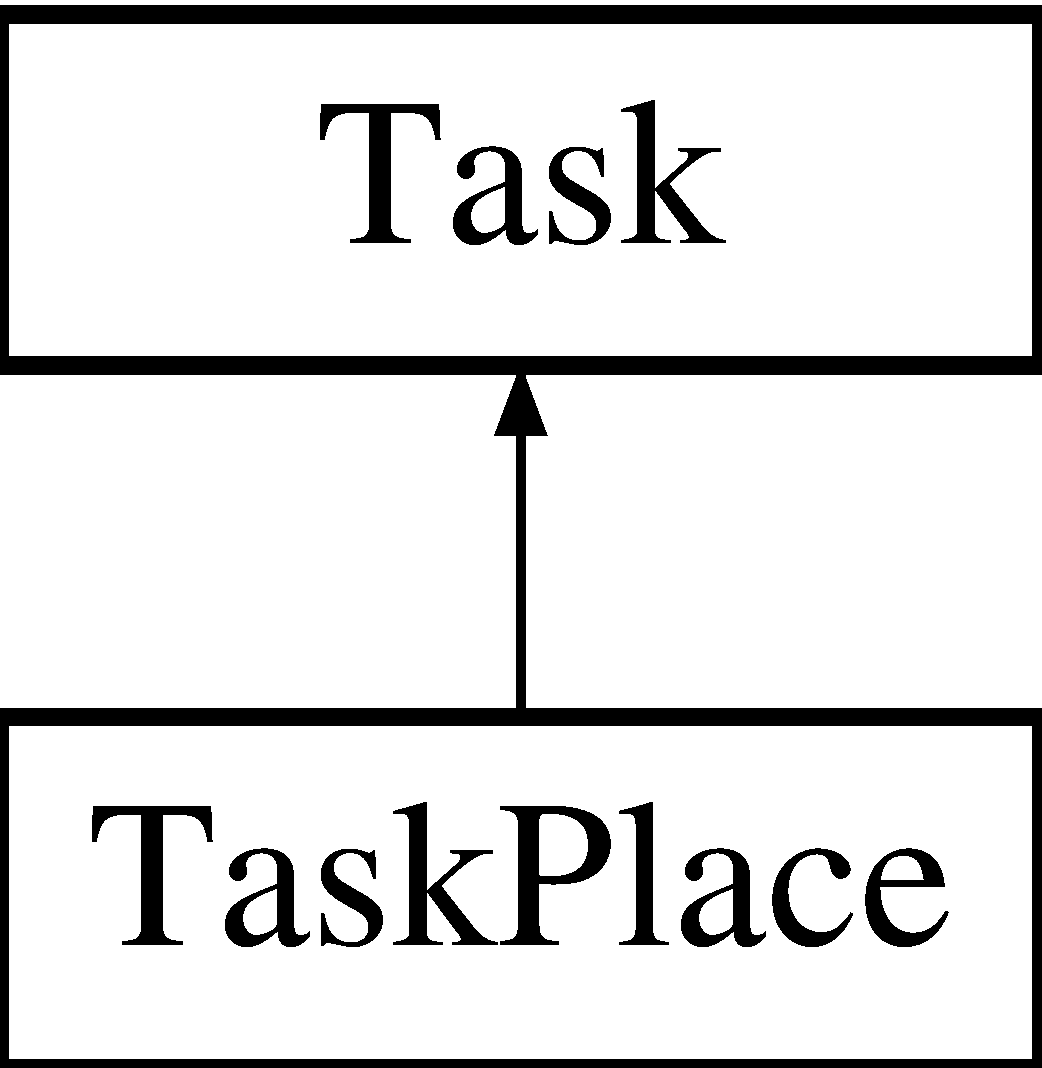
\includegraphics[height=2.000000cm]{classTaskPlace}
\end{center}
\end{figure}
\subsection*{Public Member Functions}
\begin{DoxyCompactItemize}
\item 
\hyperlink{classTaskPlace_ac2d6925c81a4004bc5d50ed79c3a8c05}{Task\-Place} (\hyperlink{classItem}{Item} $\ast$\hyperlink{classTaskPlace_ad90f2f82f39289bbaeaef5982831d369}{obj}, \hyperlink{classShipMaster}{Ship\-Master} \&\hyperlink{classTask_af765f4e3eab35d064f5cf18506b7c9a2}{ship}, \hyperlink{structLocation}{Location} current\-Pos)
\item 
void \hyperlink{classTaskPlace_ac5edec0398ebab6ec06908a5d45162ef}{do\-Task} (\hyperlink{classPerson}{Person} \&person)
\end{DoxyCompactItemize}
\subsection*{Public Attributes}
\begin{DoxyCompactItemize}
\item 
\hyperlink{classItem}{Item} $\ast$ \hyperlink{classTaskPlace_ad90f2f82f39289bbaeaef5982831d369}{obj}
\end{DoxyCompactItemize}


\subsection{Constructor \& Destructor Documentation}
\hypertarget{classTaskPlace_ac2d6925c81a4004bc5d50ed79c3a8c05}{\index{Task\-Place@{Task\-Place}!Task\-Place@{Task\-Place}}
\index{Task\-Place@{Task\-Place}!TaskPlace@{Task\-Place}}
\subsubsection[{Task\-Place}]{\setlength{\rightskip}{0pt plus 5cm}Task\-Place\-::\-Task\-Place (
\begin{DoxyParamCaption}
\item[{{\bf Item} $\ast$}]{obj, }
\item[{{\bf Ship\-Master} \&}]{ship, }
\item[{{\bf Location}}]{current\-Pos}
\end{DoxyParamCaption}
)}}\label{classTaskPlace_ac2d6925c81a4004bc5d50ed79c3a8c05}


\subsection{Member Function Documentation}
\hypertarget{classTaskPlace_ac5edec0398ebab6ec06908a5d45162ef}{\index{Task\-Place@{Task\-Place}!do\-Task@{do\-Task}}
\index{do\-Task@{do\-Task}!TaskPlace@{Task\-Place}}
\subsubsection[{do\-Task}]{\setlength{\rightskip}{0pt plus 5cm}void Task\-Place\-::do\-Task (
\begin{DoxyParamCaption}
\item[{{\bf Person} \&}]{person}
\end{DoxyParamCaption}
)\hspace{0.3cm}{\ttfamily [virtual]}}}\label{classTaskPlace_ac5edec0398ebab6ec06908a5d45162ef}


Implements \hyperlink{classTask_a186a7a8e9fa7d9bbd8c9fd3bf742250f}{Task}.



\subsection{Member Data Documentation}
\hypertarget{classTaskPlace_ad90f2f82f39289bbaeaef5982831d369}{\index{Task\-Place@{Task\-Place}!obj@{obj}}
\index{obj@{obj}!TaskPlace@{Task\-Place}}
\subsubsection[{obj}]{\setlength{\rightskip}{0pt plus 5cm}{\bf Item}$\ast$ Task\-Place\-::obj}}\label{classTaskPlace_ad90f2f82f39289bbaeaef5982831d369}


The documentation for this class was generated from the following files\-:\begin{DoxyCompactItemize}
\item 
core/jobs/\hyperlink{TaskPlace_8h}{Task\-Place.\-h}\item 
core/jobs/\hyperlink{TaskPlace_8cpp}{Task\-Place.\-cpp}\end{DoxyCompactItemize}

\hypertarget{classWeaponry}{\section{Weaponry Class Reference}
\label{classWeaponry}\index{Weaponry@{Weaponry}}
}


Parent class for weapon blocks that can fire on an enemy ship.  




{\ttfamily \#include $<$Weaponry.\-h$>$}

Inheritance diagram for Weaponry\-:\begin{figure}[H]
\begin{center}
\leavevmode
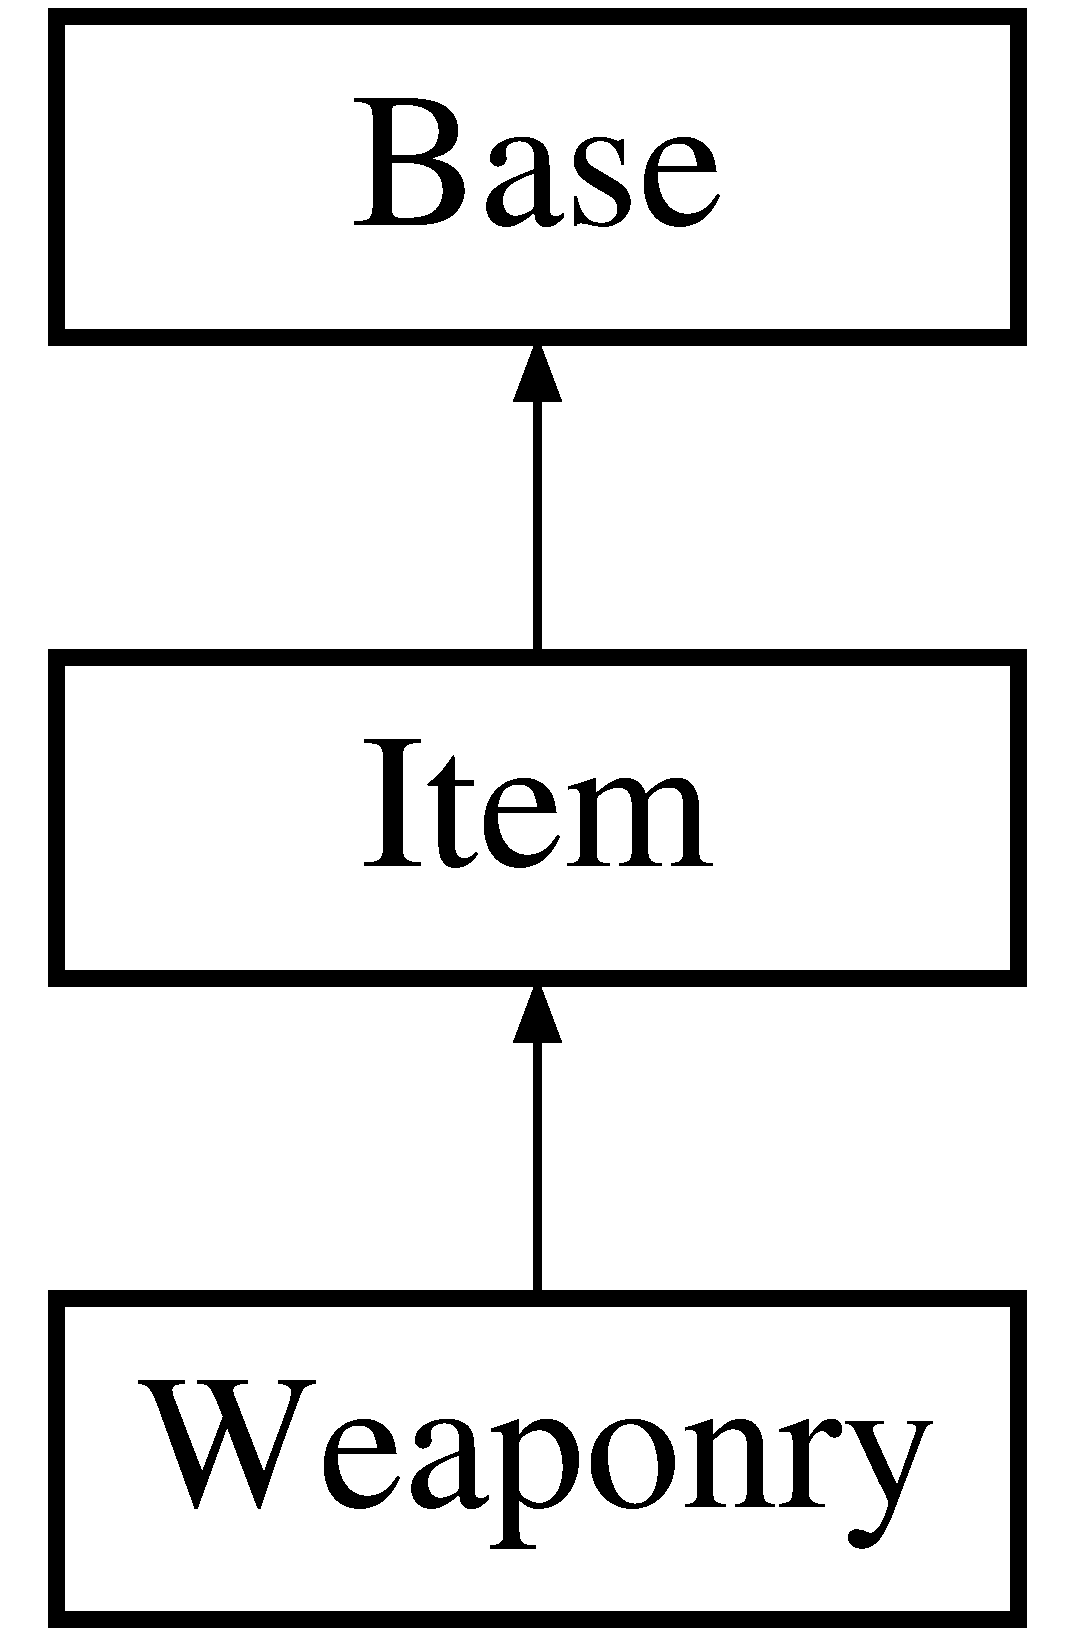
\includegraphics[height=3.000000cm]{classWeaponry}
\end{center}
\end{figure}
\subsection*{Public Member Functions}
\begin{DoxyCompactItemize}
\item 
\hyperlink{classWeaponry_a4a16e01bf2e344703c502020931e0cda}{Weaponry} (int \hyperlink{classBase_a1dddc037afe2eae3e1364597e6a3cf46}{I\-D}, int \hyperlink{classItem_adcfbfc3a87d2112c62b812dac2c72993}{slot}, int \hyperlink{classItem_a5166900b24ba9e746a7ad34c00353cdd}{blocking})
\item 
virtual void \hyperlink{classWeaponry_a25e7854098914225b10722fccbe7a3a8}{get\-Targets} (\hyperlink{structLocation}{Location} $\ast$\hyperlink{classItem_ade907eeeea58df68fcacde1e5568779b}{loc}, int \&N)=0
\begin{DoxyCompactList}\small\item\em Get locations of where the weapon is targeting. \end{DoxyCompactList}\item 
virtual void \hyperlink{classWeaponry_a65e4ba85708c33bf0a6b138e7db19e69}{get\-Damage} (int target\-Type)=0
\begin{DoxyCompactList}\small\item\em Get the amount of damage given the spesific target type. \end{DoxyCompactList}\item 
virtual void \hyperlink{classWeaponry_abf73f52293778d70c1639a7f866f0e86}{get\-Damage\-Type} ()=0
\begin{DoxyCompactList}\small\item\em Get the identifier of the type of weapon damage. \end{DoxyCompactList}\end{DoxyCompactItemize}
\subsection*{Additional Inherited Members}


\subsection{Detailed Description}
Parent class for weapon blocks that can fire on an enemy ship. 

Objects that are ment to fire on enemy ships should inherit this class to be integrated correctly into the ship system. Overriding the virtual methods ensures the weapon can be handled by the system. 

\subsection{Constructor \& Destructor Documentation}
\hypertarget{classWeaponry_a4a16e01bf2e344703c502020931e0cda}{\index{Weaponry@{Weaponry}!Weaponry@{Weaponry}}
\index{Weaponry@{Weaponry}!Weaponry@{Weaponry}}
\subsubsection[{Weaponry}]{\setlength{\rightskip}{0pt plus 5cm}Weaponry\-::\-Weaponry (
\begin{DoxyParamCaption}
\item[{int}]{I\-D, }
\item[{int}]{slot, }
\item[{int}]{blocking}
\end{DoxyParamCaption}
)\hspace{0.3cm}{\ttfamily [inline]}}}\label{classWeaponry_a4a16e01bf2e344703c502020931e0cda}


\subsection{Member Function Documentation}
\hypertarget{classWeaponry_a65e4ba85708c33bf0a6b138e7db19e69}{\index{Weaponry@{Weaponry}!get\-Damage@{get\-Damage}}
\index{get\-Damage@{get\-Damage}!Weaponry@{Weaponry}}
\subsubsection[{get\-Damage}]{\setlength{\rightskip}{0pt plus 5cm}virtual void Weaponry\-::get\-Damage (
\begin{DoxyParamCaption}
\item[{int}]{target\-Type}
\end{DoxyParamCaption}
)\hspace{0.3cm}{\ttfamily [pure virtual]}}}\label{classWeaponry_a65e4ba85708c33bf0a6b138e7db19e69}


Get the amount of damage given the spesific target type. 

E.\-g. A plasma laser might do more damage to shields. 
\begin{DoxyParams}{Parameters}
{\em target\-Type} & Target type identifier. \\
\hline
\end{DoxyParams}
\begin{DoxySeeAlso}{See Also}
\hyperlink{identifiers_8h}{identifiers.\-h} 
\end{DoxySeeAlso}
\hypertarget{classWeaponry_abf73f52293778d70c1639a7f866f0e86}{\index{Weaponry@{Weaponry}!get\-Damage\-Type@{get\-Damage\-Type}}
\index{get\-Damage\-Type@{get\-Damage\-Type}!Weaponry@{Weaponry}}
\subsubsection[{get\-Damage\-Type}]{\setlength{\rightskip}{0pt plus 5cm}virtual void Weaponry\-::get\-Damage\-Type (
\begin{DoxyParamCaption}
{}
\end{DoxyParamCaption}
)\hspace{0.3cm}{\ttfamily [pure virtual]}}}\label{classWeaponry_abf73f52293778d70c1639a7f866f0e86}


Get the identifier of the type of weapon damage. 

This can effect how the damage is received by the target hit. \hypertarget{classWeaponry_a25e7854098914225b10722fccbe7a3a8}{\index{Weaponry@{Weaponry}!get\-Targets@{get\-Targets}}
\index{get\-Targets@{get\-Targets}!Weaponry@{Weaponry}}
\subsubsection[{get\-Targets}]{\setlength{\rightskip}{0pt plus 5cm}virtual void Weaponry\-::get\-Targets (
\begin{DoxyParamCaption}
\item[{{\bf Location} $\ast$}]{loc, }
\item[{int \&}]{N}
\end{DoxyParamCaption}
)\hspace{0.3cm}{\ttfamily [pure virtual]}}}\label{classWeaponry_a25e7854098914225b10722fccbe7a3a8}


Get locations of where the weapon is targeting. 


\begin{DoxyParams}{Parameters}
{\em loc} & Output list of target locations. \\
\hline
{\em N} & Output number of target locations. \\
\hline
\end{DoxyParams}


The documentation for this class was generated from the following file\-:\begin{DoxyCompactItemize}
\item 
core/items/\hyperlink{Weaponry_8h}{Weaponry.\-h}\end{DoxyCompactItemize}

\chapter{File Documentation}
\hypertarget{AppDelegate_8cpp}{\section{App\-Delegate.\-cpp File Reference}
\label{AppDelegate_8cpp}\index{App\-Delegate.\-cpp@{App\-Delegate.\-cpp}}
}
{\ttfamily \#include \char`\"{}App\-Delegate.\-h\char`\"{}}\\*
{\ttfamily \#include \char`\"{}Hello\-World\-Scene.\-h\char`\"{}}\\*
\subsection*{Variables}
\begin{DoxyCompactItemize}
\item 
\hyperlink{AppDelegate_8cpp_ac10da2fd6444e5c9f74c64c543c0d747}{U\-S\-I\-N\-G\-\_\-\-N\-S\-\_\-\-C\-C}
\end{DoxyCompactItemize}


\subsection{Variable Documentation}
\hypertarget{AppDelegate_8cpp_ac10da2fd6444e5c9f74c64c543c0d747}{\index{App\-Delegate.\-cpp@{App\-Delegate.\-cpp}!U\-S\-I\-N\-G\-\_\-\-N\-S\-\_\-\-C\-C@{U\-S\-I\-N\-G\-\_\-\-N\-S\-\_\-\-C\-C}}
\index{U\-S\-I\-N\-G\-\_\-\-N\-S\-\_\-\-C\-C@{U\-S\-I\-N\-G\-\_\-\-N\-S\-\_\-\-C\-C}!AppDelegate.cpp@{App\-Delegate.\-cpp}}
\subsubsection[{U\-S\-I\-N\-G\-\_\-\-N\-S\-\_\-\-C\-C}]{\setlength{\rightskip}{0pt plus 5cm}U\-S\-I\-N\-G\-\_\-\-N\-S\-\_\-\-C\-C}}\label{AppDelegate_8cpp_ac10da2fd6444e5c9f74c64c543c0d747}

\hypertarget{AppDelegate_8h}{\section{App\-Delegate.\-h File Reference}
\label{AppDelegate_8h}\index{App\-Delegate.\-h@{App\-Delegate.\-h}}
}
{\ttfamily \#include \char`\"{}cocos2d.\-h\char`\"{}}\\*
\subsection*{Classes}
\begin{DoxyCompactItemize}
\item 
class \hyperlink{classAppDelegate}{App\-Delegate}
\begin{DoxyCompactList}\small\item\em The cocos2d Application. \end{DoxyCompactList}\end{DoxyCompactItemize}

\hypertarget{Base_8cpp}{\section{core/\-Base.cpp File Reference}
\label{Base_8cpp}\index{core/\-Base.\-cpp@{core/\-Base.\-cpp}}
}
{\ttfamily \#include \char`\"{}Base.\-h\char`\"{}}\\*

\hypertarget{Base_8h}{\section{core/\-Base.h File Reference}
\label{Base_8h}\index{core/\-Base.\-h@{core/\-Base.\-h}}
}
\subsection*{Classes}
\begin{DoxyCompactItemize}
\item 
class \hyperlink{classBase}{Base}
\begin{DoxyCompactList}\small\item\em All objects which have an I\-D and U\-I\-D inherit from \hyperlink{classBase}{Base}. \end{DoxyCompactList}\end{DoxyCompactItemize}

\hypertarget{core_8dox}{\section{core/core.dox File Reference}
\label{core_8dox}\index{core/core.\-dox@{core/core.\-dox}}
}

\hypertarget{Person_8cpp}{\section{core/enteties/\-Person.cpp File Reference}
\label{Person_8cpp}\index{core/enteties/\-Person.\-cpp@{core/enteties/\-Person.\-cpp}}
}
{\ttfamily \#include \char`\"{}../\-Base.\-h\char`\"{}}\\*
{\ttfamily \#include \char`\"{}../jobs/\-Task.\-h\char`\"{}}\\*
{\ttfamily \#include \char`\"{}Person.\-h\char`\"{}}\\*
{\ttfamily \#include $<$iostream$>$}\\*

\hypertarget{Person_8h}{\section{core/enteties/\-Person.h File Reference}
\label{Person_8h}\index{core/enteties/\-Person.\-h@{core/enteties/\-Person.\-h}}
}
{\ttfamily \#include \char`\"{}../\-Base.\-h\char`\"{}}\\*
{\ttfamily \#include \char`\"{}../map/\-Location.\-h\char`\"{}}\\*
\subsection*{Classes}
\begin{DoxyCompactItemize}
\item 
class \hyperlink{classPerson}{Person}
\end{DoxyCompactItemize}

\hypertarget{identifiers_8h}{\section{core/identifiers.h File Reference}
\label{identifiers_8h}\index{core/identifiers.\-h@{core/identifiers.\-h}}
}
\subsection*{Namespaces}
\begin{DoxyCompactItemize}
\item 
\hyperlink{namespaceglobals}{globals}
\begin{DoxyCompactList}\small\item\em Global values. \end{DoxyCompactList}\item 
\hyperlink{namespacedirections}{directions}
\begin{DoxyCompactList}\small\item\em Direction identifiers. \end{DoxyCompactList}\item 
\hyperlink{namespacetextures}{textures}
\begin{DoxyCompactList}\small\item\em Texture I\-Ds.

Each id represents the U\-I\-D of a tile in the tilset. This should match the U\-I\-D in Tiled. \end{DoxyCompactList}\item 
\hyperlink{namespacerooms}{rooms}
\begin{DoxyCompactList}\small\item\em \hyperlink{classRoom}{Room} I\-Ds. \end{DoxyCompactList}\item 
\hyperlink{namespaceblocks}{blocks}
\begin{DoxyCompactList}\small\item\em Contains item I\-Ds, and property specifiers.

Contains all item I\-Ds as well as flags for specifying if. \end{DoxyCompactList}\end{DoxyCompactItemize}
\subsection*{Variables}
\begin{DoxyCompactItemize}
\item 
const int \hyperlink{namespaceglobals_ad06f2af5cf1c7c3b13ea34b6f0903af0}{globals\-::\-M\-A\-X\-\_\-\-P\-A\-T\-H\-\_\-\-L\-E\-N\-G\-T\-H} = 20
\begin{DoxyCompactList}\small\item\em Maximum path length return from the pathfinding algorithm. \end{DoxyCompactList}\item 
const int \hyperlink{namespaceglobals_a3209a1ea09047e47023bbe9982b4945b}{globals\-::\-M\-A\-X\-\_\-\-C\-R\-E\-W} = 100
\begin{DoxyCompactList}\small\item\em Maximum number of actors in the local world. \end{DoxyCompactList}\item 
const int \hyperlink{namespacedirections_ae9cfa895df6c71a9a932353c2d698748}{directions\-::\-D\-I\-R\-E\-C\-T\-I\-O\-N\-S} = 6
\begin{DoxyCompactList}\small\item\em Number of directions. \end{DoxyCompactList}\item 
const unsigned int \hyperlink{namespacedirections_a07f0f35a8e192bdbfbe343b4cc3ac5f0}{directions\-::\-N\-O\-\_\-\-D\-I\-R\-E\-C\-T\-I\-O\-N} = 0
\item 
const unsigned int \hyperlink{namespacedirections_aaac74a9680a4a4485ea7966d9cc1e7a0}{directions\-::\-E\-A\-S\-T} = 1$<$$<$0
\item 
const unsigned int \hyperlink{namespacedirections_abe28a39304326df4cd876a6f8267b8a0}{directions\-::\-N\-O\-R\-T\-H} = 1$<$$<$1
\item 
const unsigned int \hyperlink{namespacedirections_a9164128a01e52cb46cea45b60d3e0d24}{directions\-::\-U\-P} = 1$<$$<$2
\item 
const unsigned int \hyperlink{namespacedirections_a6050c968985dc0ca37f492dbd9665b59}{directions\-::\-W\-E\-S\-T} = 1$<$$<$3
\item 
const unsigned int \hyperlink{namespacedirections_a01f808fbd532b480f6df835ba039eeb3}{directions\-::\-S\-O\-U\-T\-H} = 1$<$$<$4
\item 
const unsigned int \hyperlink{namespacedirections_ac5b0521b6f55c6c27dd493c816eaf61a}{directions\-::\-D\-O\-W\-N} = 1$<$$<$5
\item 
const unsigned int \hyperlink{namespacedirections_afb925db0683d3de68b06587ccc1be620}{directions\-::\-B\-L\-O\-C\-K\-\_\-\-N\-O\-N\-E} = 0
\item 
const unsigned int \hyperlink{namespacedirections_ad1c6d7e5b1f142442ae7a7d527281e9f}{directions\-::\-B\-L\-O\-C\-K\-\_\-\-W\-E\-S\-T} = 1$<$$<$0
\item 
const unsigned int \hyperlink{namespacedirections_a19a70e2862864e20ea8b52f15f18a4d4}{directions\-::\-B\-L\-O\-C\-K\-\_\-\-S\-O\-U\-T\-H} = 1$<$$<$1
\item 
const unsigned int \hyperlink{namespacedirections_aee5c7106d29fd47f5dedb475537fa6ad}{directions\-::\-B\-L\-O\-C\-K\-\_\-\-D\-O\-W\-N} = 1$<$$<$2
\item 
const unsigned int \hyperlink{namespacedirections_aeafc68d54c090e0e7fc49c20f75f6f71}{directions\-::\-B\-L\-O\-C\-K\-\_\-\-E\-A\-S\-T} = 1$<$$<$3
\item 
const unsigned int \hyperlink{namespacedirections_aafa10fc7e4d258d59153b41e0c3c3972}{directions\-::\-B\-L\-O\-C\-K\-\_\-\-N\-O\-R\-T\-H} = 1$<$$<$4
\item 
const unsigned int \hyperlink{namespacedirections_a75d6cf52d7c325364a0288afdc7affd8}{directions\-::\-B\-L\-O\-C\-K\-\_\-\-U\-P} = 1$<$$<$5
\item 
const unsigned int \hyperlink{namespacedirections_a3a3b00ffd9ec88e2780368bd7604e31b}{directions\-::\-B\-L\-O\-C\-K\-\_\-\-A\-L\-L}
\item 
const unsigned int \hyperlink{namespacetextures_a0441d01cbc4e61c26642f3ae2199ff01}{textures\-::\-N\-O\-\_\-\-T\-E\-X\-T\-U\-R\-E} = 0
\item 
const unsigned int \hyperlink{namespacetextures_ad9d822633e938b097758d935dbf7addf}{textures\-::\-C\-O\-R\-N\-\_\-\-T\-E\-X\-T\-U\-R\-E\-\_\-1} = 39
\item 
const unsigned int \hyperlink{namespacetextures_a4ea11f59a0eb308393ca4a67d75d8e1d}{textures\-::\-C\-O\-R\-N\-\_\-\-T\-E\-X\-T\-U\-R\-E\-\_\-2} = 38
\item 
const unsigned int \hyperlink{namespacetextures_a1b3b07f0dfd7b82f409765d6153bc641}{textures\-::\-C\-O\-R\-N\-\_\-\-T\-E\-X\-T\-U\-R\-E\-\_\-3} = 40
\item 
const int \hyperlink{namespacerooms_af442e0eb93ff764fd8719778cf57198c}{rooms\-::\-K\-I\-T\-C\-H\-E\-N} = 1
\item 
const int \hyperlink{namespacerooms_af6e6156e1e069732b4a871a08c0a0764}{rooms\-::\-B\-R\-I\-D\-G\-E} = 2
\item 
const int \hyperlink{namespacerooms_adb86c88291085e8000065eb5ded8d372}{rooms\-::\-E\-N\-G\-I\-N\-E} = 3
\item 
const int \hyperlink{namespacerooms_a70b442e599b3d5be772a5288cfc8ce71}{rooms\-::\-W\-E\-A\-P\-O\-N\-S} = 4
\item 
const unsigned int \hyperlink{namespaceblocks_a737c0542023b22bab8672250922590e6}{blocks\-::\-C\-E\-N\-T\-E\-R\-\_\-\-S\-P\-A\-C\-E} = 1
\item 
const unsigned int \hyperlink{namespaceblocks_a3327185e4957b8756fcd8b0aeae2cbcb}{blocks\-::\-C\-E\-N\-T\-E\-R\-\_\-\-A\-I\-R} = 2
\item 
const unsigned int \hyperlink{namespaceblocks_a32435f4674386fdba12f33155aea4310}{blocks\-::\-C\-E\-N\-T\-E\-R\-\_\-\-M\-E\-T\-A\-L} = 3
\item 
const unsigned int \hyperlink{namespaceblocks_a443c0848965126c5e669c5e88fd44426}{blocks\-::\-W\-A\-L\-L\-\_\-\-M\-E\-T\-A\-L} = 4
\item 
const unsigned int \hyperlink{namespaceblocks_a0b0352a68a2e1ee22c3fd2e94181d15d}{blocks\-::\-F\-L\-O\-O\-R\-\_\-\-M\-E\-T\-A\-L} = 5
\item 
const unsigned int \hyperlink{namespaceblocks_a447728bb17162a7d87ed06d4db11060a}{blocks\-::\-C\-E\-N\-T\-E\-R\-\_\-\-C\-O\-R\-N} = 6
\item 
const int \hyperlink{namespaceblocks_aea8b288e0f2f0df691ade96adb6f0833}{blocks\-::\-C\-O\-U\-N\-T} = 6
\item 
const int \hyperlink{namespaceblocks_a0493803a45dd00ed11cc9be729da4317}{blocks\-::\-N\-O\-N\-\_\-\-B\-L\-O\-C\-K\-I\-N\-G} = 0
\item 
const int \hyperlink{namespaceblocks_a12de5833d1f76be099d7371038e239cd}{blocks\-::\-B\-L\-O\-C\-K\-I\-N\-G} = 1
\item 
const int \hyperlink{namespaceblocks_a293bbaa7ca5f1014dc69c2caaa414095}{blocks\-::\-C\-E\-N\-T\-E\-R} = 0
\item 
const int \hyperlink{namespaceblocks_af99b22467101d71649b471215cc001fb}{blocks\-::\-F\-L\-O\-O\-R} = 1
\item 
const int \hyperlink{namespaceblocks_abc4e6acf8b46e7e8ef24cdc3e4f2a744}{blocks\-::\-W\-A\-L\-L} = 2
\item 
const int \hyperlink{namespaceblocks_a6bdd8efa1c06420d581b18dd63651633}{blocks\-::\-U\-N\-S\-P\-E\-C\-I\-F\-I\-E\-D} = 1
\item 
const int \hyperlink{namespaceblocks_a60a02114e9d8f1775ff2cd109606f78f}{blocks\-::\-W\-E\-A\-P\-O\-N\-R\-Y} = 2
\item 
const int \hyperlink{namespaceblocks_a4d5910f765824bac56f2737496e51a7d}{blocks\-::\-E\-N\-T\-E\-T\-Y} = 1
\item 
const int \hyperlink{namespaceblocks_a94050edf77a38898d8d81e0621a5cd62}{blocks\-::\-C\-O\-N\-S\-T\-R\-U\-C\-T} = 2
\item 
const int \hyperlink{namespaceblocks_a8a40b228670ab6718cd7678691a660e0}{blocks\-::\-C\-O\-N\-S\-T\-R\-U\-C\-T\-\_\-\-S\-O\-F\-T} = 3
\item 
const int \hyperlink{namespaceblocks_a2dbfa556ff23144609daefecf564ddb0}{blocks\-::\-S\-H\-I\-E\-L\-D} = 3
\end{DoxyCompactItemize}

\hypertarget{Corn_8cpp}{\section{core/items/\-Corn.cpp File Reference}
\label{Corn_8cpp}\index{core/items/\-Corn.\-cpp@{core/items/\-Corn.\-cpp}}
}
{\ttfamily \#include \char`\"{}Corn.\-h\char`\"{}}\\*
{\ttfamily \#include \char`\"{}../enteties/\-Person.\-h\char`\"{}}\\*
{\ttfamily \#include \char`\"{}../identifiers.\-h\char`\"{}}\\*
{\ttfamily \#include \char`\"{}../main/\-Ship\-Master.\-h\char`\"{}}\\*
{\ttfamily \#include $<$iostream$>$}\\*

\hypertarget{Corn_8h}{\section{core/items/\-Corn.h File Reference}
\label{Corn_8h}\index{core/items/\-Corn.\-h@{core/items/\-Corn.\-h}}
}
{\ttfamily \#include \char`\"{}Item.\-h\char`\"{}}\\*
\subsection*{Classes}
\begin{DoxyCompactItemize}
\item 
class \hyperlink{classCorn}{Corn}
\end{DoxyCompactItemize}

\hypertarget{Item_8h}{\section{core/items/\-Item.h File Reference}
\label{Item_8h}\index{core/items/\-Item.\-h@{core/items/\-Item.\-h}}
}
{\ttfamily \#include \char`\"{}../\-Base.\-h\char`\"{}}\\*
{\ttfamily \#include \char`\"{}../map/\-Location.\-h\char`\"{}}\\*
{\ttfamily \#include \char`\"{}../identifiers.\-h\char`\"{}}\\*
\subsection*{Classes}
\begin{DoxyCompactItemize}
\item 
class \hyperlink{classItem}{Item}
\item 
struct \hyperlink{structItemTest}{Item\-Test}
\end{DoxyCompactItemize}

\hypertarget{ItemCreator_8h}{\section{core/items/\-Item\-Creator.h File Reference}
\label{ItemCreator_8h}\index{core/items/\-Item\-Creator.\-h@{core/items/\-Item\-Creator.\-h}}
}
{\ttfamily \#include \char`\"{}../identifiers.\-h\char`\"{}}\\*
{\ttfamily \#include \char`\"{}Item.\-h\char`\"{}}\\*
{\ttfamily \#include \char`\"{}Corn.\-h\char`\"{}}\\*
{\ttfamily \#include \char`\"{}Metal\-Block.\-h\char`\"{}}\\*
{\ttfamily \#include \char`\"{}Metal\-Wall.\-h\char`\"{}}\\*
{\ttfamily \#include $<$iostream$>$}\\*
\subsection*{Namespaces}
\begin{DoxyCompactItemize}
\item 
\hyperlink{namespaceitem__creator}{item\-\_\-creator}
\end{DoxyCompactItemize}

\hypertarget{ItemMatrix_8cpp}{\section{core/items/\-Item\-Matrix.cpp File Reference}
\label{ItemMatrix_8cpp}\index{core/items/\-Item\-Matrix.\-cpp@{core/items/\-Item\-Matrix.\-cpp}}
}
{\ttfamily \#include \char`\"{}Item\-Matrix.\-h\char`\"{}}\\*
{\ttfamily \#include $<$iostream$>$}\\*

\hypertarget{ItemMatrix_8h}{\section{core/items/\-Item\-Matrix.h File Reference}
\label{ItemMatrix_8h}\index{core/items/\-Item\-Matrix.\-h@{core/items/\-Item\-Matrix.\-h}}
}
{\ttfamily \#include \char`\"{}Linked\-List.\-h\char`\"{}}\\*
\subsection*{Classes}
\begin{DoxyCompactItemize}
\item 
class \hyperlink{classItemMatrix}{Item\-Matrix}
\end{DoxyCompactItemize}

\hypertarget{LinkedList_8cpp}{\section{core/items/\-Linked\-List.cpp File Reference}
\label{LinkedList_8cpp}\index{core/items/\-Linked\-List.\-cpp@{core/items/\-Linked\-List.\-cpp}}
}
{\ttfamily \#include \char`\"{}Linked\-List.\-h\char`\"{}}\\*

\hypertarget{LinkedList_8h}{\section{core/items/\-Linked\-List.h File Reference}
\label{LinkedList_8h}\index{core/items/\-Linked\-List.\-h@{core/items/\-Linked\-List.\-h}}
}
{\ttfamily \#include $<$iostream$>$}\\*
{\ttfamily \#include \char`\"{}Item.\-h\char`\"{}}\\*
\subsection*{Classes}
\begin{DoxyCompactItemize}
\item 
class \hyperlink{classLinkedList}{Linked\-List}
\end{DoxyCompactItemize}

\hypertarget{MetalBlock_8cpp}{\section{core/items/\-Metal\-Block.cpp File Reference}
\label{MetalBlock_8cpp}\index{core/items/\-Metal\-Block.\-cpp@{core/items/\-Metal\-Block.\-cpp}}
}
{\ttfamily \#include \char`\"{}Metal\-Block.\-h\char`\"{}}\\*

\hypertarget{MetalBlock_8h}{\section{core/items/\-Metal\-Block.h File Reference}
\label{MetalBlock_8h}\index{core/items/\-Metal\-Block.\-h@{core/items/\-Metal\-Block.\-h}}
}
{\ttfamily \#include \char`\"{}Item.\-h\char`\"{}}\\*
\subsection*{Classes}
\begin{DoxyCompactItemize}
\item 
class \hyperlink{classMetalBlock}{Metal\-Block}
\end{DoxyCompactItemize}

\hypertarget{MetalWall_8cpp}{\section{core/items/\-Metal\-Wall.cpp File Reference}
\label{MetalWall_8cpp}\index{core/items/\-Metal\-Wall.\-cpp@{core/items/\-Metal\-Wall.\-cpp}}
}
{\ttfamily \#include \char`\"{}Metal\-Wall.\-h\char`\"{}}\\*

\hypertarget{MetalWall_8h}{\section{core/items/\-Metal\-Wall.h File Reference}
\label{MetalWall_8h}\index{core/items/\-Metal\-Wall.\-h@{core/items/\-Metal\-Wall.\-h}}
}
{\ttfamily \#include \char`\"{}Item.\-h\char`\"{}}\\*
\subsection*{Classes}
\begin{DoxyCompactItemize}
\item 
class \hyperlink{classMetalWall}{Metal\-Wall}
\end{DoxyCompactItemize}

\hypertarget{Weaponry_8h}{\section{core/items/\-Weaponry.h File Reference}
\label{Weaponry_8h}\index{core/items/\-Weaponry.\-h@{core/items/\-Weaponry.\-h}}
}
{\ttfamily \#include \char`\"{}Item.\-h\char`\"{}}\\*
{\ttfamily \#include \char`\"{}../identifiers.\-h\char`\"{}}\\*
\subsection*{Classes}
\begin{DoxyCompactItemize}
\item 
class \hyperlink{classWeaponry}{Weaponry}
\begin{DoxyCompactList}\small\item\em Parent class for weapon blocks that can fire on an enemy ship. \end{DoxyCompactList}\end{DoxyCompactItemize}

\hypertarget{Job_8cpp}{\section{core/jobs/\-Job.cpp File Reference}
\label{Job_8cpp}\index{core/jobs/\-Job.\-cpp@{core/jobs/\-Job.\-cpp}}
}
{\ttfamily \#include \char`\"{}Job.\-h\char`\"{}}\\*
{\ttfamily \#include $<$iostream$>$}\\*
{\ttfamily \#include \char`\"{}../main/\-Ship\-Master.\-h\char`\"{}}\\*

\hypertarget{Job_8h}{\section{core/jobs/\-Job.h File Reference}
\label{Job_8h}\index{core/jobs/\-Job.\-h@{core/jobs/\-Job.\-h}}
}
{\ttfamily \#include \char`\"{}../identifiers.\-h\char`\"{}}\\*
{\ttfamily \#include \char`\"{}../enteties/\-Person.\-h\char`\"{}}\\*
\subsection*{Classes}
\begin{DoxyCompactItemize}
\item 
class \hyperlink{classJob}{Job}
\end{DoxyCompactItemize}

\hypertarget{JobFarm_8cpp}{\section{core/jobs/\-Job\-Farm.cpp File Reference}
\label{JobFarm_8cpp}\index{core/jobs/\-Job\-Farm.\-cpp@{core/jobs/\-Job\-Farm.\-cpp}}
}
{\ttfamily \#include \char`\"{}Job\-Farm.\-h\char`\"{}}\\*
{\ttfamily \#include \char`\"{}../main/\-Ship\-Master.\-h\char`\"{}}\\*

\hypertarget{JobFarm_8h}{\section{core/jobs/\-Job\-Farm.h File Reference}
\label{JobFarm_8h}\index{core/jobs/\-Job\-Farm.\-h@{core/jobs/\-Job\-Farm.\-h}}
}
{\ttfamily \#include \char`\"{}Job.\-h\char`\"{}}\\*
{\ttfamily \#include \char`\"{}Task\-Interact.\-h\char`\"{}}\\*
{\ttfamily \#include \char`\"{}Task\-Move.\-h\char`\"{}}\\*
{\ttfamily \#include \char`\"{}Task\-Place.\-h\char`\"{}}\\*
\subsection*{Classes}
\begin{DoxyCompactItemize}
\item 
class \hyperlink{classJobFarm}{Job\-Farm}
\end{DoxyCompactItemize}

\hypertarget{Task_8cpp}{\section{core/jobs/\-Task.cpp File Reference}
\label{Task_8cpp}\index{core/jobs/\-Task.\-cpp@{core/jobs/\-Task.\-cpp}}
}
{\ttfamily \#include \char`\"{}Task.\-h\char`\"{}}\\*
{\ttfamily \#include \char`\"{}../enteties/\-Person.\-h\char`\"{}}\\*
{\ttfamily \#include \char`\"{}../map/\-Path.\-h\char`\"{}}\\*
{\ttfamily \#include $<$iostream$>$}\\*

\hypertarget{Task_8h}{\section{core/jobs/\-Task.h File Reference}
\label{Task_8h}\index{core/jobs/\-Task.\-h@{core/jobs/\-Task.\-h}}
}
{\ttfamily \#include $<$iostream$>$}\\*
{\ttfamily \#include \char`\"{}../map/\-Path.\-h\char`\"{}}\\*
\subsection*{Classes}
\begin{DoxyCompactItemize}
\item 
class \hyperlink{classTask}{Task}
\end{DoxyCompactItemize}

\hypertarget{TaskInteract_8cpp}{\section{core/jobs/\-Task\-Interact.cpp File Reference}
\label{TaskInteract_8cpp}\index{core/jobs/\-Task\-Interact.\-cpp@{core/jobs/\-Task\-Interact.\-cpp}}
}
{\ttfamily \#include \char`\"{}Task\-Interact.\-h\char`\"{}}\\*
{\ttfamily \#include \char`\"{}../enteties/\-Person.\-h\char`\"{}}\\*
{\ttfamily \#include \char`\"{}../main/\-Ship\-Master.\-h\char`\"{}}\\*

\hypertarget{TaskInteract_8h}{\section{core/jobs/\-Task\-Interact.h File Reference}
\label{TaskInteract_8h}\index{core/jobs/\-Task\-Interact.\-h@{core/jobs/\-Task\-Interact.\-h}}
}
{\ttfamily \#include \char`\"{}Task.\-h\char`\"{}}\\*
{\ttfamily \#include \char`\"{}../util.\-h\char`\"{}}\\*
{\ttfamily \#include \char`\"{}../items/\-Item.\-h\char`\"{}}\\*
\subsection*{Classes}
\begin{DoxyCompactItemize}
\item 
class \hyperlink{classTaskInteract}{Task\-Interact}
\end{DoxyCompactItemize}

\hypertarget{TaskMove_8cpp}{\section{core/jobs/\-Task\-Move.cpp File Reference}
\label{TaskMove_8cpp}\index{core/jobs/\-Task\-Move.\-cpp@{core/jobs/\-Task\-Move.\-cpp}}
}
{\ttfamily \#include \char`\"{}Task\-Move.\-h\char`\"{}}\\*
{\ttfamily \#include \char`\"{}../enteties/\-Person.\-h\char`\"{}}\\*
{\ttfamily \#include \char`\"{}../main/\-Ship\-Master.\-h\char`\"{}}\\*

\hypertarget{TaskMove_8h}{\section{core/jobs/\-Task\-Move.h File Reference}
\label{TaskMove_8h}\index{core/jobs/\-Task\-Move.\-h@{core/jobs/\-Task\-Move.\-h}}
}
{\ttfamily \#include \char`\"{}Task.\-h\char`\"{}}\\*
{\ttfamily \#include \char`\"{}../util.\-h\char`\"{}}\\*
\subsection*{Classes}
\begin{DoxyCompactItemize}
\item 
class \hyperlink{classTaskMove}{Task\-Move}
\end{DoxyCompactItemize}

\hypertarget{TaskPlace_8cpp}{\section{core/jobs/\-Task\-Place.cpp File Reference}
\label{TaskPlace_8cpp}\index{core/jobs/\-Task\-Place.\-cpp@{core/jobs/\-Task\-Place.\-cpp}}
}
{\ttfamily \#include \char`\"{}Task\-Place.\-h\char`\"{}}\\*
{\ttfamily \#include \char`\"{}../enteties/\-Person.\-h\char`\"{}}\\*
{\ttfamily \#include \char`\"{}../main/\-Ship\-Master.\-h\char`\"{}}\\*

\hypertarget{TaskPlace_8h}{\section{core/jobs/\-Task\-Place.h File Reference}
\label{TaskPlace_8h}\index{core/jobs/\-Task\-Place.\-h@{core/jobs/\-Task\-Place.\-h}}
}
{\ttfamily \#include \char`\"{}Task.\-h\char`\"{}}\\*
{\ttfamily \#include \char`\"{}../util.\-h\char`\"{}}\\*
{\ttfamily \#include \char`\"{}../items/\-Item.\-h\char`\"{}}\\*
\subsection*{Classes}
\begin{DoxyCompactItemize}
\item 
class \hyperlink{classTaskPlace}{Task\-Place}
\end{DoxyCompactItemize}

\hypertarget{main_8dox}{\section{core/main/main.dox File Reference}
\label{main_8dox}\index{core/main/main.\-dox@{core/main/main.\-dox}}
}

\hypertarget{ShipCrew_8cpp}{\section{core/main/\-Ship\-Crew.cpp File Reference}
\label{ShipCrew_8cpp}\index{core/main/\-Ship\-Crew.\-cpp@{core/main/\-Ship\-Crew.\-cpp}}
}
{\ttfamily \#include \char`\"{}Ship\-Crew.\-h\char`\"{}}\\*

\hypertarget{ShipCrew_8h}{\section{core/main/\-Ship\-Crew.h File Reference}
\label{ShipCrew_8h}\index{core/main/\-Ship\-Crew.\-h@{core/main/\-Ship\-Crew.\-h}}
}
{\ttfamily \#include \char`\"{}../enteties/\-Person.\-h\char`\"{}}\\*
{\ttfamily \#include \char`\"{}../identifiers.\-h\char`\"{}}\\*
{\ttfamily \#include $<$iostream$>$}\\*
\subsection*{Classes}
\begin{DoxyCompactItemize}
\item 
class \hyperlink{classShipCrew}{Ship\-Crew}
\end{DoxyCompactItemize}

\hypertarget{ShipItems_8cpp}{\section{core/main/\-Ship\-Items.cpp File Reference}
\label{ShipItems_8cpp}\index{core/main/\-Ship\-Items.\-cpp@{core/main/\-Ship\-Items.\-cpp}}
}
{\ttfamily \#include \char`\"{}Ship\-Items.\-h\char`\"{}}\\*

\hypertarget{ShipItems_8h}{\section{core/main/\-Ship\-Items.h File Reference}
\label{ShipItems_8h}\index{core/main/\-Ship\-Items.\-h@{core/main/\-Ship\-Items.\-h}}
}
{\ttfamily \#include \char`\"{}../items/\-Item.\-h\char`\"{}}\\*
{\ttfamily \#include \char`\"{}../items/\-Linked\-List.\-h\char`\"{}}\\*
{\ttfamily \#include \char`\"{}../items/\-Item\-Creator.\-h\char`\"{}}\\*
\subsection*{Classes}
\begin{DoxyCompactItemize}
\item 
class \hyperlink{classShipItems}{Ship\-Items}
\end{DoxyCompactItemize}

\hypertarget{ShipJobs_8cpp}{\section{core/main/\-Ship\-Jobs.cpp File Reference}
\label{ShipJobs_8cpp}\index{core/main/\-Ship\-Jobs.\-cpp@{core/main/\-Ship\-Jobs.\-cpp}}
}
{\ttfamily \#include \char`\"{}Ship\-Jobs.\-h\char`\"{}}\\*
{\ttfamily \#include \char`\"{}Ship\-Master.\-h\char`\"{}}\\*

\hypertarget{ShipJobs_8h}{\section{core/main/\-Ship\-Jobs.h File Reference}
\label{ShipJobs_8h}\index{core/main/\-Ship\-Jobs.\-h@{core/main/\-Ship\-Jobs.\-h}}
}
{\ttfamily \#include \char`\"{}../jobs/\-Job\-Farm.\-h\char`\"{}}\\*
\subsection*{Classes}
\begin{DoxyCompactItemize}
\item 
class \hyperlink{classShipJobs}{Ship\-Jobs}
\end{DoxyCompactItemize}

\hypertarget{ShipMap_8cpp}{\section{core/main/\-Ship\-Map.cpp File Reference}
\label{ShipMap_8cpp}\index{core/main/\-Ship\-Map.\-cpp@{core/main/\-Ship\-Map.\-cpp}}
}
{\ttfamily \#include $<$iostream$>$}\\*
{\ttfamily \#include \char`\"{}Ship\-Map.\-h\char`\"{}}\\*
{\ttfamily \#include \char`\"{}Ship\-Master.\-h\char`\"{}}\\*

\hypertarget{ShipMap_8h}{\section{core/main/\-Ship\-Map.h File Reference}
\label{ShipMap_8h}\index{core/main/\-Ship\-Map.\-h@{core/main/\-Ship\-Map.\-h}}
}
{\ttfamily \#include \char`\"{}../rooms/\-Room.\-h\char`\"{}}\\*
{\ttfamily \#include \char`\"{}../map/\-Pathfinder.\-h\char`\"{}}\\*
{\ttfamily \#include \char`\"{}../items/\-Item.\-h\char`\"{}}\\*
{\ttfamily \#include \char`\"{}../items/\-Item\-Creator.\-h\char`\"{}}\\*
{\ttfamily \#include \char`\"{}../enteties/\-Person.\-h\char`\"{}}\\*
{\ttfamily \#include \char`\"{}../identifiers.\-h\char`\"{}}\\*
\subsection*{Classes}
\begin{DoxyCompactItemize}
\item 
class \hyperlink{classShipMap}{Ship\-Map}
\end{DoxyCompactItemize}

\hypertarget{ShipMaster_8cpp}{\section{core/main/\-Ship\-Master.cpp File Reference}
\label{ShipMaster_8cpp}\index{core/main/\-Ship\-Master.\-cpp@{core/main/\-Ship\-Master.\-cpp}}
}
{\ttfamily \#include \char`\"{}Ship\-Master.\-h\char`\"{}}\\*

\hypertarget{ShipMaster_8h}{\section{core/main/\-Ship\-Master.h File Reference}
\label{ShipMaster_8h}\index{core/main/\-Ship\-Master.\-h@{core/main/\-Ship\-Master.\-h}}
}
{\ttfamily \#include \char`\"{}Ship\-Crew.\-h\char`\"{}}\\*
{\ttfamily \#include \char`\"{}Ship\-Items.\-h\char`\"{}}\\*
{\ttfamily \#include \char`\"{}Ship\-Jobs.\-h\char`\"{}}\\*
{\ttfamily \#include \char`\"{}Ship\-Map.\-h\char`\"{}}\\*
{\ttfamily \#include \char`\"{}Ship\-Rooms.\-h\char`\"{}}\\*
{\ttfamily \#include \char`\"{}../identifiers.\-h\char`\"{}}\\*
{\ttfamily \#include \char`\"{}../map/\-Path.\-h\char`\"{}}\\*
{\ttfamily \#include \char`\"{}../map/\-Location.\-h\char`\"{}}\\*
{\ttfamily \#include \char`\"{}../items/\-Item.\-h\char`\"{}}\\*
{\ttfamily \#include \char`\"{}../items/\-Item\-Creator.\-h\char`\"{}}\\*
\subsection*{Classes}
\begin{DoxyCompactItemize}
\item 
class \hyperlink{classShipMaster}{Ship\-Master}
\begin{DoxyCompactList}\small\item\em Main access point for interacting with the game system. \end{DoxyCompactList}\end{DoxyCompactItemize}

\hypertarget{ShipRooms_8cpp}{\section{core/main/\-Ship\-Rooms.cpp File Reference}
\label{ShipRooms_8cpp}\index{core/main/\-Ship\-Rooms.\-cpp@{core/main/\-Ship\-Rooms.\-cpp}}
}
{\ttfamily \#include \char`\"{}Ship\-Rooms.\-h\char`\"{}}\\*

\hypertarget{ShipRooms_8h}{\section{core/main/\-Ship\-Rooms.h File Reference}
\label{ShipRooms_8h}\index{core/main/\-Ship\-Rooms.\-h@{core/main/\-Ship\-Rooms.\-h}}
}
{\ttfamily \#include \char`\"{}../rooms/\-Room.\-h\char`\"{}}\\*
\subsection*{Classes}
\begin{DoxyCompactItemize}
\item 
class \hyperlink{classShipRooms}{Ship\-Rooms}
\begin{DoxyCompactList}\small\item\em Handles the differnt buildings in the local world. \end{DoxyCompactList}\end{DoxyCompactItemize}

\hypertarget{ShipWeapons_8cpp}{\section{core/main/\-Ship\-Weapons.cpp File Reference}
\label{ShipWeapons_8cpp}\index{core/main/\-Ship\-Weapons.\-cpp@{core/main/\-Ship\-Weapons.\-cpp}}
}

\hypertarget{ShipWeapons_8h}{\section{core/main/\-Ship\-Weapons.h File Reference}
\label{ShipWeapons_8h}\index{core/main/\-Ship\-Weapons.\-h@{core/main/\-Ship\-Weapons.\-h}}
}
{\ttfamily \#include \char`\"{}../items/\-Linked\-List.\-h\char`\"{}}\\*
\subsection*{Classes}
\begin{DoxyCompactItemize}
\item 
class \hyperlink{classShipWeapons}{Ship\-Weapons}
\begin{DoxyCompactList}\small\item\em System that resolves firing from one ship at an other. \end{DoxyCompactList}\end{DoxyCompactItemize}

\hypertarget{Location_8h}{\section{core/map/\-Location.h File Reference}
\label{Location_8h}\index{core/map/\-Location.\-h@{core/map/\-Location.\-h}}
}
\subsection*{Classes}
\begin{DoxyCompactItemize}
\item 
struct \hyperlink{structLocation}{Location}
\begin{DoxyCompactList}\small\item\em Custom, simple location class. \end{DoxyCompactList}\end{DoxyCompactItemize}

\hypertarget{map_8dox}{\section{core/map/map.dox File Reference}
\label{map_8dox}\index{core/map/map.\-dox@{core/map/map.\-dox}}
}

\hypertarget{Matrix3D_8cpp}{\section{core/map/\-Matrix3\-D.cpp File Reference}
\label{Matrix3D_8cpp}\index{core/map/\-Matrix3\-D.\-cpp@{core/map/\-Matrix3\-D.\-cpp}}
}
{\ttfamily \#include $<$iostream$>$}\\*
{\ttfamily \#include \char`\"{}Matrix3\-D.\-h\char`\"{}}\\*

\hypertarget{Matrix3D_8h}{\section{core/map/\-Matrix3\-D.h File Reference}
\label{Matrix3D_8h}\index{core/map/\-Matrix3\-D.\-h@{core/map/\-Matrix3\-D.\-h}}
}
\subsection*{Classes}
\begin{DoxyCompactItemize}
\item 
class \hyperlink{classMatrix3D}{Matrix3\-D}
\begin{DoxyCompactList}\small\item\em Custom 3\-D matrix class. \end{DoxyCompactList}\end{DoxyCompactItemize}

\hypertarget{Path_8cpp}{\section{core/map/\-Path.cpp File Reference}
\label{Path_8cpp}\index{core/map/\-Path.\-cpp@{core/map/\-Path.\-cpp}}
}
{\ttfamily \#include $<$iostream$>$}\\*
{\ttfamily \#include \char`\"{}Path.\-h\char`\"{}}\\*

\hypertarget{Path_8h}{\section{core/map/\-Path.h File Reference}
\label{Path_8h}\index{core/map/\-Path.\-h@{core/map/\-Path.\-h}}
}
{\ttfamily \#include \char`\"{}../identifiers.\-h\char`\"{}}\\*
\subsection*{Classes}
\begin{DoxyCompactItemize}
\item 
class \hyperlink{classPath}{Path}
\begin{DoxyCompactList}\small\item\em Contains a path, usually from a pathfinding algorithm. \end{DoxyCompactList}\end{DoxyCompactItemize}

\hypertarget{Pathfinder_8cpp}{\section{core/map/\-Pathfinder.cpp File Reference}
\label{Pathfinder_8cpp}\index{core/map/\-Pathfinder.\-cpp@{core/map/\-Pathfinder.\-cpp}}
}
{\ttfamily \#include $<$iostream$>$}\\*
{\ttfamily \#include \char`\"{}Pathfinder.\-h\char`\"{}}\\*

\hypertarget{Pathfinder_8h}{\section{core/map/\-Pathfinder.h File Reference}
\label{Pathfinder_8h}\index{core/map/\-Pathfinder.\-h@{core/map/\-Pathfinder.\-h}}
}
{\ttfamily \#include $<$iostream$>$}\\*
{\ttfamily \#include \char`\"{}../identifiers.\-h\char`\"{}}\\*
{\ttfamily \#include \char`\"{}Priority\-Queue.\-h\char`\"{}}\\*
{\ttfamily \#include \char`\"{}Matrix3\-D.\-h\char`\"{}}\\*
{\ttfamily \#include \char`\"{}Location.\-h\char`\"{}}\\*
{\ttfamily \#include \char`\"{}Path\-Node.\-h\char`\"{}}\\*
{\ttfamily \#include \char`\"{}Path.\-h\char`\"{}}\\*
\subsection*{Classes}
\begin{DoxyCompactItemize}
\item 
class \hyperlink{classPathfinder}{Pathfinder}
\begin{DoxyCompactList}\small\item\em Pathfinding algorithm object. \end{DoxyCompactList}\end{DoxyCompactItemize}

\hypertarget{PathNode_8h}{\section{core/map/\-Path\-Node.h File Reference}
\label{PathNode_8h}\index{core/map/\-Path\-Node.\-h@{core/map/\-Path\-Node.\-h}}
}
{\ttfamily \#include \char`\"{}Location.\-h\char`\"{}}\\*
\subsection*{Classes}
\begin{DoxyCompactItemize}
\item 
struct \hyperlink{structPathNode}{Path\-Node}
\end{DoxyCompactItemize}

\hypertarget{PriorityQueue_8cpp}{\section{core/map/\-Priority\-Queue.cpp File Reference}
\label{PriorityQueue_8cpp}\index{core/map/\-Priority\-Queue.\-cpp@{core/map/\-Priority\-Queue.\-cpp}}
}
{\ttfamily \#include \char`\"{}Priority\-Queue.\-h\char`\"{}}\\*

\hypertarget{PriorityQueue_8h}{\section{core/map/\-Priority\-Queue.h File Reference}
\label{PriorityQueue_8h}\index{core/map/\-Priority\-Queue.\-h@{core/map/\-Priority\-Queue.\-h}}
}
{\ttfamily \#include $<$iostream$>$}\\*
{\ttfamily \#include \char`\"{}Path\-Node.\-h\char`\"{}}\\*
\subsection*{Classes}
\begin{DoxyCompactItemize}
\item 
struct \hyperlink{structPriorityNode}{Priority\-Node}
\item 
class \hyperlink{classPriorityQueue}{Priority\-Queue}
\begin{DoxyCompactList}\small\item\em Holds \hyperlink{structPathNode}{Path\-Node} objects.

Used by the pathfinding algorithm to sort path nodes by f\-Value. \end{DoxyCompactList}\end{DoxyCompactItemize}

\hypertarget{Room_8cpp}{\section{core/rooms/\-Room.cpp File Reference}
\label{Room_8cpp}\index{core/rooms/\-Room.\-cpp@{core/rooms/\-Room.\-cpp}}
}
{\ttfamily \#include \char`\"{}Room.\-h\char`\"{}}\\*

\hypertarget{Room_8h}{\section{core/rooms/\-Room.h File Reference}
\label{Room_8h}\index{core/rooms/\-Room.\-h@{core/rooms/\-Room.\-h}}
}
{\ttfamily \#include \char`\"{}../\-Base.\-h\char`\"{}}\\*
{\ttfamily \#include \char`\"{}../map/\-Location.\-h\char`\"{}}\\*
{\ttfamily \#include \char`\"{}../items/\-Linked\-List.\-h\char`\"{}}\\*
\subsection*{Classes}
\begin{DoxyCompactItemize}
\item 
class \hyperlink{classRoom}{Room}
\end{DoxyCompactItemize}

\hypertarget{util_8h}{\section{core/util.h File Reference}
\label{util_8h}\index{core/util.\-h@{core/util.\-h}}
}
{\ttfamily \#include \char`\"{}map/\-Location.\-h\char`\"{}}\\*
\subsection*{Namespaces}
\begin{DoxyCompactItemize}
\item 
\hyperlink{namespaceutil}{util}
\begin{DoxyCompactList}\small\item\em Utility functions. \end{DoxyCompactList}\end{DoxyCompactItemize}

\hypertarget{HelloWorldScene_8cpp}{\section{Hello\-World\-Scene.\-cpp File Reference}
\label{HelloWorldScene_8cpp}\index{Hello\-World\-Scene.\-cpp@{Hello\-World\-Scene.\-cpp}}
}
{\ttfamily \#include \char`\"{}Hello\-World\-Scene.\-h\char`\"{}}\\*

\hypertarget{HelloWorldScene_8h}{\section{Hello\-World\-Scene.\-h File Reference}
\label{HelloWorldScene_8h}\index{Hello\-World\-Scene.\-h@{Hello\-World\-Scene.\-h}}
}
{\ttfamily \#include \char`\"{}Map\-Visualizer.\-h\char`\"{}}\\*
{\ttfamily \#include \char`\"{}core/main/\-Ship\-Master.\-h\char`\"{}}\\*
{\ttfamily \#include \char`\"{}cocos2d.\-h\char`\"{}}\\*
{\ttfamily \#include \char`\"{}network/\-Socket\-I\-O.\-h\char`\"{}}\\*
\subsection*{Classes}
\begin{DoxyCompactItemize}
\item 
class \hyperlink{classHelloWorld}{Hello\-World}
\end{DoxyCompactItemize}

\hypertarget{mainpage_8dox}{\section{mainpage.\-dox File Reference}
\label{mainpage_8dox}\index{mainpage.\-dox@{mainpage.\-dox}}
}

\hypertarget{MapVisualizer_8cpp}{\section{Map\-Visualizer.\-cpp File Reference}
\label{MapVisualizer_8cpp}\index{Map\-Visualizer.\-cpp@{Map\-Visualizer.\-cpp}}
}
{\ttfamily \#include \char`\"{}Map\-Visualizer.\-h\char`\"{}}\\*

\hypertarget{MapVisualizer_8h}{\section{Map\-Visualizer.\-h File Reference}
\label{MapVisualizer_8h}\index{Map\-Visualizer.\-h@{Map\-Visualizer.\-h}}
}
{\ttfamily \#include \char`\"{}cocos2d.\-h\char`\"{}}\\*
{\ttfamily \#include \char`\"{}core/main/\-Ship\-Master.\-h\char`\"{}}\\*
{\ttfamily \#include \char`\"{}core/identifiers.\-h\char`\"{}}\\*
{\ttfamily \#include \char`\"{}core/enteties/\-Person.\-h\char`\"{}}\\*
\subsection*{Classes}
\begin{DoxyCompactItemize}
\item 
class \hyperlink{classMapVisualizer}{Map\-Visualizer}
\end{DoxyCompactItemize}

\hypertarget{main_8cpp}{\section{unittest/main.cpp File Reference}
\label{main_8cpp}\index{unittest/main.\-cpp@{unittest/main.\-cpp}}
}
{\ttfamily \#include $<$unittest++/\-Unit\-Test++.\-h$>$}\\*
{\ttfamily \#include \char`\"{}../core/main/\-Ship\-Master.\-h\char`\"{}}\\*
{\ttfamily \#include \char`\"{}../core/items/\-Item\-Matrix.\-h\char`\"{}}\\*
{\ttfamily \#include $<$iostream$>$}\\*
\subsection*{Functions}
\begin{DoxyCompactItemize}
\item 
\hyperlink{main_8cpp_a273194b5535119ceec72832170a0083c}{S\-U\-I\-T\-E} (Identifiers)
\item 
\hyperlink{main_8cpp_a12cbbe563bbe9d0c90afe9cb6e052cc0}{S\-U\-I\-T\-E} (\hyperlink{classItemMatrix}{Item\-Matrix})
\item 
\hyperlink{main_8cpp_a80c163144fbdced4be2caba8b3d30209}{S\-U\-I\-T\-E} (Items)
\item 
\hyperlink{main_8cpp_a7adca503e17b6b745ef1ef12b2e574a3}{S\-U\-I\-T\-E} (\hyperlink{classPerson}{Person})
\item 
\hyperlink{main_8cpp_a10dc3ccfc9c1b4840a0e444b7a13c6e4}{S\-U\-I\-T\-E} (\hyperlink{classLinkedList}{Linked\-List})
\item 
\hyperlink{main_8cpp_a661b80218e470c9e10e1f933d078a80b}{S\-U\-I\-T\-E} (Rooms)
\item 
\hyperlink{main_8cpp_ab119a7f5479d163459d36d34720d6939}{S\-U\-I\-T\-E} (\hyperlink{classPriorityQueue}{Priority\-Queue})
\item 
\hyperlink{main_8cpp_a9c3b9d481f00cba26e71b4226e21b9d6}{S\-U\-I\-T\-E} (Matix3\-D)
\item 
\hyperlink{main_8cpp_a42a8c8c77498371201cac06a45daec61}{S\-U\-I\-T\-E} (Jobs)
\item 
\hyperlink{main_8cpp_acbfb45dc4a2d7d2a79320fb5cf1e6f59}{S\-U\-I\-T\-E} (Tasks)
\item 
\hyperlink{main_8cpp_a45319b431fc5108568e3e5664726286c}{S\-U\-I\-T\-E} (\hyperlink{structLocation}{Location})
\item 
\hyperlink{main_8cpp_a326c47dfa56b46bbf215e8064d3477fa}{S\-U\-I\-T\-E} (\hyperlink{classPathfinder}{Pathfinder})
\item 
\hyperlink{main_8cpp_a8c30bfc8dd7cac47b7498c4156cb4920}{S\-U\-I\-T\-E} (\hyperlink{classShipCrew}{Ship\-Crew})
\item 
\hyperlink{main_8cpp_a2ba089de479de35e8b84cd4641ada4f6}{S\-U\-I\-T\-E} (\hyperlink{classShipItems}{Ship\-Items})
\item 
\hyperlink{main_8cpp_ab1717f9062d9559f50eba6de0e76e848}{S\-U\-I\-T\-E} (\hyperlink{classShipMap}{Ship\-Map})
\item 
\hyperlink{main_8cpp_a48d80102fc62a00a581be7e1996dc8e1}{S\-U\-I\-T\-E} (\hyperlink{classShipMaster}{Ship\-Master})
\item 
int \hyperlink{main_8cpp_ae66f6b31b5ad750f1fe042a706a4e3d4}{main} ()
\end{DoxyCompactItemize}


\subsection{Function Documentation}
\hypertarget{main_8cpp_ae66f6b31b5ad750f1fe042a706a4e3d4}{\index{main.\-cpp@{main.\-cpp}!main@{main}}
\index{main@{main}!main.cpp@{main.\-cpp}}
\subsubsection[{main}]{\setlength{\rightskip}{0pt plus 5cm}int main (
\begin{DoxyParamCaption}
{}
\end{DoxyParamCaption}
)}}\label{main_8cpp_ae66f6b31b5ad750f1fe042a706a4e3d4}
\hypertarget{main_8cpp_a273194b5535119ceec72832170a0083c}{\index{main.\-cpp@{main.\-cpp}!S\-U\-I\-T\-E@{S\-U\-I\-T\-E}}
\index{S\-U\-I\-T\-E@{S\-U\-I\-T\-E}!main.cpp@{main.\-cpp}}
\subsubsection[{S\-U\-I\-T\-E}]{\setlength{\rightskip}{0pt plus 5cm}S\-U\-I\-T\-E (
\begin{DoxyParamCaption}
\item[{Identifiers}]{}
\end{DoxyParamCaption}
)}}\label{main_8cpp_a273194b5535119ceec72832170a0083c}
\hypertarget{main_8cpp_a12cbbe563bbe9d0c90afe9cb6e052cc0}{\index{main.\-cpp@{main.\-cpp}!S\-U\-I\-T\-E@{S\-U\-I\-T\-E}}
\index{S\-U\-I\-T\-E@{S\-U\-I\-T\-E}!main.cpp@{main.\-cpp}}
\subsubsection[{S\-U\-I\-T\-E}]{\setlength{\rightskip}{0pt plus 5cm}S\-U\-I\-T\-E (
\begin{DoxyParamCaption}
\item[{{\bf Item\-Matrix}}]{}
\end{DoxyParamCaption}
)}}\label{main_8cpp_a12cbbe563bbe9d0c90afe9cb6e052cc0}
\hypertarget{main_8cpp_a80c163144fbdced4be2caba8b3d30209}{\index{main.\-cpp@{main.\-cpp}!S\-U\-I\-T\-E@{S\-U\-I\-T\-E}}
\index{S\-U\-I\-T\-E@{S\-U\-I\-T\-E}!main.cpp@{main.\-cpp}}
\subsubsection[{S\-U\-I\-T\-E}]{\setlength{\rightskip}{0pt plus 5cm}S\-U\-I\-T\-E (
\begin{DoxyParamCaption}
\item[{Items}]{}
\end{DoxyParamCaption}
)}}\label{main_8cpp_a80c163144fbdced4be2caba8b3d30209}
\hypertarget{main_8cpp_a7adca503e17b6b745ef1ef12b2e574a3}{\index{main.\-cpp@{main.\-cpp}!S\-U\-I\-T\-E@{S\-U\-I\-T\-E}}
\index{S\-U\-I\-T\-E@{S\-U\-I\-T\-E}!main.cpp@{main.\-cpp}}
\subsubsection[{S\-U\-I\-T\-E}]{\setlength{\rightskip}{0pt plus 5cm}S\-U\-I\-T\-E (
\begin{DoxyParamCaption}
\item[{{\bf Person}}]{}
\end{DoxyParamCaption}
)}}\label{main_8cpp_a7adca503e17b6b745ef1ef12b2e574a3}
\hypertarget{main_8cpp_a10dc3ccfc9c1b4840a0e444b7a13c6e4}{\index{main.\-cpp@{main.\-cpp}!S\-U\-I\-T\-E@{S\-U\-I\-T\-E}}
\index{S\-U\-I\-T\-E@{S\-U\-I\-T\-E}!main.cpp@{main.\-cpp}}
\subsubsection[{S\-U\-I\-T\-E}]{\setlength{\rightskip}{0pt plus 5cm}S\-U\-I\-T\-E (
\begin{DoxyParamCaption}
\item[{{\bf Linked\-List}}]{}
\end{DoxyParamCaption}
)}}\label{main_8cpp_a10dc3ccfc9c1b4840a0e444b7a13c6e4}
\hypertarget{main_8cpp_a661b80218e470c9e10e1f933d078a80b}{\index{main.\-cpp@{main.\-cpp}!S\-U\-I\-T\-E@{S\-U\-I\-T\-E}}
\index{S\-U\-I\-T\-E@{S\-U\-I\-T\-E}!main.cpp@{main.\-cpp}}
\subsubsection[{S\-U\-I\-T\-E}]{\setlength{\rightskip}{0pt plus 5cm}S\-U\-I\-T\-E (
\begin{DoxyParamCaption}
\item[{Rooms}]{}
\end{DoxyParamCaption}
)}}\label{main_8cpp_a661b80218e470c9e10e1f933d078a80b}
\hypertarget{main_8cpp_ab119a7f5479d163459d36d34720d6939}{\index{main.\-cpp@{main.\-cpp}!S\-U\-I\-T\-E@{S\-U\-I\-T\-E}}
\index{S\-U\-I\-T\-E@{S\-U\-I\-T\-E}!main.cpp@{main.\-cpp}}
\subsubsection[{S\-U\-I\-T\-E}]{\setlength{\rightskip}{0pt plus 5cm}S\-U\-I\-T\-E (
\begin{DoxyParamCaption}
\item[{{\bf Priority\-Queue}}]{}
\end{DoxyParamCaption}
)}}\label{main_8cpp_ab119a7f5479d163459d36d34720d6939}
\hypertarget{main_8cpp_a9c3b9d481f00cba26e71b4226e21b9d6}{\index{main.\-cpp@{main.\-cpp}!S\-U\-I\-T\-E@{S\-U\-I\-T\-E}}
\index{S\-U\-I\-T\-E@{S\-U\-I\-T\-E}!main.cpp@{main.\-cpp}}
\subsubsection[{S\-U\-I\-T\-E}]{\setlength{\rightskip}{0pt plus 5cm}S\-U\-I\-T\-E (
\begin{DoxyParamCaption}
\item[{Matix3\-D}]{}
\end{DoxyParamCaption}
)}}\label{main_8cpp_a9c3b9d481f00cba26e71b4226e21b9d6}
\hypertarget{main_8cpp_a42a8c8c77498371201cac06a45daec61}{\index{main.\-cpp@{main.\-cpp}!S\-U\-I\-T\-E@{S\-U\-I\-T\-E}}
\index{S\-U\-I\-T\-E@{S\-U\-I\-T\-E}!main.cpp@{main.\-cpp}}
\subsubsection[{S\-U\-I\-T\-E}]{\setlength{\rightskip}{0pt plus 5cm}S\-U\-I\-T\-E (
\begin{DoxyParamCaption}
\item[{Jobs}]{}
\end{DoxyParamCaption}
)}}\label{main_8cpp_a42a8c8c77498371201cac06a45daec61}
\hypertarget{main_8cpp_acbfb45dc4a2d7d2a79320fb5cf1e6f59}{\index{main.\-cpp@{main.\-cpp}!S\-U\-I\-T\-E@{S\-U\-I\-T\-E}}
\index{S\-U\-I\-T\-E@{S\-U\-I\-T\-E}!main.cpp@{main.\-cpp}}
\subsubsection[{S\-U\-I\-T\-E}]{\setlength{\rightskip}{0pt plus 5cm}S\-U\-I\-T\-E (
\begin{DoxyParamCaption}
\item[{Tasks}]{}
\end{DoxyParamCaption}
)}}\label{main_8cpp_acbfb45dc4a2d7d2a79320fb5cf1e6f59}
\hypertarget{main_8cpp_a45319b431fc5108568e3e5664726286c}{\index{main.\-cpp@{main.\-cpp}!S\-U\-I\-T\-E@{S\-U\-I\-T\-E}}
\index{S\-U\-I\-T\-E@{S\-U\-I\-T\-E}!main.cpp@{main.\-cpp}}
\subsubsection[{S\-U\-I\-T\-E}]{\setlength{\rightskip}{0pt plus 5cm}S\-U\-I\-T\-E (
\begin{DoxyParamCaption}
\item[{{\bf Location}}]{}
\end{DoxyParamCaption}
)}}\label{main_8cpp_a45319b431fc5108568e3e5664726286c}
\hypertarget{main_8cpp_a326c47dfa56b46bbf215e8064d3477fa}{\index{main.\-cpp@{main.\-cpp}!S\-U\-I\-T\-E@{S\-U\-I\-T\-E}}
\index{S\-U\-I\-T\-E@{S\-U\-I\-T\-E}!main.cpp@{main.\-cpp}}
\subsubsection[{S\-U\-I\-T\-E}]{\setlength{\rightskip}{0pt plus 5cm}S\-U\-I\-T\-E (
\begin{DoxyParamCaption}
\item[{{\bf Pathfinder}}]{}
\end{DoxyParamCaption}
)}}\label{main_8cpp_a326c47dfa56b46bbf215e8064d3477fa}
\hypertarget{main_8cpp_a8c30bfc8dd7cac47b7498c4156cb4920}{\index{main.\-cpp@{main.\-cpp}!S\-U\-I\-T\-E@{S\-U\-I\-T\-E}}
\index{S\-U\-I\-T\-E@{S\-U\-I\-T\-E}!main.cpp@{main.\-cpp}}
\subsubsection[{S\-U\-I\-T\-E}]{\setlength{\rightskip}{0pt plus 5cm}S\-U\-I\-T\-E (
\begin{DoxyParamCaption}
\item[{{\bf Ship\-Crew}}]{}
\end{DoxyParamCaption}
)}}\label{main_8cpp_a8c30bfc8dd7cac47b7498c4156cb4920}
\hypertarget{main_8cpp_a2ba089de479de35e8b84cd4641ada4f6}{\index{main.\-cpp@{main.\-cpp}!S\-U\-I\-T\-E@{S\-U\-I\-T\-E}}
\index{S\-U\-I\-T\-E@{S\-U\-I\-T\-E}!main.cpp@{main.\-cpp}}
\subsubsection[{S\-U\-I\-T\-E}]{\setlength{\rightskip}{0pt plus 5cm}S\-U\-I\-T\-E (
\begin{DoxyParamCaption}
\item[{{\bf Ship\-Items}}]{}
\end{DoxyParamCaption}
)}}\label{main_8cpp_a2ba089de479de35e8b84cd4641ada4f6}
\hypertarget{main_8cpp_ab1717f9062d9559f50eba6de0e76e848}{\index{main.\-cpp@{main.\-cpp}!S\-U\-I\-T\-E@{S\-U\-I\-T\-E}}
\index{S\-U\-I\-T\-E@{S\-U\-I\-T\-E}!main.cpp@{main.\-cpp}}
\subsubsection[{S\-U\-I\-T\-E}]{\setlength{\rightskip}{0pt plus 5cm}S\-U\-I\-T\-E (
\begin{DoxyParamCaption}
\item[{{\bf Ship\-Map}}]{}
\end{DoxyParamCaption}
)}}\label{main_8cpp_ab1717f9062d9559f50eba6de0e76e848}
\hypertarget{main_8cpp_a48d80102fc62a00a581be7e1996dc8e1}{\index{main.\-cpp@{main.\-cpp}!S\-U\-I\-T\-E@{S\-U\-I\-T\-E}}
\index{S\-U\-I\-T\-E@{S\-U\-I\-T\-E}!main.cpp@{main.\-cpp}}
\subsubsection[{S\-U\-I\-T\-E}]{\setlength{\rightskip}{0pt plus 5cm}S\-U\-I\-T\-E (
\begin{DoxyParamCaption}
\item[{{\bf Ship\-Master}}]{}
\end{DoxyParamCaption}
)}}\label{main_8cpp_a48d80102fc62a00a581be7e1996dc8e1}

%--- End generated contents ---

% Index
\newpage
\phantomsection
\addcontentsline{toc}{chapter}{Index}
\printindex

\end{document}
